\documentclass[10pt]{article}
\usepackage[a4paper,margin=2.2cm]{geometry}
\usepackage{graphicx,booktabs,array,xcolor,url,caption,enumitem,longtable}
\usepackage[hidelinks]{hyperref}
% written by scripts/40_numbers.py; do not edit
\newcommand{\nAligned}{872}
\newcommand{\nDelLeftOut}{8}
\newcommand{\nCopies}{864}
\newcommand{\nCounted}{873}
\newcommand{\nJoined}{1}
\newcommand{\nGeneCols}{28{,}778}
\newcommand{\nVarCols}{486}
\newcommand{\nSMNone}{522}
\newcommand{\nSMNtwo}{318}
\newcommand{\nHtwelve}{4}
\newcommand{\nHtwentyone}{20}
\newcommand{\spAFR}{262}
\newcommand{\spAMR}{159}
\newcommand{\spEAS}{189}
\newcommand{\spEUR}{108}
\newcommand{\spSAS}{131}
\newcommand{\spOther}{11}
\newcommand{\spNone}{4}
\newcommand{\arrTypes}{33}
\newcommand{\arrHaps}{438}
\newcommand{\arrTopN}{186}
\newcommand{\arrOnce}{14}
\newcommand{\arrRefN}{20}
\newcommand{\arrRefRank}{5}
\newcommand{\arrUncTypes}{2}
\newcommand{\mantelAll}{0.46}
\newcommand{\mantelP}{0.001}
\newcommand{\mOneR}{0.42}
\newcommand{\mOneN}{436}
\newcommand{\mTwoR}{0.54}
\newcommand{\mTwoN}{287}
\newcommand{\mOneAFRR}{0.24}
\newcommand{\mOneAFRN}{133}
\newcommand{\mOneNonAFRR}{0.54}
\newcommand{\mOneNonAFRN}{303}
\newcommand{\nPerm}{999}
\newcommand{\mOneAFRlower}{lower}
\newcommand{\cophenetic}{0.41}
\newcommand{\cophUpgma}{0.39}
\newcommand{\cophMlVsP}{0.98}
\newcommand{\nTangle}{436}
\newcommand{\structSame}{0.22}
\newcommand{\structDiff}{0.40}
\newcommand{\seqSame}{0.21}
\newcommand{\seqDiff}{0.72}
\newcommand{\agArrOne}{0.60}
\newcommand{\agArrNullOne}{0.26}
\newcommand{\agPosOne}{0.75}
\newcommand{\agPosNullOne}{0.52}
\newcommand{\agStrOne}{0.83}
\newcommand{\agStrNullOne}{0.60}
\newcommand{\agArrTwo}{0.66}
\newcommand{\agArrNullTwo}{0.43}
\newcommand{\agPosTwo}{0.85}
\newcommand{\agPosNullTwo}{0.80}
\newcommand{\agStrTwo}{0.77}
\newcommand{\agStrNullTwo}{0.70}
\newcommand{\agEnvTwo}{0.99}
\newcommand{\agEnvNullTwo}{0.98}
\newcommand{\agEnvPTwo}{0.017}
\newcommand{\arrLargest}{largest}
\newcommand{\nAlnCols}{32{,}959}
\newcommand{\nAlnRows}{872}
\newcommand{\nRefLen}{31{,}929}
\newcommand{\nRefBody}{27{,}929}
\newcommand{\nInsCols}{849}
\newcommand{\nMarkerCopies}{68}
\newcommand{\mlBsideSize}{128}
\newcommand{\mlBsideHtwentyone}{11}
\newcommand{\mlBMarker}{68}
\newcommand{\linA}{405}
\newcommand{\linB}{117}
\newcommand{\linBone}{73}
\newcommand{\linBtwo}{42}
\newcommand{\linBnone}{2}
\newcommand{\linACen}{35}
\newcommand{\linATel}{278}
\newcommand{\linASingle}{63}
\newcommand{\linAMid}{4}
\newcommand{\linAUnres}{25}
\newcommand{\linACenRev}{27}
\newcommand{\linATelFwd}{230}
\newcommand{\linAAfr}{73}
\newcommand{\linANonAfr}{330}
\newcommand{\linBCen}{58}
\newcommand{\linBTel}{54}
\newcommand{\linBSingle}{5}
\newcommand{\linBMid}{0}
\newcommand{\linBUnres}{0}
\newcommand{\linBCenRev}{55}
\newcommand{\linBTelFwd}{51}
\newcommand{\linBAfr}{111}
\newcommand{\linBNonAfr}{6}
\newcommand{\linBoneCen}{52}
\newcommand{\linBoneTel}{17}
\newcommand{\linBoneSingle}{4}
\newcommand{\linBoneMid}{0}
\newcommand{\linBoneUnres}{0}
\newcommand{\linBoneCenRev}{52}
\newcommand{\linBoneTelFwd}{15}
\newcommand{\linBoneAfr}{69}
\newcommand{\linBoneNonAfr}{4}
\newcommand{\linBtwoCen}{6}
\newcommand{\linBtwoTel}{36}
\newcommand{\linBtwoSingle}{0}
\newcommand{\linBtwoMid}{0}
\newcommand{\linBtwoUnres}{0}
\newcommand{\linBtwoCenRev}{3}
\newcommand{\linBtwoTelFwd}{36}
\newcommand{\linBtwoAfr}{40}
\newcommand{\linBtwoNonAfr}{2}
\newcommand{\linSubPpos}{$2.6\times10^{-10}$}
\newcommand{\linMixHaps}{38}
\newcommand{\linMixAfr}{37}
\newcommand{\linMixBoneCenRev}{35}
\newcommand{\linMixBtwoTelFwd}{35}
\newcommand{\linMixSwap}{3}
\newcommand{\linMixSwapNames}{HG02818 mat, HG03139 hap1, NA18522 hap2}
\newcommand{\linMkOneOne}{5}
\newcommand{\linMkAB}{3}
\newcommand{\linMkSingleBone}{23}
\newcommand{\linMkSingleBtwo}{3}
\newcommand{\linMkSingleBnone}{2}
\newcommand{\linMkSingleB}{28}
\newcommand{\linBNonAfrPops}{Puerto Rican (1000 Genomes PUR, 5) and British (1000 Genomes GBR, 1)}
\newcommand{\linATelRev}{48}
\newcommand{\linATelRevTwoMOneM}{35}
\newcommand{\linATelRevTwoPOneM}{6}
\newcommand{\linRef}{2}
\newcommand{\linPosN}{425}
\newcommand{\linBoneMk}{61}
\newcommand{\linBtwoMk}{7}
\newcommand{\linAMk}{0}
\newcommand{\ldHaps}{460}
\newcommand{\ldCompAB}{3}
\newcommand{\ldCompABAfr}{3}
\newcommand{\ldCompB}{28}
\newcommand{\ldCompBAfr}{26}
\newcommand{\ldCompBB}{43}
\newcommand{\ldCompBBAfr}{41}
\newcommand{\ldCompAA}{16}
\newcommand{\ldCompAAAfr}{4}
\newcommand{\ldCompA}{370}
\newcommand{\ldCompAAfr}{62}
\newcommand{\ldAfrPops}{8}
\newcommand{\ldAfrPopsB}{8}
\newcommand{\ldAfrPopsBig}{7}
\newcommand{\ldShareMin}{45}
\newcommand{\ldShareMax}{71}
\newcommand{\ldNonAfrPopsB}{2}
\newcommand{\ldHtwoOneB}{10}
\newcommand{\ldHtwoOneN}{10}
\newcommand{\ldHtwoOneBOne}{10}
\newcommand{\ldHtwoOnePlusN}{6}
\newcommand{\ldHtwoOneMinusN}{4}
\newcommand{\ldOnePHtwoOneN}{2}
\newcommand{\ldOneOnePB}{87}
\newcommand{\ldOneOnePN}{106}
\newcommand{\ldTwoOnePB}{4}
\newcommand{\ldTwoOnePN}{187}
\newcommand{\ldTestBMulti}{44}
\newcommand{\ldTestBSingle}{26}
\newcommand{\ldTestNoBMulti}{4}
\newcommand{\ldTestNoBSingle}{59}
\newcommand{\ldTestP}{$2.5\times10^{-12}$}
\newcommand{\ldTestMultiN}{48}
\newcommand{\abSmnTwoA}{36}
\newcommand{\abSmnTwoB}{6}
\newcommand{\ldTestBN}{70}
\newcommand{\ldTestNoBN}{63}
\newcommand{\ldEnvOneA}{351}
\newcommand{\ldEnvAssA}{379}
\newcommand{\ldNaipFullA}{372}
\newcommand{\ldEnvOneB}{105}
\newcommand{\ldEnvAssB}{117}
\newcommand{\ldNaipFullB}{111}
\newcommand{\ldNonAfrNoB}{17}
\newcommand{\ldPopRowsN}{516}
\newcommand{\ldPopNoLabN}{4}
\newcommand{\ldPopAllN}{522}
\newcommand{\gdAAMean}{0.40}
\newcommand{\gdAAMed}{0.39}
\newcommand{\gdAAMin}{0.00}
\newcommand{\gdAAMax}{1.29}
\newcommand{\gdAADiffs}{11.0}
\newcommand{\gdAAPairs}{81{,}810}
\newcommand{\gdABMean}{1.13}
\newcommand{\gdABMed}{1.15}
\newcommand{\gdABMin}{0.61}
\newcommand{\gdABMax}{1.86}
\newcommand{\gdABDiffs}{31.5}
\newcommand{\gdABPairs}{47{,}385}
\newcommand{\gdABNet}{0.62}
\newcommand{\gdABBelow}{49}
\newcommand{\gdATwoMean}{1.05}
\newcommand{\gdATwoMed}{1.00}
\newcommand{\gdATwoMin}{0.43}
\newcommand{\gdATwoMax}{1.79}
\newcommand{\gdATwoDiffs}{29.4}
\newcommand{\gdATwoPairs}{128{,}790}
\newcommand{\gdATwoNet}{0.66}
\newcommand{\gdATwoBelow}{19}
\newcommand{\gdAHtwMean}{1.31}
\newcommand{\gdAHtwMed}{1.36}
\newcommand{\gdAHtwMin}{0.50}
\newcommand{\gdAHtwMax}{1.94}
\newcommand{\gdAHtwDiffs}{36.6}
\newcommand{\gdAHtwPairs}{8{,}100}
\newcommand{\gdAHtwNet}{0.73}
\newcommand{\gdAHtwBelow}{30}
\newcommand{\gdBBMean}{0.63}
\newcommand{\gdBBMed}{0.72}
\newcommand{\gdBBMin}{0.00}
\newcommand{\gdBBMax}{1.47}
\newcommand{\gdBBDiffs}{17.5}
\newcommand{\gdBBPairs}{6{,}786}
\newcommand{\gdBTwoMean}{1.64}
\newcommand{\gdBTwoMed}{1.68}
\newcommand{\gdBTwoMin}{1.11}
\newcommand{\gdBTwoMax}{2.29}
\newcommand{\gdBTwoDiffs}{45.9}
\newcommand{\gdBTwoPairs}{37{,}206}
\newcommand{\gdBTwoNet}{1.13}
\newcommand{\gdBTwoBelow}{0}
\newcommand{\gdBHtwMean}{1.24}
\newcommand{\gdBHtwMed}{1.18}
\newcommand{\gdBHtwMin}{0.75}
\newcommand{\gdBHtwMax}{1.90}
\newcommand{\gdBHtwDiffs}{34.7}
\newcommand{\gdBHtwPairs}{2{,}340}
\newcommand{\gdBHtwNet}{0.54}
\newcommand{\gdBHtwBelow}{62}
\newcommand{\gdTwoTwoMean}{0.40}
\newcommand{\gdTwoTwoMed}{0.43}
\newcommand{\gdTwoTwoMin}{0.00}
\newcommand{\gdTwoTwoMax}{1.07}
\newcommand{\gdTwoTwoDiffs}{11.1}
\newcommand{\gdTwoTwoPairs}{50{,}403}
\newcommand{\gdTwoHtwMean}{0.98}
\newcommand{\gdTwoHtwMed}{1.11}
\newcommand{\gdTwoHtwMin}{0.04}
\newcommand{\gdTwoHtwMax}{1.65}
\newcommand{\gdTwoHtwDiffs}{27.3}
\newcommand{\gdTwoHtwPairs}{6{,}360}
\newcommand{\gdTwoHtwNet}{0.40}
\newcommand{\gdTwoHtwBelow}{82}
\newcommand{\gdHtwHtwMean}{0.77}
\newcommand{\gdHtwHtwMed}{0.95}
\newcommand{\gdHtwHtwMin}{0.00}
\newcommand{\gdHtwHtwMax}{1.33}
\newcommand{\gdHtwHtwDiffs}{21.4}
\newcommand{\gdHtwHtwPairs}{190}
\newcommand{\gdNTwo}{318}
\newcommand{\gdNHtw}{20}
\newcommand{\gdBases}{27{,}915}
\newcommand{\gdBTwoBelowFine}{0.08}
\newcommand{\gsAA}{0.40}
\newcommand{\gsABone}{1.22}
\newcommand{\gsABtwo}{0.96}
\newcommand{\gsATwo}{1.05}
\newcommand{\gsBoneBone}{0.31}
\newcommand{\gsBoneBtwo}{1.01}
\newcommand{\gsBoneTwo}{1.76}
\newcommand{\gsBtwoBtwo}{0.10}
\newcommand{\gsBtwoTwo}{1.43}
\newcommand{\gsTwoTwo}{0.40}
\newcommand{\gdANearTwo}{1}
\newcommand{\gdANearB}{0}
\newcommand{\gdTwoNearA}{0}
\newcommand{\gdBNearA}{1}
\newcommand{\gdBNearTwo}{0}
\newcommand{\gdANearBHap}{}
\newcommand{\gdANearTwoHap}{HG03516 mat}
\newcommand{\hgSixVar}{421}
\newcommand{\hgSixSnv}{318}
\newcommand{\hgPlaced}{183}
\newcommand{\hgPlacedOne}{102}
\newcommand{\hgPlacedTwo}{81}
\newcommand{\hgNineA}{0}
\newcommand{\hgNineB}{63}
\newcommand{\hgSixA}{0}
\newcommand{\hgSixB}{12}
\newcommand{\hgEightA}{0}
\newcommand{\hgEightB}{42}
\newcommand{\hgTenA}{16}
\newcommand{\hgTenB}{0}
\newcommand{\hgOneA}{280}
\newcommand{\hgOneB}{0}
\newcommand{\hgTwoA}{47}
\newcommand{\hgTwoB}{0}
\newcommand{\hgThreeA}{43}
\newcommand{\hgThreeB}{0}
\newcommand{\hgFourA}{5}
\newcommand{\hgFourB}{0}
\newcommand{\hgFiveA}{10}
\newcommand{\hgFiveB}{0}
\newcommand{\hgTieA}{4}
\newcommand{\hgTieB}{0}
\newcommand{\hgNinePB}{23}
\newcommand{\hgNineCB}{2}
\newcommand{\hgNineDB}{38}
\newcommand{\hgBoneSix}{10}
\newcommand{\hgBnoneSix}{2}
\newcommand{\hgBMinJac}{0.43}
\newcommand{\hgTied}{51}
\newcommand{\hgCopies}{522}
\newcommand{\hgMarginA}{0.04}
\newcommand{\hgMarginB}{0.15}
\newcommand{\hsPairs}{21{,}174}
\newcommand{\hsSameHg}{13{,}606}
\newcommand{\hsSameLin}{19{,}773}
\newcommand{\hsShuf}{1{,}999}
\newcommand{\hsSeqSame}{0.13}
\newcommand{\hsSeqDiff}{0.73}
\newcommand{\hsStrSame}{0.12}
\newcommand{\hsStrDiff}{0.30}
\newcommand{\hsTypes}{7}
\newcommand{\hsTested}{6}
\newcommand{\hsPfloor}{0.0005}
\newcommand{\hsStrSameLo}{0.09}
\newcommand{\hsStrSameHi}{0.18}
\newcommand{\hsStrDiffLo}{0.28}
\newcommand{\hsStrDiffHi}{0.45}
\newcommand{\hsSeqSameLo}{0.07}
\newcommand{\hsSeqSameHi}{0.14}
\newcommand{\hsSeqDiffLo}{0.56}
\newcommand{\hsSeqDiffHi}{0.99}
\newcommand{\hsRhgLo}{0.17}
\newcommand{\hsRhgHi}{0.42}
\newcommand{\hsRallLo}{0.58}
\newcommand{\hsRallHi}{0.74}
\newcommand{\hsRoneAll}{0.54}
\newcommand{\hsRoneHg}{0.62}
\newcommand{\hgWithinTie}{47}
\newcommand{\hgMkEight}{7}
\newcommand{\hgMkNine}{61}
\newcommand{\hgSixBMk}{0}
\newcommand{\hgSixBAfr}{9}
\newcommand{\hgSixBAmr}{3}
\newcommand{\hgSixBTel}{8}
\newcommand{\hgTenToTwo}{0.88}
\newcommand{\hgAToTwo}{1.05}
\newcommand{\hgNineToTwo}{1.79}
\newcommand{\hgPeople}{86}
\newcommand{\hgPeopleNine}{69}
\newcommand{\hgPeopleNineSix}{86}
\newcommand{\anHaps}{432}
\newcommand{\anLeftOut}{6}
\newcommand{\anPeople}{219}
\newcommand{\anPerm}{9{,}999}
\newcommand{\anNAfr}{135}
\newcommand{\anNAmr}{80}
\newcommand{\anNEas}{94}
\newcommand{\anNEur}{53}
\newcommand{\anNSas}{70}
\newcommand{\anTypes}{12}
\newcommand{\anRare}{31}
\newcommand{\anChi}{177}
\newcommand{\anV}{0.32}
\newcommand{\anPArr}{0.0001}
\newcommand{\anFAll}{8.1}
\newcommand{\anRsqAll}{7.1}
\newcommand{\anPAll}{0.0005}
\newcommand{\anFNonAfr}{2.5}
\newcommand{\anRsqNonAfr}{2.5}
\newcommand{\anPNonAfr}{0.0030}
\newcommand{\anPSmn}{0.5285}
\newcommand{\anSmnAfr}{1.90}
\newcommand{\anSmnAmr}{1.82}
\newcommand{\anSmnEas}{1.90}
\newcommand{\anSmnEur}{1.83}
\newcommand{\anSmnSas}{1.84}
\newcommand{\anPOne}{0.0005}
\newcommand{\anOneAfr}{1.35}
\newcommand{\anOneAmr}{1.06}
\newcommand{\anOneEas}{1.00}
\newcommand{\anOneEur}{1.02}
\newcommand{\anOneSas}{1.11}
\newcommand{\anPTwo}{0.0005}
\newcommand{\anTwoAfr}{0.55}
\newcommand{\anTwoAmr}{0.71}
\newcommand{\anTwoEas}{0.90}
\newcommand{\anTwoEur}{0.75}
\newcommand{\anTwoSas}{0.73}
\newcommand{\anPNaip}{0.0005}
\newcommand{\anNaipAfr}{1.47}
\newcommand{\anNaipAmr}{1.09}
\newcommand{\anNaipEas}{1.11}
\newcommand{\anNaipEur}{1.11}
\newcommand{\anNaipSas}{1.09}
\newcommand{\anPGtf}{0.0005}
\newcommand{\anGtfAfr}{2.44}
\newcommand{\anGtfAmr}{2.36}
\newcommand{\anGtfEas}{2.15}
\newcommand{\anGtfEur}{2.45}
\newcommand{\anGtfSas}{2.29}
\newcommand{\anPUnits}{0.0005}
\newcommand{\anUnitsAfr}{4.93}
\newcommand{\anUnitsAmr}{5.86}
\newcommand{\anUnitsEas}{5.56}
\newcommand{\anUnitsEur}{6.02}
\newcommand{\anUnitsSas}{6.00}
\newcommand{\anPSerf}{0.5820}
\newcommand{\anSerfAfr}{1.90}
\newcommand{\anSerfAmr}{1.82}
\newcommand{\anSerfEas}{1.90}
\newcommand{\anSerfEur}{1.83}
\newcommand{\anSerfSas}{1.86}
\newcommand{\anWAfr}{0.40}
\newcommand{\anWAmr}{0.37}
\newcommand{\anWEas}{0.24}
\newcommand{\anWEur}{0.39}
\newcommand{\anWSas}{0.36}
\newcommand{\anAfrBetweenMin}{0.38}
\newcommand{\shTwoMOnePAfr}{24}
\newcommand{\shTwoMOnePAmr}{49}
\newcommand{\shTwoMOnePEas}{61}
\newcommand{\shTwoMOnePEur}{42}
\newcommand{\shTwoMOnePSas}{46}
\newcommand{\shOneMOnePAfr}{33}
\newcommand{\shOneMOnePAmr}{2}
\newcommand{\shOneMOnePEas}{1}
\newcommand{\shOneMOnePEur}{0}
\newcommand{\shOneMOnePSas}{7}
\newcommand{\shTwoPOnePAfr}{2}
\newcommand{\shTwoPOnePAmr}{6}
\newcommand{\shTwoPOnePEas}{11}
\newcommand{\shTwoPOnePEur}{2}
\newcommand{\shTwoPOnePSas}{1}
\newcommand{\shDelTwoAfr}{0}
\newcommand{\shDelTwoAmr}{5}
\newcommand{\shDelTwoEas}{0}
\newcommand{\shDelTwoEur}{6}
\newcommand{\shDelTwoSas}{0}
\newcommand{\dcACen}{1.02}
\newcommand{\dcACenN}{35}
\newcommand{\dcATel}{1.02}
\newcommand{\dcATelN}{276}
\newcommand{\dcPAPos}{$8.9\times10^{-4}$}
\newcommand{\dcBCen}{1.78}
\newcommand{\dcBCenN}{58}
\newcommand{\dcBTel}{1.44}
\newcommand{\dcBTelN}{54}
\newcommand{\dcPBPos}{$1.6\times10^{-9}$}
\newcommand{\dcAfrBCen}{1.78}
\newcommand{\dcAfrBTel}{1.44}
\newcommand{\dcPAfrBPos}{$1.0\times10^{-8}$}
\newcommand{\dcPAfrAPos}{0.55}
\newcommand{\dcPAfrAPal}{0.35}
\newcommand{\dcAPalYes}{1.02}
\newcommand{\dcAPalYesN}{227}
\newcommand{\dcAPalNo}{1.05}
\newcommand{\dcAPalNoN}{176}
\newcommand{\dcPAPal}{$7.9\times10^{-7}$}
\newcommand{\dcPAArr}{$1.8\times10^{-6}$}
\newcommand{\dcASingle}{1.06}
\newcommand{\dcAArrMin}{0.98}
\newcommand{\dcAArrMax}{1.08}
\newcommand{\dcASpread}{0.11}
\newcommand{\dcBPalYes}{1.70}
\newcommand{\dcBPalYesN}{94}
\newcommand{\dcBPalNo}{1.77}
\newcommand{\dcBPalNoN}{23}
\newcommand{\dcPBPal}{0.19}
\newcommand{\dcBEnvOne}{1.75}
\newcommand{\dcBEnvOneN}{105}
\newcommand{\dcBEnvTwo}{1.64}
\newcommand{\dcBEnvTwoN}{5}
\newcommand{\dcBEnvMixed}{1.55}
\newcommand{\dcBEnvMixedN}{7}
\newcommand{\dcPBEnv}{0.42}
\newcommand{\dcAArrOneOne}{0.98}
\newcommand{\dcAArrOneOneN}{19}
\newcommand{\dcAArrTwoOne}{1.02}
\newcommand{\dcAArrTwoOneN}{182}
\newcommand{\dcAArmCen}{1.01}
\newcommand{\dcAArmCenN}{24}
\newcommand{\dcAArmTel}{1.02}
\newcommand{\dcAArmTelN}{203}
\newcommand{\dcAArmNo}{1.05}
\newcommand{\dcAArmNoN}{176}
\newcommand{\dcPAArm}{$6.5\times10^{-7}$}
\newcommand{\dcBArmCen}{1.78}
\newcommand{\dcBArmCenN}{48}
\newcommand{\dcBArmTel}{1.44}
\newcommand{\dcBArmTelN}{45}
\newcommand{\dcBArmNo}{1.77}
\newcommand{\dcBArmNoN}{24}
\newcommand{\dcPBArm}{$6.3\times10^{-11}$}
\newcommand{\dcArmSpread}{0.04}
\newcommand{\dcPAfrAArm}{0.14}
\newcommand{\dcPAfrBArm}{$1.7\times10^{-10}$}
\newcommand{\dcCompOneA}{1.03}
\newcommand{\dcCompOneAN}{368}
\newcommand{\dcCompTwoA}{1.02}
\newcommand{\dcCompTwoAN}{32}
\newcommand{\dcCompAB}{0.99}
\newcommand{\dcCompABN}{3}
\newcommand{\dcCompABAfr}{3}
\newcommand{\tmHaps}{436}
\newcommand{\tmPerm}{1{,}999}
\newcommand{\tmPmin}{0.0005}
\newcommand{\tmMedAll}{0.38}
\newcommand{\tmABn}{3}
\newcommand{\tmABafr}{3}
\newcommand{\tmABnnStruct}{0.00}
\newcommand{\tmABrunsStruct}{3}
\newcommand{\tmABchanceStruct}{0.01}
\newcommand{\tmABchanceAfrStruct}{0.01}
\newcommand{\tmABpStruct}{1.0000}
\newcommand{\tmABpAfrStruct}{1.0000}
\newcommand{\tmABnnSeq}{0.67}
\newcommand{\tmABrunsSeq}{3}
\newcommand{\tmABchanceSeq}{0.01}
\newcommand{\tmABchanceAfrSeq}{0.01}
\newcommand{\tmABpSeq}{0.0050}
\newcommand{\tmABpAfrSeq}{0.0085}
\newcommand{\tmABmedStruct}{0.47}
\newcommand{\tmBn}{28}
\newcommand{\tmBafr}{26}
\newcommand{\tmBnnStruct}{0.57}
\newcommand{\tmBrunsStruct}{16}
\newcommand{\tmBchanceStruct}{0.06}
\newcommand{\tmBchanceAfrStruct}{0.14}
\newcommand{\tmBpStruct}{0.0005}
\newcommand{\tmBpAfrStruct}{0.0005}
\newcommand{\tmBnnSeq}{1.00}
\newcommand{\tmBrunsSeq}{4}
\newcommand{\tmBchanceSeq}{0.06}
\newcommand{\tmBchanceAfrSeq}{0.15}
\newcommand{\tmBpSeq}{0.0005}
\newcommand{\tmBpAfrSeq}{0.0005}
\newcommand{\tmBmedStruct}{0.47}
\newcommand{\tmBBn}{43}
\newcommand{\tmBBafr}{41}
\newcommand{\tmBBnnStruct}{0.93}
\newcommand{\tmBBrunsStruct}{9}
\newcommand{\tmBBchanceStruct}{0.10}
\newcommand{\tmBBchanceAfrStruct}{0.23}
\newcommand{\tmBBpStruct}{0.0005}
\newcommand{\tmBBpAfrStruct}{0.0005}
\newcommand{\tmBBnnSeq}{1.00}
\newcommand{\tmBBrunsSeq}{3}
\newcommand{\tmBBchanceSeq}{0.09}
\newcommand{\tmBBchanceAfrSeq}{0.25}
\newcommand{\tmBBpSeq}{0.0005}
\newcommand{\tmBBpAfrSeq}{0.0005}
\newcommand{\tmBBmedStruct}{0.19}
\newcommand{\tmAAn}{15}
\newcommand{\tmAAafr}{4}
\newcommand{\tmAAnnStruct}{0.13}
\newcommand{\tmAArunsStruct}{13}
\newcommand{\tmAAchanceStruct}{0.03}
\newcommand{\tmAAchanceAfrStruct}{0.03}
\newcommand{\tmAApStruct}{0.1330}
\newcommand{\tmAApAfrStruct}{0.1210}
\newcommand{\tmAAnnSeq}{0.60}
\newcommand{\tmAArunsSeq}{12}
\newcommand{\tmAAchanceSeq}{0.03}
\newcommand{\tmAAchanceAfrSeq}{0.03}
\newcommand{\tmAApSeq}{0.0005}
\newcommand{\tmAApAfrSeq}{0.0005}
\newcommand{\tmAAmedStruct}{0.37}
\newcommand{\tmBBkStruct}{37}
\newcommand{\tmBBkStructSize}{130}
\newcommand{\tmBBkSeq}{38}
\newcommand{\tmBBkSeqSize}{38}
\newcommand{\tmBBkBoth}{37}
\newcommand{\tmBkStruct}{8}
\newcommand{\tmBkStructSize}{130}
\newcommand{\tmBkSeq}{19}
\newcommand{\tmBkSeqSize}{19}
\newcommand{\tmBkBoth}{7}
\newcommand{\palHaps}{434}
\newcommand{\palPair}{270}
\newcommand{\palAdj}{274}
\newcommand{\palHead}{271}
\newcommand{\palTail}{3}
\newcommand{\palTailHaps}{HG02055 mat, HG02965 hap2, NA19036 hap1}
\newcommand{\palTailArr}{``1-'', ``h21+ 1-'', ``1+ 1-''}
\newcommand{\palNoCopy}{1}
\newcommand{\palNoCopyHap}{NA19391 hap2}
\newcommand{\palNoPair}{164}
\newcommand{\palNoAdj}{160}
\newcommand{\palNoUnits}{4}
\newcommand{\palNoUnitsOneCopy}{4}
\newcommand{\palNoUnitsList}{HG02965 hap1, SMN1; HG03521 hap1, SMN1; HG03583 hap2, SMN2; NA19700 hap1, SMN1}
\newcommand{\nouLenMin}{753}
\newcommand{\nouLenMax}{772}
\newcommand{\nouOtherMin}{0.99}
\newcommand{\nouArrBundle}{15}
\newcommand{\nouArrMin}{2}
\newcommand{\nouArrMax}{3}
\newcommand{\nouPops}{ASW 1, ESN 2, MSL 1}
\newcommand{\palArmL}{334}
\newcommand{\palArmR}{337}
\newcommand{\palArmDiff}{17}
\newcommand{\palGap}{10}
\newcommand{\palGapShort}{4.4}
\newcommand{\palGapShortN}{102}
\newcommand{\palGapLong}{10.2}
\newcommand{\palGapLongN}{164}
\newcommand{\palGapOtherN}{4}
\newcommand{\palGapShortCOne}{99}
\newcommand{\palGapLongCOne}{91}
\newcommand{\palGapTypeP}{$2.4\times10^{-15}$}
\newcommand{\palCopies}{541}
\newcommand{\palOnePerArm}{270}
\newcommand{\palThreeCopy}{1}
\newcommand{\palThreeHap}{NA18959 hap1}
\newcommand{\palDmin}{253}
\newcommand{\palDmed}{314}
\newcommand{\palDmax}{541}
\newcommand{\palDmaxHap}{HG04199 mat}
\newcommand{\palDmaxCore}{612}
\newcommand{\palDlo}{281}
\newcommand{\palDhi}{349}
\newcommand{\palMirror}{17.9}
\newcommand{\palRoom}{192}
\newcommand{\palDeeper}{5}
\newcommand{\palDeeperHap}{HG00272 hap2, HG00735 mat, HG01243 pat, HG02080 mat, HG02132 pat}
\newcommand{\palInUnit}{809}
\newcommand{\palRelMin}{5}
\newcommand{\palRelMed}{11}
\newcommand{\palRelMax}{60}
\newcommand{\palNoOne}{50}
\newcommand{\palNoTwoMOneM}{37}
\newcommand{\palNoTwoPOneP}{20}
\newcommand{\palTwoOne}{179}
\newcommand{\palOneOne}{50}
\newcommand{\palFlankN}{270}
\newcommand{\palFlankLText}{\RU{B}$-$ on 185; no unit on 77; \RU{D}+ on 3; other on 5}
\newcommand{\palFlankRText}{\RU{D}$-$ on 153; \RU{E}+ on 57; \RU{B}+ on 42; \RU{C}$-$ on 10; \RU{K}$-$ on 4; other on 4}
\newcommand{\palFlankBB}{176}
\newcommand{\palSmnA}{227}
\newcommand{\palSmnB}{93}
\newcommand{\palALeft}{24}
\newcommand{\palARight}{203}
\newcommand{\palBLeft}{48}
\newcommand{\palBRight}{45}
\newcommand{\palABHaps}{1}
\newcommand{\palABBLeft}{1}
\newcommand{\palABARight}{1}
\newcommand{\palBHaps}{52}
\newcommand{\palADist}{313}
\newcommand{\palBDist}{318}
\newcommand{\palPDist}{$1.8\times10^{-13}$}
\newcommand{\palBMirror}{17.8}
\newcommand{\palOthMirror}{19.2}
\newcommand{\palBoneLeft}{45}
\newcommand{\palBoneRight}{10}
\newcommand{\palBtwoLeft}{3}
\newcommand{\palBtwoRight}{35}
\newcommand{\armN}{540}
\newcommand{\armOneCopy}{540}
\newcommand{\armExtraItem}{1}
\newcommand{\elHaps}{270}
\newcommand{\elCOne}{192}
\newcommand{\elCOneCan}{181}
\newcommand{\elCOneLong}{3}
\newcommand{\elCZero}{78}
\newcommand{\elCZeroCan}{77}
\newcommand{\elCZeroLong}{3}
\newcommand{\elTZero}{198}
\newcommand{\elTZeroCan}{179}
\newcommand{\elTZeroLong}{2}
\newcommand{\elTOne}{72}
\newcommand{\elTOneCan}{54}
\newcommand{\elTOneLong}{13}
\newcommand{\elXdMin}{26}
\newcommand{\elFonezero}{161}
\newcommand{\elFonezeroAfr}{22}
\newcommand{\elFoneone}{31}
\newcommand{\elFoneoneAfr}{8}
\newcommand{\elFzerozero}{37}
\newcommand{\elFzerozeroAfr}{19}
\newcommand{\elFzeroone}{41}
\newcommand{\elFzerooneAfr}{38}
\newcommand{\elFormP}{$5.6\times10^{-9}$}
\newcommand{\elFormAfrP}{$6.0\times10^{-4}$}
\newcommand{\elFormNonAfrP}{1.00}
\newcommand{\elCZeroAfr}{57}
\newcommand{\elAfrHaps}{87}
\newcommand{\elCZeroNonAfr}{21}
\newcommand{\elNonAfrHaps}{183}
\newcommand{\elCZeroEas}{8}
\newcommand{\elEasHaps}{65}
\newcommand{\elTOneAfr}{46}
\newcommand{\elTOneEas}{0}
\newcommand{\elFzerooneBB}{33}
\newcommand{\elFzerooneNotBB}{8}
\newcommand{\elFormAfrNoBBP}{1.00}
\newcommand{\elFormAfrNoBBn}{50}
\newcommand{\elFormAfrNoBBzt}{6}
\newcommand{\elFormAfrNoBBzPct}{30}
\newcommand{\elFormAfrNoBBoPct}{27}
\newcommand{\elFormAfrNoBBzN}{20}
\newcommand{\elFormAfrNoBBoN}{30}
\newcommand{\elFormAfrNoBBot}{8}
\newcommand{\elBoneCZero}{42}
\newcommand{\elBoneCen}{45}
\newcommand{\elAfrBoneCZero}{41}
\newcommand{\elAfrBoneCen}{43}
\newcommand{\elAfrOthCZero}{16}
\newcommand{\elAfrOthCen}{44}
\newcommand{\elAfrBoneP}{$2.7\times10^{-9}$}
\newcommand{\elBtwoTOne}{30}
\newcommand{\elBtwoTel}{35}
\newcommand{\elAfrBtwoTOne}{29}
\newcommand{\elAfrBtwoTel}{34}
\newcommand{\elAfrOthTOne}{17}
\newcommand{\elAfrOthTel}{53}
\newcommand{\elAfrBtwoP}{$9.5\times10^{-7}$}
\newcommand{\elBB}{38}
\newcommand{\elBBCZero}{38}
\newcommand{\elBBTOne}{33}
\newcommand{\elCZeroNotBB}{40}
\newcommand{\elCZeroNotBBAfr}{20}
\newcommand{\elCopyDCOne}{300}
\newcommand{\elAendCOne}{366}
\newcommand{\elCopyDCZero}{318}
\newcommand{\elAendCZero}{388}
\newcommand{\elRhocen}{0.77}
\newcommand{\elNInnercen}{213}
\newcommand{\elCopyDTZero}{313}
\newcommand{\elAendTZero}{383}
\newcommand{\elCopyDTOne}{335}
\newcommand{\elAendTOne}{405}
\newcommand{\elRhotel}{0.86}
\newcommand{\elNInnertel}{232}
\newcommand{\elCopyDP}{$2.1\times10^{-13}$}
\newcommand{\elInnerUnit}{20.4}
\newcommand{\elCopyAtInnerTwo}{300}
\newcommand{\elCopyAtInnerThree}{334}
\newcommand{\elCopyAtInnerFour}{340}
\newcommand{\cpArrCZero}{50.3}
\newcommand{\cpRestCZero}{269.1}
\newcommand{\cpCopyCZero}{317.5}
\newcommand{\cpNCZero}{78}
\newcommand{\cpArrCOne}{30.6}
\newcommand{\cpRestCOne}{283.9}
\newcommand{\cpCopyCOne}{300.3}
\newcommand{\cpNCOne}{192}
\newcommand{\cpRhocen}{0.80}
\newcommand{\cpMeasuredcen}{270}
\newcommand{\cpDiffCopycen}{17.2}
\newcommand{\cpDiffArrcen}{19.7}
\newcommand{\cpDiffRestcen}{14.8}
\newcommand{\cpArrTOne}{51.2}
\newcommand{\cpRestTOne}{282.9}
\newcommand{\cpCopyTOne}{335.1}
\newcommand{\cpNTOne}{72}
\newcommand{\cpArrTZero}{30.7}
\newcommand{\cpRestTZero}{269.4}
\newcommand{\cpCopyTZero}{312.6}
\newcommand{\cpNTZero}{198}
\newcommand{\cpRhotel}{0.85}
\newcommand{\cpMeasuredtel}{270}
\newcommand{\cpDiffCopytel}{22.5}
\newcommand{\cpDiffArrtel}{20.5}
\newcommand{\cpDiffResttel}{13.5}
\newcommand{\fcpArrCZero}{68.2}
\newcommand{\fcpRestCZero}{257.9}
\newcommand{\fcpCopyCZero}{324.2}
\newcommand{\fcpNCZero}{78}
\newcommand{\fcpArrCOne}{48.7}
\newcommand{\fcpRestCOne}{257.9}
\newcommand{\fcpCopyCOne}{306.5}
\newcommand{\fcpNCOne}{185}
\newcommand{\fcpRhocen}{0.75}
\newcommand{\fcpMeasuredcen}{263}
\newcommand{\fcpDiffCopycen}{17.7}
\newcommand{\fcpDiffArrcen}{19.5}
\newcommand{\fcpDiffRestcen}{0.0}
\newcommand{\fcpArrTOne}{69.0}
\newcommand{\fcpRestTOne}{259.3}
\newcommand{\fcpCopyTOne}{328.6}
\newcommand{\fcpNTOne}{68}
\newcommand{\fcpArrTZero}{48.5}
\newcommand{\fcpRestTZero}{258.4}
\newcommand{\fcpCopyTZero}{306.9}
\newcommand{\fcpNTZero}{197}
\newcommand{\fcpRhotel}{0.82}
\newcommand{\fcpMeasuredtel}{265}
\newcommand{\fcpDiffCopytel}{21.7}
\newcommand{\fcpDiffArrtel}{20.5}
\newcommand{\fcpDiffResttel}{0.9}
\newcommand{\fcpModes}{28, 49, 69, 89}
\newcommand{\elOutCOne}{146}
\newcommand{\elOutCZero}{0}
\newcommand{\elOutCUnit}{20.5}
\newcommand{\elOutCCopies}{2.5}
\newcommand{\elOutTZero}{189}
\newcommand{\elOutTOne}{63}
\newcommand{\elOutTUnit}{18.0}
\newcommand{\elOutTZeroCopies}{5.0}
\newcommand{\elOutTOneCopies}{6.6}
\newcommand{\elOutTP}{0.11}
\newcommand{\elNaipWholeCZero}{78}
\newcommand{\elNaipWholeTZero}{189}
\newcommand{\elNaipWholeTOne}{69}
\newcommand{\elNaipWholeCOne}{5}
\newcommand{\elNaipPast}{16}
\newcommand{\elNaipSplit}{187}
\newcommand{\elNaipFromA}{164}
\newcommand{\elNaipFromB}{23}
\newcommand{\elNaipTxA}{1{,}611}
\newcommand{\elNaipTxB}{1{,}965}
\newcommand{\elNaipStartA}{1{,}612}
\newcommand{\elNaipStartB}{1{,}966}
\newcommand{\elNaipGapA}{2.1}
\newcommand{\elNaipGapB}{2.8}
\newcommand{\elNaipOverlap}{354}
\newcommand{\elNaipFive}{192}
\newcommand{\elNaipTZeroThree}{192}
\newcommand{\elNaipTOneThree}{65}
\newcommand{\elNaipTwoWholeCZero}{70}
\newcommand{\elNaipOneWholeCOne}{178}
\newcommand{\elGtfE}{605}
\newcommand{\elGtfAll}{610}
\newcommand{\elEcen}{270}
\newcommand{\elEtel}{259}
\newcommand{\elAxisS}{267}
\newcommand{\elSThree}{191}
\newcommand{\elAEnd}{382}
\newcommand{\elCXiLo}{367}
\newcommand{\elCXiHi}{604}
\newcommand{\elCXdLo}{614}
\newcommand{\elCXdHi}{718}
\newcommand{\elCSLo}{608}
\newcommand{\elCSHi}{614}
\newcommand{\elTXiLo}{483}
\newcommand{\elTXiHi}{773}
\newcommand{\elCELo}{784}
\newcommand{\elCEHi}{863}
\newcommand{\elZELo}{388}
\newcommand{\elZEHi}{473}
\newcommand{\sOcc}{814}
\newcommand{\sLen}{5.9}
\newcommand{\sBundleKb}{6}
\newcommand{\xSpanN}{181}
\newcommand{\xSpanRest}{11}
\newcommand{\xSpanLo}{180}
\newcommand{\xSpanHi}{210}
\newcommand{\xSpanMed}{206}
\newcommand{\xOutStart}{512}
\newcommand{\xFullLo}{270}
\newcommand{\xFullHi}{400}
\newcommand{\xInMed}{69}
\newcommand{\xGapMed}{60}
\newcommand{\xFormShortN}{41}
\newcommand{\xFormLongN}{138}
\newcommand{\xFormBigN}{2}
\newcommand{\xFormTwoN}{179}
\newcommand{\xFormShortKb}{183}
\newcommand{\xFormLongKb}{206}
\newcommand{\xFormBigKb}{249 and 327}
\newcommand{\xFormBigHaps}{HG00673 pat, HG02027 mat}
\newcommand{\xFormShortBd}{14}
\newcommand{\xFormLongBd}{50}
\newcommand{\xFormShortBi}{50}
\newcommand{\xFormLongBi}{37}
\newcommand{\xFormShortTOne}{19}
\newcommand{\xFormLongTOne}{11}
\newcommand{\xFormP}{$1.4\times10^{-7}$}
\newcommand{\xpBlocks}{1003}
\newcommand{\xpCOneBoth}{190}
\newcommand{\xpTelNoPrime}{11}
\newcommand{\sOrientAgree}{814}
\newcommand{\sAxisFwd}{140}
\newcommand{\sAxisRev}{131}
\newcommand{\sCenSa}{186}
\newcommand{\sCenAll}{198}
\newcommand{\sTelSt}{339}
\newcommand{\sTelAll}{343}
\newcommand{\sTZeroSt}{198}
\newcommand{\sTelOcc}{345}
\newcommand{\sTelUntyped}{2}
\newcommand{\sNoAxisHap}{NA19043 hap2}
\newcommand{\sSaMed}{0.5}
\newcommand{\sStMed}{13.6}
\newcommand{\sCut}{2.5}
\newcommand{\sCenHaps}{190}
\newcommand{\sCenOnce}{183}
\newcommand{\sCenMore}{7}
\newcommand{\sTelTzeroN}{198}
\newcommand{\sTelToneN}{147}
\newcommand{\sTelToneArms}{72}
\newcommand{\sTelToneThree}{3}
\newcommand{\sAxisBetween}{0.34}
\newcommand{\sTelBetween}{0.00}
\newcommand{\slLAfrB}{46}
\newcommand{\slLAfrTwo}{32}
\newcommand{\slLAfrA}{8}
\newcommand{\slLOthTwo}{153}
\newcommand{\slLOthA}{16}
\newcommand{\slLOthB}{2}
\newcommand{\slRAfrA}{33}
\newcommand{\slROthA}{170}
\newcommand{\slLAfr}{87}
\newcommand{\slLOth}{183}
\newcommand{\slRAfr}{87}
\newcommand{\slROth}{183}
\newcommand{\slLOthItems}{184}
\newcommand{\coCenN}{262}
\newcommand{\coCenFirst}{256}
\newcommand{\coTelN}{270}
\newcommand{\coTelLast}{269}
\newcommand{\slLAfrBone}{43}
\newcommand{\slLAfrBtwo}{3}
\newcommand{\slRAfrBone}{9}
\newcommand{\slRAfrBtwo}{34}
\newcommand{\bzPsvN}{15}
\newcommand{\bzMatch}{13}
\newcommand{\bzExact}{8}
\newcommand{\bzOff}{5}
\newcommand{\bzOffBp}{5}
\newcommand{\bzUnmatched}{c.835-1897 and c.835-1606}
\newcommand{\evS}{13}
\newcommand{\evAB}{7}
\newcommand{\evSancOne}{8}
\newcommand{\evSancTwo}{4}
\newcommand{\evSunres}{1}
\newcommand{\evSsharedAB}{4}
\newcommand{\evSunan}{11}
\newcommand{\evABancA}{2}
\newcommand{\evABancB}{4}
\newcommand{\evABunres}{1}
\newcommand{\evABtwoEqA}{7}
\newcommand{\evABtwoEqAanc}{2}
\newcommand{\evABsharedATwo}{4}
\newcommand{\apeHaps}{8}
\newcommand{\apeCopies}{8}
\newcommand{\apeGeneFull}{4}
\newcommand{\apeGeneShort}{6}
\newcommand{\evSspanKb}{2.5}
\newcommand{\evSfrom}{70{,}950{,}189}
\newcommand{\evSto}{70{,}952{,}674}
\newcommand{\evABfrom}{70{,}925{,}090}
\newcommand{\evABto}{70{,}941{,}877}
\newcommand{\apeShortMin}{825}
\newcommand{\apeShortMax}{1{,}479}
\newcommand{\evTwoBaseChimp}{5}
\newcommand{\evABAChimp}{2}
\newcommand{\evTwoBaseBonobo}{5}
\newcommand{\evABABonobo}{2}
\newcommand{\evTwoBaseGorilla}{4}
\newcommand{\evABAGorilla}{2}
\newcommand{\evTwoBaseOrang}{3}
\newcommand{\evABAOrang}{2}
\newcommand{\apeRelaxExtra}{1}
\newcommand{\apeOrangPartCov}{0.76}
\newcommand{\apeOrangPairA}{1}
\newcommand{\apeOrangPairB}{4}
\newcommand{\apeAltOrangA}{4}
\newcommand{\apeAltOrangB}{2}
\newcommand{\apeAltOrangSOne}{8}
\newcommand{\apeAltOrangSTwo}{5}
\newcommand{\apeOrangPairSOne}{9}
\newcommand{\apeOrangPairSTwo}{4}
\newcommand{\rdN}{80}
\newcommand{\rdAcc}{74}
\newcommand{\rdMsaDiffN}{3}
\newcommand{\rdMsaDiff}{chr5:70{,}951{,}463 (S site) in orangutan: T in the sequence, C in the alignment; chr5:70{,}926{,}413 (A/B site) in orangutan: T in the sequence, C in the alignment; chr5:70{,}928{,}297 (A/B site) in orangutan: T in the sequence, C in the alignment}
\newcommand{\rdUnresSite}{chr5:70{,}936{,}613}
\newcommand{\apeDiffN}{1}
\newcommand{\apeDiffSites}{chr5:70{,}925{,}229 in orangutan (a gap pair-wise, C in the sequence)}
\newcommand{\apeOrangKmer}{0.38}
\newcommand{\apeOtherKmerLo}{0.74}
\newcommand{\apeOtherKmerHi}{0.76}
\newcommand{\cbBulkn}{163}
\newcommand{\cbBulkexp}{119.7}
\newcommand{\cbBulkp}{4\times10^{-15}}
\newcommand{\cbBulkposS}{0.35}
\newcommand{\cbBulkposG}{0.74}
\newcommand{\cbBulkafr}{18}
\newcommand{\cbBulktopArr}{129}
\newcommand{\cbBulkcop}{163}
\newcommand{\cbBulkrev}{10}
\newcommand{\cbBulktel}{151}
\newcommand{\cbBulksingle}{0}
\newcommand{\ubBulkn}{165}
\newcommand{\ubBulkexp}{117.4}
\newcommand{\ubBulkp}{2\times10^{-18}}
\newcommand{\ubBulkshared}{159}
\newcommand{\ubBulkonlyU}{6}
\newcommand{\ubBulkonlyM}{4}
\newcommand{\cbTwon}{29}
\newcommand{\cbTwoexp}{3.2}
\newcommand{\cbTwop}{9\times10^{-30}}
\newcommand{\cbTwoposS}{0.96}
\newcommand{\cbTwoposG}{0.30}
\newcommand{\cbTwoafr}{0}
\newcommand{\cbTwotopArr}{20}
\newcommand{\cbTwocop}{29}
\newcommand{\cbTworev}{29}
\newcommand{\cbTwotel}{22}
\newcommand{\cbTwosingle}{7}
\newcommand{\ubTwon}{29}
\newcommand{\ubTwoexp}{3.3}
\newcommand{\ubTwop}{6\times10^{-29}}
\newcommand{\ubTwoshared}{29}
\newcommand{\ubTwoonlyU}{0}
\newcommand{\ubTwoonlyM}{0}
\newcommand{\cbABn}{37}
\newcommand{\cbABexp}{11.3}
\newcommand{\cbABp}{5\times10^{-18}}
\newcommand{\cbABposS}{0.66}
\newcommand{\cbABposG}{0.10}
\newcommand{\cbABafr}{36}
\newcommand{\cbABtopArr}{37}
\newcommand{\cbABcop}{74}
\newcommand{\cbABrev}{37}
\newcommand{\cbABtel}{37}
\newcommand{\cbABsingle}{0}
\newcommand{\ubABn}{37}
\newcommand{\ubABexp}{12.2}
\newcommand{\ubABp}{5\times10^{-15}}
\newcommand{\ubABshared}{37}
\newcommand{\ubABonlyU}{0}
\newcommand{\ubABonlyM}{0}
\newcommand{\cbTwohg}{29}
\newcommand{\cbTwoTwoOne}{20}
\newcommand{\cbTwoOneOnly}{6}
\newcommand{\mlbHaps}{436}
\newcommand{\mlbCopies}{497}
\newcommand{\mlbClusters}{9}
\newcommand{\mlbLabels}{17}
\newcommand{\mlbSettings}{9}
\newcommand{\mlbSettingsAll}{9}
\newcommand{\mlbAlphaExp}{3}
\newcommand{\mlbMinOv}{10}
\newcommand{\mlbSmallPairs}{1}
\newcommand{\mlbSmallOv}{6}
\newcommand{\mlbSmallP}{$1.8\times10^{-2}$}
\newcommand{\cbSThreeN}{41}
\newcommand{\cbSThreeBulk}{24}
\newcommand{\cbSThreeAB}{14}
\newcommand{\cbBulkClu}{208}
\newcommand{\cbABClu}{130}
\newcommand{\cbSharedClu}{130}
\newcommand{\mlbTwoSup}{99}
\newcommand{\mlbThreeSup}{100}
\newcommand{\mlbEightSup}{100}
\newcommand{\mlbNineSup}{100}
\newcommand{\mlbSixSup}{95}
\newcommand{\mlbRestCopies}{279}
\newcommand{\fbBulkn}{209}
\newcommand{\fbBulkexp}{141.0}
\newcommand{\fbBulkp}{4\times10^{-40}}
\newcommand{\fbBulkinCoarse}{157}
\newcommand{\fbTwon}{35}
\newcommand{\fbTwoexp}{4.1}
\newcommand{\fbTwop}{5\times10^{-35}}
\newcommand{\fbTwoinCoarse}{29}
\newcommand{\fbThreen}{33}
\newcommand{\fbThreeexp}{8.0}
\newcommand{\fbThreep}{8\times10^{-17}}
\newcommand{\fbABn}{32}
\newcommand{\fbABexp}{7.4}
\newcommand{\fbABp}{2\times10^{-17}}
\newcommand{\fbABinCoarse}{32}
\newcommand{\fbThreeToBulk}{23}
\newcommand{\fbThreeToAB}{10}
\newcommand{\sBand}{33}
\newcommand{\sCen}{209}
\newcommand{\sBandG}{33}
\newcommand{\sCenG}{0}
\newcommand{\sGandT}{37}
\newcommand{\sGnotT}{118}
\newcommand{\sTnotG}{4}
\newcommand{\sHaps}{434}
\newcommand{\sGunits}{158}
\newcommand{\sTall}{41}
\newcommand{\sGkb}{64.5}
\newcommand{\sBandC}{29}
\newcommand{\sCenC}{3}
\newcommand{\sBandD}{4}
\newcommand{\sCenD}{181}
\newcommand{\sBandTwoOneN}{20}
\newcommand{\sCenTwoOneN}{145}
\newcommand{\sBandTwoOneG}{20}
\newcommand{\sCenTwoOneG}{0}
\newcommand{\sGTwon}{41}
\newcommand{\sGTwoC}{33}
\newcommand{\sGTwoD}{9}
\newcommand{\sGThreen}{37}
\newcommand{\sGThreeC}{32}
\newcommand{\sGThreeD}{7}
\newcommand{\sGEightn}{51}
\newcommand{\sGEightC}{8}
\newcommand{\sGEightD}{43}
\newcommand{\fgMantelOne}{0.42}
\newcommand{\fgMantelPOne}{0.001}
\newcommand{\fgMantelTwo}{0.54}
\newcommand{\fgMantelPTwo}{0.001}
\newcommand{\fgArrOne}{0.60}
\newcommand{\fgArrNullOne}{0.27}
\newcommand{\fgArrPOne}{0.001}
\newcommand{\fgPosOne}{0.75}
\newcommand{\fgPosNullOne}{0.53}
\newcommand{\fgPosPOne}{0.001}
\newcommand{\fgStrOne}{0.83}
\newcommand{\fgStrNullOne}{0.60}
\newcommand{\fgStrPOne}{0.001}
\newcommand{\fgEnvOne}{0.94}
\newcommand{\fgEnvNullOne}{0.85}
\newcommand{\fgEnvPOne}{0.001}
\newcommand{\fgArrTwo}{0.66}
\newcommand{\fgArrNullTwo}{0.43}
\newcommand{\fgArrPTwo}{0.001}
\newcommand{\fgPosTwo}{0.85}
\newcommand{\fgPosNullTwo}{0.80}
\newcommand{\fgPosPTwo}{0.001}
\newcommand{\fgStrTwo}{0.77}
\newcommand{\fgStrNullTwo}{0.70}
\newcommand{\fgStrPTwo}{0.001}
\newcommand{\fgEnvTwo}{0.99}
\newcommand{\fgEnvNullTwo}{0.98}
\newcommand{\fgEnvPTwo}{0.037}
\newcommand{\fgABpStruct}{1.0000}
\newcommand{\fgABpSeq}{0.0105}
\newcommand{\fgBpStruct}{0.0005}
\newcommand{\fgBpSeq}{0.0005}
\newcommand{\fgBBpStruct}{0.0005}
\newcommand{\fgBBpSeq}{0.0005}
\newcommand{\fgAApStruct}{0.1220}
\newcommand{\fgAApSeq}{0.0005}
\newcommand{\stTypes}{7}
\newcommand{\stTypeHaps}{377}
\newcommand{\stSigTypes}{6}
\newcommand{\stRlo}{0.54}
\newcommand{\stRhi}{0.74}
\newcommand{\stRbig}{0.58}
\newcommand{\stNsType}{``1- 2+''}
\newcommand{\stNsR}{0.21}
\newcommand{\stNsP}{0.19}
\newcommand{\stNsN}{12}
\newcommand{\stSOne}{0.44}
\newcommand{\stQOne}{0.81}
\newcommand{\stLOne}{1{,}374}
\newcommand{\stSPlus}{0.26}
\newcommand{\stQPlus}{0.75}
\newcommand{\stLPlus}{1{,}382}
\newcommand{\stSBig}{0.21}
\newcommand{\stQBig}{0.20}
\newcommand{\stLBig}{1{,}926}
\newcommand{\stSMix}{0.12}
\newcommand{\stQMix}{0.13}
\newcommand{\stLMix}{1{,}906}
\newcommand{\stSInv}{0.27}
\newcommand{\stQInv}{0.25}
\newcommand{\stLInv}{1{,}881}
\newcommand{\stLenSame}{0.67}
\newcommand{\stLenAll}{0.50}
\newcommand{\stLenSeqAll}{0.20}
\newcommand{\stPBig}{0.52}
\newcommand{\stPInv}{0.70}
\newcommand{\stPPlus}{0.42}
\newcommand{\stPOne}{0.11}
\newcommand{\stPMix}{0.03}
\newcommand{\stPFlip}{0.61}
\newcommand{\abCols}{59}
\newcommand{\abEvents}{42}
\newcommand{\abSNV}{28}
\newcommand{\abIndel}{14}
\newcommand{\abFixed}{8}
\newcommand{\abPartial}{34}
\newcommand{\abTwoA}{36}
\newcommand{\abTwoB}{6}
\newcommand{\abIntronOne}{21}
\newcommand{\abIntronSix}{9}
\newcommand{\abExonEvents}{2}
\newcommand{\abExonOnePos}{70{,}925{,}090}
\newcommand{\abPerfect}{2}
\newcommand{\abPerfOnePos}{70{,}925{,}090}
\newcommand{\abPerfOneRegion}{exon 1}
\newcommand{\abPerfOneKind}{a base change}
\newcommand{\abPerfOneA}{405}
\newcommand{\abPerfOneB}{117}
\newcommand{\abPerfTwoPos}{70{,}928{,}297}
\newcommand{\abPerfTwoRegion}{intron 1}
\newcommand{\abPerfTwoKind}{a base change}
\newcommand{\abPerfTwoA}{405}
\newcommand{\abPerfTwoB}{117}
\newcommand{\abPerfOneC}{c.-14}
\newcommand{\abPerfOneBefore}{14}
\newcommand{\abNearFixed}{8}
\newcommand{\verMafft}{v7.526}
\newcommand{\verIqtree}{2.4.0}
\newcommand{\verPangea}{0.27.0}
\newcommand{\verScipy}{1.17.1}
\newcommand{\verNumpy}{2.4.4}
\newcommand{\verPandas}{3.0.2}
\newcommand{\verMpl}{3.10.8}
\newcommand{\verEdlib}{1.3.9.post1}
\newcommand{\iqSeqs}{868}
\newcommand{\iqCols}{28{,}778}
\newcommand{\iqIdent}{145}
\newcommand{\iqBoot}{1000}
\newcommand{\iqModel}{GTR+F+G4}
\newcommand{\nPeopleAll}{232}
\newcommand{\nHapsAll}{464}
\newcommand{\nHapsRes}{438}
\newcommand{\nHapsUnres}{26}
\newcommand{\nPeopleBoth}{216}
\newcommand{\nPeopleNotBoth}{16}
\newcommand{\nPops}{27}
\newcommand{\mlHumSup}{100}
\newcommand{\mlIcopies}{128}
\newcommand{\mlIsup}{91}
\newcommand{\mlIB}{117}
\newcommand{\mlIh}{11}
\newcommand{\mlBBjoinCopies}{126}
\newcommand{\mlBBjoinSup}{42}
\newcommand{\mlIIcopies}{736}
\newcommand{\mlIIsup}{93}
\newcommand{\mlIIA}{405}
\newcommand{\mlIISMNtwo}{318}
\newcommand{\mlIIh}{9}
\newcommand{\mlIIhtwelve}{4}
\newcommand{\mlIhgEight}{42}
\newcommand{\mlIhgSix}{12}
\newcommand{\mlIhgNine}{63}
\newcommand{\mlBhCopies}{84}
\newcommand{\mlBhH}{11}
\newcommand{\mlBhSup}{95}
\newcommand{\mlBhB}{73}
\newcommand{\mlEightCopies}{42}
\newcommand{\mlEightSup}{100}
\newcommand{\mlSTwoCopies}{341}
\newcommand{\mlSTwoSup}{30}
\newcommand{\mlSTwoA}{14}
\newcommand{\mlSTwoTen}{14}
\newcommand{\mlSTwoOne}{0}
\newcommand{\mlSTwoH}{9}
\newcommand{\mlSTwoPCopies}{345}
\newcommand{\mlSTwoPSup}{93}
\newcommand{\mlSTwoPA}{18}
\newcommand{\mlSTwoPTen}{14}
\newcommand{\mlSTwoPOne}{4}
\newcommand{\mlSTwoPH}{9}
\newcommand{\mlSTwoPSmn}{318}
\newcommand{\mlSTwoMrca}{327}
\newcommand{\mlSTwoMrcaSup}{95}
\newcommand{\mlBpure}{63}
\newcommand{\mlBpureSup}{100}
\newcommand{\mlThreeSup}{94}
\newcommand{\mlEightCladeN}{42}
\newcommand{\mlEightCladeSup}{100}
\newcommand{\mlNineFamN}{63}
\newcommand{\mlNineFamSup}{100}
\newcommand{\mlThreeN}{43}
\newcommand{\mlbThreeTree}{42}
\newcommand{\mlbThreeOut}{1}
\newcommand{\mlbThreeOnly}{41}
\newcommand{\mlbThreePlus}{1}
\newcommand{\mlGorSup}{89}
\newcommand{\mlRootNote}{orangutan}
\newcommand{\cbABcen}{34}
\newcommand{\cbABoutN}{1}
\newcommand{\cbABoutNames}{HG02145 pat}
\newcommand{\cbABoutClu}{6}
\newcommand{\mlbFourOwn}{5}
\newcommand{\mlbFiveOwn}{7}
\newcommand{\mlbFourSup}{100}
\newcommand{\mlbFiveSup}{99}
\newcommand{\nHapsResSMNone}{434}
\newcommand{\nHapsResNoSMNone}{4}
\newcommand{\mlbOneCopy}{375}
\newcommand{\mlbTwoCopy}{61}
\newcommand{\ldCompAAunres}{1}
\newcommand{\palNoOneB}{1}
\newcommand{\nHapsNoUnits}{4}
\newcommand{\nHapsNoUnitsNoSMNone}{1}
\newcommand{\wfN}{440}
\newcommand{\wfQueryMb}{2.12}
\newcommand{\wfGStart}{69{,}445{,}889}
\newcommand{\wfGEnd}{71{,}564{,}926}
\newcommand{\wfStartQ}{440}
\newcommand{\wfReachEnd}{439}
\newcommand{\wfShortHap}{HG00706 mat}
\newcommand{\wfShortBp}{661}
\newcommand{\wfShortTelKb}{199.8}
\newcommand{\wfBothSingle}{440}
\newcommand{\wfCenMin}{85.8}
\newcommand{\wfCenMed}{86.9}
\newcommand{\wfTelMin}{199.8}
\newcommand{\wfTelMed}{200.5}
\newcommand{\nCopiesUnres}{50}
\newcommand{\nCopiesUnresHaps}{24}
\newcommand{\ruaEx}{HG01099 mat}
\newcommand{\ruaSeg}{85}
\newcommand{\ruaUnits}{6}
\newcommand{\wfLenMin}{753}
\newcommand{\wfLenMed}{1{,}914}
\newcommand{\wfLenMax}{2{,}955}
\newcommand{\dosTwo}{62}
\newcommand{\dosTwoAfr}{48}
\newcommand{\dosAfrHaps}{135}
\newcommand{\dosZero}{2}
\newcommand{\dosPeople}{216}
\newcommand{\dosTwoZero}{0}
\newcommand{\dosPeopleTwo}{51}
\newcommand{\dosNoCopy}{4}
\newcommand{\dosTwoCopy}{61}
\newcommand{\dosHOneTwoN}{3}
\newcommand{\rdWeakSite}{70{,}928{,}297}
\newcommand{\rdWeakScore}{107}
\newcommand{\rdWeakSecond}{103}
\newcommand{\rdWeakOthLo}{111}
\newcommand{\rdWeakOthHi}{187}
\newcommand{\setNoLab}{4}
\newcommand{\setAsl}{2}
\newcommand{\setAllCopy}{440}
\newcommand{\dcPosSpread}{0.04}
\newcommand{\dcPalSpread}{0.03}
\newcommand{\elAstart}{200}
\newcommand{\elUnitLong}{500}
\newcommand{\trMinKb}{1}
\newcommand{\trMaxKb}{30}
\newcommand{\sK}{21}
\newcommand{\sSample}{40}
\newcommand{\sGapLo}{2}
\newcommand{\sGapHi}{3}
\newcommand{\setK}{16}
\newcommand{\setMinOverlap}{10}
\newcommand{\setMLsup}{95}
\newcommand{\setMLmin}{20}
\newcommand{\setAlpha}{0.001}
\newcommand{\setTopN}{50}
\newcommand{\setFlankKb}{2}
\newcommand{\setSupMin}{40}
\newcommand{\ufBelowN}{5}
\newcommand{\ufBelowFam}{J}
\newcommand{\ufAutoKb}{38.3}
\newcommand{\ufShortKb}{24.4}
\newcommand{\ufOcc}{2443}
\newcommand{\ufWindows}{436}
\newcommand{\ufFams}{13}
\newcommand{\ufInv}{2436}
\newcommand{\ufDir}{7}
\newcommand{\ufBig}{7}
\newcommand{\ufSmallFams}{6}
\newcommand{\ufSmallOcc}{21}
\newcommand{\ufMaxGap}{3}
\newcommand{\ufMaxIndel}{12}
\newcommand{\ufMinMatch}{3}
\newcommand{\ufJac}{0.5}
\newcommand{\ufACore}{10}
\newcommand{\ufBCore}{10}
\newcommand{\feACore}{0.92}
\newcommand{\feBXi}{0.67}
\newcommand{\feCXd}{0.39}
\newcommand{\feCE}{0.37}
\newcommand{\feDE}{0.82}
\newcommand{\feFams}{5}
\newcommand{\afBulkPair}{183}
\newcommand{\afBulkCOne}{183}
\newcommand{\afBulkCZero}{0}
\newcommand{\afBulkTOne}{26}
\newcommand{\afBulkTZero}{157}
\newcommand{\afMixPair}{76}
\newcommand{\afMixCZero}{75}
\newcommand{\afMixCOne}{1}
\newcommand{\afMixTOne}{40}
\newcommand{\afBulkClu}{208}
\newcommand{\afMixClu}{130}
\newcommand{\afTOneAll}{72}
\newcommand{\afTZeroAll}{198}
\newcommand{\afMixTZero}{36}
\newcommand{\afPC}{$2.9\times10^{-65}$}
\newcommand{\afP}{$5.3\times10^{-10}$}
\newcommand{\afABCZTOne}{32}
\newcommand{\afABCZTZero}{5}
\newcommand{\afBulkCOTZ}{141}
\newcommand{\afBulkCOTO}{5}
\newcommand{\afBulkNoPair}{17}
\newcommand{\afBulkBandPair}{146}
\newcommand{\afSigFam}{E}
\newcommand{\afSigTOne}{58}
\newcommand{\afSigTZero}{14}
\newcommand{\afSigHaps}{123}
\newcommand{\afSigNoPair}{51}
\newcommand{\feSigXi}{0.83}
\newcommand{\fafMixPair}{62}
\newcommand{\fafMixClu}{85}
\newcommand{\fafBulkPair}{193}
\newcommand{\fafBulkClu}{245}
\newcommand{\fafP}{$6.4\times10^{-61}$}
\newcommand{\fafMixCZero}{37}
\newcommand{\fafMixCOne}{25}
\newcommand{\fafThreePair}{17}
\newcommand{\fafThreeNoPair}{16}
\newcommand{\fafABCZTOne}{32}
\newcommand{\fafTOneAll}{71}
\newcommand{\fafTZeroAll}{199}
\newcommand{\fafGTOne}{66}
\newcommand{\fafGTZero}{10}
\newcommand{\fafGHaps}{155}
\newcommand{\fafGNoPair}{79}
\newcommand{\ffeGXi}{0.83}
\newcommand{\ffeGS}{0.17}
\newcommand{\ffeGcombo}{76}
\newcommand{\ffeGocc}{78}
\newcommand{\anPermPA}{1{,}999}
\newcommand{\dpW}{24}
\newcommand{\dpK}{48}
\newcommand{\dpR}{2}
\newcommand{\dpSpan}{12}
\newcommand{\dpAName}{NA18940 hap2}
\newcommand{\dpALen}{1,914}
\newcommand{\dpACen}{5,648}
\newcommand{\dpBName}{NA19776 hap2}
\newcommand{\dpBLen}{2,176}
\newcommand{\dpBCen}{4,236}
\newcommand{\dpCName}{HG00321 hap2}
\newcommand{\dpCLen}{1,551}
\newcommand{\dpCCen}{46}
\newcommand{\dpDName}{HG03098 mat}
\newcommand{\dpDLen}{1,881}
\newcommand{\dpDCen}{42}
\newcommand{\grBundles}{24}
\newcommand{\grSegs}{429}
\newcommand{\grBand}{HG01167 hap1}
\newcommand{\grPatTel}{9.2}
\newcommand{\grMatTel}{6.0}
\newcommand{\grPatCen}{2.0}
\newcommand{\grMatCen}{2.7}
\newcommand{\fdSmnTwo}{198}
\newcommand{\fdHyb}{15}
\newcommand{\fdDel}{7}
\newcommand{\fdTrunc}{1}
\newcommand{\palGapS}{4}
\newcommand{\palGapSN}{271}
\newcommand{\palSinA}{266}
\newcommand{\dcPAfrAArr}{0.0046}
\newcommand{\dcAfrArrSpread}{0.23}
\newcommand{\dcAfrArrOneOneN}{7}
\newcommand{\dcAfrArrOneOneMed}{0.80}
\newcommand{\dcAfrArrOthMin}{0.96}
\newcommand{\dcAfrArrOthMax}{1.03}
\newcommand{\dcPANaip}{0.0088}
\newcommand{\dcANaipSpread}{0.01}
\newcommand{\nxTx}{NM\_004536.3}
\newcommand{\nxExons}{17}
\newcommand{\nxCodons}{1{,}404}
\newcommand{\nxThreeAExon}{6}
\newcommand{\nxThreeBExon}{10}
\newcommand{\nxFiveExon}{9}
\newcommand{\nxThreeACodon}{223}
\newcommand{\nxThreeBCodon}{341}
\newcommand{\nxFiveCodon}{341}
\newcommand{\gValTOne}{69}
\newcommand{\gValTOneN}{72}
\newcommand{\gValTZero}{4}
\newcommand{\gValTZeroN}{198}
\newcommand{\gUnp}{160}
\newcommand{\gUnpG}{51}
\newcommand{\gUnpGTOne}{29}
\newcommand{\gUnpNoG}{109}
\newcommand{\gUnpNoGTOne}{11}
\newcommand{\gSThree}{14}
\newcommand{\gSThreeN}{14}
\newcommand{\gSTwo}{2}
\newcommand{\gSTwoN}{18}
\newcommand{\apFarHum}{56,808}
\newcommand{\apFarLo}{363}
\newcommand{\apFarHi}{879}
\newcommand{\apShareLo}{94}
\newcommand{\apShareHi}{97}
\newcommand{\apOruShare}{62}
\newcommand{\apWin}{600}
\newcommand{\apSPanLo}{0.9}
\newcommand{\apSPanHi}{1.0}
\newcommand{\apSOtherHi}{0.00}
\newcommand{\ufPosOv}{0}
\newcommand{\ufKmerOv}{11}
\newcommand{\ufPairs}{21}
\newcommand{\ufPairsShare}{14}
\newcommand{\ufBids}{20}
\newcommand{\ufBidsMulti}{20}
\newcommand{\ufInA}{\RU{B}, \RU{E}, \RU{F}, \RU{J}}
\newcommand{\auCore}{382}
\newcommand{\auCoreLo}{359}
\newcommand{\auCoreHi}{405}
\newcommand{\auHaps}{270}
\newcommand{\auCZeroHaps}{78}
\newcommand{\auCZeroBoth}{69}
\newcommand{\auCZeroUnit}{459}
\newcommand{\auCZeroOver}{75}
\newcommand{\auCOTZeroN}{161}
\newcommand{\auCOTZeroNeither}{155}
\newcommand{\auCOTZeroUnit}{328}
\newcommand{\auCOTZeroShort}{51}
\newcommand{\auCOTOneN}{31}
\newcommand{\auCOTOneTelOnly}{28}
\newcommand{\auCOTOneTelUnit}{469}
\newcommand{\auCOTOneCenUnit}{323}
\newcommand{\auCOneCenXi}{187}
\newcommand{\auCOneCenN}{192}
\newcommand{\auCZeroCenE}{78}
\newcommand{\auCZeroCenN}{78}
\newcommand{\auTelE}{258}
\newcommand{\auTelENotNext}{1}
\newcommand{\afPairOutTree}{3}
\newcommand{\afPairInTree}{267}
\newcommand{\auAcenUnit}{314}
\newcommand{\auAcenCore}{366}
\newcommand{\auAtelUnit}{328}
\newcommand{\auAtelCore}{384}
\newcommand{\auDcenUnit}{468}
\newcommand{\auDcenCore}{388}
\newcommand{\auDtelUnit}{459}
\newcommand{\auDtelCore}{405}
\newcommand{\ufABshared}{10}
\newcommand{\ufABorder}{1+ 5+ 15+ 12+ 16+ 24+ 21+ 17+ 13+ 3+}
\newcommand{\ufAinOrd}{787}
\newcommand{\ufBinOrd}{663}
\newcommand{\ufAn}{818}
\newcommand{\ufBn}{706}
\newcommand{\ufAbOneA}{136}
\newcommand{\ufAbOneB}{39}
\newcommand{\ufAbArrA}{20.5}
\newcommand{\ufAbArrB}{30.8}
\newcommand{\ufAbOtherMax}{0.9}
\newcommand{\ufBstartK}{397}
\newcommand{\ufAstartK}{0}
\newcommand{\ufAtenM}{451}
\newcommand{\ufBtenM}{0}
\newcommand{\ufRepN}{2443}
\newcommand{\ufAfoundKb}{819}
\newcommand{\ufBfoundKb}{526}
\newcommand{\ufBfoundSim}{0.40}
\newcommand{\ufMeansSim}{0.57}
\newcommand{\ufAownSim}{0.82}
\newcommand{\ufBownSim}{0.83}
\newcommand{\ufBvsASim}{0.54}
\newcommand{\ufAcloser}{808}
\newcommand{\ufBcloser}{706}
\newcommand{\ufBgeThr}{549}
\newcommand{\ufMeanOneA}{134}
\newcommand{\ufMeanOneB}{37}
\newcommand{\ufMeanArrA}{24}
\newcommand{\ufMeanArrB}{39}
\newcommand{\tsAllC}{0.46}
\newcommand{\tsAllF}{0.52}
\newcommand{\tsAllN}{440}
\newcommand{\tsOneC}{0.42}
\newcommand{\tsOneF}{0.48}
\newcommand{\tsOneN}{436}
\newcommand{\tsTwoC}{0.54}
\newcommand{\tsTwoF}{0.56}
\newcommand{\tsTwoN}{287}
\newcommand{\tsOneAfrC}{0.24}
\newcommand{\tsOneAfrF}{0.31}
\newcommand{\tsOneAfrN}{133}
\newcommand{\tsOneNonAfrC}{0.54}
\newcommand{\tsOneNonAfrF}{0.59}
\newcommand{\tsOneNonAfrN}{303}
\newcommand{\tsCOneC}{0.65}
\newcommand{\tsCOneF}{0.69}
\newcommand{\tsCOneN}{191}
\newcommand{\tsCZeroC}{0.33}
\newcommand{\tsCZeroF}{0.52}
\newcommand{\tsCZeroN}{76}
\newcommand{\tsTZeroC}{0.41}
\newcommand{\tsTZeroF}{0.48}
\newcommand{\tsTZeroN}{195}
\newcommand{\tsTOneC}{0.57}
\newcommand{\tsTOneF}{0.56}
\newcommand{\tsTOneN}{72}
\newcommand{\tsCophC}{0.41}
\newcommand{\tsCophF}{0.46}
\newcommand{\tsCophN}{436}
\newcommand{\tsStructRho}{0.95}
\newcommand{\tsHigherFine}{8}
\newcommand{\tsTests}{9}
\newcommand{\dpCSegs}{36{,}211}
\newcommand{\dpCBids}{25}
\newcommand{\dpCCut}{4{,}238}
\newcommand{\dpCMerge}{4{,}238}
\newcommand{\dpCK}{55}
\newcommand{\dpCBranch}{29}
\newcommand{\dpCSpan}{16}
\newcommand{\dpFSegs}{49{,}757}
\newcommand{\dpFBids}{47}
\newcommand{\dpFCut}{2{,}500}
\newcommand{\dpFMerge}{10{,}000}
\newcommand{\dpFK}{56}
\newcommand{\dpFBranch}{8}
\newcommand{\dpFSpan}{12}
\newcommand{\luoShift}{704{,}173}
\newcommand{\luoBoneLo}{61}
\newcommand{\luoBoneHi}{64}
\newcommand{\luoBtwoMk}{7}
\newcommand{\luoBtwoOther}{0}
\newcommand{\luoIntronOneB}{45}
\newcommand{\palGapSHaps}{269}
\newcommand{\sAxisTwo}{2}
\newcommand{\sAxisTwoHaps}{HG04157 mat and HG04199 mat}
\newcommand{\sAxisNone}{1}
\newcommand{\sAxisNoneHaps}{NA19043 hap2}
\newcommand{\evTwoBaseMin}{3}
\newcommand{\evTwoBaseMax}{5}
\newcommand{\dpAxisGap}{5.1}
\newcommand{\smnOneAll}{522}
\newcommand{\smnOneUnres}{25}
\newcommand{\smnOneUnresHaps}{24}
\newcommand{\dosAfrNoSmnOne}{2}
\newcommand{\palAdjNotPal}{4}
\newcommand{\xcCOneS}{190}
\newcommand{\xcTwenty}{181}
\newcommand{\xcTen}{142}
\newcommand{\xcNoS}{2}
\newcommand{\xcLo}{300}
\newcommand{\xcHi}{900}
\newcommand{\xcExS}{617}
\newcommand{\xcExCZeroArm}{555}
\newcommand{\xcNoSNames}{HG00323 hap1 and HG02984 pat}
\newcommand{\fsUnits}{73}
\newcommand{\fsPairs}{2622}
\newcommand{\fsN}{12}
\newcommand{\fsMinOcc}{10}
\newcommand{\fsFams}{7}
\newcommand{\fsJAB}{0.40}
\newcommand{\fsJBA}{0.40}
\newcommand{\fsJAA}{0.71}
\newcommand{\fsJBB}{0.56}
\newcommand{\fsJDC}{0.21}
\newcommand{\fsJCD}{0.21}
\newcommand{\fsOAB}{0.68}
\newcommand{\fsOBA}{0.68}
\newcommand{\fsOAA}{0.88}
\newcommand{\fsOBB}{0.79}
\newcommand{\fsODC}{0.75}
\newcommand{\fsOCD}{0.75}
\newcommand{\fsSAB}{0.43}
\newcommand{\fsSBA}{0.43}
\newcommand{\fsSAA}{0.76}
\newcommand{\fsSBB}{0.60}
\newcommand{\fsSDC}{0.28}
\newcommand{\fsSCD}{0.28}
\newcommand{\fsCAB}{0.50}
\newcommand{\fsCBA}{0.78}
\newcommand{\fsCAA}{0.85}
\newcommand{\fsCBB}{0.79}
\newcommand{\fsCDC}{0.75}
\newcommand{\fsCCD}{0.24}
\newcommand{\fsJOtherMax}{0.31}
\newcommand{\fsODiagLo}{0.79}
\newcommand{\fsODiagHi}{0.98}
\newcommand{\fsJDiagLo}{0.46}
\newcommand{\fsJDiagHi}{0.93}
\newcommand{\fsDABMax}{0.01}
\newcommand{\sTwoClN}{50}
\newcommand{\sTwoClSup}{100}
\newcommand{\sTwoClHapsAll}{45}
\newcommand{\sTwoClHaps}{42}
\newcommand{\sTwoClWithSOneTwo}{40}
\newcommand{\sTwoClAfr}{1}
\newcommand{\sTwoClTwoMinusOneMinus}{24}
\newcommand{\scN}{16}
\newcommand{\scFirst}{208}
\newcommand{\scSecond}{130}
\newcommand{\scThird}{30}
\newcommand{\armCenItems}{271}
\newcommand{\armCenNotTree}{9}
\newcommand{\armCenInTree}{262}
\newcommand{\armCenNTDel}{7}
\newcommand{\armCenNTTrunc}{1}
\newcommand{\armCenNTComp}{1}
\newcommand{\armCenNTCompHap}{HG00597 mat}
\newcommand{\gapRes}{27}
\newcommand{\gapSmall}{10}
\newcommand{\gapSmallMax}{200}
\newcommand{\gapBig}{17}
\newcommand{\gapBigMin}{7.5}
\newcommand{\gapBigMax}{536}
\newcommand{\gapBigPal}{6}
\newcommand{\gapRestN}{421}
\newcommand{\gapRestPal}{264}
\newcommand{\gapPalP}{0.04}
\newcommand{\gapNoSKb}{94}
\newcommand{\gapNoAxisKb}{243}
\newcommand{\linATelRevBand}{22}
\newcommand{\linBandTwoN}{29}

% written by scripts/42_revision.py; do not edit
\newcommand{\draftrev}{99}
\newcommand{\draftgit}{2c7810b}

% written by scripts/40_numbers.py from results/sv/copy_neighbor_agreement.tsv
\newcommand{\tabNeighbor}{%
Arrangement type of the haplotype & 497 & 0.60 & 0.21 & 0.26 & 0.001 & 293 & 0.66 & 0.42 & 0.43 & 0.001 \\
Position (centromeric, middle, telomeric, single) & 497 & 0.75 & 0.50 & 0.52 & 0.001 & 293 & 0.85 & 0.80 & 0.80 & 0.001 \\
Strand on GRCh38 & 522 & 0.83 & 0.58 & 0.60 & 0.001 & 318 & 0.77 & 0.70 & 0.70 & 0.001 \\
NAIP at the 3$'$ side (full or 5$'$-truncated) & 522 & 0.92 & 0.86 & 0.86 & 0.001 & 318 & 0.87 & 0.72 & 0.72 & 0.001 \\
Downstream environment (SMN1- or SMN2-type) & 497 & 0.94 & 0.84 & 0.84 & 0.001 & 293 & 0.99 & 0.98 & 0.98 & 0.017 \\
African ancestry (yes/no) & 522 & 0.91 & 0.54 & -- & -- & 318 & 0.88 & 0.69 & -- & -- \\}

% written by scripts/40_numbers.py from results/sv/marker_lineage.tsv and copy_labels.tsv
\newcommand{\tabLinComp}{%
A & 62 & 82 & 97 & 57 & 64 & 8 & 370 \\
A+A & 4 & 3 & 1 & 1 & 7 & 0 & 16 \\
A+B1 & 2 & 0 & 0 & 0 & 0 & 0 & 2 \\
A+B2 & 1 & 0 & 0 & 0 & 0 & 0 & 1 \\
B1 & 22 & 1 & 0 & 0 & 0 & 0 & 23 \\
B1+B1 & 4 & 1 & 0 & 0 & 0 & 0 & 5 \\
B1+B2 & 37 & 1 & 0 & 0 & 0 & 0 & 38 \\
B2 & 2 & 0 & 0 & 1 & 0 & 0 & 3 \\
B (n.c.) & 2 & 0 & 0 & 0 & 0 & 0 & 2 \\}

% written by scripts/40_numbers.py from results/sv/lineage_population.tsv
\newcommand{\tabLinPop}{%
ACB & 33 & 15 & 45 \\
ASW & 14 & 8 & 57 \\
ESN & 28 & 20 & 71 \\
GWD & 45 & 28 & 62 \\
LWK & 17 & 11 & 65 \\
MKK & 4 & 2 & 50 \\
MSL & 23 & 15 & 65 \\
YRI & 20 & 12 & 60 \\
\midrule
GBR (EUR) & 19 & 1 & 5 \\
PUR (AMR) & 35 & 5 & 14 \\
16 others + ASL & 278 & 0 & 0 \\}

% written by scripts/40_numbers.py from results/sv/group_pair_distances.tsv
\newcommand{\tabGrpDist}{%
SMN1 A vs SMN1 A & 81{,}810 & 0.40 & 0.39 & 0.04--0.90 & 0.00--1.29 & 11.0 &  &  \\
SMN1 B vs SMN1 B & 6{,}786 & 0.63 & 0.72 & 0.04--1.15 & 0.00--1.47 & 17.5 &  &  \\
SMN2 vs SMN2 & 50{,}403 & 0.40 & 0.43 & 0.04--0.82 & 0.00--1.07 & 11.1 &  &  \\
h21 vs h21 & 190 & 0.77 & 0.95 & 0.04--1.25 & 0.00--1.33 & 21.4 &  &  \\
\midrule
SMN1 A vs SMN1 B & 47{,}385 & 1.13 & 1.15 & 0.82--1.54 & 0.61--1.86 & 31.5 & 0.62 & 49 \\
SMN1 A vs SMN2 & 128{,}790 & 1.05 & 1.00 & 0.75--1.47 & 0.43--1.79 & 29.4 & 0.66 & 19 \\
SMN1 B vs SMN2 & 37{,}206 & 1.64 & 1.68 & 1.25--2.04 & 1.11--2.29 & 45.9 & 1.13 & 0 \\
SMN1 A vs h21 & 8{,}100 & 1.31 & 1.36 & 0.86--1.68 & 0.50--1.94 & 36.6 & 0.73 & 30 \\
SMN1 B vs h21 & 2{,}340 & 1.24 & 1.18 & 0.86--1.79 & 0.75--1.90 & 34.7 & 0.54 & 62 \\
SMN2 vs h21 & 6{,}360 & 0.98 & 1.11 & 0.14--1.43 & 0.04--1.65 & 27.3 & 0.40 & 82 \\}

% written by scripts/40_numbers.py from results/sv/chen_hg_copies.tsv
\newcommand{\tabChenHg}{%
S1-1 & 280 & 0 & 0 & 1.01 \\
S1-2 & 47 & 0 & 0 & 1.07 \\
S1-3 & 43 & 0 & 0 & 1.32 \\
S1-4 & 5 & 0 & 0 & 1.30 \\
S1-5 & 10 & 0 & 0 & 1.20 \\
S1-6 & 0 & 12 & 0 & 1.58 \\
S1-8 & 0 & 42 & 7 & 1.43 \\
S1-9 & 0 & 63 & 61 & 1.79 \\
S1-10 & 16 & 0 & 0 & 0.88 \\
tie (no family) & 4 & 0 & 0 & 1.10 \\}

% written by scripts/40_numbers.py; do not edit
\newcommand{\tabApes}{%
chimpanzee & primary & NC\_072402.2 & 44{,}954{,}431 & + & C & G & 8/5 & 2/4 & 8/5 & 2/4 \\
chimpanzee & second & CM054415.2 & 45{,}369{,}541 & + & C & G & 8/5 & 2/4 & -- & -- \\
bonobo & primary & NC\_073253.2 & 44{,}221{,}393 & + & C & G & 8/5 & 2/4 & 8/5 & 2/4 \\
bonobo & second & CM054464.2 & 44{,}402{,}272 & + & C & G & 8/5 & 2/4 & -- & -- \\
gorilla & primary & NC\_073243.2 & 40{,}549{,}421 & + & C & G & 9/4 & 2/5 & 9/4 & 2/4 \\
gorilla & second & CM054601.2 & 37{,}138{,}028 & + & C & G & 9/4 & 2/5 & -- & -- \\
orangutan & primary & NC\_071989.2 & 78{,}865{,}317 & - & C & G & 9/4 & 1/4 & 10/3 & 2/4 \\
orangutan & second & CM054660.2 & 78{,}263{,}534 & - & C & G & 8/5 & 4/2 & -- & -- \\
}

% written by scripts/40_numbers.py from results/sv/arm_slots.tsv; do not edit
\newcommand{\tabSlots}{%
left (\RU{A}+, cenSMN) & AFR & 32 & 8 & 46 & 1 & 0 & 87 \\
left (\RU{A}+, cenSMN) & other & 153 & 16 & 2 & 5 & 8 & 184 \\
right (\RU{A}$-$, telSMN) & AFR & 4 & 33 & 43 & 7 & 0 & 87 \\
right (\RU{A}$-$, telSMN) & other & 9 & 170 & 2 & 2 & 0 & 183 \\
}

% written by scripts/40_numbers.py from results/sv/unit_families.tsv; do not edit
\newcommand{\tabUnitFam}{%
\RU{A} & 818 & 432 & 334 (216--819) & 12 & 409/409 & 818/0 & 10: 1 3 5 12 13 15 16 17 21 24 & 0.88 \\
\RU{B} & 706 & 425 & 265 (157--526) & 14 & 418/288 & 706/0 & 10: 1 3 5 12 13 15 16 17 21 24 & 0.93 \\
\RU{C} & 508 & 384 & 249 (139--444) & 14 & 355/153 & 508/0 & 14: 3 4 7 8 12 13 14 15 16 17 18 19 21 24 & 0.97 \\
\RU{D} & 238 & 226 & 76 (51--133) & 7 & 34/204 & 234/4 & 7: 4 7 8 14 18 19 23 & 0.98 \\
\RU{E} & 129 & 123 & 83 (47--169) & 4 & 113/16 & 129/0 & 3: 3 13 17 & 0.86 \\
\RU{F} & 13 & 9 & 107 (65--165) & 5 & 8/5 & 13/0 & 2: 5 15 & 0.81 \\
\RU{J} & 10 & 4 & 38 (24--47) & 2 & 10/0 & 7/3 & 1: 15 & 1.00 \\
}

% written by scripts/40_numbers.py from results/sv/unit_family_elements.tsv; do not edit
\newcommand{\tabUnitFamEl}{%
\RU{A} & 550 & 270 & 0.92 & 0.00 & 0.01 & 0.00 & 0.00 & 0.06 & 0.00 & 0.01 & core (360) \\
\RU{B} & 456 & 266 & 0.04 & 0.03 & 0.67 & 0.01 & 0.01 & 0.00 & 0.00 & 0.24 & Xi + other (281) \\
\RU{C} & 254 & 227 & 0.00 & 0.09 & 0.01 & 0.00 & 0.39 & 0.37 & 0.00 & 0.14 & Xd + E + other (183) \\
\RU{D} & 161 & 156 & 0.17 & 0.01 & 0.00 & 0.00 & 0.00 & 0.82 & 0.00 & 0.00 & core + E (154) \\
\RU{E} & 76 & 72 & 0.00 & 0.00 & 0.83 & 0.06 & 0.09 & 0.00 & 0.00 & 0.02 & Xi (67) \\
}

% written by scripts/40_numbers.py from results/sv/arm_element_sets.tsv; do not edit
\newcommand{\tabElements}{%
end of the core & 8$-$ 9$-$ 10$-$ \\
Xi$'$, inner part of the inverted core copy (nearer the core, outside X) & 1$-$ 5$-$ \\
Xi, outer part of the inverted core copy (in X) & 13$-$ 16$-$ 17$-$ 21$-$ 24$-$ 3$-$ \\
S, palindrome spacer & 20+ 20$-$ \\
Xd, Xi again, opposite to Xi (direct, as the core) & 13+ 16+ 17+ 21+ 24+ 3+ \\
E, carries GTF2H2 & 7+ 14+ 18+ 19+ 23$-$ 4+ \\
unique flank & 2+ 2$-$ 6+ 6$-$ 11+ 11$-$ \\
}

% written by scripts/41_provenance.py from note/numbers.json, results/ledger.tsv and the traced file accesses (results/sv/provenance_io.tsv)
\newcommand{\tabNumSrc}{%
\texttt{copy\_labels.tsv} & 04 & 106 & \texttt{\textbackslash armCenInTree}, \texttt{\textbackslash armCenNTComp} & 2.3; S4.6 \\
\texttt{arm\_elements\_summary.json} & 28b & 101 & \texttt{\textbackslash elAendCOne}, \texttt{\textbackslash elAendCZero} & 2.4; S5, Table S9; Figs. 1, 4 \\
\texttt{group\_pair\_distances.tsv} & 10 & 76 & \texttt{\textbackslash gdAADiffs}, \texttt{\textbackslash gdAAMax} & 2.2; S4.3 \\
\texttt{marker\_lineage.tsv} & 05 & 74 & \texttt{\textbackslash cbABoutN}, \texttt{\textbackslash hgBnoneSix} & 2.2; S4.1 \\
\texttt{lineage\_tree\_match.tsv} & 19c & 61 & \texttt{\textbackslash tmAAafr}, \texttt{\textbackslash tmAAchanceAfrSeq} & S3.3 \\
\texttt{distance\_context.tsv} & 17 & 48 & \texttt{\textbackslash dcAArmCen}, \texttt{\textbackslash dcAArmCenN} & 2.3; S4.8 \\
\texttt{unit\_families.json} & 33 & 47 & \texttt{\textbackslash ufABorder}, \texttt{\textbackslash ufABshared} & S1, Table S1 (tab:unitfam); Fig. 2 caption \\
\texttt{chen\_hg\_copies.tsv} & 11 & 46 & \texttt{\textbackslash cbTwohg}, \texttt{\textbackslash hgAToTwo} & 2.2; S4.2 \\
\texttt{ancestry\_counts.tsv} & 09 & 42 & \texttt{\textbackslash anGtfAfr}, \texttt{\textbackslash anGtfAmr} & 2.6; S6 \\
\texttt{arm\_elements.tsv} & 28b & 42 & \texttt{\textbackslash elAEnd}, \texttt{\textbackslash elCEHi} & 2.4; S5, Table S9; Figs. 1, 4 \\
\texttt{mltree.treefile} & 04a & 40 & \texttt{\textbackslash mlBBjoinCopies}, \texttt{\textbackslash mlBBjoinSup} & 2.2, 2.7 (halves, B1/B2); Fig. 3; S3.4 (S1-3, S1-8, S1-9 family clades) \\
\texttt{tables/haplotype\_copy\_counts.tsv} & input & 39 & \texttt{\textbackslash anLeftOut}, \texttt{\textbackslash dosAfrHaps} & 2.1; Discussion; S1 \\
\texttt{mltree\_backbone.tsv} & 29 & 37 & \texttt{\textbackslash mlBBjoinCopies}, \texttt{\textbackslash mlBBjoinSup} & 2.2, 2.7 (halves, B1/B2); Fig. 3; S3.4 (S1-3, S1-8, S1-9 family clades) \\
\texttt{five\_group\_shuffles.tsv} & 21 & 36 & \texttt{\textbackslash fgAApSeq}, \texttt{\textbackslash fgAApStruct} & 2.5; S3.4 \\
\texttt{family\_shimmer.json} & 43 & 35 & \texttt{\textbackslash fsCAA}, \texttt{\textbackslash fsCAB} & S1 (fig:famshim) \\
\texttt{evolution\_summary.json} & 16 & 34 & \texttt{\textbackslash apeCopies}, \texttt{\textbackslash apeGeneFull} & 2.7; S7 \\
\texttt{palindrome\_copies\_lineage.tsv} & 22 & 33 & \texttt{\textbackslash armCenInTree}, \texttt{\textbackslash armCenItems} & 2.1, 2.3; S5 \\
\texttt{two\_scales.tsv} & 28i & 32 & \texttt{\textbackslash tsAllC}, \texttt{\textbackslash tsAllF} & 2.5; S8, Table S13 \\
\texttt{a\_unit\_length.json} & 28j & 29 & \texttt{\textbackslash auAcenCore}, \texttt{\textbackslash auAcenUnit} & 2.4; Fig. 1 caption; S1, S5 \\
\texttt{scatter\_type\_stats.tsv} & 24 & 29 & \texttt{\textbackslash stLBig}, \texttt{\textbackslash stLInv} & S3.1, Fig. S5 \\
\texttt{arm\_element\_segments.tsv} & 28b & 27 & \texttt{\textbackslash xFormBigHaps}, \texttt{\textbackslash xFormBigKb} & 2.4; S5, Table S9; Figs. 1, 4 \\
\texttt{armform\_summary.json} & 28e & 27 & \texttt{\textbackslash afABCZTOne}, \texttt{\textbackslash afABCZTZero} & 2.5; S3.4 \\
\texttt{fine/copy\_position.json} & 37 & 27 & \texttt{\textbackslash fcpArrCOne}, \texttt{\textbackslash fcpArrCZero} & S8, Tables S13-S15; 2.4, 2.5 \\
\texttt{copy\_position.json} & 28g & 26 & \texttt{\textbackslash cpArrCOne}, \texttt{\textbackslash cpArrCZero} & 2.4; S5 \\
\texttt{palindrome\_units.tsv} & 13 & 26 & \texttt{\textbackslash nHapsNoUnits}, \texttt{\textbackslash nHapsNoUnitsNoSMNone} & 2.1, 2.3; S5 \\
\texttt{ml\_vs\_upgma\_bands.tsv} & 19b & 24 & \texttt{\textbackslash cbABposG}, \texttt{\textbackslash cbABposS} & 2.5, Fig. S6, Methods; S3.4, Tables S14, S15 \\
\texttt{ab\_site\_events.tsv} & 23 & 23 & \texttt{\textbackslash abEvents}, \texttt{\textbackslash abExonEvents} & 2.2; S4.4 \\
\texttt{dotplot\_graph\_summary.json} & 34 & 23 & \texttt{\textbackslash dpACen}, \texttt{\textbackslash dpALen} & S1 (Fig. S3); S5 (Fig. S11) \\
\texttt{summary.json} & 07 & 22 & \texttt{\textbackslash mOneAFRN}, \texttt{\textbackslash mOneAFRR} & 2.5; S3.1, S8 \\
\texttt{ancestry\_summary.json} & 09 & 21 & \texttt{\textbackslash anChi}, \texttt{\textbackslash anFAll} & 2.6; S6 \\
\texttt{arm\_element\_haps.tsv} & 28b & 21 & \texttt{\textbackslash afPairInTree}, \texttt{\textbackslash afPairOutTree} & 2.4; S5, Table S9; Figs. 1, 4 \\
\texttt{ancestry\_arrangement\_shares.tsv} & 09 & 20 & \texttt{\textbackslash shDelTwoAfr}, \texttt{\textbackslash shDelTwoAmr} & 2.6; S6 \\
\texttt{distance\_context\_tests.tsv} & 17 & 20 & \texttt{\textbackslash dcANaipSpread}, \texttt{\textbackslash dcAfrArrSpread} & 2.3; S4.8 \\
\texttt{lineage\_haplotypes.tsv} & 06 & 19 & \texttt{\textbackslash ldCompA}, \texttt{\textbackslash ldCompAA} & 2.2-2.3; S4.7 \\
\texttt{ml\_cluster\_pairs.tsv} & 19b & 18 & \texttt{\textbackslash cbABClu}, \texttt{\textbackslash cbABexp} & 2.5, Fig. S6, Methods; S3.4, Tables S14, S15 \\
\texttt{ml\_cluster\_pairs\_members.tsv} & 19b & 17 & \texttt{\textbackslash cbABafr}, \texttt{\textbackslash cbABcen} & 2.5, Fig. S6, Methods; S3.4, Tables S14, S15 \\
\texttt{copy\_neighbor\_agreement.tsv} & 07 & 16 & \texttt{\textbackslash agArrNullOne}, \texttt{\textbackslash agArrNullTwo} & S3.2, Table S4 \\
\texttt{fine/armform\_summary.json} & 37 & 16 & \texttt{\textbackslash fafABCZTOne}, \texttt{\textbackslash fafBulkClu} & S8, Tables S13-S15; 2.4, 2.5 \\
\texttt{hg\_scatter\_within.tsv} & 26 & 16 & \texttt{\textbackslash hsRallHi}, \texttt{\textbackslash hsRallLo} & S3.5; Fig. S7 \\
\texttt{arm\_element\_blocks.tsv} & 28d & 15 & \texttt{\textbackslash elCEHi}, \texttt{\textbackslash elCELo} & 2.4; S5, Table S9; Figs. 1, 4 \\
\texttt{spacer\_summary.json} & 28c & 15 & \texttt{\textbackslash sAxisBetween}, \texttt{\textbackslash sAxisFwd} & 2.4; S5 \\
\texttt{decomp\_params.tsv} & 28i & 14 & \texttt{\textbackslash dpCBids}, \texttt{\textbackslash dpCBranch} & Methods; S8, Table S12 \\
\texttt{palindrome\_axis\_copies.tsv} & 13 & 14 & \texttt{\textbackslash palCopies}, \texttt{\textbackslash palDhi} & 2.1, 2.3; S5 \\
\texttt{window\_flanks.json} & 36 & 14 & \texttt{\textbackslash wfBothSingle}, \texttt{\textbackslash wfCenMed} & Methods \\
\texttt{arm\_naip\_pieces.tsv} & 28b & 13 & \texttt{\textbackslash elNaipFive}, \texttt{\textbackslash elNaipOverlap} & 2.4; S5 \\
\texttt{arm\_slots.tsv} & 27 & 13 & \texttt{\textbackslash slLAfr}, \texttt{\textbackslash slLAfrA} & S5, Table S10 \\
\texttt{g\_unpaired.json} & 28h & 13 & \texttt{\textbackslash gSThree}, \texttt{\textbackslash gSThreeN} & S3.4 \\
\texttt{lineage\_tree\_match.json} & 19c & 13 & \texttt{\textbackslash tmBBkBoth}, \texttt{\textbackslash tmBBkSeq} & S3.3 \\
\texttt{ml\_hap\_labels.tsv} & 19b & 13 & \texttt{\textbackslash afPairInTree}, \texttt{\textbackslash afPairOutTree} & 2.5, Fig. S6, Methods; S3.4, Tables S14, S15 \\
\texttt{fine/ml\_vs\_upgma\_bands.tsv} & 37 & 12 & \texttt{\textbackslash fbABexp}, \texttt{\textbackslash fbABn} & S8, Tables S13-S15; 2.4, 2.5 \\
\texttt{palindrome\_arms.tsv} & 13 & 12 & \texttt{\textbackslash palArmDiff}, \texttt{\textbackslash palArmL} & 2.1, 2.3; S5 \\
\texttt{window\_gaps.tsv} & 36b & 12 & \texttt{\textbackslash gapBig}, \texttt{\textbackslash gapBigMax} & 2.1, 2.4 \\
\texttt{fine/s13\_summary.json} & 37 & 11 & \texttt{\textbackslash sBand}, \texttt{\textbackslash sBandG} & S8, Tables S13-S15; 2.4, 2.5 \\
\texttt{group\_copy\_means.tsv} & 10 & 10 & \texttt{\textbackslash gdANearB}, \texttt{\textbackslash gdANearBHap} & 2.2; S4.3 \\
\texttt{group\_pair\_distances\_sub.tsv} & 10 & 10 & \texttt{\textbackslash gsAA}, \texttt{\textbackslash gsABone} & 2.2; S4.3 \\
\texttt{ml\_bands\_summary.json} & 19b & 10 & \texttt{\textbackslash mlbAlphaExp}, \texttt{\textbackslash mlbClusters} & 2.5, Fig. S6, Methods; S3.4, Tables S14, S15 \\
\texttt{ml\_seq\_clusters.tsv} & 19b & 10 & \texttt{\textbackslash mlbEightSup}, \texttt{\textbackslash mlbFiveOwn} & 2.5, Fig. S6, Methods; S3.4, Tables S14, S15 \\
\texttt{mltree\_clades.tsv} & 29 & 10 & \texttt{\textbackslash mlBpure}, \texttt{\textbackslash mlBpureSup} & 2.2, 2.7 (halves, B1/B2); Fig. 3; S3.4 (S1-3, S1-8, S1-9 family clades) \\
\texttt{ape\_copies.tsv} & 14 & 9 & \texttt{\textbackslash apeDiffN}, \texttt{\textbackslash apeDiffSites} & 2.7; S7, Table S11 (tab:apes) \\
\texttt{ape\_site\_reads.tsv} & 13c & 9 & \texttt{\textbackslash rdAcc}, \texttt{\textbackslash rdMsaDiff} & 2.7; S7 \\
\texttt{cluster\_pairs.tsv} & 19 & 9 & \texttt{\textbackslash ubABexp}, \texttt{\textbackslash ubABn} &  \\
\texttt{evolution\_sites\_checked.tsv} & 16 & 9 & \texttt{\textbackslash apeDiffN}, \texttt{\textbackslash apeDiffSites} & 2.7; S7 \\
\texttt{fine/s13\_G\_carriers\_CD.tsv} & 37 & 9 & \texttt{\textbackslash sGEightC}, \texttt{\textbackslash sGEightD} & S8, Tables S13-S15; 2.4, 2.5 \\
\texttt{hg\_scatter\_summary.json} & 26 & 9 & \texttt{\textbackslash hsPairs}, \texttt{\textbackslash hsPfloor} & S3.5; Fig. S7 \\
\texttt{naip\_exons.json} & 28f & 9 & \texttt{\textbackslash nxCodons}, \texttt{\textbackslash nxExons} & 2.4; S5 \\
\texttt{spacer\_sequence.tsv} & 28c & 9 & \texttt{\textbackslash sCenHaps}, \texttt{\textbackslash sCenMore} & 2.4; S5 \\
\texttt{(program versions and method settings)} &  & 8 & \texttt{\textbackslash verEdlib}, \texttt{\textbackslash verIqtree} &  \\
\texttt{arm\_element\_spacers.tsv} & 28b & 8 & \texttt{\textbackslash palGapS}, \texttt{\textbackslash palGapSHaps} & 2.4; S5, Table S9; Figs. 1, 4 \\
\texttt{fine/s13\_unit\_families.tsv} & 37 & 8 & \texttt{\textbackslash sBandC}, \texttt{\textbackslash sBandD} & S8, Tables S13-S15; 2.4, 2.5 \\
\texttt{lineage\_population.tsv} & 06 & 8 & \texttt{\textbackslash ldAfrPops}, \texttt{\textbackslash ldAfrPopsB} & 2.2-2.3; S4.7 \\
\texttt{lineage\_tests.tsv} & 06 & 8 & \texttt{\textbackslash ldTestBMulti}, \texttt{\textbackslash ldTestBN} & 2.2-2.3; S4.7 \\
\texttt{x\_cross.json} & 38 & 8 & \texttt{\textbackslash xcCOneS}, \texttt{\textbackslash xcExCZeroArm} & 2.4; S5, Fig. S12 \\
\texttt{copy\_tips.tsv} & 02 & 7 & \texttt{\textbackslash gdANearBHap}, \texttt{\textbackslash gdANearTwoHap} & Methods \\
\texttt{distance\_A\_by\_haplotype.tsv} & 17 & 7 & \texttt{\textbackslash dcCompAB}, \texttt{\textbackslash dcCompABAfr} & 2.3; S4.8 \\
\texttt{lineage\_arrangement.tsv} & 06 & 7 & \texttt{\textbackslash ldHtwoOneB}, \texttt{\textbackslash ldHtwoOneBOne} & 2.3; S4.7 \\
\texttt{smn2\_s12\_clade.json} & 19d & 7 & \texttt{\textbackslash sTwoClAfr}, \texttt{\textbackslash sTwoClHaps} & Discussion (structure and sequence vary together); Fig. 3 \\
\texttt{unit\_families.tsv} & 33 & 7 & \texttt{\textbackslash ufACore}, \texttt{\textbackslash ufBCore} & S1, Table S1 (tab:unitfam); Fig. 2 caption \\
\texttt{unit\_family\_elements.tsv} & 28e & 7 & \texttt{\textbackslash feACore}, \texttt{\textbackslash feBXi} & 2.1, 2.5; S1, S3.4, Table S2 (tab:unitfamel) \\
\texttt{tables/arrangement\_types.tsv} & input & 7 & \texttt{\textbackslash arrHaps}, \texttt{\textbackslash arrOnce} & Introduction; 2.1 \\
\texttt{data/refs/berzal2026\_fig4\_psv.tsv} & input & 6 & \texttt{\textbackslash bzExact}, \texttt{\textbackslash bzMatch} & 2.7; S7 \\
\texttt{results/decomp/smn.bed} & 00 & 6 & \texttt{\textbackslash nouArrBundle}, \texttt{\textbackslash nouArrMax} & 2.1; Methods; S1, Table S1, Figs. S1, S3; S8 \\
\texttt{ancestry\_struct\_median\_dist.tsv} & 09 & 6 & \texttt{\textbackslash anAfrBetweenMin}, \texttt{\textbackslash anWAfr} & 2.6; S6 \\
\texttt{ape\_copies\_hap2.tsv} & 15 & 6 & \texttt{\textbackslash apeAltOrangA}, \texttt{\textbackslash apeAltOrangB} & 2.7; S7, Table S11 (tab:apes) \\
\texttt{ape\_fold.tsv} & 35 & 6 & \texttt{\textbackslash apOruShare}, \texttt{\textbackslash apSOtherHi} & 2.7; S7, Table S11 (tab:apes) \\
\texttt{copies.aln.fa} & 02 & 6 & \texttt{\textbackslash abPerfOneC}, \texttt{\textbackslash nAlnCols} & 2.2; S1, S4.1, S4.4, S7 \\
\texttt{lineage\_context.tsv} & 06 & 6 & \texttt{\textbackslash ldEnvAssA}, \texttt{\textbackslash ldEnvAssB} & 2.2-2.3; S4.7 \\
\texttt{luo\_variants.tsv} & 23b & 6 & \texttt{\textbackslash luoBoneHi}, \texttt{\textbackslash luoBoneLo} & S4.5 \\
\texttt{ab\_sites.tsv} & 23 & 5 & \texttt{\textbackslash abCols}, \texttt{\textbackslash abPerfOneA} & 2.2; S4.4 \\
\texttt{chen\_hg\_variants.tsv} & 11 & 5 & \texttt{\textbackslash hgPlaced}, \texttt{\textbackslash hgPlacedOne} & 2.2; S4.2 \\
\texttt{fine/ml\_cluster\_pairs\_members.tsv} & 37 & 5 & \texttt{\textbackslash fbABinCoarse}, \texttt{\textbackslash fbBulkinCoarse} & S8, Tables S13-S15; 2.4, 2.5 \\
\texttt{scatter\_type\_summary.json} & 24 & 5 & \texttt{\textbackslash stLenAll}, \texttt{\textbackslash stLenSame} & S3.1, Fig. S5 \\
\texttt{x\_cross.tsv} & 38 & 5 & \texttt{\textbackslash xcCOneS}, \texttt{\textbackslash xcNoS} & S5, Fig. S12 \\
\texttt{scripts/28c\_spacer\_sequence.py} & setting & 5 & \texttt{\textbackslash sCut}, \texttt{\textbackslash sGapHi} &  \\
\texttt{results/decomp/smn.repeat\_units.tsv} &  & 4 & \texttt{\textbackslash palGapS}, \texttt{\textbackslash palSinA} & 2.1; S1, Table S1 \\
\texttt{ape\_struct.json} & 35 & 4 & \texttt{\textbackslash apFarHi}, \texttt{\textbackslash apFarHum} & 2.7; S7, Table S11 (tab:apes) \\
\texttt{arm\_copies.tsv} & 27 & 4 & \texttt{\textbackslash slLAfr}, \texttt{\textbackslash slLOth} & 2.3; S5 \\
\texttt{copy\_in\_unit.tsv} & 13 & 4 & \texttt{\textbackslash palInUnit}, \texttt{\textbackslash palRelMax} & S5 \\
\texttt{fine/unit\_family\_elements.tsv} & 37 & 4 & \texttt{\textbackslash ffeGS}, \texttt{\textbackslash ffeGXi} & S8, Tables S13-S15; 2.4, 2.5 \\
\texttt{mltree.log} & 04a & 4 & \texttt{\textbackslash iqBoot}, \texttt{\textbackslash iqCols} & 2.2, 2.7 (halves, B1/B2); Fig. 3; S3.4 (S1-3, S1-8, S1-9 family clades) \\
\texttt{palindrome\_dot\_classes.tsv} & 28d & 4 & \texttt{\textbackslash fdDel}, \texttt{\textbackslash fdHyb} & 2.1, 2.3; S5 \\
\texttt{two\_scales.json} & 28i & 4 & \texttt{\textbackslash cophMlVsP}, \texttt{\textbackslash cophUpgma} & 2.5; S8, Table S13 \\
\texttt{results/copies/copy\_calls.tsv} & input & 3 & \texttt{\textbackslash armCenNTComp}, \texttt{\textbackslash nCounted} & 2.1; Methods \\
\texttt{arm\_units.tsv} & 27 & 3 & \texttt{\textbackslash armExtraItem}, \texttt{\textbackslash armN} & S5 \\
\texttt{chen\_hg\_people.tsv} & 11 & 3 & \texttt{\textbackslash hgPeople}, \texttt{\textbackslash hgPeopleNine} & 2.2; S4.2 \\
\texttt{lineage\_copies.tsv} & 06 & 3 & \texttt{\textbackslash ldPopAllN}, \texttt{\textbackslash ldPopNoLabN} & 2.2-2.3; S4.7 \\
\texttt{repeat\_units\_algo.json} & 39 & 3 & \texttt{\textbackslash ruaEx}, \texttt{\textbackslash ruaSeg} & S1 (Fig. S1) \\
\texttt{window\_flanks.tsv} & 36 & 3 & \texttt{\textbackslash wfShortBp}, \texttt{\textbackslash wfShortHap} & Methods \\
\texttt{scripts/19\_cluster\_correspondence.py} & setting & 3 & \texttt{\textbackslash setAlpha}, \texttt{\textbackslash setK} &  \\
\texttt{data/refs\_seq/smn1\_smn2\_refseq.gb} & input & 2 & \texttt{\textbackslash abPerfOneBefore}, \texttt{\textbackslash abPerfOneC} &  \\
\texttt{a\_unit\_length.tsv} & 28j & 2 & \texttt{\textbackslash auTelENotNext}, \texttt{\textbackslash palDmaxCore} & 2.4; Fig. 1 caption; S1, S5 \\
\texttt{palindrome\_diagram\_rows.tsv} & 22 & 2 & \texttt{\textbackslash palBMirror}, \texttt{\textbackslash palOthMirror} & 2.1, 2.3; S5 \\
\texttt{scripts/07\_compare.py} & setting & 2 & \texttt{\textbackslash nPerm}, \texttt{\textbackslash setFlankKb} &  \\
\texttt{scripts/19b\_ml\_bands.py} & setting & 2 & \texttt{\textbackslash setMLmin}, \texttt{\textbackslash setMLsup} &  \\
\texttt{scripts/28\_windows\_tandem.py} & setting & 2 & \texttt{\textbackslash trMaxKb}, \texttt{\textbackslash trMinKb} &  \\
\texttt{scripts/28b\_arm\_elements.py} & setting & 2 & \texttt{\textbackslash elAstart}, \texttt{\textbackslash elUnitLong} &  \\
\texttt{results/copies/markers.tsv} & input & 1 & \texttt{\textbackslash nMarkerCopies} & 2.1; Methods \\
\texttt{locus\_diagram\_examples.tsv} & 31 & 1 & \texttt{\textbackslash dpAxisGap} & Fig. 1 \\
\texttt{mltree.iqtree} &  & 1 & \texttt{\textbackslash iqModel} & 2.2, 2.7 (halves, B1/B2); Fig. 3; S3.4 (S1-3, S1-8, S1-9 family clades) \\
\texttt{scripts/01\_struct\_dist.sh} & setting & 1 & \texttt{\textbackslash setTopN} &  \\
\texttt{scripts/09\_ancestry\_structure.py} & setting & 1 & \texttt{\textbackslash anPermPA} &  \\
\texttt{scripts/32\_ml\_tree\_figure.py} & setting & 1 & \texttt{\textbackslash setSupMin} &  \\}
\newcommand{\pvNumbers}{1688}
\newcommand{\pvMulti}{251}
\newcommand{\pvFiles}{121}
\newcommand{\pvSteps}{61}
\newcommand{\pvFigures}{17}

% written by scripts/40_numbers.py from results/sv/two_scales.tsv; do not edit
\newcommand{\tabTwoScales}{%
all copies & 440 & 0.46 & 0.52 \\
SMN1 & 436 & 0.42 & 0.48 \\
SMN2 & 287 & 0.54 & 0.56 \\
SMN1, AFR & 133 & 0.24 & 0.31 \\
SMN1, outside AFR & 303 & 0.54 & 0.59 \\
SMN1, C1 arms & 191 & 0.65 & 0.69 \\
SMN1, C0 arms & 76 & 0.33 & 0.52 \\
SMN1, T0 arms & 195 & 0.41 & 0.48 \\
SMN1, T1 arms & 72 & 0.57 & 0.56 \\
cophenetic correlation (SMN1 haplotypes) & 436 & 0.41 & 0.46 \\}

% written by scripts/40_numbers.py from results/sv/decomp_params.tsv; do not edit
\newcommand{\tabDecomp}{%
\texttt{-w} & 48 & 48 \\
\texttt{-k} & 55 & 56 (default) \\
\texttt{-r} & 4 & 4 \\
\texttt{--min-span} & 16 & 12 (default) \\
\texttt{--min-cov} & 0 & 0 (default) \\
\texttt{--min-branch-size} & 29 & 8 (default) \\
\texttt{--bundle-length-cutoff} & 4{,}238 & 2{,}500 \\
\texttt{--bundle-merge-distance} & 4{,}238 & 10{,}000 \\
rows & 440 & 440 \\
segments & 36{,}211 & 49{,}757 \\
bundle ids & 25 & 47 \\}

\captionsetup{font=small,labelfont=bf}
\setlist{nosep,leftmargin=1.4em}
\newcommand{\cpe}{c.*3+80T>G}
\newcommand{\RUf}[1]{\ensuremath{\mathrm{R}^{\mathrm{f}}_{\mathrm{#1}}}}% repeat-unit family of the finer decomposition (Section S8)
\newcommand{\RU}[1]{R\textsubscript{#1}}% repeat-unit family (PANGEA repeat-units), kept apart from SMN1 lineages and arm elements
\title{SMN1 lineages on a mirrored repeat: the large-scale structure of the SMN region against the SMN gene sequence in \nHapsRes{} assembled human haplotypes}
\author{Chen-Shan Chin\\ \small Diploid Genomics Inc.}
% draft label kept out of the rendered PDF (researcher, 2026-11-20); scripts/42_revision.py still writes the macros
% \date{Draft, revision \draftrev{} (git \texttt{\draftgit}), \today}
\date{\today}
\setlength{\emergencystretch}{2em}
\begin{document}
\maketitle

\begin{abstract}
\noindent Spinal muscular atrophy (SMA) is caused by loss of \emph{SMN1}, and its severity is set mainly by the copy
number of the nearly identical \emph{SMN2}. Both lie in large inverted segmental duplications at 5q13. Since the genes were found in the 1990s, maps built from
cloned DNA and pulsed-field gels have shown copy-number differences, gene conversion and hybrid genes there, but they
could not resolve how the copies are arranged on each chromosome. Dosage assays, and reads mapped to the reference with
copy-number calls, cannot resolve it either, and the reference GRCh38 does not carry the commonest
arrangement. Long-read sequencing has now made phased assemblies routine for many diverse genomes, so the arrangement
can be read directly. We resolved the region on one contig in \nHapsRes{} haplotype
assemblies of the Human Pangenome Reference Consortium (HPRC) release~2, decomposed it into large repeat units with PANGEA and
aligned every SMN copy. Most haplotypes carry a head-to-head inverted repeat with one SMN copy on each arm, at mirror
positions. Its centromeric arm either carries or lacks one element, X: part of an inverted copy of the arm's core (the part of the arm next to the center, which holds its SMN copy) together with a direct copy of that part, an inverted repeat centered on a short spacer (of the \elCOne{} arms with both of its halves, all but \xcNoS{} have the spacer between them, and X is \xFormShortKb{} or \xFormLongKb{}\,kb on \xFormTwoN{}). The rest of that inverted copy lies beside X on almost every arm that carries it, and together they split \emph{NAIP}. The SMN1 copies fall into two lineages, and lineage B is found
almost only in African-ancestry haplotypes. Most notably, SMN1 lineage is tightly linked to the repeat structure:
B's sub-lineage B1, as the centromeric copy of the inverted repeat, lies on an arm that lacks X in \elBoneCZero{} of \elBoneCen{} cases (within African-ancestry haplotypes \elAfrBoneCZero{} of \elAfrBoneCen; Fisher $p=$\,\elAfrBoneP). The common African two-copy SMN1 allele pairs B1 head to
head with the other sub-lineage, B2, on such a chromosome, and in the two largest structure clusters the haplotypes with this inverted repeat separate almost completely by whether their centromeric arm carries X. In each great-ape haplotype assembly searched (two per species) the region around the locus carries one whole SMN copy, and its self dot plot shows no large repeat, with far fewer repeat matches than a human haplotype. Assemblies thus add the order,
orientation and lineage of the copies on each chromosome to copy number, a basis for haplotype-aware carrier testing,
in particular in African-ancestry populations, where two-copy SMN1 alleles are common.
\end{abstract}

\section{Introduction}\label{m:intro}
SMA is a recessive motor-neuron disease caused in most patients by homozygous loss of \emph{SMN1}. Lefebvre et
al.\ identified \emph{SMN1} as the SMA-determining gene in 1995 and found a nearly identical copy,
\emph{SMN2}~\cite{lefebvre1995}. The two genes differ at a handful of bases; a C-to-T change six bases into exon~7
(c.840C>T, in the coding notation of the Human Genome Variation Society, HGVS; Section~\ref{m:arr}) makes most \emph{SMN2} transcripts skip exon~7, so \emph{SMN2} makes little full-length protein and cannot
replace a lost \emph{SMN1}~\cite{lorson1999,monani1999}. The number of \emph{SMN2} copies a patient carries goes with
milder disease, and treatments that raise SMN protein, an antisense oligonucleotide that corrects \emph{SMN2} splicing
and a gene therapy that adds \emph{SMN1}, have changed the outlook for patients treated
early~\cite{mercuri2022,finkel2017,mendell2017}. Diagnosis, newborn screening and carrier screening therefore all rest
on counting \emph{SMN1} and \emph{SMN2} correctly~\cite{prior2008}.

Counting them is hard. Both genes vary in copy number between chromosomes, and a dosage test that reads
\emph{SMN1} exon~7 (multiplex ligation-dependent probe amplification, MLPA; quantitative PCR, qPCR; droplet digital
PCR, ddPCR) gives a person's total, not how the copies are shared between the two
chromosomes. A carrier with two \emph{SMN1} copies on one chromosome and none on the other (a ``2+0'' or silent
carrier) looks like a non-carrier. This matters most in African-ancestry populations: Hendrickson et al.\ found
chromosomes with more than one \emph{SMN1} copy far more often in African Americans than in other groups, and the
detection rate of dosage-based carrier screening is correspondingly lower there~\cite{hendrickson2009,sugarman2012}.
Single bases that tag duplicated \emph{SMN1} alleles, such as \cpe{} (in intron~7; notation in Section~\ref{m:arr}, lineages in Section~\ref{m:lineages}), change a person's residual risk, but they tag
only some duplication alleles and their value differs between
populations~\cite{luo2014,feng2017,milligan2021,mikhalchuk2025}.

Short-read genome callers and the long-read caller
Paraphase now estimate copy numbers and phase variants within each gene~\cite{chen2020,chen2023}, and Chen et al.\
used Paraphase to sort \emph{SMN1} copies into haplogroups and to identify a common African two-copy \emph{SMN1}
allele~\cite{chen2023}. Neither reports where the copies sit on a chromosome or which way they face.

That the genes lie in a large, unstable duplication was known before the human genome was sequenced. Family studies
mapped SMA to the long arm of chromosome~5 in 1990~\cite{brzustowicz1990,melki1990,gilliam1990}. Lefebvre et al.\ then found the
SMN genes in two copies within an inverted duplication of about 500~kb, named by position the telomeric (SMNtel, now
\emph{SMN1}) and centromeric (SMNcen, now \emph{SMN2}) copies~\cite{lefebvre1995}; we call these positions telSMN and cenSMN. \emph{NAIP} (NLR family apoptosis inhibitory protein) was mapped to the same region~\cite{roy1995}, and the
\emph{GTF2H2} (p44) gene was found duplicated in it~\cite{burglen1997}.

Without sequence across
the region, its layout was pieced together from cloned maps and pulsed-field gels. Campbell et al.\ found differences
of up to several hundred kilobases in the size of the region between healthy people, inherited as Mendelian traits,
and read the milder forms of SMA as conversion of \emph{SMN1} to \emph{SMN2} rather than deletion~\cite{campbell1997};
van der Steege et al.\ found hybrid genes joining one gene's exon~7 to the other's exon~8~\cite{vandersteege1996}.
Campbell et al.\ noted that exact copy numbers could not be determined reliably with those methods~\cite{campbell1997}. Recent work still describes
the architecture of the locus as not fully known, and has proposed that rearrangements beyond copy number shape both
carrier status and severity~\cite{vorster2020,wadman2020,berzal2026}. Short reads do not settle it
either. Reads from nearly identical copies are mapped to the reference genome and turned into copy-number calls, but the
reference GRCh38 carries one arrangement, ``2+~1+'', which is found on only \arrRefN{} of the \nHapsRes{} resolved
haplotypes studied here against \arrTopN{} for the commonest, ``2-~1+'' (Section~\ref{m:arr}); and copy numbers called
against any reference do not say how the copies are ordered and oriented on each chromosome. That needs phased
assemblies that span the region from one unique flank to the other.

Long-read, haplotype-resolved assemblies now span the region. The Human Pangenome Reference Consortium (HPRC) released
assemblies of diverse people~\cite{liao2023}, and its release~2 has added roughly five times as many genomes~\cite{lucas2026}, near-complete genomes resolve complex segmental
duplications~\cite{logsdon2025}, and Suzuki et al.\ assembled complete SMN haplotypes in Japanese genomes, among them
minor haplotypes absent from earlier pangenome graphs, and reported signs of one-way gene conversion around
SMN~\cite{suzuki2026}. Zwartkruis et al.\ used long reads to find copy-specific markers of SMN gene conversion in
patients~\cite{zwartkruis2025}. A pangenome graph records the shared sequence of many haplotypes~\cite{hickey2024},
but reading from it, haplotype by haplotype, which copies are present, in what order and orientation, on which large
repeat units, is a separate step.

Here we take that step for the SMN region of HPRC release~2~\cite{lucas2026}. We use PANGEA, the successor of the PanGenome Research Tool Kit (PGR-TK), whose principal
bundles decompose each haplotype into sequence blocks shared across haplotypes and group them into large repeat
units~\cite{chin2023}; each SMN copy is named by its own bases and aligned over its gene body. We then ask how the
large-scale structure and the gene sequence relate: which SMN1 lineages exist and where they sit, whether haplotypes
with similar structure carry similar copies, what the long repeat units hold, and what order of events the copies and
the great-ape outgroups suggest.

\section{Results}\label{m:results}
\subsection{The resolved haplotypes carry \arrTypes{} arrangements of SMN copies, almost all on large repeat units}\label{m:arr}
Of the \nHapsAll{} haplotypes of the \nPeopleAll{} HPRC release-2 people, \nHapsRes{} hold the SMN region on one
contig spanning it end to end (\emph{resolved}, though still subject to assembly error); \nPeopleBoth{} people have both haplotypes resolved. On \gapRes{} resolved haplotypes the contig still holds an assembly gap (a run of N) inside the region: a placeholder of at most \gapSmallMax~bp on \gapSmall, a gap of \gapBigMin--\gapBigMax~kb on \gapBig{} (\gapBigPal{} of these \gapBig{} are among the \elHaps{} haplotypes with the palindrome described below, against \gapRestPal{} of the \gapRestN{} resolved haplotypes without a large gap, Fisher $p=$\,\gapPalP: a large gap can hide the pair); all are kept in the analysis.
\nHapsResSMNone{} of the resolved haplotypes carry an SMN1 copy and \nHapsResNoSMNone{} carry none; with GRCh38 and CHM13 (the complete telomere-to-telomere reference assembly),
the \nHapsResSMNone{} make the \mlbHaps{} haplotypes on which structure and sequence are compared (Section~\ref{m:struct}).
The resolved haplotypes with repeat units also number \palHaps, but they are a different set from the \nHapsResSMNone{} with an SMN1 copy: \nHapsNoUnits{} resolved haplotypes have no
units and \nHapsResNoSMNone{} have no SMN1 copy, and only \nHapsNoUnitsNoSMNone{} haplotype is in both. Each SMN copy is
named by its own bases at c.840 (exon~7) and c.*239 (exon~8), positions in HGVS coding notation: c.840 is base 840 of the coding sequence, c.*239 (as in Berzal-Serrano et al.~\cite{berzal2026}) the 239th base after the stop codon counted along the spliced transcript, in exon~8 (exon~7 ends at c.*3, three bases past the stop codon), and an intronic position such as c.*3+80 lies 80 bases into intron~7 after that last base of exon~7: SMN1, SMN2, the hybrids h12 (SMN1's base at c.840, SMN2's at c.*239) and h21 (the
reverse), or a $\Delta$7--8 copy, which lacks exons 7 and 8 (Fig.~\ref{fig:locus}c; Supplementary Section~\ref{sec:compared}). A haplotype's
\emph{arrangement} lists its copies from the centromeric to the telomeric end with their strands: ``2-~1+'' is a
reversed SMN2 copy beside a forward SMN1 copy, a head-to-head inverted pair; GRCh38 itself reads ``2+~1+'' and CHM13
``2-~1+''. The resolved haplotypes carry \arrTypes{} arrangements, \arrOnce{} of them on one haplotype only; ``2-~1+''
is the commonest (\arrTopN{} haplotypes).

Each haplotype's \emph{window}, the stretch of its contig that holds the SMN region (Methods), decomposes into large repeat units, groups of bundles (the shared sequence blocks of the Introduction) that recur within a haplotype, labeled by family
(Fig.~\ref{fig:allhaps}).

We write the families \RU{A}, \RU{B}, \dots{} (R for repeat unit).
Haplotypes are named by HPRC sample, then \emph{mat}/\emph{pat} for the maternal and paternal haplotype of a trio-phased assembly, or \emph{hap1}/\emph{hap2} for one phased without parental data.

Of the \nHapsRes{} resolved haplotypes, \nHapsNoUnits{} have no repeat unit at all (\palNoUnitsList). Each carries a single reversed SMN copy in a window of \nouLenMin--\nouLenMax~kb, against at least \nouOtherMin~Mb for every other resolved haplotype, and in each window every bundle occurs once except bundle \nouArrBundle, the $\sim$20-kb tandem-array unit (\nouArrMin--\nouArrMax{} copies), so there is nothing for PANGEA to pair into a unit. These haplotypes carry none of the large repeat that the rest of this study describes. All four donors are from African-ancestry populations of the 1000 Genomes Project (\nouPops; ASW, African ancestry in the southwest USA; ESN, Esan in Nigeria; MSL, Mende in Sierra Leone), part of the continental group AFR, the 1000 Genomes African superpopulation (Section~\ref{m:anc}); the other continental groups are the 1000 Genomes superpopulations AMR (admixed American), EAS (East Asian), EUR (European) and SAS (South Asian). None of them is a single forward SMN1 copy, so none is among the ``1+'' haplotypes below.

The families are PANGEA's segmentation of the windows, not biological units: where a unit starts and stops depends on how the program chains bundles between the two arms of a pair (Supplementary Section~\ref{sec:palindrome}), and each family is mostly one or a few of the arm elements defined in Section~\ref{m:arms} (Supplementary Table~\ref{tab:unitfamel}).

PANGEA finds an adjacent inverted pair of \RU{A} units on \palAdj{} of the \palHaps{} haplotypes with units: \palHead{} head to head, \RU{A}+ then \RU{A}$-$, and \palTail{} tail to tail, \RU{A}$-$ then \RU{A}+ (\palTailHaps; \palTailArr). On \palPair{} the head-to-head pair carries an SMN copy on each \emph{arm}, each side of the pair's center (the other, \palNoCopyHap, has none on its telomeric arm); these \palPair{} are the palindrome studied here, with its two \RU{A} units of median \palArmL{} and \palArmR{}~kb (within a haplotype the two units differ by a median of \palArmDiff~kb; an arm runs out to the end of the window, not only to the end of the unit) on either side of a
stretch that neither unit covers; we call the center of the pair the \emph{axis} and give positions on the arms in kb from it. That stretch is of either about \palGapShort~kb (\palGapShortN{} haplotypes) or about \palGapLong~kb (\palGapLongN{} haplotypes; \palGapOtherN{} others fall outside both). The spacer S, a short sequence block described with the arm elements below (Section~\ref{m:arms}), which marks the center of the inverted pair, lies, almost always, not in that stretch but inside one of the two \RU{A} units (\palSinA{} of the \palGapSN{} copies of S at the axis, on \palGapSHaps{} haplotypes) (Fig.~\ref{fig:locus}a; Supplementary Section~\ref{sec:palindrome}). Each arm holds one SMN
copy, flanked in the drawn examples by \emph{SERF1} (small EDRK-rich factor~1, with copies \emph{SERF1A} and \emph{SERF1B}; its function is not known) on one side and \emph{NAIP} on the other (Fig.~\ref{fig:locus}). The copies lie
\palDmin--\palDmax~kb from the axis (median \palDmed; nine in ten between \palDlo{} and \palDhi~kb), and the two copies of a haplotype are placed in near mirror image,
their distances from the axis differing by a median of \palMirror~kb. Beyond the \RU{A} pair the order of PANGEA's repeat units is a mirror image on
\palDeeper{} haplotypes (\palDeeperHap); by content, the arms beyond the core (the part of each arm next to the axis) differ by arm type. In brief, defined in full in Section~\ref{m:arms}: beyond the core an arm may carry Xi$'$ and Xi, the inner and outer parts of an inverted copy of the core, split by a tandem array, a short spacer S (which also sits at the axis), Xd, a direct copy of core sequence, and E, the stretch carrying \emph{GTF2H2} (general transcription factor IIH subunit 2); X is Xi, S and Xd together, an inverted repeat centered on S (Xi$'$, nearer the core, lies outside it). A cenSMN arm is type C1 with Xd (and with it X, on all but \xcNoS{} arms, which lack S) and C0 without; a telSMN arm is type T1 with Xd and T0 without. The cenSMN and telSMN positions (Lefebvre et al.'s SMNcen and SMNtel) are the copy slots on the left
(centromeric, \RU{A}+) and right (telomeric, \RU{A}$-$) arms. The other \palNoPair{} haplotypes with units have no such palindrome (\palNoAdj{} have no adjacent inverted \RU{A} pair at all; the other \palAdjNotPal{} have one, \palTail{} tail to tail and one, \palNoCopyHap, head to head with no copy on its telomeric arm); they include all \palNoOne{} resolved single-copy ``1+'' haplotypes, every one of which has repeat units.

\begin{figure}[htbp]\centering
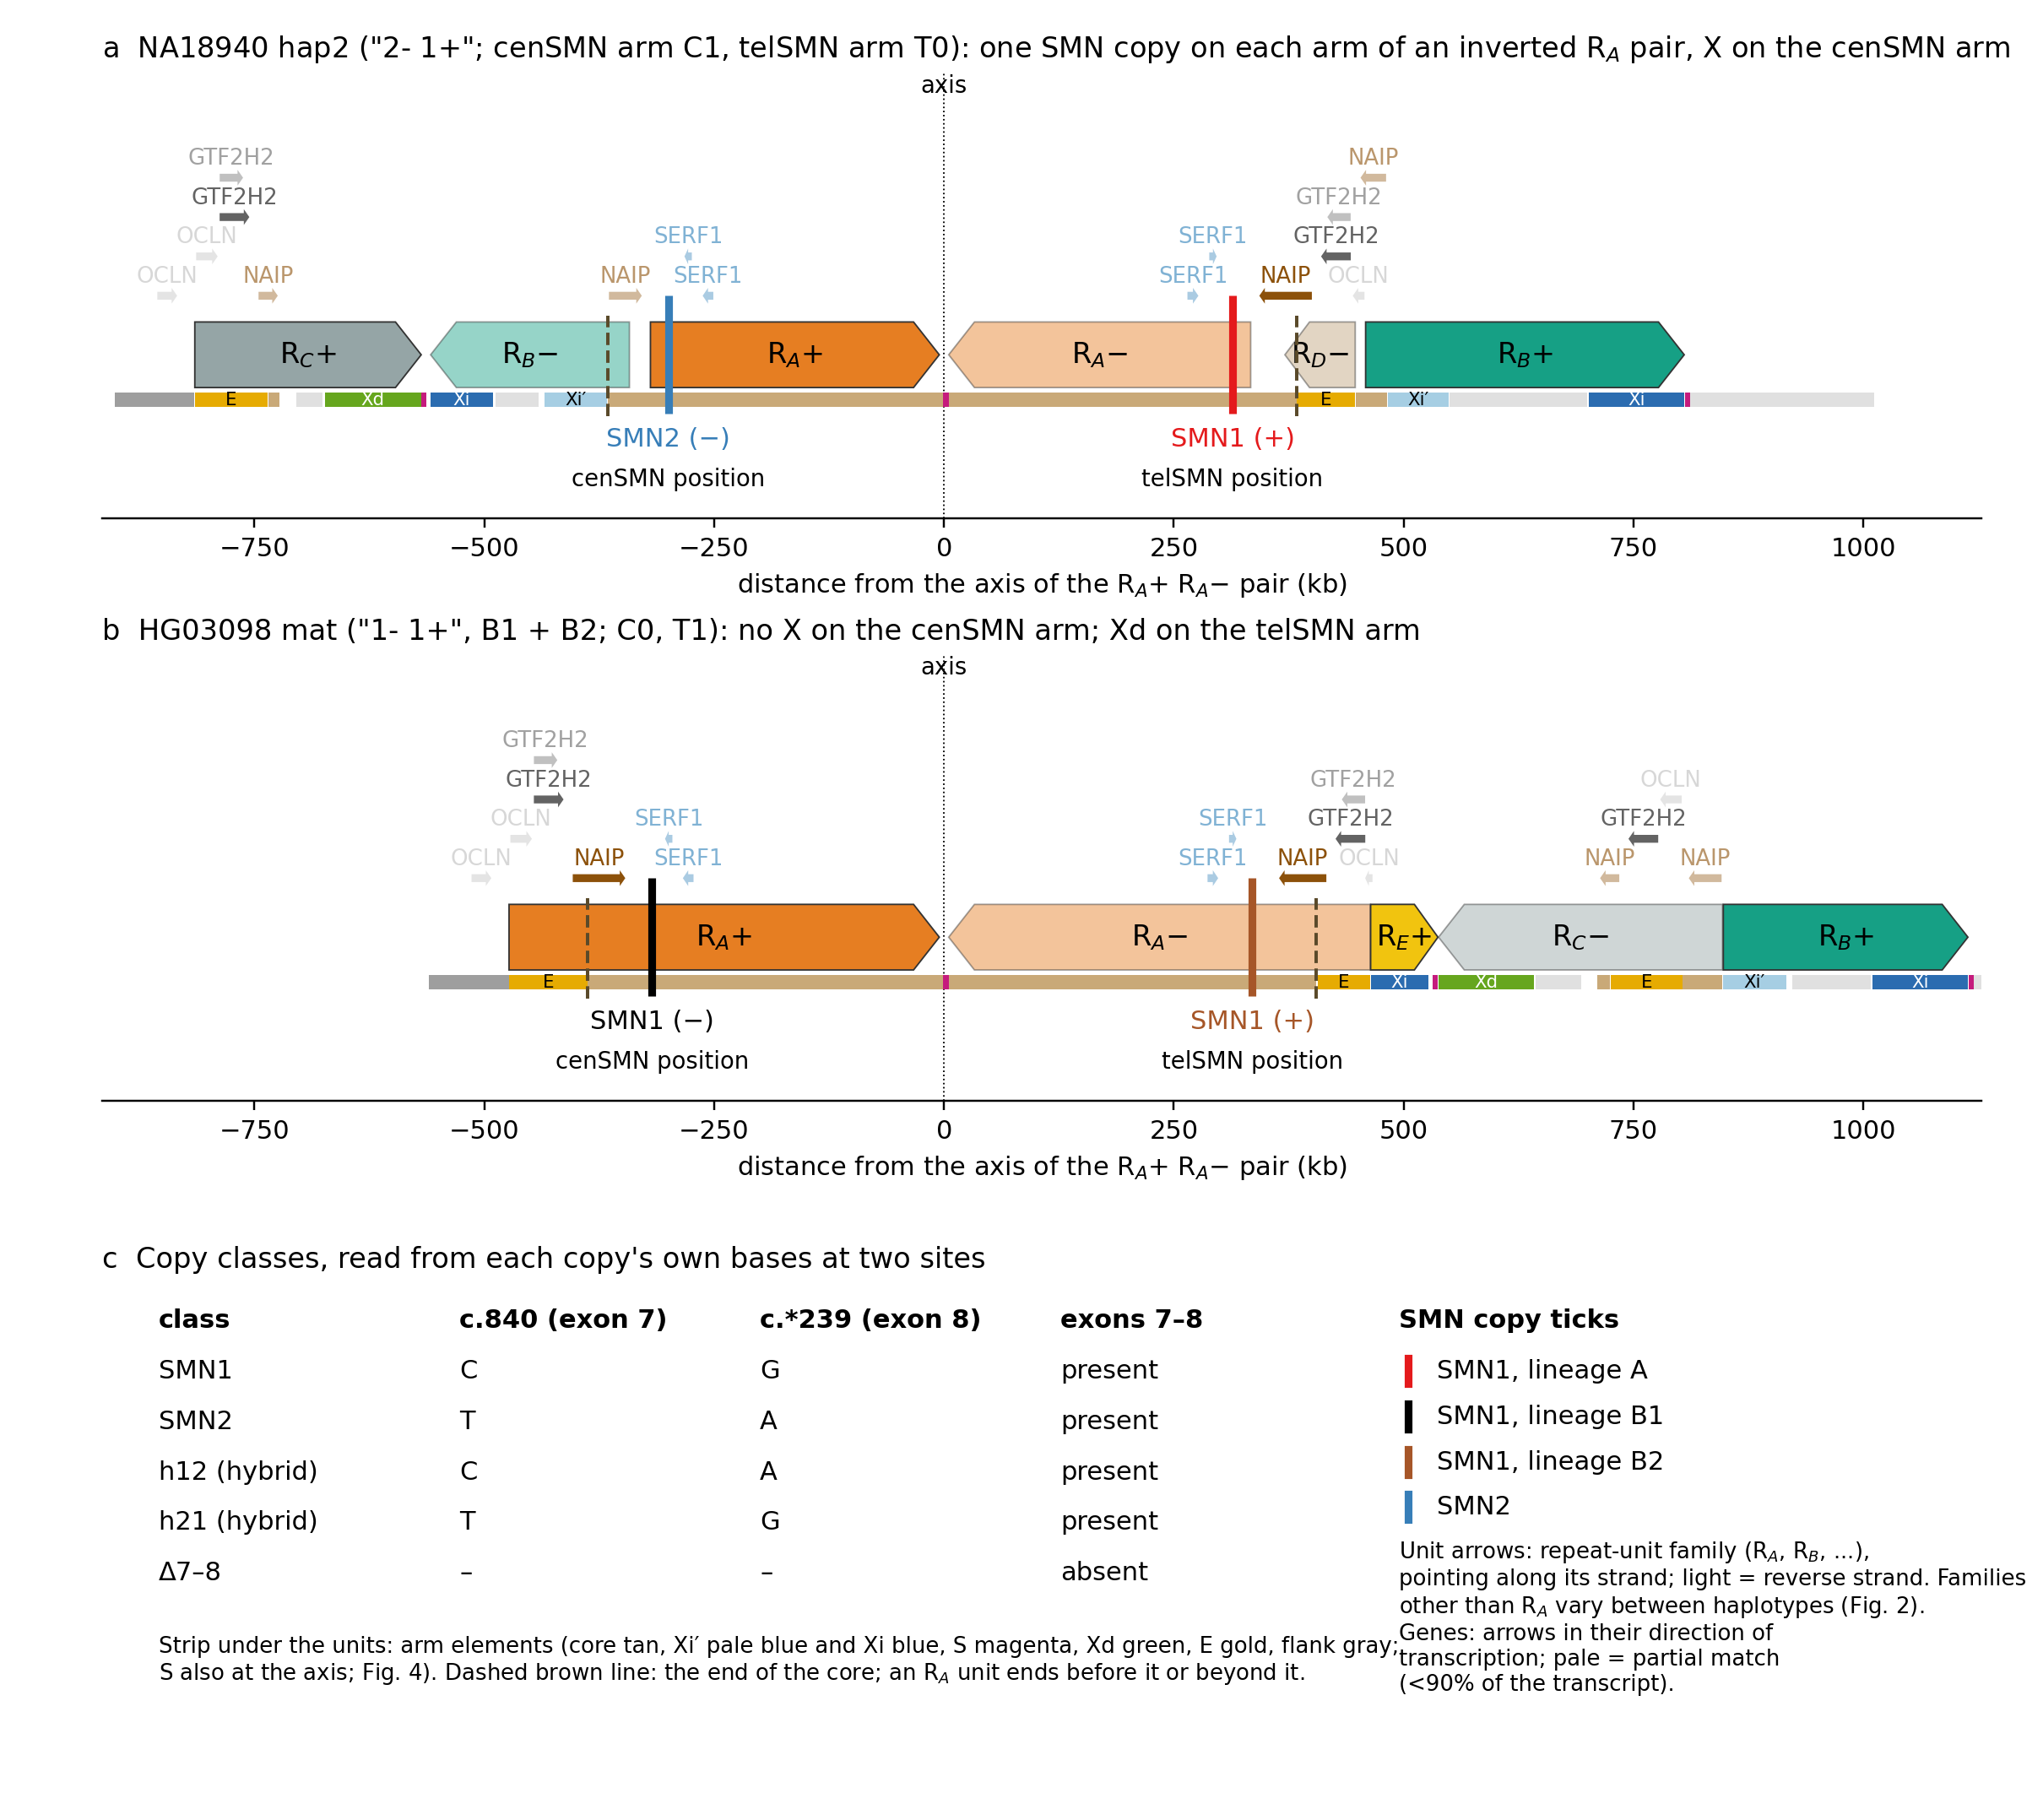
\includegraphics[width=\linewidth]{../figures/locus_diagram.png}
\caption{The SMN region as this study defines it (haplotype names as in Section~\ref{m:arr}). \textbf{a}, \dpAName{}, a ``2-~1+'' haplotype whose cenSMN arm
carries X (type C1) and whose telSMN arm is type T0 (arm types, defined in Section~\ref{m:arms}: C1 or C0, cenSMN arm with or without Xd, and so with or without X, the element made of Xi, S and Xd, which on all but \xcNoS{} C1 arms is whole; T0 or T1, telSMN arm without or with Xd, a direct copy of core sequence beyond the spacer S), drawn to scale around the axis of its head-to-head pair of
\RU{A} repeat units (\RU{A}+ then \RU{A}$-$): repeat units as bars labeled by family and strand (light, reverse strand; the
whole assembled window is drawn; every haplotype's units are in Fig.~\ref{fig:allhaps}), the genes found in the window
as arrows in their direction of transcription (pale where the match covers less than 90\% of the transcript), and the
two SMN copies as ticks colored by gene and SMN1 lineage (A, B1, B2; Section~\ref{m:lineages}), one on each arm, at the cenSMN (left) and telSMN (right)
positions. The strip under the units gives the arm elements of Section~\ref{m:arms}: the core (tan, from the axis to the end
of the core), Xi$'$ (pale blue) and Xi (blue), the inner and outer parts of an inverted copy of the core beyond the core, of which Xi, S and Xd make X, the spacer S (magenta, also at the axis), Xd (green), E (gold; the stretch, carrying \emph{GTF2H2}, that follows a copy of the core's end) and
the unique flank (gray). On the cenSMN arm of (a) the partial \emph{NAIP} at the end of the core and the one beyond X, next to
E, are the two parts of one gene split by X. \textbf{b}, \dpDName{}, a ``1-~1+'' haplotype with one copy of each of the SMN1 sub-lineages B1 and B2 (Section~\ref{m:lineages}),
 whose cenSMN arm lacks X (type C0; \emph{NAIP} whole) and whose telSMN arm carries Xd (type T1). Neither
haplotype carries a hybrid copy. Both are chosen by rule (Methods). \textbf{c}, the copy classes, read from each
copy's own bases at c.840 and c.*239 (definitions only; the tick colors are listed beside them). Gene labels: \emph{GTF2H2C}, GTF2H2 family member~C; \emph{OCLN}, occludin. Each repeat unit is drawn as an arrow pointing along its strand, so the \RU{A}+ and \RU{A}$-$ units point head to head at the axis and the inverted and direct copies beyond them read off by direction. Unit-family
colors are the same in Figs.~\ref{fig:locus} and \ref{fig:allhaps}. Repeat-unit families are written \RU{A}, \RU{B}, \dots{} (with a strand, as \RU{A}+ or \RU{B}$-$). The \RU{A} units of (a) and (b) differ in length (\auAcenUnit{} and \auAtelUnit~kb against \auDcenUnit{} and \auDtelUnit~kb; each unit begins about \dpAxisGap~kb from the axis, so the drawn units reach that much further) far more than their cores do (to the end of the core \auAcenCore{} and \auAtelCore~kb against \auDcenCore{} and \auDtelCore~kb): a unit ends where the two arms stop matching in mirror image, which in (b) is beyond the core's end and E, present on both arms, and in (a) before the core's end, because the cenSMN arm continues with X instead (Section~\ref{m:arms}).}
\label{fig:locus}
\end{figure}

\begin{figure}[p]\centering
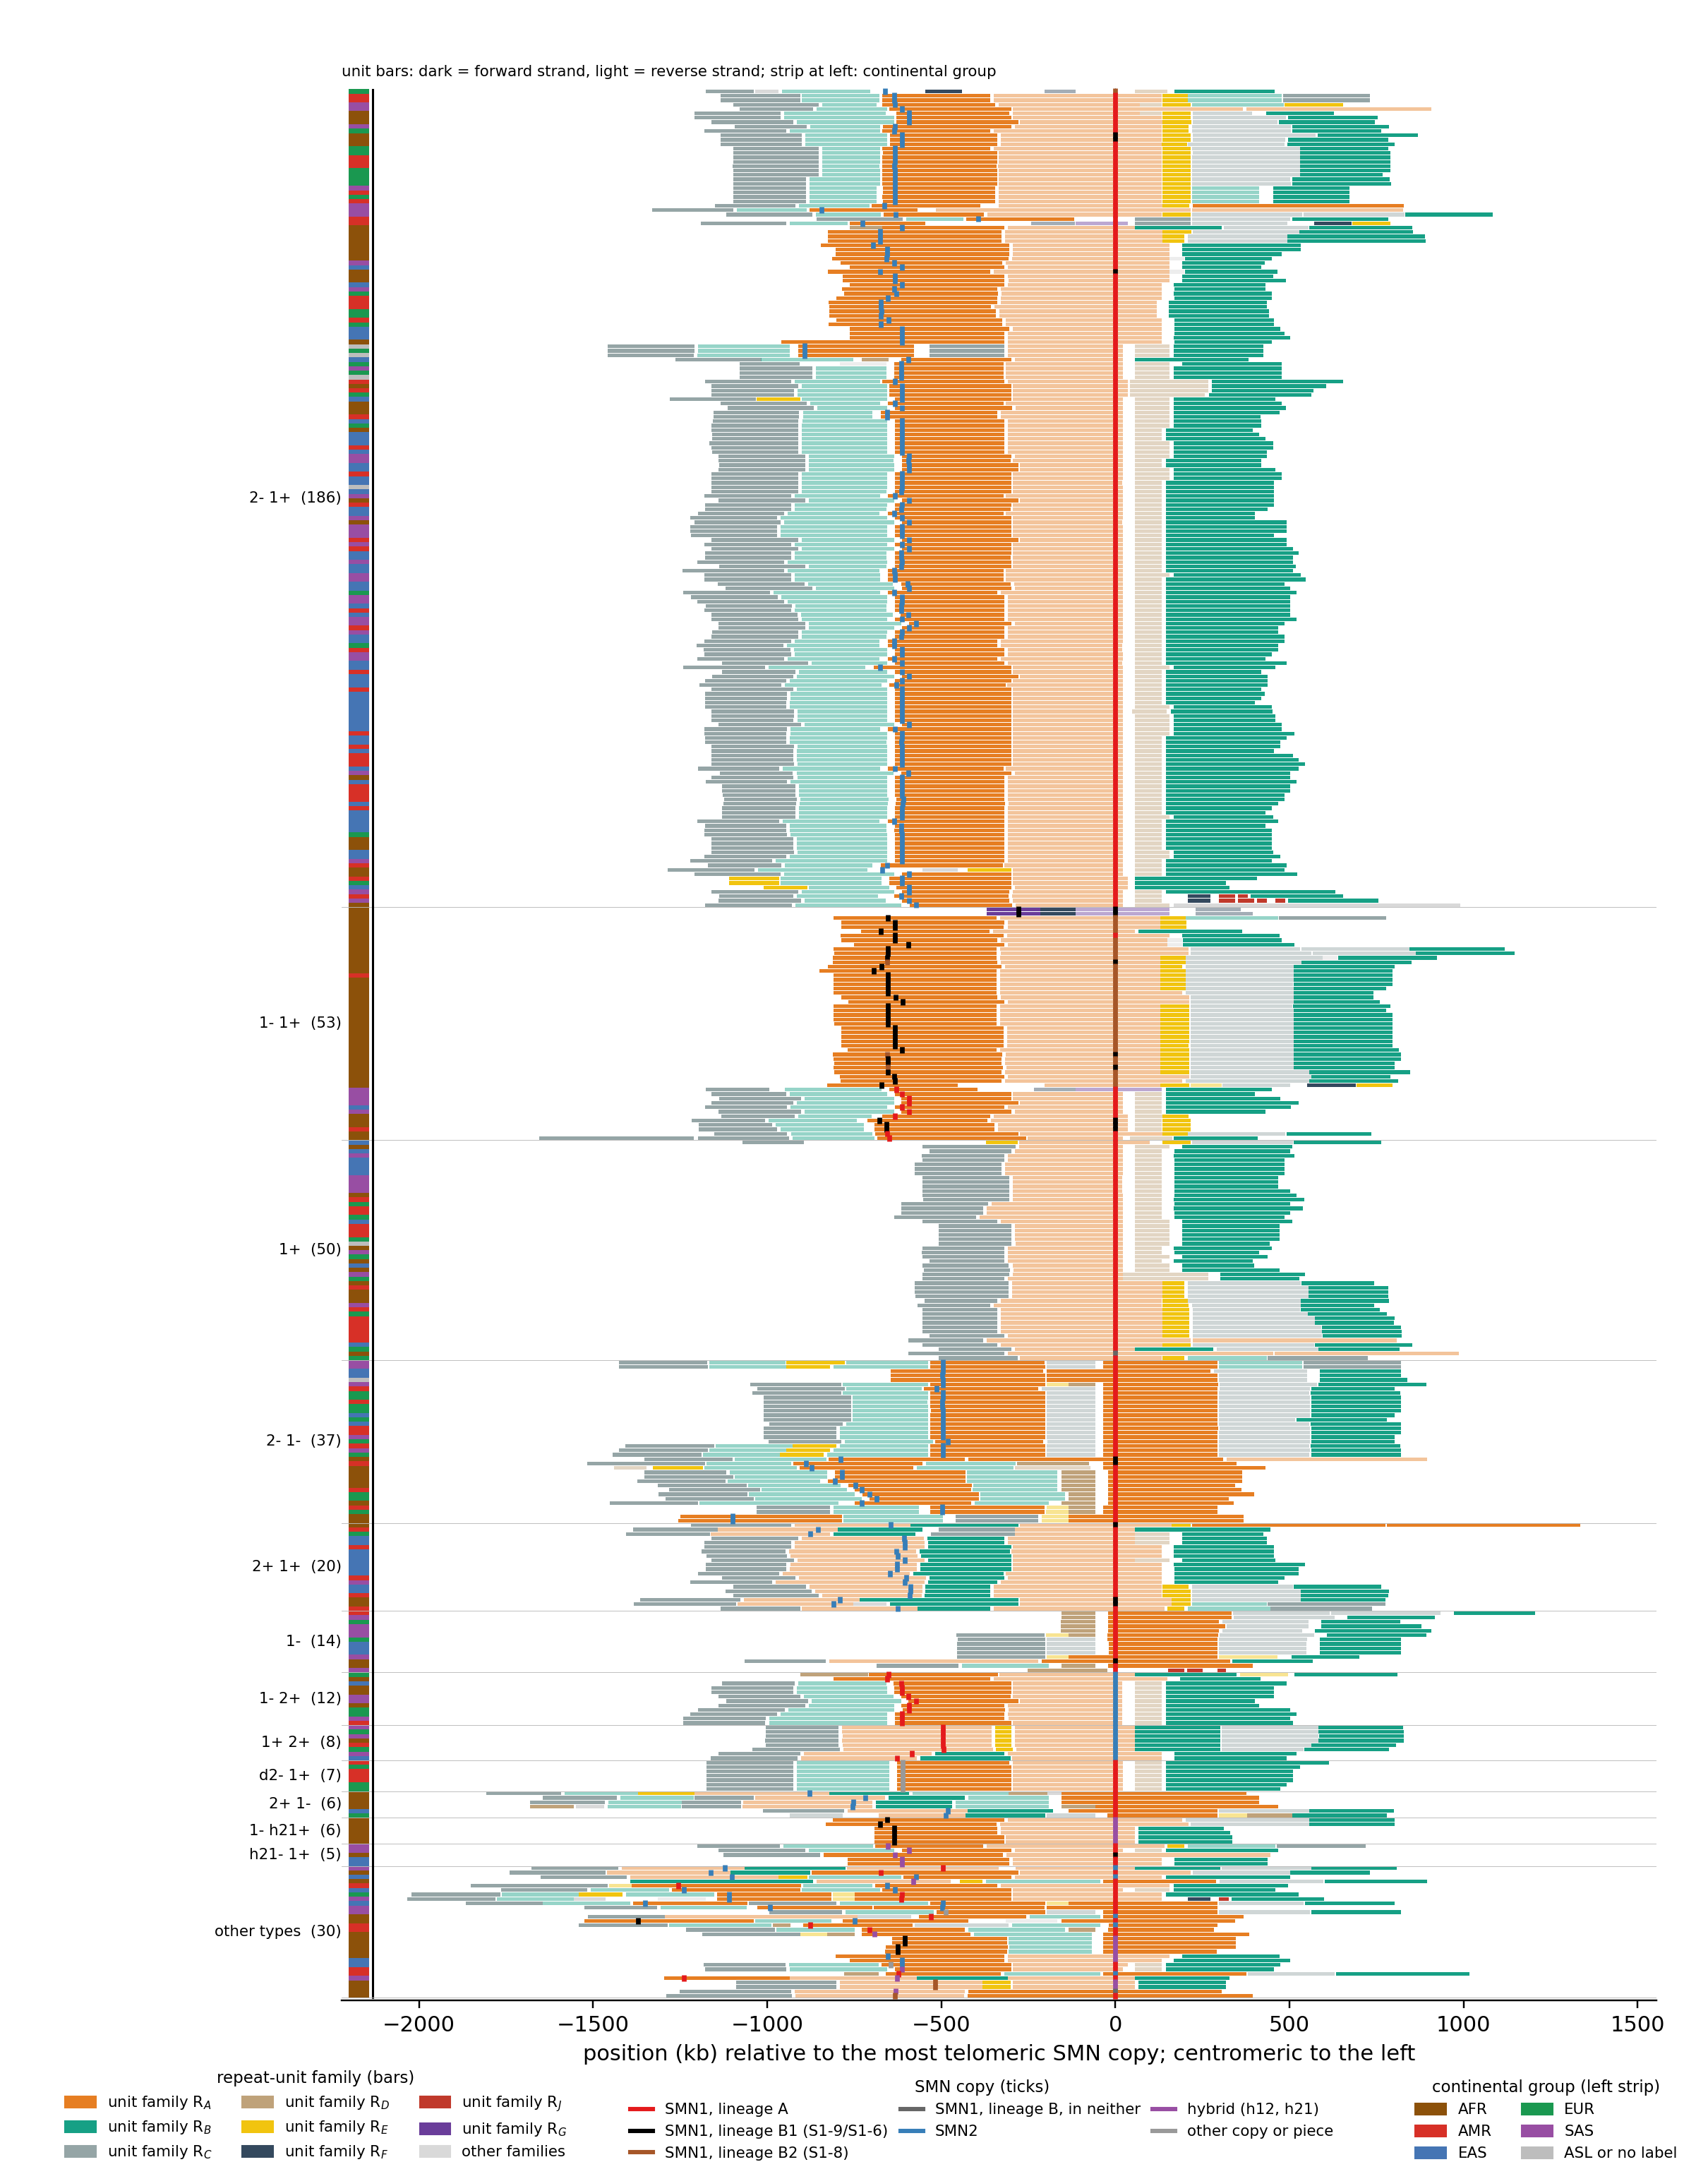
\includegraphics[width=\linewidth,height=0.78\textheight,keepaspectratio]{../figures/all_haplotypes.png}
\caption{Every resolved haplotype whose window PANGEA decomposed into repeat units, one row each (the \nHapsNoUnits{} resolved haplotypes without units, Section~\ref{m:arr}, are not drawn), aligned on its most
telomeric SMN copy (x = 0) and grouped by arrangement type (haplotype counts at left; types on fewer than five
haplotypes pooled; in the type codes a number or letter names the copy, 1 SMN1, 2 SMN2, h12 and h21 the hybrids, d2 a $\Delta$7--8 copy of SMN2 type, t a truncated copy and f a fragment (one haplotype each), and $+$/$-$ its strand, Supplementary Section~\ref{sec:compared}). Bars: large repeat units colored by family (each family defined by its bundle content in Supplementary
Table~\ref{tab:unitfam}), dark for the forward and light for the reverse strand. \RU{A} units end near the end of the core, before it or beyond the E that follows it depending on the arm type (Section~\ref{m:arms}); what the arms hold beyond the core is read from
their elements (Section~\ref{m:arms}). Ticks: SMN copies, colored by class, with SMN1 split into lineage A (red) and the B sub-lineages B1 (black) and B2
(brown; Section~\ref{m:lineages}). Left strip: continental group of the donor (1000 Genomes superpopulation; ``ASL or no label'' marks the one donor whose population code in the HPRC sample table is ASL, which is not one of the 1000 Genomes population codes, and the two donors with no population label). Within an arrangement group, rows are ordered by
UPGMA (unweighted pair-group average-linkage clustering; Sokal and Michener, 1958) on the structural distance between windows (PANGEA's bundle distance, defined in Methods and Supplementary Section~\ref{sec:compared}).}
\label{fig:allhaps}
\end{figure}

\subsection{SMN1 copies fall into two lineages; lineage B, almost only African, has two sub-lineages}\label{m:lineages}
The \nCopies{} whole counted copies, from every haplotype including \nCopiesUnres{} copies on \nCopiesUnresHaps{} haplotypes not resolved end to end (\nSMNone{} SMN1, \nSMNtwo{} SMN2, \nHtwentyone{} h21 and \nHtwelve{} h12; the
\nDelLeftOut{} $\Delta$7--8 copies and \nJoined{} copy joined from two pieces left out, Methods) were aligned over the \nGeneCols{} columns of the multiple alignment
that lie between the 2-kb flanks (the gene body; Supplementary Section~\ref{sec:compared}). A maximum-likelihood (ML) tree
with \iqBoot{} ultrafast bootstrap replicates (a clade's support is the percentage of the \iqBoot{} replicate trees that contain it), rooted on the orangutan copy with the chimpanzee, bonobo and gorilla copies
included (the ape copies do not fall in species order, so the root is uncertain; Section~\ref{m:hist}), divides the human copies into two halves (Fig.~\ref{fig:mltree}): one of \mlIcopies{} copies (support
\mlIsup) holding \mlIB{} SMN1 copies and \mlIh{} h21 copies, and one of \mlIIcopies{} copies (support \mlIIsup)
holding the other \mlIIA{} SMN1 copies, all \mlIISMNtwo{} SMN2 copies, \mlIIh{} h21 and \mlIIhtwelve{} h12 copies. We
call the SMN1 copies of the first half \emph{lineage B} and those of the second \emph{lineage A}. Within B's half two
clades are supported: \emph{B1}, \linBone{} SMN1 copies together with the \mlBhH{} h21 copies (support \mlBhSup), and
\emph{B2}, \linBtwo{} SMN1 copies (support \mlEightSup); \linBnone{} B copies fall in neither. B2 is nearer A in p-distance (the share of differing bases between two copies, over the columns where both carry a base; \gsABtwo{} differences per kb) than it is to B1 (\gsBoneBtwo; Supplementary Section~\ref{sec:grpdist}). The maximum-likelihood tree puts B1 and B2 in one half (\mlIcopies{} copies, support \mlIsup, with the \linBnone{} B copies of neither clade), but the node that joins B1 and B2 alone (\mlBBjoinCopies{} copies) has support \mlBBjoinSup.

The lineages coincide with Chen et al.'s SMN1 haplogroups, found from PacBio HiFi (high-fidelity long) reads with Paraphase~\cite{chen2023}, whose
``haplotype'' is one gene copy rather than one chromosome. B1 holds all \hgNineB{} copies of the S1-9 family (S1-9,
S1-9c, S1-9d) and \hgBoneSix{} of the \hgSixB{} S1-6 copies (S1-6 with its subgroup S1-6c), B2 all \hgEightB{} S1-8 copies, and the \hgBnoneSix{} B
copies in neither clade are S1-6; no copy of these three haplogroups is in lineage A (Supplementary
Table~\ref{tab:chenhg}). In each of the \hgPeople{} people the two studies share, our B count equals each person's
number of S1-6, S1-8 and S1-9 copies. B is found in all \ldAfrPopsB{} African-ancestry populations sampled, at
\ldShareMin--\ldShareMax\% of SMN1 copies in the \ldAfrPopsBig{} with ten or more, and outside them only in
\linBNonAfrPops{} SMN1 copies; \linBAfr{} of the \linB{} B copies come from African-ancestry donors.

Compared pair by pair over the gene body (Supplementary Section~\ref{sec:grpdist}), lineage A is \gdATwoMean{}
differences per kb from SMN2 and \gdABMean{} from B. Within B, B1 is the copy group furthest from SMN2
(\gsBoneTwo), B2's distance from SMN2 lies between those of A and B1 (\gsBtwoTwo), and B1 and B2 are \gsBoneBtwo{} apart. B2 is the least varied group
(\gsBtwoBtwo{} within it), then B1 (\gsBoneBone); A and SMN2 vary equally (\gsAA{} and \gdTwoTwoMean).

The lineages differ at \abCols{} gene-body columns of the multiple sequence alignment (MSA), where the commonest states of A and B differ; adjacent columns of one insertion or deletion count as one event, leaving
\abEvents{} events (\abSNV{} base changes and \abIndel{} insertions or deletions), mostly in intron~1 (\abIntronOne{} events) and
intron~6 (\abIntronSix{} events; Supplementary Fig.~\ref{fig:absites}); SMN2 carries lineage A's state at \abSmnTwoA{} of them and B's at \abSmnTwoB. At \abNearFixed{} events each lineage carries its own
state in at least 90\% of its copies, and at \abPerfect{} in every copy: \abPerfOneKind{} at chr5:\abPerfOnePos{} in
the 5$'$ untranslated part of exon~1 (\abPerfOneC, \abPerfOneBefore{} bases before the start codon) and \abPerfTwoKind{} at chr5:\abPerfTwoPos{} in intron~1. None
lies in the coding sequence. The marker \cpe{}, in intron~7, is on \linBoneMk{} of the \linBone{} B1 copies,
\linBtwoMk{} of the \linBtwo{} B2 copies and no A copy. Because the lineages were cut from a tree built on the same
alignment, how cleanly these sites separate them is partly built in and needs testing in other samples.

\begin{figure}[p]\centering
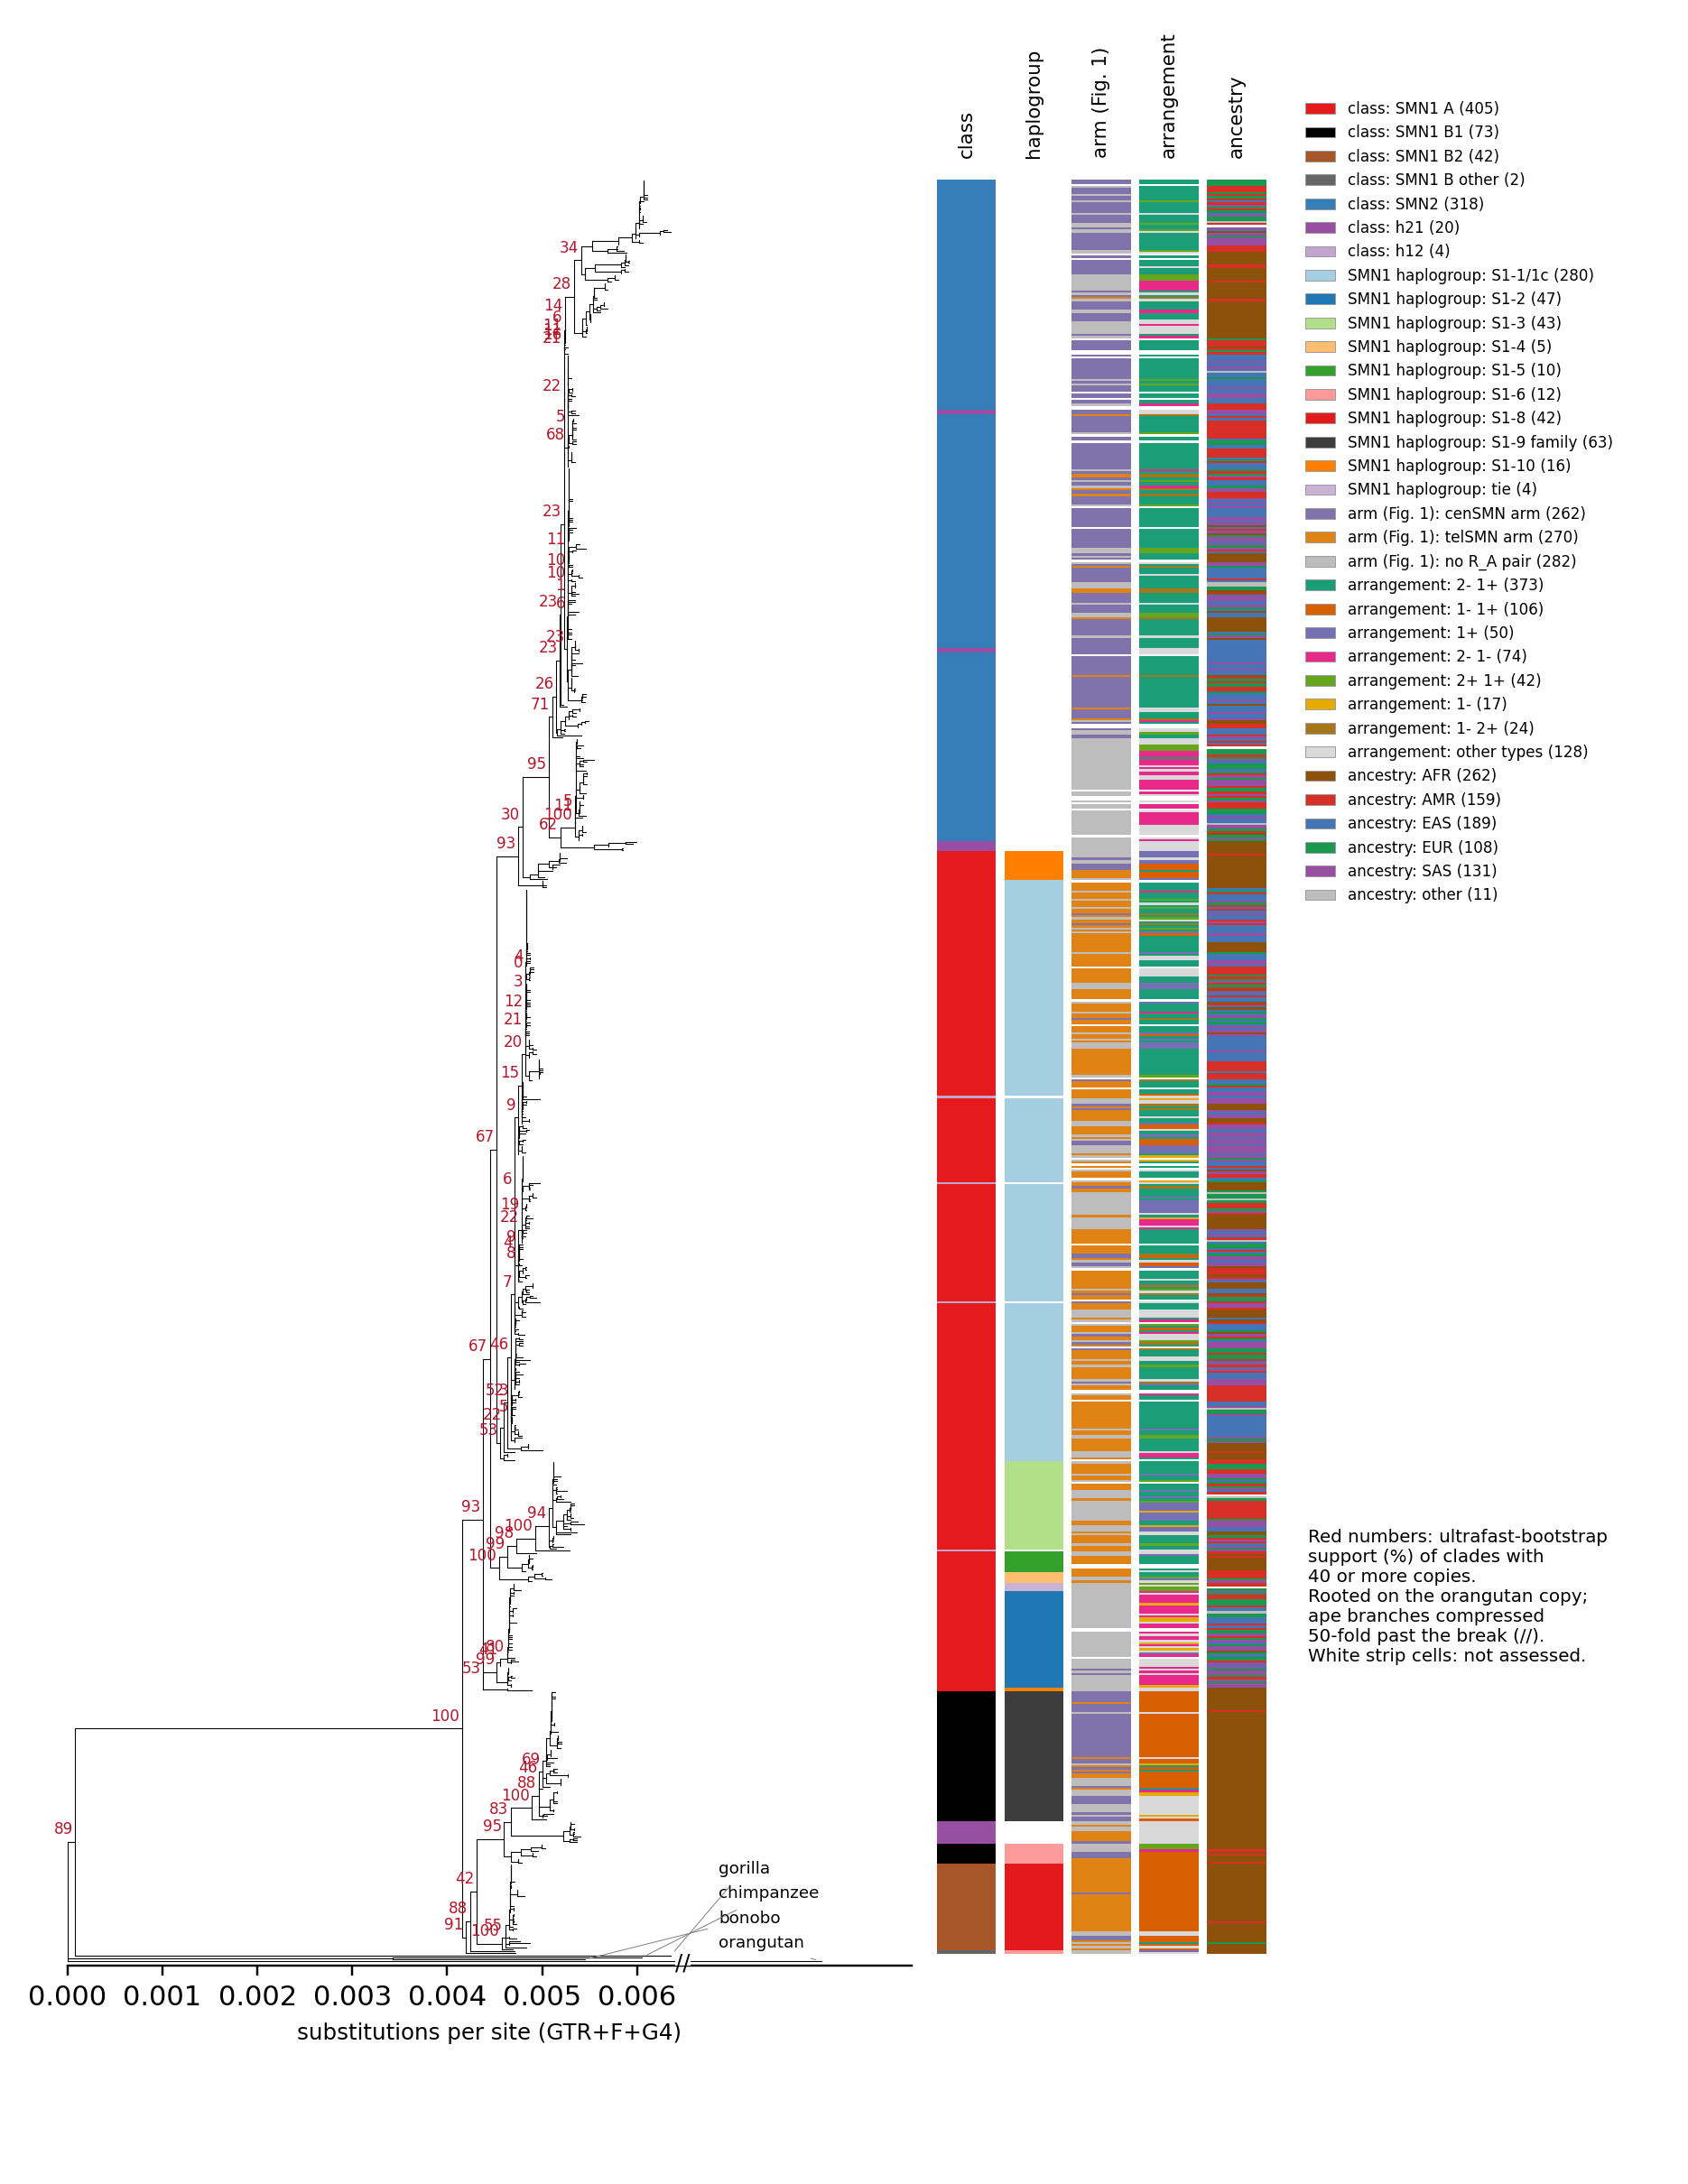
\includegraphics[width=\linewidth,height=0.80\textheight,keepaspectratio]{../figures/ml_tree.png}
\caption{Maximum-likelihood tree of the \nCopies{} SMN copies over the gene body (IQ-TREE, \iqModel: the general time-reversible substitution model with base frequencies from the data and four gamma-distributed rate categories), rooted on the
orangutan copy, with the chimpanzee, bonobo and gorilla copies; the ape branches are compressed past the break. The ape copies do not fall in species order (the gorilla copy is sister to the human copies, ultrafast bootstrap support \mlGorSup\% of \iqBoot{} replicates), so the root is uncertain.
Red numbers, ultrafast-bootstrap support (percentage of \iqBoot{} replicate trees) of clades of \setSupMin{} or more copies. Strips, one row per copy: class, with SMN1
split into lineage A (red) and sub-lineages B1 (black) and B2 (brown); Chen et al.'s SMN1 haplogroup; arm, as in Fig.~\ref{fig:locus}: the cenSMN or telSMN arm of the head-to-head \RU{A} pair that holds the copy, or `no \RU{A} pair' for a copy on a resolved haplotype without that pair (the cenSMN count is the \armCenInTree{} of the \armCenItems{} items on that arm, as in Fig.~\ref{fig:palindrome}, that are in the tree; the other \armCenNotTree{} are not: \armCenNTDel{} $\Delta$7--8 copies, \armCenNTTrunc{} truncated piece and \armCenNTComp{} SMN2 copy assembled from two pieces (\armCenNTCompHap), none of which is a whole copy (Methods; the trees use the whole copies); blank for the \nCopiesUnres{} copies on the \nCopiesUnresHaps{} haplotypes not resolved end to end);
arrangement type of the copy's haplotype, as in Fig.~\ref{fig:allhaps}, with types found on fewer than 10 resolved haplotypes pooled as `other types' (blank as for arm; Fig.~\ref{fig:allhaps} pools at fewer than five, so its `other types' is a smaller set); continental group of the donor (legend counts are copies, not haplotypes; the \spNone{} copies of GRCh38 and CHM13 have no group and are not counted).}
\label{fig:mltree}
\end{figure}

\subsection{The common African two-copy SMN1 allele is a head-to-head pair of B1 and B2}\label{m:cen}
The assemblies give each copy's place in its haplotype, which alignments of reads to a reference cannot tell. Lineage A is mostly telomeric (\linATel{} telomeric and \linACen{} centromeric copies; a copy's place here is its order among the window's SMN copies, Supplementary Section~\ref{sec:posstrand}, not the arm labels of Section~\ref{m:arms}, and the copies left over are single or middle copies or lie on haplotypes not resolved end to end), while B is found in both places (\linBCen{} centromeric,
\linBTel{} telomeric). The sub-lineages separate the two: B1 is centromeric in \linBoneCen{} copies, every one reversed (on a palindrome haplotype the centromeric copy always reads reversed; Supplementary Section~\ref{sec:posstrand}),
and telomeric in \linBoneTel; B2 is telomeric in \linBtwoTel, every one forward, and centromeric in \linBtwoCen{}
(two-sided Fisher exact $p=$\,\linSubPpos; Supplementary Section~\ref{sec:posstrand}). On the \linMixHaps{}
haplotypes that carry one B1 and one B2 copy (all \linMixHaps{} ``1-~1+'', \linMixAfr{} of them from African-ancestry donors), B1 is
centromeric and reversed on \linMixBoneCenRev{} and B2 telomeric and forward on \linMixBtwoTelFwd: Chen et al.'s common African two-copy allele (S1-8 with S1-9d; their Table~2)~\cite{chen2023}, whose two haplogroups fall in B2 and B1 (Section~\ref{m:lineages}), is, on the assemblies, the head-to-head inverted pair
with B1 at cenSMN and B2 at telSMN; on the other \linMixSwap{} (\linMixSwapNames) the two sit the other way round, B1 at telSMN and B2 at cenSMN. The test below uses the \mOneAFRN{} resolved AFR haplotypes with an SMN1 copy (the \dosAfrHaps{} resolved AFR haplotypes less the \dosAfrNoSmnOne{} with none). Of the
\ldTestBN{} of them that carry a B copy, \ldTestBMulti{} have two or more SMN1 copies,
against \ldTestNoBMulti{} of the \ldTestNoBN{} without one (Fisher $p=$\,\ldTestP); read the other way,
\ldTestBMulti{} of the \ldTestMultiN{} AFR haplotypes with two or more SMN1 copies carry B.

On the inverted \RU{A} pair (Fig.~\ref{fig:palindrome}a,c; Supplementary Table~\ref{tab:slots}), the left (cenSMN) arm of AFR
haplotypes holds SMN1 B on \slLAfrB{} of \slLAfr{} (B1 on \slLAfrBone{}, B2 on \slLAfrBtwo; the table pools B), SMN2 on \slLAfrTwo{} and A on \slLAfrA, while in the other groups it
holds SMN2 on \slLOthTwo{} of \slLOth{} arms (the table counts \slLOthItems{} items there: one arm also carries a truncated piece); the right (telSMN) arm of AFR haplotypes holds B2 on \slRAfrBtwo{} and A on \slRAfrA{} of \slRAfr{} (the table pools B there too: \slRAfrBtwo{} B2 with \slRAfrBone{} B1), and in the other groups A on \slROthA{} of \slROth. In this cohort's African-ancestry haplotypes
the commonest gene at the cenSMN position is thus SMN1 of sub-lineage B1, not SMN2; Lefebvre et al.'s naming of the two
loci by position~\cite{lefebvre1995} fits most haplotypes outside Africa.

B1 is a sequence lineage, not a place in the window:
\linBoneTel{} B1 copies are telomeric, of the \linMkSingleB{} haplotypes whose only SMN1 copy is B, \linMkSingleBone{} carry B1 (\linMkSingleBtwo{} B2, \linMkSingleBnone{} a B copy in neither clade), and B1 also
forms SMN1 + h21 pairs, ``1-~h21+'' (\ldHtwoOnePlusN{} haplotypes) and ``1-~h21-'' (\ldHtwoOneMinusN), where every SMN1 copy is B1 (\ldHtwoOneBOne{} of \ldHtwoOneN); the \ldOnePHtwoOneN{} ``1+~h21+'' haplotypes carry B2 instead (Supplementary
Section~\ref{sec:lindetail}).

By arm, the cenSMN or telSMN arm of the head-to-head \RU{A} pair as in Fig.~\ref{fig:locus}, or no such pair (the `arm' strip of Fig.~\ref{fig:mltree}), B copies on the cenSMN arm are further from SMN2 than those on the telSMN arm (\dcBArmCen{} against \dcBArmTel{} differences per kb; Kruskal--Wallis test over the three arm groups, $p=$\,\dcPBArm), which reflects B1 against B2; B copies on haplotypes without the pair are \dcBArmNo. A copies on the two arms are equally far (\dcAArmCen{} and \dcAArmTel; \dcAArmCenN{} and \dcAArmTelN{} copies; the GRCh38 and CHM13 copies are left out of these tests), and A copies on haplotypes without the pair are slightly further (\dcAArmNo; three arm groups, $p=$\,\dcPAArm). A copies also differ by arrangement type ($p=$\,\dcPAArr) and, slightly, by whether a full \emph{NAIP} lies 3$'$ of the copy ($p=$\,\dcPANaip; medians \dcANaipSpread{} per kb apart), but these shifts are small: the arm moves the medians by at most \dcArmSpread{} per kb, and across arrangement types they run from \dcAArrMin{} to \dcAArrMax. Within AFR the arm difference of A is not seen ($p=$\,\dcPAfrAArm), while arrangement type still shifts the AFR A copies' medians, by up to \dcAfrArrSpread{} per kb ($p=$\,\dcPAfrAArr), a shift that comes from the \dcAfrArrOneOneN{} A copies on AFR ``1-~1+'' haplotypes (median \dcAfrArrOneOneMed{} against \dcAfrArrOthMin--\dcAfrArrOthMax{} for the other types) (Supplementary Section~\ref{sec:distctx}).

\begin{figure}[p]\centering
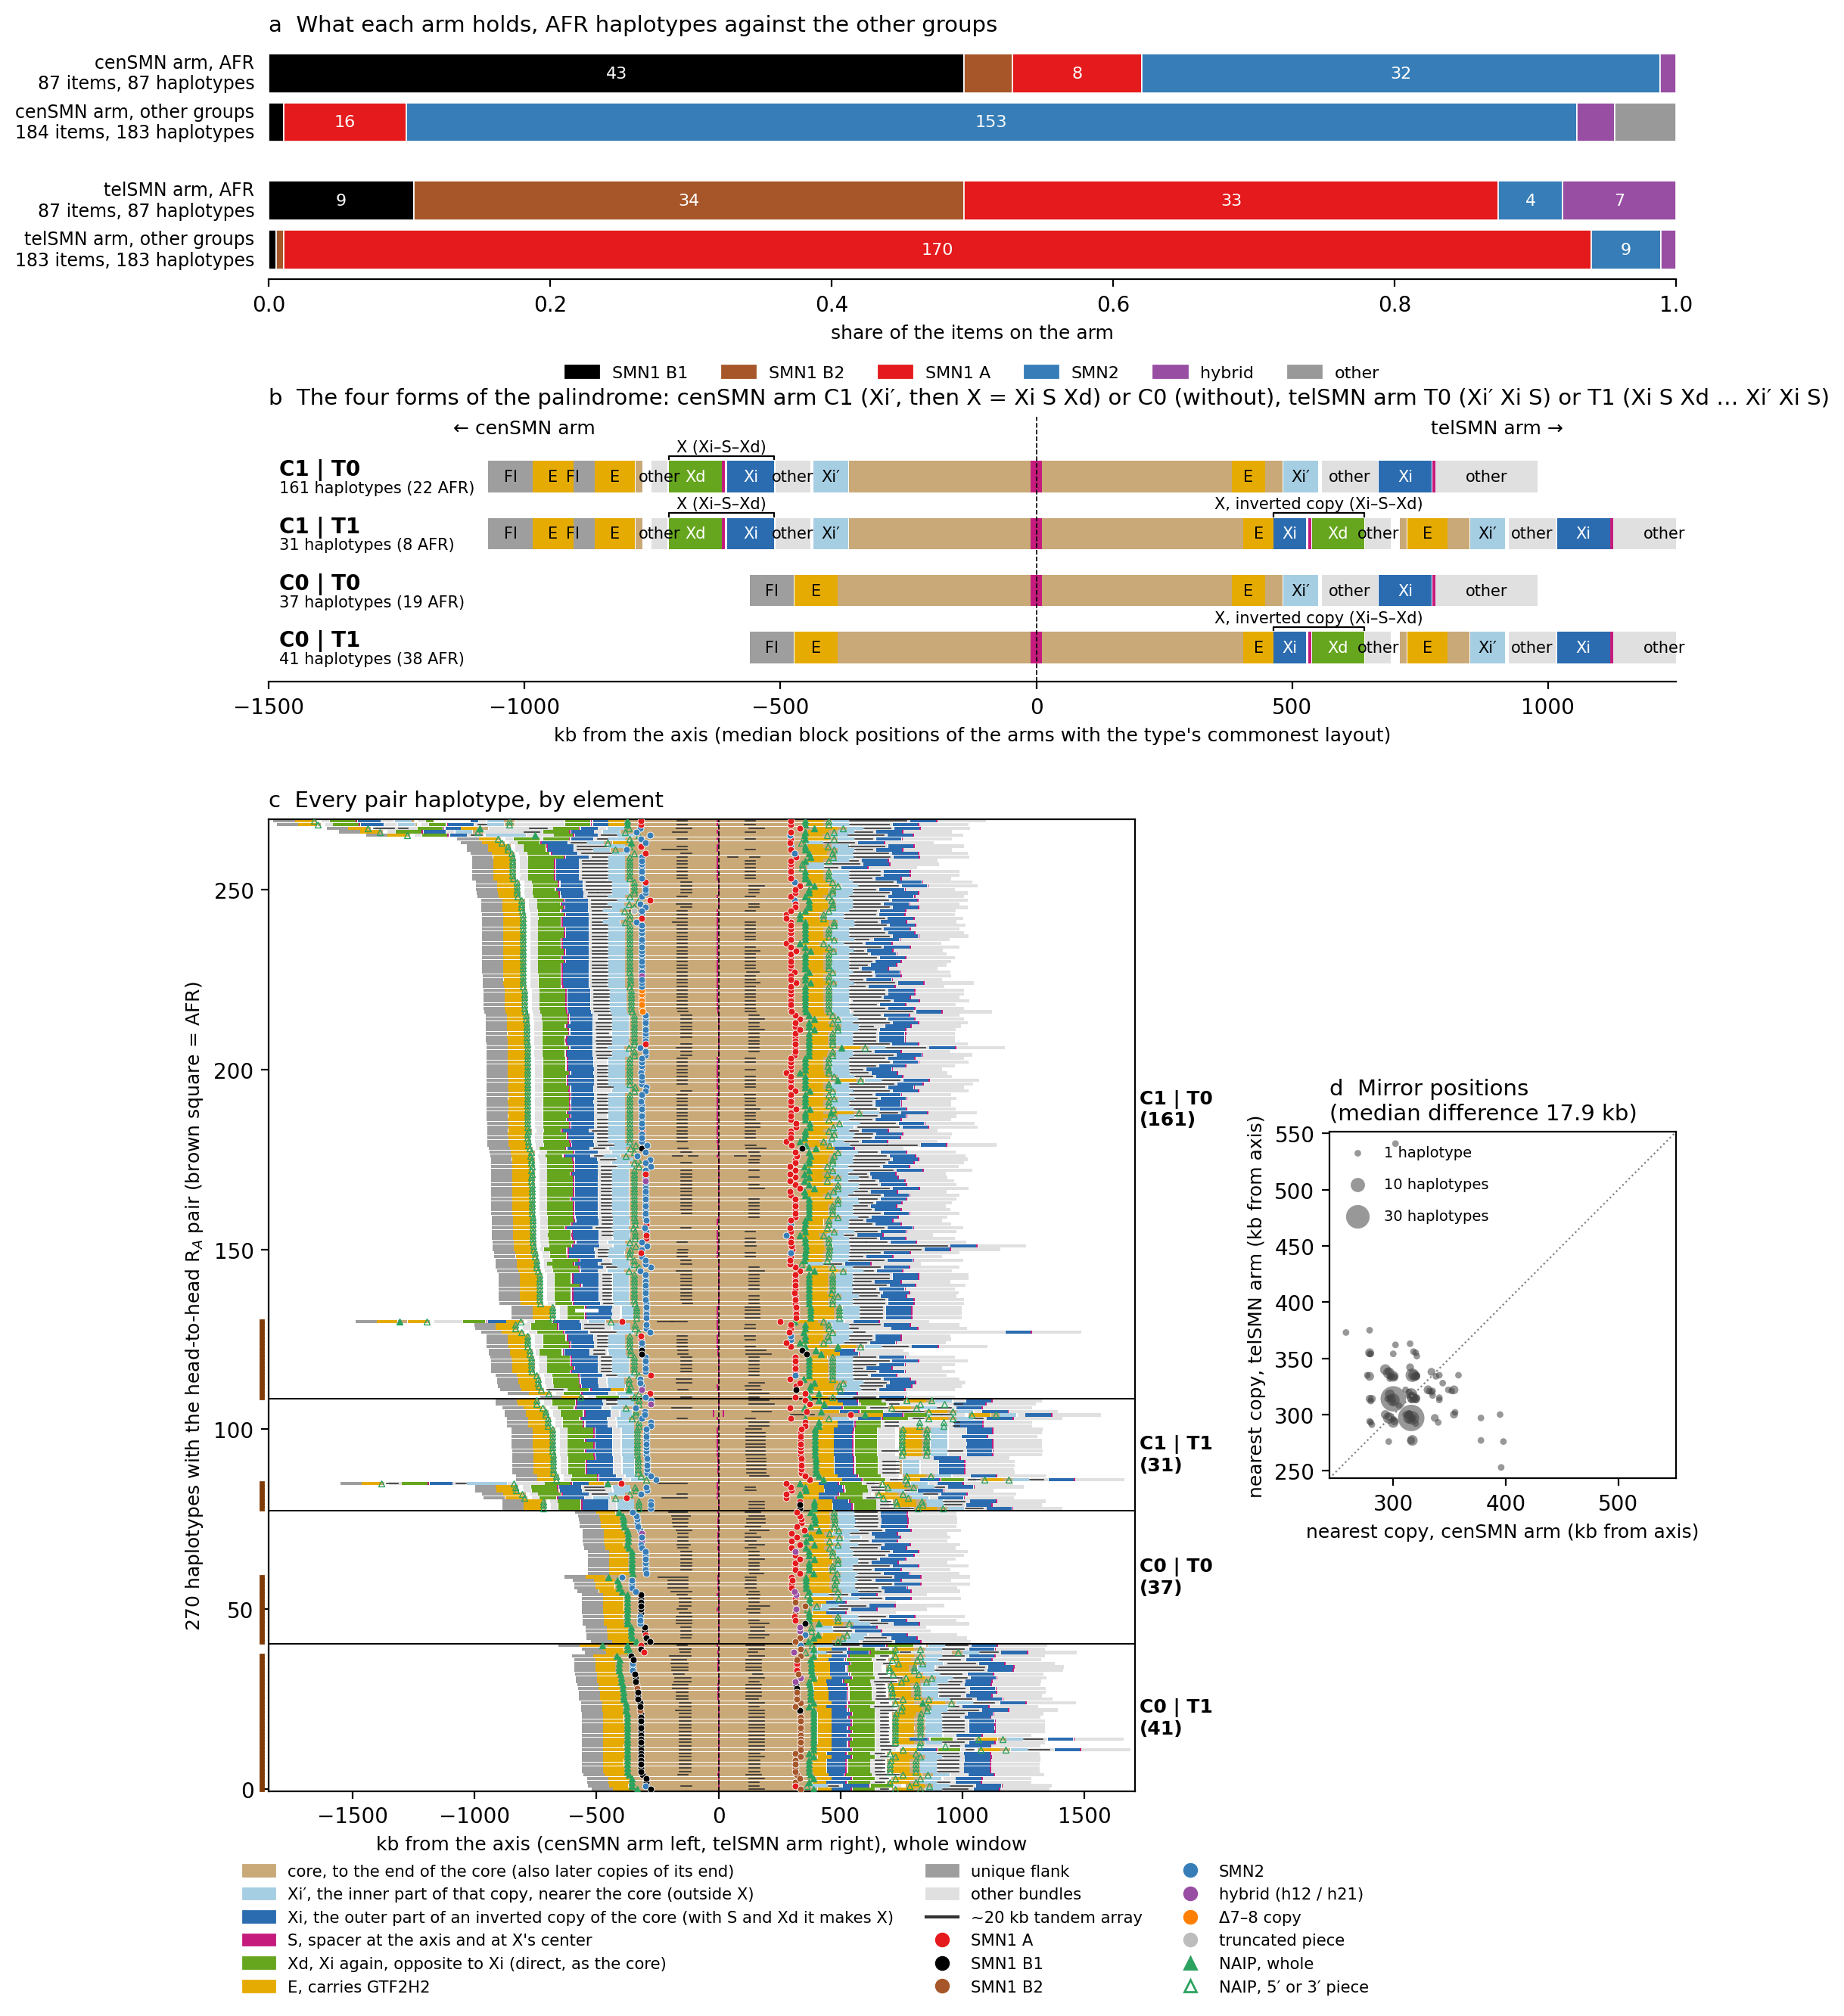
\includegraphics[width=\linewidth,height=0.88\textheight,keepaspectratio]{../figures/palindrome.png}
\caption{The \RU{A} palindrome read as named elements. \textbf{a}, what each arm holds: the items on the left
(cenSMN, \RU{A}+) and right (telSMN, \RU{A}$-$) arms of the AFR haplotypes and of those of the other groups, by gene and, for
SMN1, lineage (numbers in the bars are items; each arm holds one copy, and one arm also a truncated piece). On the
cenSMN arm of AFR haplotypes B1 is the commonest gene (\slLAfrBone{} of \slLAfr), ahead of SMN2 (\slLAfrTwo{} of \slLAfr); in the
other groups SMN2 holds it (\slLOthTwo{} of \slLOth). \textbf{b}, the four forms of the palindrome, cenSMN arm C1
(with Xd, and so X, the inverted repeat of Xi, S and Xd, whole on all but \xcNoS{} arms; Xi$'$ on nearly all) or C0 (none of them), telSMN arm T0 (Xi and S, with Xi$'$ on nearly all) or T1 (X, then Xi$'$, Xi and S further out), each drawn from the median block
positions (labels as in panel c; Fl, unique flank) of the arms with that type's commonest layout, with the number of haplotypes (AFR in brackets); brackets mark X (Xi--S--Xd) on C1 cenSMN arms and, on T1 telSMN arms, its inverted copy, which reads the same outward from the axis and so runs the opposite way along the window. \textbf{c},
all \palPair{} haplotypes with the palindrome (an adjacent \RU{A}+ \RU{A}$-$ pair with an SMN copy on each arm; Section~\ref{m:arr}), each a row aligned on its own axis (dashed) and colored by
element over its whole window, grouped by form; brown squares, AFR. Thin black lines, the $\sim$20-kb tandem arrays;
dots, the \palCopies{} items (red, SMN1 lineage A, \palSmnA; black, B1, and brown, B2, together \palSmnB{} B copies;
blue, SMN2, \fdSmnTwo; purple, hybrids, \fdHyb; orange, $\Delta$7--8 copies, \fdDel; gray, the truncated piece, \fdTrunc); triangles, \emph{NAIP} (filled, whole; open, a 5$^\prime$ or 3$^\prime$ part). Every copy stays
\palDmin--\palDmax~kb from the axis. \textbf{d}, for each haplotype the nearest copy on the left arm against the
nearest on the right; point size, number of haplotypes; points on the diagonal are exact mirrors (median difference
\palMirror~kb). Element ends, and so the axis, are known only to the resolution of PANGEA's bundles.}
\label{fig:palindrome}
\end{figure}

\subsection{The cenSMN arms differ by whether they carry X, which goes with a split NAIP; its absence goes with lineage B1}\label{m:arms}
Read bundle by bundle, with the bundles PANGEA identifies, the arms of the \RU{A} pair (here each side of the axis out to the end of the window, not the \RU{A} unit of Section~\ref{m:arr}) are a fixed series of named elements (Fig.~\ref{fig:locus}a; Fig.~\ref{fig:palindrome}b,c; Supplementary Section~\ref{sec:palindrome}). Walking outward from the axis, every arm begins with the core, which holds the arm's one counted SMN copy, whole or $\Delta$7--8 (\armOneCopy{} of \armN{} arms; Methods), and ends a median \elAEnd~kb out at a short run of bundles, the end of the core. Beyond it lie an inverted copy of the core, split by a $\sim$20-kb tandem array into an inner part, Xi$'$, nearer the core, and an outer part, Xi; S, a spacer of median \sLen~kb, which also sits at the main axis; Xd, a direct copy of Xi; E, a stretch carrying a whole \emph{GTF2H2} (\elGtfE{} of the \elGtfAll{} \emph{GTF2H2} matches lie in E); and the window's unique flank. Xi, S and Xd form an inverted repeat centered on S, which we call X, after its shape in a self dot plot: Xi and Xd draw a line across the diagonal that crosses it at S (Supplementary Fig.~\ref{fig:xcross}). Xi$'$ is not part of X: it has no partner across S, its partner being the core itself across the main axis, and with Xi it makes one inverted copy of the whole core, split by the array. On the cenSMN arm X runs from a median \xOutStart{} to \elCXdHi~kb from the axis and takes one of two lengths, \xFormShortKb{} or \xFormLongKb~kb (\xFormShortN{} and \xFormLongN{} of the \xSpanN{} arms with the commonest layout, none in between; \xFormBigN{} arms are longer, and the other \xSpanRest{} C1 arms carry an extra element and are not measured).

Each arm is one of two types, decided by Xd (C1 and T1 carry it, C0 and T0 do not). On the cenSMN arm \elCOne{} arms carry Xi and Xd, (type C1; \xpCOneBoth{} of them carry Xi$'$ as well); on all but \xcNoS{} of them (\xcNoSNames) S lies between the two, so that X is whole, and \elCZero{} carry none of them (type C0). On the telSMN arm Xi and S are always present: \elTZero{} arms lack Xd (type T0) and \elTOne{} carry it (type T1), there as an inverted copy of the cenSMN X. A haplotype's form pairs its two arm types, cenSMN arm first: C1|T0, C1|T1, C0|T0 or C0|T1 (Fig.~\ref{fig:palindrome}b). Where the \RU{A} unit of Section~\ref{m:arr} ends is set by what follows the core on each arm, so a long or short \RU{A} unit reports the arm type beside it, not a longer or shorter core (Supplementary Section~\ref{sec:palindrome}).

Xi$'$ and X split \emph{NAIP}. The gene spans the end of the core: on every C0 arm (\elNaipWholeCZero{} of \elCZero) a whole \emph{NAIP} crosses it and ends a median \elNaipPast~kb beyond. On \elNaipSplit{} of the \elCOne{} C1 arms the gene is cut there: a 3$^\prime$ part ends at the end of the core, and a 5$^\prime$ part lies beyond X, at the next copy of the core's end, next to E. Both cuts fall at exon junctions of the \emph{NAIP} transcript \nxTx{}, and the 5$^\prime$ part ends at codon \nxFiveCodon{} of \nxCodons, so it holds the first two of the protein's three BIR (baculovirus IAP repeat) domains and part of the third (Supplementary Section~\ref{sec:palindrome}). Per window, \elNaipTwoWholeCZero{} of the \elCZero{} haplotypes with a C0 arm have two whole \emph{NAIP} genes; \elNaipOneWholeCOne{} of the \elCOne{} with a C1 arm have one.

S is one element by sequence too, and comes in two variants: the S of X on the cenSMN arm matches the same haplotype's axis S (\sCenSa{} of \sCenAll; median \sSaMed{} differences per kb), while the S on the telSMN arm differs from it by a median \sStMed{} per kb (\sTelSt{} of \sTelAll{} compared; Supplementary Section~\ref{sec:palindrome}).

The SMN copy's distance from the axis rises with the number of units in a tandem array inside the core, of $\sim$\elInnerUnit-kb units (Spearman \elRhotel{} on the telSMN arm, \elRhocen{} on the cenSMN arm), and copies lie further out on T1 arms (median \elCopyDTOne{} against \elCopyDTZero~kb) and on C0 arms (\elCopyDCZero{} against \elCopyDCOne~kb). Campbell et al.\ saw differences of up to several hundred kilobases here by pulsed-field gels and proposed a tandem ``midisatellite'' array as their cause~\cite{campbell1997}; on the assemblies the arms differ by X and by the copy numbers of $\sim$20-kb tandem arrays at three places: inside the core, between Xi$'$ and Xi on C1 cenSMN arms, and between Xi$'$ and Xi on the telSMN arm (Supplementary Section~\ref{sec:palindrome}).

The arm types go with lineage and ancestry. C0 arms are common in AFR haplotypes (\elCZeroAfr{} of \elAfrHaps) and
rare elsewhere (\elCZeroNonAfr{} of \elNonAfrHaps). A B1 copy at cenSMN sits on a C0 arm on \elBoneCZero{} of
\elBoneCen{} arms; within AFR, \elAfrBoneCZero{} of \elAfrBoneCen{} B1 arms against \elAfrOthCZero{} of \elAfrOthCen{}
other cenSMN arms (Fisher $p=$\,\elAfrBoneP). All \elBB{} haplotypes with one B1 and one B2 copy have a C0 cenSMN arm,
and \elBBTOne{} of them a T1 telSMN arm; within AFR the telSMN arm of a B2 copy is T1 on \elAfrBtwoTOne{} of
\elAfrBtwoTel, against \elAfrOthTOne{} of \elAfrOthTel{} other telSMN arms ($p=$\,\elAfrBtwoP). The two types go
together (C0 with T1 on \elFzeroone{} haplotypes; Fisher $p=$\,\elFormP) within AFR ($p=$\,\elFormAfrP) but not
outside it ($p=$\,\elFormNonAfrP). Within AFR the link rests on the B1+B2 chromosome: left out, the two types no longer go together
(among the other \elFormAfrNoBBn{} AFR haplotypes, no association: the telSMN arm is T1 on \elFormAfrNoBBzPct\% of those with a C0 arm, \elFormAfrNoBBzt{} of \elFormAfrNoBBzN, against \elFormAfrNoBBoPct\% of those with a C1 arm, \elFormAfrNoBBot{} of \elFormAfrNoBBoN). Of the \elFzeroone{} C0|T1 haplotypes, \elFzerooneBB{} are B1+B2 and \elFzerooneNotBB{} are not. No EAS haplotype has a T1 arm.
The \elCZeroNotBB{} C0 arms on other haplotypes (\elCZeroNotBBAfr{} AFR) show that lacking X is not confined to it.

\subsection{Large-scale structure and SMN1 sequence go together in part, in bands of arrangement and haplogroup}\label{m:struct}
Haplotypes whose large-scale structure is similar (PANGEA's bundle distance over the whole window) carry similar SMN
copies: the rank correlation between the structural and sequence distances is \mantelAll{} over all copies (all \tsAllN{} windows, GRCh38 and CHM13 included), \mOneR{}
over SMN1 copies (the \mlbHaps{} haplotypes of Section~\ref{m:arr}) and \mTwoR{} over SMN2 copies, each $p\le$\,\mantelP{} (Mantel test, which compares the two distance matrices against \nPerm{} shuffles of the haplotypes in one of them, so $p$ is at the smallest value they can give; also with haplotypes shuffled only
within AFR and within non-AFR, or within each of five continental groups; Supplementary Section~\ref{sec:structseq}), though the two trees built from these distances
agree only loosely (cophenetic correlation \cophenetic, the correlation between haplotype-to-haplotype distances read off the structure tree and off the maximum-likelihood tree of Fig.~\ref{fig:mltree}; Supplementary Section~\ref{sec:cophen}). On the finer bundle
decomposition the link is a little stronger (\tsOneF{} over SMN1;
Supplementary Section~\ref{sec:fine}).

The agreement comes in bands: sets of haplotypes that fall together in one cluster of the structure tree and one
supported clade of the SMN1 maximum-likelihood tree (Methods; Supplementary Fig.~\ref{fig:tangclus}). Three form. One
holds \cbABn{} of the \linMixHaps{} ``1-~1+'' haplotypes that carry B1 and B2 (\cbABexp{} expected, $p=\cbABp$), each
with two divergent SMN1 copies, one per arm (Fig.~\ref{fig:palindrome}a,c): B1 and B2 differ by \gsBoneBtwo{}
differences per kb, nearly as much as lineage A differs from SMN2 (\gsATwo). A second holds \cbTwon{} haplotypes
whose one SMN1 copy lies in the supported ML clade that holds most S1-2 copies ($p=\cbTwop$), none from an African-ancestry donor and none with the head-to-head \RU{A} pair. The third is a loose bulk of
\cbBulkn{} haplotypes ($p=\cbBulkp$), mostly ``2-~1+'', whose SMN1 copy lies in no supported clade. The bands hold at each of
\mlbSettings{} settings of the clade thresholds (Supplementary Section~\ref{sec:bands}).

At the bundle decomposition used here, what splits the two largest of the \scN{} structure clusters (\scFirst{} and \scSecond{} haplotypes; the next holds \scThird) is the cenSMN arm type (Section~\ref{m:arms}); at a finer decomposition they split by the telSMN arm type instead (Supplementary Section~\ref{sec:fine}). Among the haplotypes with
the head-to-head \RU{A} pair, all \afBulkPair{} in the bulk band's cluster are C1 (carry Xi and Xd), and \afMixCZero{} of the
\afMixPair{} in the B1\,+\,B2 band's cluster lack it (C0; Fisher $p=$\,\afPC); every B1\,+\,B2 band haplotype is C0.
Within one arrangement type, pairs still separate largely by SMN1 haplogroup, in structure as well as in sequence
(Supplementary Section~\ref{sec:hgscatter}).


\subsection{The structure differs between continental groups, most between AFR and the rest}\label{m:anc}
Over \anHaps{} resolved haplotypes of \anPeople{} people in the five 1000 Genomes continental groups (the resolved haplotypes less the \anLeftOut{} of the three donors outside the five groups: the one coded ASL, not a 1000 Genomes population, and the two with no population label), arrangement
types differ between groups ($\chi^2=\anChi$, Cram\'er's $V=\anV$, a 0--1 measure of how strongly type and group are associated, \anPerm{} permutations of people, $p\le\anPArr$, the floor): ``2-~1+'' is
\shTwoMOnePAfr\% of AFR haplotypes against \shTwoMOnePEur--\shTwoMOnePEas\% elsewhere, and ``1-~1+'' \shOneMOnePAfr\%
in AFR against at most \shOneMOnePSas\% (Supplementary Fig.~\ref{fig:ancestry}). Group explains \anRsqAll\% of the
variance in structural distance (PERMANOVA, permutational analysis of variance on the distances~\cite{anderson2001}; \anPermPA{} permutations of people, $p\le\anPAll$, the floor), and \anRsqNonAfr\% among the four groups other than AFR
($p=\anPNonAfr$). The number of SMN copies per haplotype does not differ ($p=\anPSmn$), but what they
hold does: SMN1 by exon~7 is \anOneAfr{} per haplotype in AFR against \anOneEas--\anOneSas{} elsewhere
($p\le\anPOne$, the floor of \anPermPA{} permutations), the B1 copies at cenSMN described above.

\subsection{A proposed history: most of SMN2's defining bases look derived, and different parts of the gene tell different histories}\label{m:hist}
In each of the \apeHaps{} great-ape haplotypes searched (chimpanzee, bonobo, gorilla and orangutan, both haplotypes of
each T2T (telomere-to-telomere) assembly~\cite{yoo2025}) we found one SMN copy in the region searched around the locus (Supplementary Section~\ref{sec:history}), and every one carries SMN1's base at c.840 and c.*239
(Supplementary Section~\ref{sec:history}, Table~\ref{tab:apes}). At the \evS{} sites where SMN1 and SMN2 are each
fixed (at least 90\% of copies) for different bases, all in a \evSspanKb-kb stretch from intron~6 to exon~8 (\bzMatch{} of the \bzPsvN{} paralogous sequence variants in Fig.~4 of Berzal-Serrano et al.~\cite{berzal2026}), the base most apes share (taken as ancestral; the four apes agree at \evSunan{} of the \evS) is
SMN1's at \evSancOne{} (c.840 and c.*239 among them) and SMN2's at \evSancTwo{}, and at the remaining \evSunres{} the ape base is unresolved (single apes carry SMN2's base at \evTwoBaseMin--\evTwoBaseMax); A and B both carry SMN1's
base at all \evS, and share the newer SMN1 base at \evSsharedAB. At the \evAB{} sites where A and B are each fixed for
different bases (the \abNearFixed{} near-fixed events of Section~\ref{m:lineages} less one insertion or deletion, as this comparison
counts bases only), all between exon~1 and intron~2, upstream of that stretch, the apes carry B's base at \evABancB{} and A's at
\evABancA{} (one, at the end of a homopolymer run, cannot be read in the apes; ape bases are read from the raw ape sequence, Methods). SMN2 carries A's base at all \evABtwoEqA{} A/B sites, so at the \evABancB{} where the apes carry B's base A and SMN2 share the newer base. These ape bases come from the primary assembly of each species only; the other haplotype assemblies were typed pair-wise (Table~\ref{tab:apes}) and give the same counts as their primary for chimpanzee, bonobo and gorilla, but the orangutan alternate carries A's base at \apeAltOrangA{} A/B sites and B's at \apeAltOrangB{} (its primary, pair-wise, \apeOrangPairA{} and \apeOrangPairB), and SMN1's base at \apeAltOrangSOne{} paralog sites and SMN2's at \apeAltOrangSTwo{} (primary \apeOrangPairSOne{} and \apeOrangPairSTwo). These primary pair-wise counts differ from the history's because the history reads each site from the raw ape sequence, which corrects the pair-wise typing at a few orangutan sites (Supplementary Section~\ref{sec:history}); either way the orangutan reading is the least certain. So in the intron~6--exon~8 stretch A groups
with B, while upstream A groups with SMN2, as the maximum-likelihood tree, which places SMN2 in A's half, does over the
gene body as a whole.

One reading (Fig.~\ref{fig:evo}): the human copies first divided into B's side and a side
holding A and SMN2; SMN2 then acquired its defining bases in the intron~6--exon~8 stretch, where A and B kept or
shared SMN1 bases. Gene conversion between copies, which keeps SMN1 and SMN2 alike outside that stretch and which Suzuki et al.\ reported as putatively biased, in one direction, around SMN~\cite{suzuki2026}, would produce the same mixed signal from other orders,
and the order rests on \evS{} and \evAB{} sites. Rochette et al.\ reported 2--7 SMN copies per diploid chimpanzee genome
by quantitative PCR and no SMN2 bases in non-human primates~\cite{rochette2001}; the single copy we find per ape
haplotype does not fit an SMN duplication older than the human--chimpanzee split, and which is right is open; a near-identical duplication collapsed in the ape assemblies would also give one copy.
The apes' structure points the same way: none of the \apeHaps{} ape stretches (3~Mb around the copy) shows the large
repeats (\apFarLo--\apFarHi{} dots per Mb more than 50~kb off the diagonal of a self dot plot, against \apFarHum{} per Mb in a human window),
and in chimpanzee, bonobo and gorilla both arms of the human core land, in the same order from the axis, on one ape stretch
(\apShareLo--\apShareHi\% of each arm's matches within one \apWin-kb stretch), so the palindrome looks younger than these
species' split from us; S is found in chimpanzee and bonobo but not in gorilla or orangutan (Supplementary
Section~\ref{sec:history}, Figs.~\ref{fig:apeself} and~\ref{fig:apehum}). These comparisons use all \apeHaps{} ape haplotype assemblies (two per species) and one
human haplotype (HG01099 mat) as the reference. Over the
whole gene body the SMN2 copies form a clade with the \mlSTwoPH{} h21 copies and no SMN1 copy (\mlSTwoMrca{} copies, support \mlSTwoMrcaSup); the SMN1 copies nearest it are A copies, \mlSTwoTen{} S1-10 joining first (the \mlSTwoCopies-copy clade they form with the SMN2 and h21 copies has support \mlSTwoSup) and then \mlSTwoPOne{} S1-1 (a clade of \mlSTwoPCopies{} copies, support \mlSTwoPSup), and the
gorilla copy, not chimpanzee or bonobo, is sister to the human copies (ultrafast bootstrap support \mlGorSup\% of \iqBoot{} replicates), a further sign that a
single tree of this gene is not a single history.

\begin{figure}[htbp]\centering
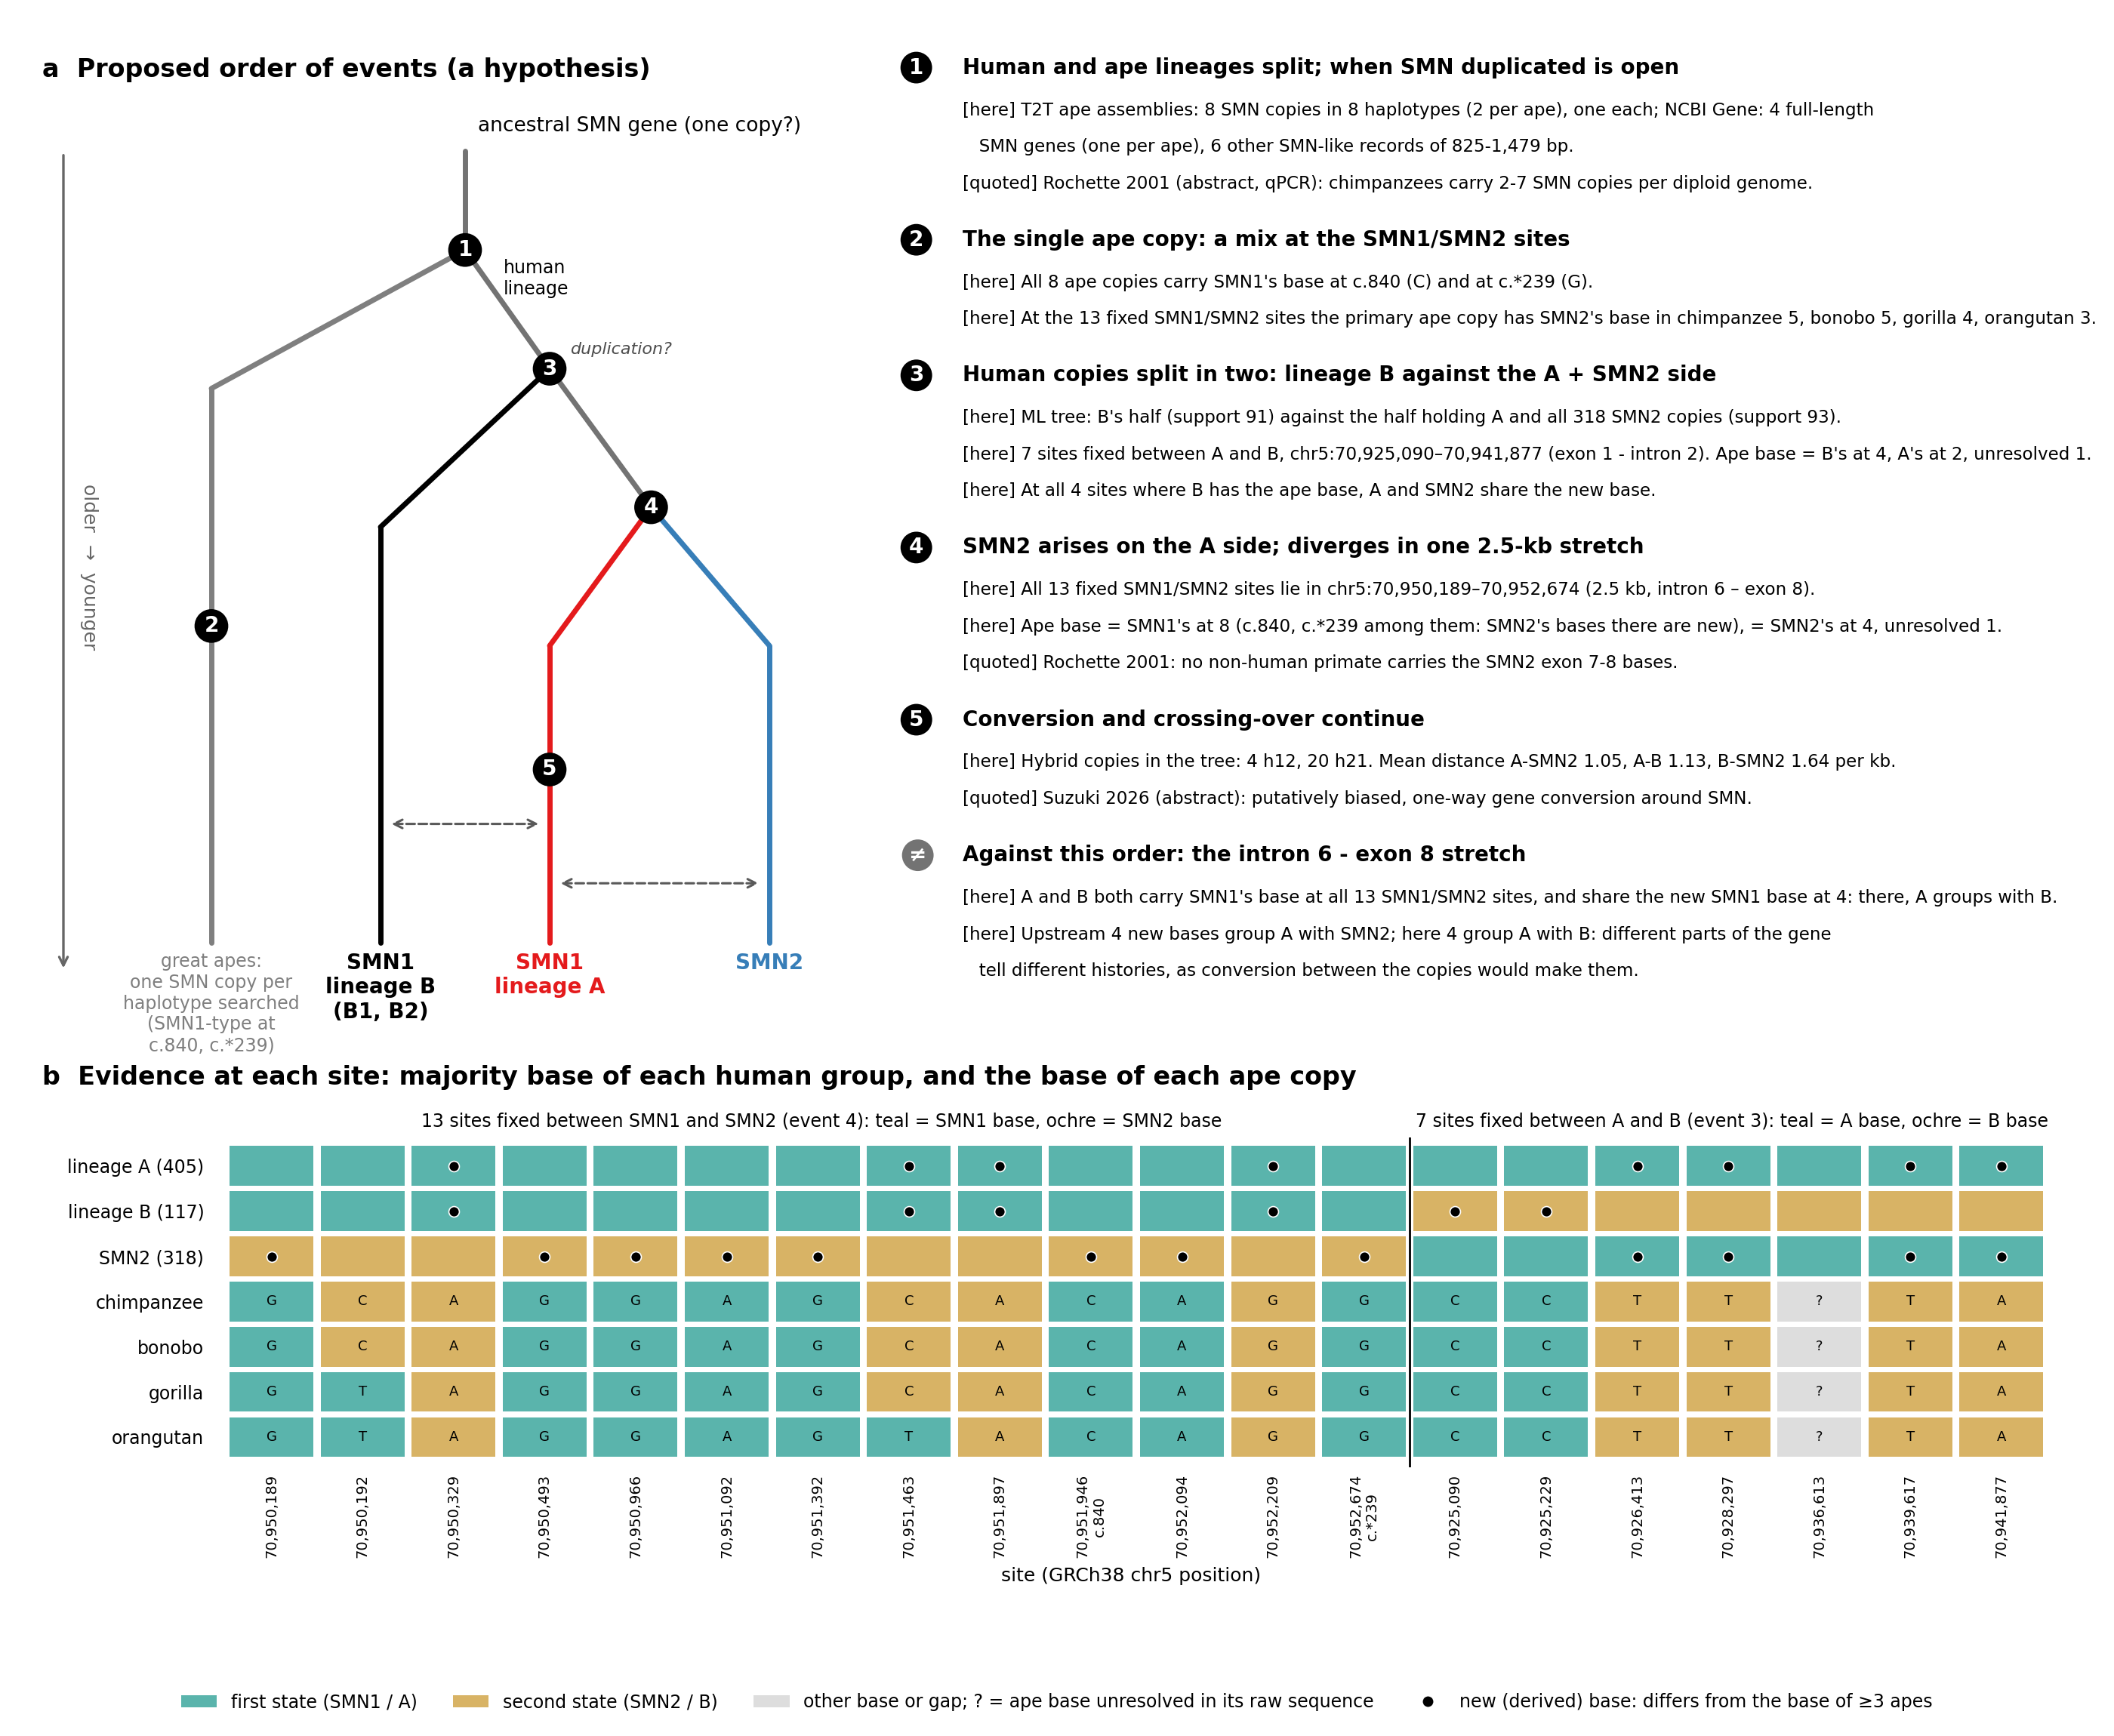
\includegraphics[width=\linewidth]{../figures/evolution_order.png}
\caption{A proposed order of events and the sites behind it. \textbf{a}, the order, with the evidence for each event
beside it: [here], computed in this study; [quoted], from a paper. \textbf{b}, each site where SMN1 and SMN2 (paralog sites)
or lineages A and B (A/B sites) are fixed for different bases: the majority base of lineage A, lineage B and SMN2 and
the base of each ape's copy, read from the ape's raw sequence (Methods; ?, a site no ape aligns across cleanly); teal, the first state (SMN1 or A); ochre, the second (SMN2 or B); a dot marks a human
group's base that differs from the base of at least three apes.}
\label{fig:evo}
\end{figure}

\section{Discussion}\label{m:disc}
\textbf{Assemblies give what dosage and reads leave out: where each copy sits.} Dosage assays count copies, and read
callers such as Paraphase sort them into haplogroups and phase variants within a gene~\cite{chen2023}; neither places
a copy on its chromosome. On the assemblies the order, orientation and repeat unit of every copy are read directly,
and that is how the common African two-copy SMN1 allele was seen to be a head-to-head pair of the B1 and B2
sub-lineages, and how the cenSMN arms were found to differ by whether they carry X, which goes with a split \emph{NAIP} where it is present, rather
than by more SMN copies. The structure that maps of the 1990s pieced together as one inverted duplication~\cite{lefebvre1995,campbell1997}
is, haplotype by haplotype, \arrTypes{} arrangements of SMN copies; on \palPair{} of the \palHaps{} haplotypes with
repeat units the copies sit on the two arms of a palindrome of large \RU{A} units, and on the other \palNoPair{} there is
no such palindrome.

\textbf{Structure and sequence vary together, and not simply.} One result is that a haplotype's
large-scale structure and the sequence of the SMN copies it carries are associated (Mantel correlation \mantelAll, $p\le$\,\mantelP),
yet the two trees built from them agree only loosely (cophenetic correlation \cophenetic). The link is not one rule but
a few bands, each joining a set of arrangements to one supported SMN1 clade, beside a bulk of haplotypes whose SMN1
copies fall in no supported clade of that size (Section~\ref{m:struct}). The S1-2 band holds no African-ancestry haplotype and none with the head-to-head \RU{A} pair (Supplementary Section~\ref{sec:bands}), and the SMN1
and SMN2 correlations remain when haplotypes are shuffled only within AFR and non-AFR, or within each of five continental groups, so shared ancestry alone does
not account for it, though within AFR the SMN1 correlation is weaker (Mantel Spearman $\rho=\mOneAFRR$, against \mOneR{} over all SMN1 copies). The tests treat haplotypes as
independent, and the structural distance also follows window length (Supplementary Section~\ref{sec:structseq}), so this is an
association: it suggests that structure and copy sequence share a history, and does not show how. The tree of Fig.~\ref{fig:mltree} shows the same link on the SMN2 side: a clade of \sTwoClN{} SMN2 copies (support \sTwoClSup\%) lies most often on ``2-~1-'' haplotypes (\sTwoClTwoMinusOneMinus{} of its \sTwoClN{} copies) and only \sTwoClAfr{} on an African-ancestry one, and \sTwoClWithSOneTwo{} of the \sTwoClHaps{} such haplotypes in the structure tree also carry an SMN1 copy of the S1-2 clade. The S1-2 band is thus a set of haplotypes whose SMN1 and SMN2 copies each belong to a clade of their own, a link of structure to the sequence of both copies that arises outside African ancestry and that the bulk of haplotypes does not show.

\textbf{How a palindrome could shape base changes is open.} On \palPair{} of \palHaps{} haplotypes the SMN copies lie one
on each arm of an inverted pair of repeat units, at distances from the axis that differ by a median of only
\palMirror{}~kb (Fig.~\ref{fig:palindrome}d), so the two copies of a haplotype sit at matching points of the mirror. Arms of the Y chromosome's
palindromes exchange sequence by gene conversion~\cite{rozen2003}, and in one of them the arms were estimated to
mutate more slowly than the spacer between them~\cite{bonito2021}.

At the amylase locus, which we studied earlier with
the same kind of assemblies and tools, nearly identical structures arose again and again on different haplotype
backgrounds~\cite{bolognini2024}, through recurrent non-allelic homologous recombination from an ancient three-copy
haplotype~\cite{yilmaz2024}, so there structure says little about the sequence it sits on; at 5q13
part of the cohort shows the opposite, structures that travel with one sequence clade.

Whether the palindrome acts on
base changes directly, through pairing and conversion between mirrored copies or through how often and where the
region rearranges, this study cannot say: it has no reads, no families and no mutation rates. It does say where to
look. If conversion between mirrored arms acts, the two copies of one haplotype should be closer in sequence than
copies at the same arm position on other haplotypes, conversion tracts should follow distance from the axis, and new
changes in trios sequenced with long reads should fall unevenly along the arms; each test is open to the data that
the next releases bring.

\textbf{For carrier testing, the lineage of a copy is a second axis beside its count.} A two-copy SMN1 allele in this
cohort's African-ancestry haplotypes usually carries lineage B (\ldTestBMulti{} of \ldTestMultiN{} such haplotypes),
most often as B1 at cenSMN and B2 at telSMN. Chen et al.\ proposed haplotype-based screening for silent carriers from
the S1-8 and S1-9 haplogroups~\cite{chen2023}; the sites that separate A from B, and the structural context, could serve
the same purpose and are open to testing in families. The marker \cpe{}, introduced as a tag of SMN1 duplication alleles~\cite{luo2014}, sits on \linBoneMk{} of the \linBone{} B1 copies but on \linBtwoMk{} of the \linBtwo{} B2 copies, which shows
why it misses part of the duplication alleles (Supplementary Section~\ref{sec:marker}). More broadly, a dosage assay reads one
number per person, while an assembly gives for each chromosome the copies' order, orientation, lineage and the repeat
units around them: the sites that separate A from B with no exception (\abPerfect, in the 5$'$ untranslated region and intron~1), the
B1-at-cenSMN, B2-at-telSMN pair, and the cenSMN arm type C0, which marks the structure cluster of the B1\,+\,B2 band. These are
candidate targets for assays that tell a two-copy chromosome from one copy on each, the case dosage misses; each
needs testing in families of known phase before use. The case is not rare in the cohort: \dosTwo{} of the \nHapsRes{} resolved haplotypes carry two or more \emph{SMN1} exon-7 copies (\dosTwoAfr{} of the \dosAfrHaps{} resolved AFR ones; the \mOneAFRN{} AFR haplotypes of the Mantel tests are these less the \dosAfrNoSmnOne{} with no \emph{SMN1} copy), \dosZero{} carry none, counted as a dosage assay counts them, by exon~7, so an h12 copy counts as \emph{SMN1} (whole \emph{SMN1} copies: \dosTwoCopy{} haplotypes with two or more, Supplementary Section~\ref{sec:bands}, and \dosNoCopy{} with none, Section~\ref{m:arr}; the \dosHOneTwoN{} haplotypes that change class between the two counts each carry an h12 copy, which has SMN1's base at c.840), and \dosPeopleTwo{} of the \dosPeople{} people with both haplotypes resolved have a two-copy chromosome. None of them is 2+0, but each two-copy chromosome passed on together with a deletion chromosome makes a silent carrier whom an exon-7 dosage test reads as two copies, a non-carrier.

\textbf{For reading reads, structure matters.} Reads from a person carrying B1 at cenSMN and B2 at telSMN come from two
SMN1 copies \gsBoneBtwo{} differences per kb apart over the gene body; knowing the arrangement and lineage of the
carrier's haplotypes tells a caller which copy a read belongs to. The same applies to \emph{NAIP}, whose copy number has been studied as a severity modifier (in one cohort it added nothing to \emph{SMN2} copy number~\cite{wadman2020}): a
haplotype whose cenSMN arm carries X has its \emph{NAIP} there split in two by Xi$'$ and X, so it carries one whole \emph{NAIP}
per window where a haplotype whose cenSMN arm lacks X carries two (\elNaipOneWholeCOne{} of \elCOne{} against \elNaipTwoWholeCZero{}
of \elCZero), a structural source of \emph{NAIP} copy-number differences distinct from the SMN unit, and one a dosage
assay of a single \emph{NAIP} exon would read differently depending on the exon.

\textbf{What the history suggests.} Most of SMN2's defining bases look derived (of the \evS{} sites, \evSancOne{} look derived, \evSancTwo{} ancestral and \evSunres{} unresolved), and in the gene-body tree, whose root the ape copies leave uncertain (Section~\ref{m:lineages}), the two supported halves separate an almost wholly African group (lineage B, with some h21 copies) from the rest, SMN2 included. At the A/B sites upstream, SMN2 carries A's base at all \evABtwoEqA, and A and SMN2 share
the newer base where the apes carry B's, while in the intron~6--exon~8 stretch A and B share newer SMN1 bases. With gene conversion active in the
region~\cite{campbell1997,vandersteege1996,suzuki2026}, a single tree is not a single history; trees of the intron~6--exon~8
stretch and of the rest of the gene, and more ape individuals, would test the order.

\section{Limitations}\label{m:lim}
\begin{itemize}
\item \textbf{Assembled bases only.} No read confirms a copy, its order or its orientation; an assembly error at a
copy-to-copy junction would change an arrangement and would show as reads that do not span it.
\item \textbf{Lineages from the same alignment.} A, B, B1 and B2 were cut from a maximum-likelihood tree of the same
alignment (supports \mlIsup, \mlIIsup, \mlBhSup{} and \mlEightSup); the node that joins B1 and B2 alone has support \mlBBjoinSup. Sites that separate
the lineages perfectly here may not in other samples.
\item \textbf{Copies are not independent.} Fisher, hypergeometric and permutation tests treat copies or haplotypes as independent;
copies of one haplotype, and haplotypes of one person, are not. Mantel tests shuffle haplotypes, some within AFR and non-AFR or within five continental groups; only the ancestry tests (Section~\ref{m:anc}) shuffle
whole people, keeping a person's two haplotypes together.
\item \textbf{Ancestry.} Lineage B is almost only in African-ancestry haplotypes, so its associations with arm and
structure cannot be tested elsewhere, and HPRC sampling is not proportional to populations.
\item \textbf{Structural distance.} PANGEA's bundle distance scores the whole window and follows window length; the
arrangement strings and the arm elements are the more direct description.
\item \textbf{Outgroups.} One copy per ape haplotype, from one individual per species, and \evS{} and \evAB{} sites;
the ape bases are read from one assembly each, one A/B site (\rdUnresSite) cannot be read in any ape, and gene conversion can make site patterns misleading.
\end{itemize}

\section{Methods}\label{m:methods}
\textbf{Data.} The HPRC release-2 assemblies~\cite{lucas2026} of \nPeopleAll{} people (\nHapsAll{} haplotypes) with GRCh38 and CHM13,
in an agc-rs archive (PANGEA's compressed sequence archive, from which any contig or stretch is extracted by name) indexed by PANGEA. The SMN window of each haplotype, its SMN copies and their classes, the gene
features in each window (\emph{SERF1}, \emph{NAIP}, \emph{GTF2H2}, \emph{GTF2H2C}, GTF2H2 family member~C; \emph{OCLN}, occludin) and the per-haplotype
tables come from a companion clinical study's pipeline at a fixed commit (\texttt{data/SOURCES.md}). The window is the contig stretch that a PANGEA query of the \wfQueryMb-Mb GRCh38 stretch chr5:\wfGStart--\wfGEnd{} against the release-2 index hits. All \wfN{} decomposed windows start within 2~kb of the query's start and \wfReachEnd{} reach its end (the other, \wfShortHap, ends \wfShortBp~bp short of it, still \wfShortTelKb~kb into single-copy sequence); every one begins and ends in bundles that occur only once in that window (the unique flank of Section~\ref{m:arms}), with at least \wfCenMin~kb (median \wfCenMed) of such single-copy sequence on the centromeric side and \wfTelMin~kb (median \wfTelMed) on the telomeric side (windows \wfLenMin--\wfLenMax~kb, median \wfLenMed; step~36). A copy is
counted when it lies away from contig ends and gaps and is either whole (all nine exons: 1, 2a, 2b and 3--8) or a
$\Delta$7--8 copy (exons 1--6, without 7 and 8). Of the \nCounted{} counted copies, \nAligned{} were aligned: the
\nJoined{} copy the pipeline joined from two pieces of one contig was left out. The \nDelLeftOut{} $\Delta$7--8 copies are in the alignment
(\nAlnRows{} rows) but are left out of the trees and distances (steps 05 and 07), which use the \nCopies{} whole copies. Copies are taken from every haplotype that carries one, resolved or not (\nCopiesUnres{} whole copies lie on \nCopiesUnresHaps{} haplotypes not resolved end to end); the structural comparisons use resolved haplotypes only.

\textbf{Structure.} The windows were decomposed together into principal bundles with \texttt{pangea cohort bundle decomp}
(\texttt{-w~48 -k~\dpCK{} -r~4 --min-span~\dpCSpan{} --min-branch-size~\dpCBranch{}}, bundle length cutoff and merge
distance \dpCCut~bp; \dpCSegs{} bundle segments of \dpCBids{} bundles; step~00) and into large repeat units with \texttt{pangea cohort bundle
repeat-units} at its default settings (PANGEA \verPangea; the algorithm is described in Supplementary Section~\ref{sec:compared}); the structural distance between two windows is the
\texttt{pangea cohort bundle dist} score on the top \setTopN{} bundles by span, which here is every one of the \dpCBids{} bundles (step~01). A finer decomposition (cutoff \dpFCut, merge distance \dpFMerge~bp, other settings default; \dpFBids{} bundles) is
used as a check (steps 01b, 28i and 37; every parameter of both in Supplementary Table~\ref{tab:decomp}).
\textbf{Arm elements.} On each haplotype with a head-to-head \RU{A} pair, every bundle segment is put on the cenSMN or
telSMN arm by its midpoint, measured from the axis and read outward with its strand as seen walking away from the axis
(step~28b). Named sets of bundles define the end of the core, Xi (both parts, Xi$'$ and Xi, told apart by bundle), S, Xd, E and the flank (Supplementary
Section~\ref{sec:palindrome}); the core runs from the axis to the end of the first end-of-core run beyond \elAstart~kb. An arm's
type is whether it carries Xd: C1 or C0 on the cenSMN arm (C0 carries none of Xi$'$, Xi, S and Xd), T1 or T0 on the telSMN
arm. Tandem arrays are PANGEA's \texttt{tandem-repeats} (units \trMinKb--\trMaxKb~kb) over every window (step~28); the spacer is
checked by sequence (step~28c). The copy's distance from the axis is split into the core stretch covered by the array's bundle and the rest
(step~28g; with the finer bundles, step~37). \emph{NAIP} pieces are placed on the exons of the RefSeq
transcript \nxTx, whose first bases map to GRCh38's \emph{NAIP} at the position the gene features give (step~28f). On haplotypes without the
pair, each S is read from its nearest SMN copy outward, by bundle id, without an axis (step~28h). For the apes, a 3-Mb
stretch around each ape copy is plotted against itself and against one human window (HG01099 mat) with PANGEA's shimmer
matcher, which marks every shimmer (a sparse pair of minimizers, PANGEA's indexing unit~\cite{chin2023}) the two sequences share (step~35), with the settings $w=24$, $k=48$, $r=2$ and a minimum span of 12. The measure of large repeats is the number of such dots more than 50~kb off the diagonal of a self dot plot, per Mb of sequence.

\textbf{Sequence.} Each counted copy, gene body with \setFlankKb~kb flanks on the SMN1-gene strand, was aligned with MAFFT
\verMafft{} FFT-NS-2~\cite{katoh2013} (step~02); distances use the \nGeneCols{} gene-body columns only and leave out
the \nDelLeftOut{} $\Delta$7--8 copies (Supplementary Section~\ref{sec:compared}). The
maximum-likelihood tree is IQ-TREE \verIqtree{}, \iqModel, \iqBoot{} ultrafast bootstraps~\cite{minh2020,hoang2018},
over the same columns with the four ape gene bodies (NCBI, T2T assemblies~\cite{yoo2025}) added by MAFFT
\texttt{--add --keeplength} (steps 03, 04a, 29). At the S and A/B sites of the history, each ape's base is then read from its raw primary sequence by local alignment of the 101-bp GRCh38 context (step~13c; Supplementary Section~\ref{sec:history}). Lineages A and B are the SMN1 copies of the two halves of the human
copies in this tree (support \mlIIsup{} and \mlIsup, below the 95 used for every other clade; Section~\ref{m:lineages}), and B1 and B2 the SMN1 copies of the two clades in B's half with support $\ge$95 that lie in no larger such clade: B1 the one that holds the h21 copies (\linBone{} SMN1 copies, of S1-9 and most S1-6, with \mlBhH{} h21 copies; support \mlBhSup), B2 the other (\linBtwo{} copies, support \mlEightSup); the \linBnone{} B copies outside both belong to neither (step~05); haplogroups are assigned copy by copy
(step~11): Chen et al.\ read their haplogroups off a neighbor-joining tree of SMN gene copies and Paraphase assigns a
new copy by its most similar representative sequence~\cite{chen2023}; here each SMN1 copy is given the haplogroup whose
listed single-base variants (their Table S6) it matches best, and check the result person by person against Paraphase's
calls (Supplementary Section~\ref{sec:chenhg}).

\textbf{Bands.} The structure tree (UPGMA, Sokal and Michener 1958, with optimal leaf order on bundle distance, over the \mlbHaps{} haplotypes
with an SMN1 copy) was cut into \setK{} clusters. On the sequence side each SMN1 copy was assigned to the smallest clade
of the maximum-likelihood tree with ultrafast-bootstrap support $\ge$\setMLsup{} that holds at least \setMLmin{} of
these SMN1 copies, or to the rest of the human clade; this gives \mlbClusters{} sequence clusters, and a haplotype's
sequence label is its copy's cluster, or the combination for several copies (\mlbLabels{} labels). Every structure
cluster by sequence label pair of five or more haplotypes was tested for excess overlap (hypergeometric test: the chance of at least that many shared haplotypes if the two groups were drawn at random; Bonferroni
over all pairs), and a band is a pair of at least \setMinOverlap{} haplotypes with corrected $p<\setAlpha$ (step~19b).
As a check, the support threshold (80, 90, 95) and clade size (5, 10, 20) were varied.

\textbf{Tests.} Mantel tests with Spearman correlation and \nPerm{} shuffles~\cite{mantel1967}; Fisher exact tests;
PERMANOVA and permutation tests that shuffle people; computed with NumPy~\cite{harris2020}, pandas and SciPy~\cite{virtanen2020},
figures with Matplotlib~\cite{matplotlib}. Seeds are fixed and outputs sorted.

\textbf{Numbers and figures.} \texttt{scripts/run\_all.sh} runs every numbered step in \texttt{scripts/} in order, 00 to 43 (with the lettered steps 01b, 04a, 13b, 13c, 19b, 19c, 19d, 23b, 28b--28j and 34b; step 28j is two scripts: \texttt{28j\_fig5.py} draws the band figure, Supplementary Fig.~\ref{fig:tangclus}, with the arm-type strips of 28b, and \texttt{28j\_a\_unit\_length.py} measures the \RU{A} units), \texttt{41\_provenance.py}, and \texttt{scripts/40\_numbers.py},
which writes every number of this document as a macro with the script line and input files that produce it
(\texttt{note/numbers.json}); Supplementary Section~\ref{sec:provenance} shows how the data flow through the steps
and where each number comes from. The example haplotypes of Fig.~\ref{fig:locus} are chosen by rule: among haplotypes whose two arms
both have their type's commonest layout, the two-copy ``2-~1+'' haplotype of form C1|T0 (a) and the ``1-~1+'' B1+B2
haplotype of form C0|T1 (b) nearest the medians of arm length and mirror difference.

\section*{Availability, contributions and use of AI}
Code, result tables and this document's sources are in the project repository, \url{https://github.com/Diploid-Genomics-Inc/smn-repeat-structure}. All PANGEA steps (\texttt{pangea} and \texttt{agc-rs}) used version 0.27.0 (build 56818da6); a macOS (Apple silicon) binary of this version will be released with the repository [placeholder: binary release URL and SHA-256]. The HPRC release-2
assemblies are public; the list of the contigs used, with their GenBank accessions and the window taken from each (\texttt{data/hprc\_r2\_contigs\_used.tsv}), is available in the same repository. \textbf{Contributions.} C.S.C.: conceptualization, directing the computation and experiments, choosing the research
direction, reading and revision. PANGEA Strata (Research Intelligence Development Environment): managing and recording the research process
with the LLM, and tracking the artifacts for verification and validation. Claude (Opus 5.5, Anthropic): LLM; drafting,
coding for the analysis and diagrams, testing, and advice on analysis approaches.

% Written by the tex module's build_pdf from references.toml: edit the records, not this file.
\providecommand{\url}[1]{\texttt{#1}}\providecommand{\nolinkurl}[1]{\texttt{#1}}
\begin{thebibliography}{46}
\bibitem{lefebvre1995} Lefebvre S, Bürglen L, Reboullet S, Clermont O, Burlet P, Viollet L, et al. Identification and characterization of a spinal muscular atrophy-determining gene. Cell 1995;80(1):155-65. doi:\nolinkurl{10.1016/0092-8674(95)90460-3}
\bibitem{lorson1999} Lorson CL, Hahnen E, Androphy EJ, Wirth B. A single nucleotide in the SMN gene regulates splicing and is responsible for spinal muscular atrophy. Proc Natl Acad Sci U S A 1999;96(11):6307-11. doi:\nolinkurl{10.1073/pnas.96.11.6307}
\bibitem{monani1999} Monani UR, Lorson CL, Parsons DW, Prior TW, Androphy EJ, Burghes AH, et al. A single nucleotide difference that alters splicing patterns distinguishes the SMA gene SMN1 from the copy gene SMN2. Hum Mol Genet 1999;8(7):1177-83. doi:\nolinkurl{10.1093/hmg/8.7.1177}
\bibitem{mercuri2022} Mercuri E, Sumner CJ, Muntoni F, Darras BT, Finkel RS. Spinal muscular atrophy. Nat Rev Dis Primers 2022;8(1):52. doi:\nolinkurl{10.1038/s41572-022-00380-8}
\bibitem{finkel2017} Finkel RS, Mercuri E, Darras BT, Connolly AM, Kuntz NL, Kirschner J, et al. Nusinersen versus Sham Control in Infantile-Onset Spinal Muscular Atrophy. N Engl J Med 2017;377(18):1723-32. doi:\nolinkurl{10.1056/NEJMoa1702752}
\bibitem{mendell2017} Mendell JR, Al-Zaidy S, Shell R, Arnold WD, Rodino-Klapac LR, Prior TW, et al. Single-Dose Gene-Replacement Therapy for Spinal Muscular Atrophy. N Engl J Med 2017;377(18):1713-22. doi:\nolinkurl{10.1056/NEJMoa1706198}
\bibitem{prior2008} Prior TW. Carrier screening for spinal muscular atrophy. Genet Med 2008;10(11):840-2. doi:\nolinkurl{10.1097/GIM.0b013e318188d069}
\bibitem{hendrickson2009} Hendrickson BC, Donohoe C, Akmaev VR, Sugarman EA, Labrousse P, Boguslavskiy L, et al. Differences in SMN1 allele frequencies among ethnic groups within North America. J Med Genet 2009;46(9):641-4. doi:\nolinkurl{10.1136/jmg.2009.066969}
\bibitem{sugarman2012} Sugarman EA, Nagan N, Zhu H, Akmaev VR, Zhou Z, Rohlfs EM, et al. Pan-ethnic carrier screening and prenatal diagnosis for spinal muscular atrophy: clinical laboratory analysis of >72,400 specimens. Eur J Hum Genet 2012;20(1):27-32. doi:\nolinkurl{10.1038/ejhg.2011.134}
\bibitem{luo2014} Luo M, Liu L, Peter I, Zhu J, Scott SA, Zhao G, et al. An Ashkenazi Jewish SMN1 haplotype specific to duplication alleles improves pan-ethnic carrier screening for spinal muscular atrophy. Genet Med 2014;16(2):149-56. doi:\nolinkurl{10.1038/gim.2013.84}
\bibitem{feng2017} Feng Y, Ge X, Meng L, Scull J, Li J, Tian X, et al. The next generation of population-based spinal muscular atrophy carrier screening: comprehensive pan-ethnic SMN1 copy-number and sequence variant analysis by massively parallel sequencing. Genet Med 2017;19(8):936-44. doi:\nolinkurl{10.1038/gim.2016.215}
\bibitem{milligan2021} Milligan JN, Larson JL, Filipovic-Sadic S, Laosinchai-Wolf W, Huang YW, Ko TM, et al. Multisite Evaluation and Validation of a Sensitive Diagnostic and Screening System for Spinal Muscular Atrophy that Reports SMN1 and SMN2 Copy Number, along with Disease Modifier and Gene Duplication Variants. J Mol Diagn 2021;23(6):753-64. doi:\nolinkurl{10.1016/j.jmoldx.2021.03.004}
\bibitem{mikhalchuk2025} Mikhalchuk K, Polyakov A, Zabnenkova VV, Ismagilova O, Shchagina O. Exploring the Prevalence of SMN1 Duplication and Deletion in Russia and Its Impact on Carrier Screening. Int J Mol Sci 2025;26(5). doi:\nolinkurl{10.3390/ijms26051984}
\bibitem{chen2020} Chen X, Sanchis-Juan A, French CE, Connell AJ, Delon I, Kingsbury Z, et al. Spinal muscular atrophy diagnosis and carrier screening from genome sequencing data. Genet Med 2020;22(5):945-53. doi:\nolinkurl{10.1038/s41436-020-0754-0}
\bibitem{chen2023} Chen X, Harting J, Farrow E, Thiffault I, Kasperaviciute D, Hoischen A, et al. Comprehensive SMN1 and SMN2 profiling for spinal muscular atrophy analysis using long-read PacBio HiFi sequencing. Am J Hum Genet 2023;110(2):240-50. doi:\nolinkurl{10.1016/j.ajhg.2023.01.001}
\bibitem{brzustowicz1990} Brzustowicz LM, Lehner T, Castilla LH, Penchaszadeh GK, Wilhelmsen KC, Daniels R, et al. Genetic mapping of chronic childhood-onset spinal muscular atrophy to chromosome 5q11.2-13.3. Nature 1990;344(6266):540-1. doi:\nolinkurl{10.1038/344540a0}
\bibitem{melki1990} Melki J, Abdelhak S, Sheth P, Bachelot MF, Burlet P, Marcadet A, et al. Gene for chronic proximal spinal muscular atrophies maps to chromosome 5q. Nature 1990;344(6268):767-8. doi:\nolinkurl{10.1038/344767a0}
\bibitem{gilliam1990} Gilliam TC, Brzustowicz LM, Castilla LH, Lehner T, Penchaszadeh GK, Daniels RJ, et al. Genetic homogeneity between acute and chronic forms of spinal muscular atrophy. Nature 1990;345(6278):823-5. doi:\nolinkurl{10.1038/345823a0}
\bibitem{roy1995} Roy N, Mahadevan MS, McLean M, Shutler G, Yaraghi Z, Farahani R, et al. The gene for neuronal apoptosis inhibitory protein is partially deleted in individuals with spinal muscular atrophy. Cell 1995;80(1):167-78. doi:\nolinkurl{10.1016/0092-8674(95)90461-1}
\bibitem{burglen1997} Bürglen L, Seroz T, Miniou P, Lefebvre S, Burlet P, Munnich A, et al. The gene encoding p44, a subunit of the transcription factor TFIIH, is involved in large-scale deletions associated with Werdnig-Hoffmann disease. Am J Hum Genet 1997;60(1):72-9.
\bibitem{campbell1997} Campbell L, Potter A, Ignatius J, Dubowitz V, Davies K. Genomic variation and gene conversion in spinal muscular atrophy: implications for disease process and clinical phenotype. Am J Hum Genet 1997;61(1):40-50. doi:\nolinkurl{10.1086/513886}
\bibitem{vandersteege1996} van der Steege G, Grootscholten PM, Cobben JM, Zappata S, Scheffer H, den Dunnen JT, et al. Apparent gene conversions involving the SMN gene in the region of the spinal muscular atrophy locus on chromosome 5. Am J Hum Genet 1996;59(4):834-8.
\bibitem{vorster2020} Vorster E, Essop FB, Rodda JL, Krause A. Spinal Muscular Atrophy in the Black South African Population: A Matter of Rearrangement?. Front Genet 2020;11:54. doi:\nolinkurl{10.3389/fgene.2020.00054}
\bibitem{wadman2020} Wadman RI, Jansen MD, Stam M, Wijngaarde CA, Curial CAD, Medic J, et al. Intragenic and structural variation in the SMN locus and clinical variability in spinal muscular atrophy. Brain Commun 2020;2(2):fcaa075. doi:\nolinkurl{10.1093/braincomms/fcaa075}
\bibitem{berzal2026} Berzal-Serrano A, González-Alvaredo S, Lesende I, Carretero-Vilarroig L, Jaijo T, Onsurbe I, et al. Multimodal characterisation of the SMN locus in SMA: copy number quantification and hybrid gene identification. NPJ Genom Med 2026;11(1). doi:\nolinkurl{10.1038/s41525-026-00579-8}
\bibitem{liao2023} Liao WW, Asri M, Ebler J, Doerr D, Haukness M, Hickey G, et al. A draft human pangenome reference. Nature 2023;617(7960):312-24. doi:\nolinkurl{10.1038/s41586-023-05896-x}
\bibitem{lucas2026} Lucas JK, Hebbar P, Liao W, Macias-Velasco JF, Novak AM, Asri M, et al. HPRC2: A human pangenome reference with near-complete coverage of common genetic variation. bioRxiv (preprint) 2026. doi:\nolinkurl{10.64898/2026.07.21.739710}
\bibitem{logsdon2025} Logsdon GA, Ebert P, Audano PA, Loftus M, Porubsky D, Ebler J, et al. Complex genetic variation in nearly complete human genomes. Nature 2025;644(8076):430-41. doi:\nolinkurl{10.1038/s41586-025-09140-6}
\bibitem{suzuki2026} Suzuki Y, Owa C, Kobayashi H, Nakabayashi R, McNulty B, Violich I, et al. Accessing medically relevant complex regions with a pangenome graph of 20 near-complete Japanese haplotypes. Nat Commun 2026;17(1). doi:\nolinkurl{10.1038/s41467-026-73461-x}
\bibitem{zwartkruis2025} Zwartkruis MM, Elferink MG, Gommers D, Signoria I, Blasco-Pérez L, Costa-Roger M, et al. Long-read sequencing identifies copy-specific markers of SMN gene conversion in spinal muscular atrophy. Genome Med 2025;17(1):26. doi:\nolinkurl{10.1186/s13073-025-01448-2}
\bibitem{hickey2024} Hickey G, Monlong J, Ebler J, Novak AM, Eizenga JM, Gao Y, et al. Pangenome graph construction from genome alignments with Minigraph-Cactus. Nat Biotechnol 2024;42(4):663-73. doi:\nolinkurl{10.1038/s41587-023-01793-w}
\bibitem{chin2023} Chin CS, Behera S, Khalak A, Sedlazeck FJ, Sudmant PH, Wagner J, et al. Multiscale analysis of pangenomes enables improved representation of genomic diversity for repetitive and clinically relevant genes. Nat Methods 2023;20(8):1213-21. doi:\nolinkurl{10.1038/s41592-023-01914-y}
\bibitem{anderson2001} Anderson MJ. A new method for non-parametric multivariate analysis of variance. Austral Ecology 2001;26:32-46. doi:\nolinkurl{10.1111/j.1442-9993.2001.01070.pp.x}
\bibitem{yoo2025} Yoo D, Rhie A, Hebbar P, Antonacci F, Logsdon GA, Solar SJ, et al. Complete sequencing of ape genomes. Nature 2025;641(8062):401-18. doi:\nolinkurl{10.1038/s41586-025-08816-3}
\bibitem{rochette2001} Rochette CF, Gilbert N, Simard LR. SMN gene duplication and the emergence of the SMN2 gene occurred in distinct hominids: SMN2 is unique to Homo sapiens. Hum Genet 2001;108(3):255-66. doi:\nolinkurl{10.1007/s004390100473}
\bibitem{rozen2003} Rozen S, Skaletsky H, Marszalek JD, Minx PJ, Cordum HS, Waterston RH, et al. Abundant gene conversion between arms of palindromes in human and ape Y chromosomes. Nature 2003;423(6942):873-6. doi:\nolinkurl{10.1038/nature01723}
\bibitem{bonito2021} Bonito M, D'Atanasio E, Ravasini F, Cariati S, Finocchio A, Novelletto A, et al. New insights into the evolution of human Y chromosome palindromes through mutation and gene conversion. Hum Mol Genet 2021;30(23):2272-85. doi:\nolinkurl{10.1093/hmg/ddab189}
\bibitem{bolognini2024} Bolognini D, Halgren A, Lou RN, Raveane A, Rocha JL, Guarracino A, et al. Recurrent evolution and selection shape structural diversity at the amylase locus. Nature 2024;634(8034):617-25. doi:\nolinkurl{10.1038/s41586-024-07911-1}
\bibitem{yilmaz2024} Yilmaz F, Karageorgiou C, Kim K, Pajic P, Scheer K, Beck CR, et al. Reconstruction of the human amylase locus reveals ancient duplications seeding modern-day variation. Science 2024;386(6724):eadn0609. doi:\nolinkurl{10.1126/science.adn0609}
\bibitem{katoh2013} Katoh K, Standley DM. MAFFT multiple sequence alignment software version 7: improvements in performance and usability. Mol Biol Evol 2013;30(4):772-80. doi:\nolinkurl{10.1093/molbev/mst010}
\bibitem{minh2020} Minh BQ, Schmidt HA, Chernomor O, Schrempf D, Woodhams MD, von Haeseler A, et al. IQ-TREE 2: New Models and Efficient Methods for Phylogenetic Inference in the Genomic Era. Mol Biol Evol 2020;37(5):1530-4. doi:\nolinkurl{10.1093/molbev/msaa015}
\bibitem{hoang2018} Hoang DT, Chernomor O, von Haeseler A, Minh BQ, Vinh LS. UFBoot2: Improving the Ultrafast Bootstrap Approximation. Mol Biol Evol 2018;35(2):518-22. doi:\nolinkurl{10.1093/molbev/msx281}
\bibitem{mantel1967} Mantel N. The detection of disease clustering and a generalized regression approach. Cancer Res 1967;27(2):209-20.
\bibitem{harris2020} Harris CR, Millman KJ, van der Walt SJ, Gommers R, Virtanen P, Cournapeau D, et al. Array programming with NumPy. Nature 2020;585(7825):357-62. doi:\nolinkurl{10.1038/s41586-020-2649-2}
\bibitem{virtanen2020} Virtanen P, Gommers R, Oliphant TE, Haberland M, Reddy T, Cournapeau D, et al. SciPy 1.0: fundamental algorithms for scientific computing in Python. Nat Methods 2020;17(3):261-72. doi:\nolinkurl{10.1038/s41592-019-0686-2}
\bibitem{matplotlib} The Matplotlib Development Team. Matplotlib: visualization with Python [computer program]. 2025 [cited 2026-11-14]. Available from: \url{https://matplotlib.org}
\end{thebibliography}


\clearpage
\appendix
\renewcommand{\thesection}{S\arabic{section}}
\renewcommand{\thefigure}{S\arabic{figure}}
\renewcommand{\thetable}{S\arabic{table}}
\setcounter{figure}{0}\setcounter{table}{0}
\begin{center}\Large Supplementary information\end{center}
% Supplementary text. First converted 2026-11-14 from explore/structure_vs_sequence/doc/structure_vs_sequence.tex
% (commit 25bae39 lineage) by scratch/make_supp.py, then edited here as source.
\section{Definitions: copies, arrangements, alignment columns and distances}\label{sec:compared}
\textbf{Structure} of a haplotype is the composition and order of the principal bundles (sequence blocks shared
across haplotypes) along its whole SMN window, as decomposed by PANGEA, the successor of PGR-TK~\cite{chin2023}.
The \emph{structural distance} between two windows is the score of \texttt{pangea cohort bundle dist} (0 =
same bundles in the same order). It reflects the large repeat units, hundreds of kilobases long, that carry the SMN copies, not the SMN genes themselves.

\textbf{Which haplotypes each comparison uses.} Of the \nHapsAll{} haplotypes, \nHapsRes{} are \emph{resolved} (the SMN region on one contig). Two different sets of the same size come from them: the \nHapsResSMNone{} resolved haplotypes that carry an SMN1 copy (\nHapsResNoSMNone{} carry none) and the \palHaps{} whose window has repeat units (\nHapsNoUnits{} have none). Structure is compared with SMN1 sequence (Mantel tests by lineage, the two trees, the bands) on \mlbHaps{} haplotypes: the \nHapsResSMNone{} resolved haplotypes with an SMN1 copy, and GRCh38 and CHM13; the SMN2-only Mantel test uses the \mTwoN{} haplotypes with an SMN2 copy; the all-copy Mantel test uses all \nHapsRes{} resolved haplotypes with the two references (\setAllCopy); the palindrome and arm results use the \palHaps{} with units; the ancestry tests use the \anHaps{} resolved haplotypes in the five continental groups, leaving out \setNoLab{} without a population label and \setAsl{} from ASL.

\textbf{Sequence} is the gene body of each counted SMN copy (SMN1, SMN2 and the hybrids h12 and h21, read from the
assemblies by the study's pipeline).

\textbf{Repeat units and their families (Table~\ref{tab:unitfam}; Fig.~\ref{fig:ruAlgo}).} A haplotype's \emph{window}
is the stretch of its contig that a PANGEA query of the GRCh38 stretch chr5:\wfGStart--\wfGEnd{} hits; every window
begins and ends in bundles that occur once in it (Fig.~\ref{fig:ruAlgo}a; Methods). PANGEA's \texttt{repeat-units}
(version 0.27.0, default settings) takes a window's bundle segments in order, each with a bundle id, a strand, a start and
an end, and works in six steps (Fig.~\ref{fig:ruAlgo}b,c):
\begin{enumerate}
\item \emph{Self-match.} Two segments with the same bundle id match: directly when on the same strand, inverted when on
opposite strands. This is a dot plot of the window against itself, in bundles.
\item \emph{Chains.} Matches are joined along diagonals (anti-diagonals for inverted matches). A step may skip up to
\ufMaxGap{} segments on both copies, or up to \ufMaxIndel{} on one copy (an indel), but not segments of the step's own
bundle, which would be another copy in a tandem array. A chain scores the bases of its matched segments, less, at each
step, a quarter of the difference between the bases skipped on the two copies.
\item \emph{Palindrome centers.} Where segments mirror each other outward from a point, on each side over at least the
minimum unit span and \ufMinMatch{} mirrored pairs, the point is a palindrome center; chains that cross it are cut there.
\item \emph{Tandem arrays.} A chain whose two copies overlap, with at least 90\% of its matches at one offset and at
least 2.5 units, is a tandem array; copies that fall in it are snapped to whole units.
\item \emph{Copies.} Chains are taken best first. A chain adds its two copies when they do not overlap, hold at least
\ufMinMatch{} matched segments and the shorter spans the minimum unit span (the median window span divided by 50, held
within 5--40~kb; \ufAutoKb{}~kb here). A copy that overlaps a known copy by half or more is that copy; otherwise it keeps
only the segments no earlier copy holds. Copies found by one chain are linked into one repeat.
\item \emph{Families.} A copy's \emph{bundle content} is the number of bases of each bundle id within its span, strand
ignored; a family's mean content is that number averaged over its members. Over all windows, copies are taken from the
longest. Each joins the family most similar to it by bp-weighted Jaccard similarity, the sum over bundle ids of the
smaller of the copy's and the family's bases divided by the sum of the larger, if that similarity is at least \ufJac{}
(a Jaccard distance of at most 1$-$\ufJac); otherwise it founds a family. The elements compared are thus bases, each labeled only by its bundle id: two copies share a base of bundle~$b$ wherever both hold one, whatever its exact sequence, and no k-mers or base-level alignment enter. Families are lettered by the bases they
cover, the most first.
\end{enumerate}
Over the \ufWindows{} windows this gives \ufOcc{} occurrences in \ufFams{} families (\ufInv{} inverted and \ufDir{}
direct relative to another occurrence; the shortest unit is \ufShortKb~kb, one of \ufBelowN{} \RU{\ufBelowFam} units
below the minimum span). Table~\ref{tab:unitfam} lists the \ufBig{} families with ten or more occurrences (the other
\ufSmallFams{} hold \ufSmallOcc). A family is defined by its bundle content, not by one fixed sequence; its \emph{core
bundles}, present in at least 90\% of its occurrences, are listed with the share of the family's bases they cover.

\begin{figure}[!htbp]\centering
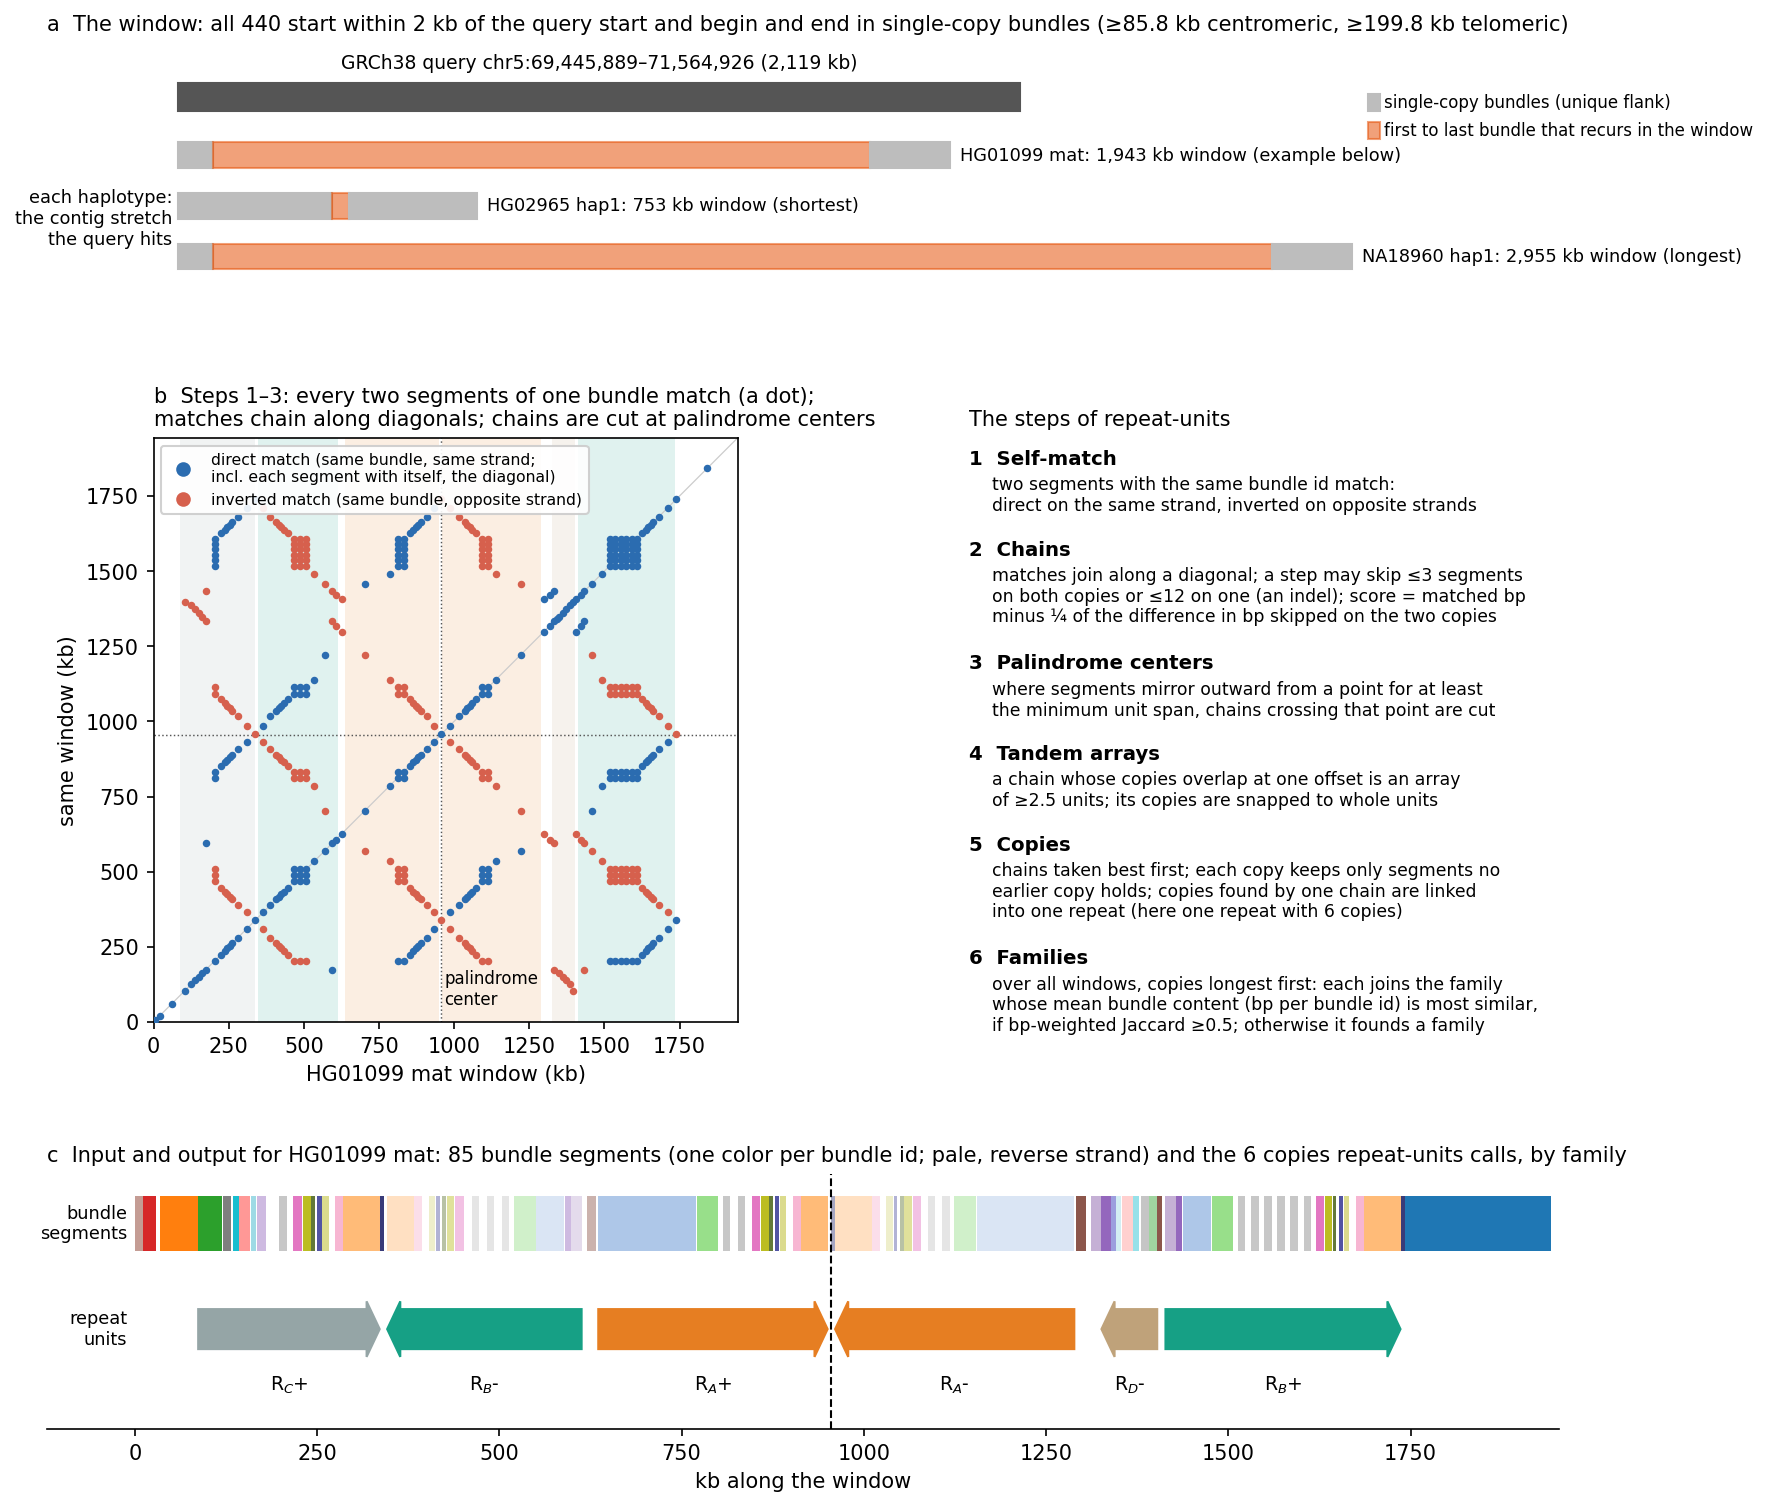
\includegraphics[width=\linewidth]{../figures/repeat_units_algo.png}
\caption{How a window is taken and how \texttt{repeat-units} turns it into repeat units. \textbf{a}, the window: the
stretch of each haplotype's contig hit by the GRCh38 query, drawn to scale for the example haplotype of b and c and for
the shortest and longest windows; gray, the single-copy bundles at each end; orange, from the first to the last bundle
that recurs in the window. \textbf{b}, the self-match of \ruaEx{} in bundles (step~1): one dot per pair of segments of
the same bundle, blue direct and red inverted; chains follow the lines of dots (step~2); the dashed lines mark the
palindrome center at which chains are cut (step~3); shading, the copies called, colored by family. Steps 1--6 are
summarized beside it. \textbf{c}, the input (\ruaSeg{} bundle segments, one color per bundle id, pale on the reverse
strand) and the output (\ruaUnits{} copies, by family and strand) for the same window. Drawn by
\texttt{scripts/39\_repeat\_units\_diagram.py}.}\label{fig:ruAlgo}
\end{figure}

\textbf{Units do not overlap in position, but they may be homologous to each other.} In a window no two units share more than the 55 bases ($k$) that neighboring bundle segments can share
(\ufPosOv{} pairs overlap by more; the ends of \ufKmerOv{} neighboring pairs touch by 1--55 bases; \ufOcc{} occurrences): \texttt{repeat-units} keeps the span of a copy found by a
better-scoring chain and gives a copy found later only the bundle segments that no known copy holds, and a final guard
splits any remaining overlap at its middle (steps 2 and 5 of the algorithm above). A family, however, is
defined by similarity of bundle content (bp-weighted Jaccard similarity at least \ufJac{} to the family's mean content; step~6), not by bundles of its own, so the
same bundles, and so the same sequence, recur in units of different families: the core bundles of \ufInA{} all lie
within \RU{A}'s (\RU{B} has exactly \RU{A}'s \ufABshared{} core bundles; see below), \ufPairsShare{} of the \ufPairs{} pairs of families in
Table~\ref{tab:unitfam} share at least one core bundle, and \ufBidsMulti{} of the \ufBids{} bundle ids found in units (an id counts when one of its segments lies within a unit's span)
appear in units of two or more families. Families \RU{A} and \RU{B} are the clearest case. Read in each unit's own orientation, both hold the same \ufABshared{} core
bundles in the same order and orientation (\ufABorder; in \ufAinOrd{} of \ufAn{} \RU{A} and \ufBinOrd{} of \ufBn{} \RU{B} units).
They differ in how much of two of them a unit holds and in what lies beside them: bundle~1 covers a median \ufAbOneA{} kb
in an \RU{A} unit against \ufAbOneB{} kb in an \RU{B} unit, the array bundle~15 \ufAbArrA{} against \ufAbArrB{} kb (the other
eight core bundles differ by at most \ufAbOtherMax{} kb), \ufBstartK{} \RU{B} units and no \RU{A} unit open with bundles 9+~8+,
and \ufAtenM{} \RU{A} units and no \RU{B} unit carry bundle 10$-$ before the core. In arm elements \RU{A} is mostly the core
(\feACore{} of its bases) and \RU{B} mostly Xi$'$ and Xi (\feBXi; Table~\ref{tab:unitfamel}): \RU{B} is the inverted copy of the core's
inner part, so the two families are one sequence seen from the two sides of the palindrome, cut at different places.

\textbf{Why \RU{A} and \RU{B} are two families although they share their core bundles.} The family rule (step~6
above) decides it, and it weighs bases, not bundle ids. \RU{A} was founded by the longest copy, \ufAfoundKb~kb. The
first \RU{B} copy, \ufBfoundKb~kb, scored \ufBfoundSim{} against \RU{A}'s mean content at that point, below the \ufJac{}
needed to join, and so founded a family of its own; each later copy joined the nearer of the two. The bases that set
them apart are those of two core bundles: the mean \RU{A} unit holds \ufMeanOneA~kb of bundle~1 against \ufMeanOneB~kb in
an \RU{B} unit, and \ufMeanArrA~kb of the array bundle~15 against \ufMeanArrB~kb. Every \RU{B} unit (\ufBcloser{} of
\ufBn) and \ufAcloser{} of the \ufAn{} \RU{A} units lie nearer their own family's final mean than the other's (median
similarity to their own mean \ufAownSim{} and \ufBownSim). The two families are nevertheless close: their final mean
contents have a similarity of \ufMeansSim, above the threshold, and \ufBgeThr{} of the \ufBn{} \RU{B} units would pass it
against \RU{A}'s final mean (median \ufBvsASim). \RU{A} and \RU{B} are thus two neighboring clusters of the same
sequence; where the line between them falls depends on the order in which the rule met the copies and on the
threshold, and taken in another order the two could have formed one family.

\textbf{How alike the families are in sequence.} The family rule compares bundle content. To compare sequence we took up
to \fsN{} units of each family with at least \fsMinOcc{} donor occurrences (\fsFams{} families, \fsUnits{} units, one per
haplotype) and, for every two units from different haplotypes (\fsPairs{} pairs), matched their shimmers (w24, k48,
r2) and took the Jaccard similarity of the two units' shimmer sets (shared over union; Fig.~\ref{fig:famshim}). Units
of one family are \fsJDiagLo--\fsJDiagHi{} alike, and \RU{A} and \RU{B} are the most alike pair of different families
(\fsJAB, against at most \fsJOtherMax{} for any other pair; \RU{B} with itself \fsJBB). Much of the spread within a
family is length: counted over the shorter unit's shimmers, units of one family are \fsODiagLo--\fsODiagHi{} alike
(\RU{B} \fsOBB), the shorter unit lying largely within the longer. Counted by direction, \fsCBA{} of an \RU{B} unit's
shimmers are found in an \RU{A} unit and \fsCAB{} the other way, so \RU{B} is largely a part of \RU{A}'s sequence;
\RU{D} lies largely within \RU{C} (\fsCDC{} against \fsCCD), and against \RU{A} or \RU{B} every median is at most
\fsDABMax. Shimmer positions are matched without their order, and the samples of \RU{F} and \RU{J} are small. Drawn by \texttt{43\_family\_shimmer.py}.

\begin{figure}[htbp]
\centering
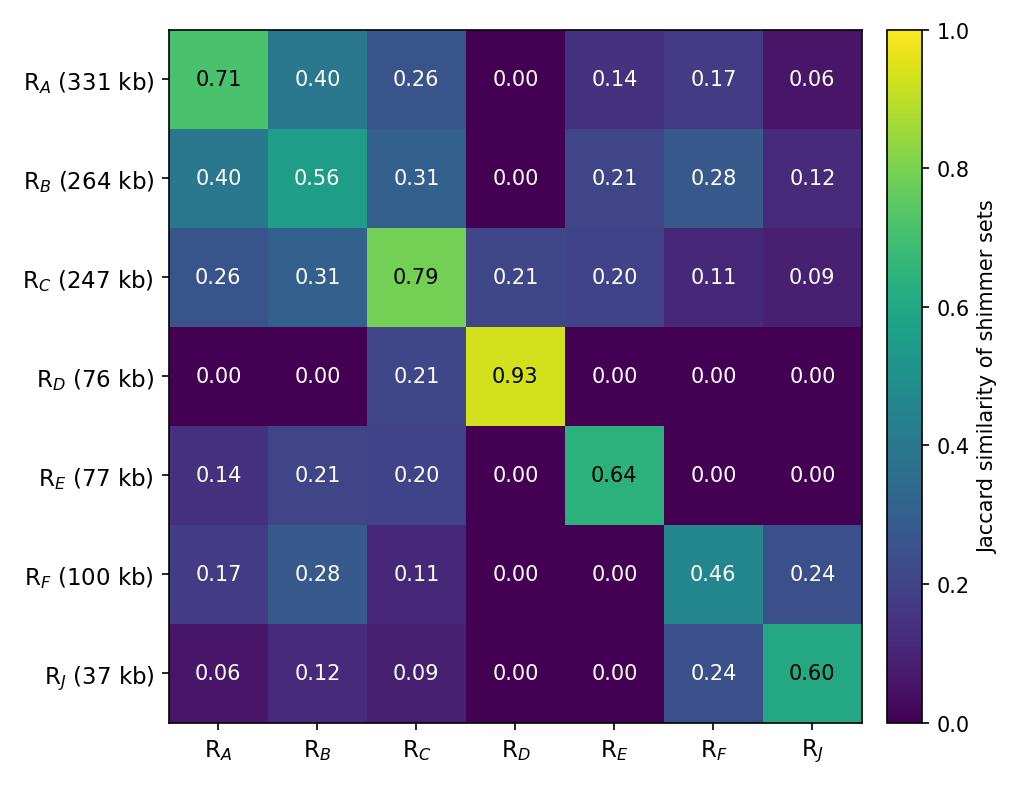
\includegraphics[width=0.62\linewidth]{../figures/family_shimmer.png}
\caption{Sequence similarity between repeat-unit families: Jaccard similarity of two units' shimmer sets (shared over
union), the median over pairs of units from different haplotypes (up to \fsN{} units per family, one per haplotype;
\fsPairs{} pairs). Row labels give the median length of the sampled units. Drawn by
\texttt{43\_family\_shimmer.py}.}
\label{fig:famshim}
\end{figure}

Which family a stretch of sequence is labeled with depends on
which chain claimed it first and where that chain stopped. The arms are compared by their elements, not their units
(Section~\ref{sec:palindrome}, Fig.~\ref{fig:palindrome}). The table is written by \texttt{33\_unit\_families.py} and \texttt{40\_numbers.py}.

\textbf{Why unit boundaries are not unique.} The region is built of nested repeats, in both orientations: the core and its inverted copy across the axis (the \RU{A}+\,\RU{A}$-$ pair), beyond the core an inverted copy of it, split by a tandem array into Xi$'$ and Xi, and Xi again in the core's orientation (Xd), with the spacer S at the center of each inverted pair (Section~\ref{sec:palindrome}, Table~\ref{tab:elements}). Read outward from the axis, the same bundles therefore recur several times, at different distances and in both orientations, and a repeat finder has to choose which copies to pair and where each copy ends. PANGEA's \texttt{repeat-units} pairs them from the best-scoring chain outward and gives later chains only what is left (above), so homologous sequence is labeled \RU{A} on one arm and \RU{B} on another, and an \RU{A} unit stops before the core's end or runs past it over E according to what the other arm holds there: both \RU{A} units run past the core on \auCZeroBoth{} of the \auCZeroHaps{} C0 haplotypes and neither does on \auCOTZeroNeither{} of the \auCOTZeroN{} C1|T0 haplotypes (Section~\ref{m:arms}). Other pairings of the same sequence are possible, for example the inverted core copy (Xi$'$ and Xi) with the inner part of the core on its own arm rather than with its counterpart on the other arm, so the units are one consistent reading of the region, not the only one.

\textbf{Five windows as bundles, units and elements (Fig.~\ref{fig:pgraph}).} PANGEA first builds a graph of
shimmer pairs shared by the sequences and then reads principal bundles off it. A shimmer is a sparse minimizer (a $k$-mer chosen as the smallest
in its window, with only a fraction of them kept), and a shimmer pair is two consecutive shimmers along a sequence; in the graph each vertex is a shimmer pair and
an edge joins two pairs that follow each other in some sequence, so that sequence shared by several haplotypes runs as one path. Fig.~\ref{fig:pgraph}
shows what the study's decomposition (\texttt{results/decomp/smn.bed}, the settings of Table~\ref{tab:decomp}) makes of five windows (HG03816 pat, HG01099 mat, GRCh38, CHM13 and \grBand, a
``1-~1+'' haplotype of the B1\,+\,B2 band): \grSegs{} bundle segments from \grBundles{} bundles, and under them the
repeat units of Table~\ref{tab:unitfam} and the arm elements of Section~\ref{sec:palindrome}. Bundles, units and elements all come from the study's own decomposition, so the bundle ids are those of Table~\ref{tab:unitfam}.

HG03816 pat and HG01099 mat (the top two windows of Fig.~\ref{fig:pgraph}) carry the same arm elements in the same order and, at the study's bundle scale, the same repeat units. With the finer bundles of Section~\ref{sec:fine} PANGEA cut one of them into a short \RUf{A} unit and \RUf{B} units and gave the other one long \RUf{A} unit (Section~\ref{sec:fine}).

\begin{figure}[htbp]\centering
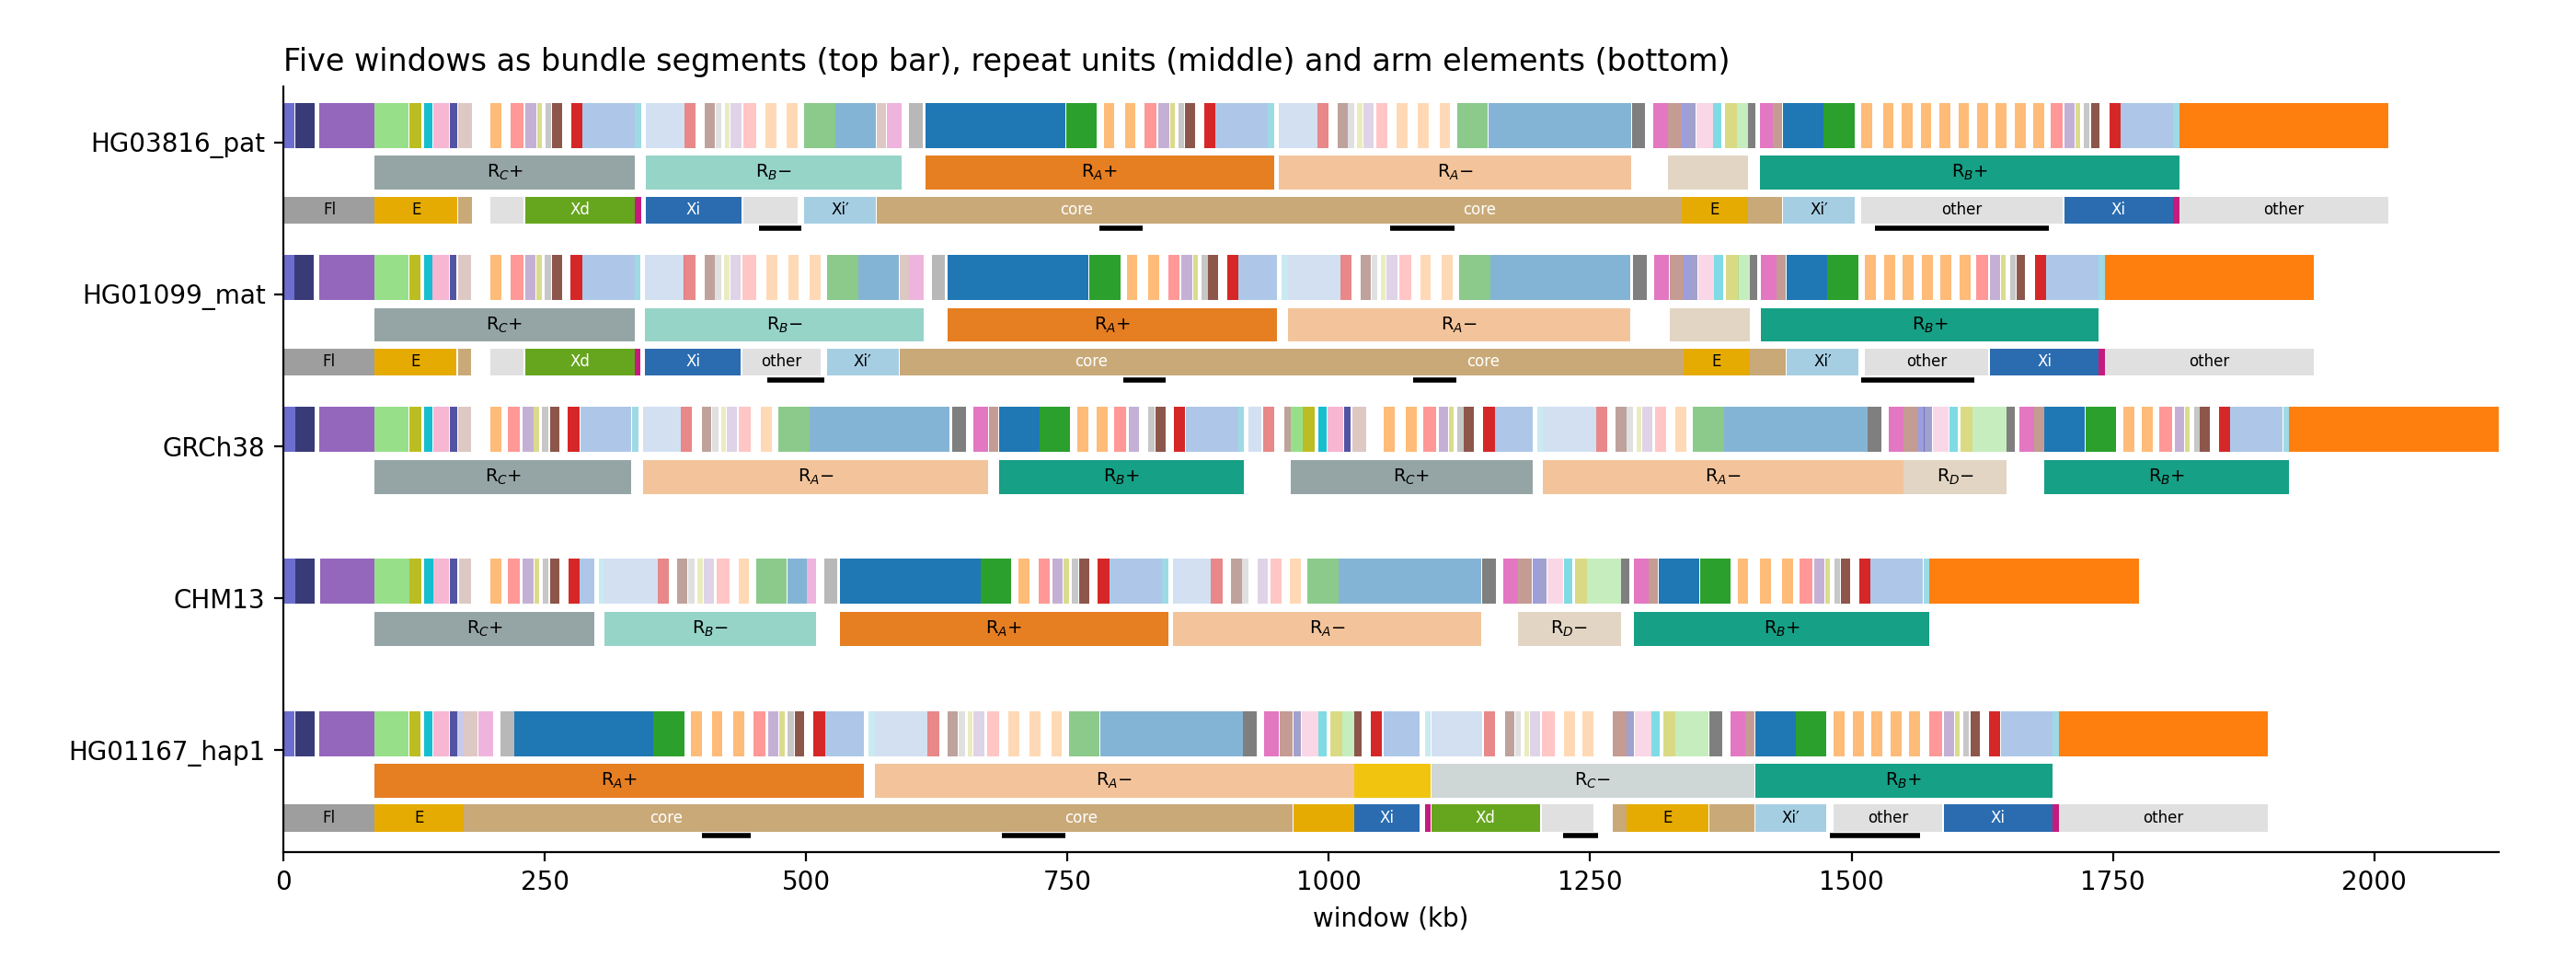
\includegraphics[width=\linewidth]{../figures/window_bundles.png}
\caption{Five SMN windows in the study's bundle decomposition (\texttt{pangea cohort bundle decomp}, $w=48$, $k=55$, $r=4$; all settings in Table~\ref{tab:decomp}): for each
window, bundle segments (top bar; one color per bundle id; pale, reverse
direction), the study's repeat units (middle bar, family colors as in Fig.~\ref{fig:allhaps}) and, for the three windows
with an \RU{A}+ \RU{A}$-$ pair, the arm elements of step 28b (bottom bar, colors as in Fig.~\ref{fig:palindrome}; black lines,
the $\sim$20~kb tandem arrays).}\label{fig:pgraph}
\end{figure}


\begin{table}[htbp]\footnotesize\centering
\caption{Repeat-unit families with ten or more occurrences, from PANGEA's \texttt{repeat-units} output
(\texttt{results/decomp/smn.repeat\_units.tsv}) and the bundle decomposition. Occ.: unit occurrences; windows: windows
(haplotypes and the two references) carrying the family; span of an occurrence; bundles: median number of bundle
segments in an occurrence; strand of the occurrence (+/$-$); its relation to the other copy (inverted/direct); core
bundles: the bundle ids present in at least 90\% of the family's occurrences, with the share of the family's bases
they cover (core bp). Bundle ids are those of \texttt{results/decomp/smn.bed}.}\label{tab:unitfam}
\begin{tabular}{@{}lrrlrrrp{4.1cm}r@{}}\toprule
Family & Occ. & Windows & Span, kb (range) & Bundles & +/$-$ & Inv./dir. & Core bundles (number: ids) & Core bp\\\midrule
\tabUnitFam
\bottomrule\end{tabular}
\end{table}

\begin{table}[htbp]\footnotesize\centering
\caption{What each repeat-unit family is made of, in the arm elements of Section~\ref{sec:palindrome}. For every unit
occurrence on the \elHaps{} haplotypes with the head-to-head \RU{A} pair, the share of its bases in each element (core: within the
arm's core; core end; Xi, both parts, Xi$'$ and Xi; S; Xd; E; flank; other: bases in none of these elements), averaged per family, so each row adds to 1; last column, the commonest combination of elements
with a share of at least 0.1, and how many occurrences have it. Families with ten or more such occurrences. Written by
\texttt{40\_numbers.py} from \texttt{results/sv/unit\_family\_elements.tsv} (step 28e).}\label{tab:unitfamel}
\begin{tabular}{@{}lrrrrrrrrrrl@{}}\toprule
Family & Occ. & Hap. & Core & Core end & Xi & S & Xd & E & Flank & Other & Commonest (occ.)\\\midrule
\tabUnitFamEl
\bottomrule\end{tabular}
\end{table}

\textbf{Copy classes.} The study's pipeline names each copy by two paralog-specific bases read in the copy's own
sequence: c.840 in exon~7 and c.*239 in exon~8. An \emph{SMN1} copy carries the SMN1 base at both, an \emph{SMN2}
copy the SMN2 base at both. A \emph{hybrid} carries one of each: \emph{h12} has SMN1's exon~7 and SMN2's exon~8,
\emph{h21} the reverse. A $\Delta$7--8 copy lacks exons 7 and 8. A counted copy lies away from contig ends and gaps and is either whole (all nine exons:
1, 2a, 2b and 3--8) or a $\Delta$7--8 copy (exons 1--6); a \emph{truncated} piece is cut short by a contig end or gap and a \emph{fragment} misses
part of the gene elsewhere, and neither is counted as a copy.

\textbf{Arrangement type.} The \emph{arrangement} of a haplotype is the string of its SMN copies in order along its
window, from the centromeric end to the telomeric end (GRCh38 coordinate order), each written as a class code followed
by its strand. The codes are \texttt{1} (SMN1), \texttt{2} (SMN2), \texttt{h12} and \texttt{h21} (the hybrids),
\texttt{d2} (a $\Delta$7--8 copy of SMN2 type), \texttt{t} (a truncated piece) and \texttt{f} (a fragment). The
strand is \texttt{+} when the copy runs on the forward strand of the window held in GRCh38 orientation (the
orientation read from the window's own sequence), as SMN1 does in GRCh38, and \texttt{-} when it runs on the other.
So ``2-~1+'' is a reversed SMN2 copy on the centromeric side of a forward SMN1 copy, two copies in head-to-head
inverted orientation; ``1+'' is a single forward SMN1 copy; and ``1-~h12+~1+'' is three copies. GRCh38 itself reads
``2+~1+'' and CHM13 ``2-~1+''. ``1-~h21$\pm$'' stands for ``1-~h21+'' and ``1-~h21-'' together.

An
\emph{arrangement type} is one distinct string; haplotypes with the same string share the type. Over the \arrHaps{}
resolved haplotypes (the region on one contig, spanned end to end) there are \arrTypes{} types, \arrOnce{} of them
seen on one haplotype only; the commonest, ``2-~1+'', is on \arrTopN. Uncounted pieces are kept in the strings, which
adds \arrUncTypes{} types (``f-~1-'' and ``t-~2-~1+''), and they are built by the study's pipeline
(\texttt{scripts/05\_haplotype\_calls.py}). \emph{Centromeric} and \emph{telomeric} for a single copy are defined in
Section~\ref{sec:posstrand}.

\textbf{Alignment columns.} The copies are compared through one multiple sequence alignment made by MAFFT: a table
with one row per copy and one \emph{column} per aligned position. A column holds, for each copy, the base it carries
at that position, or a gap (`-') where it has none; MAFFT places the gaps so that the bases in one column are taken
to be the same position of the gene in every copy. The alignment has \nAlnRows{} rows (each copy cut with 2~kb of flank on each
side, all on the SMN1 strand) and \nAlnCols{} columns, more than any one copy's length because an insertion in any
copy adds columns where all other copies have gaps. The \emph{gene-body columns} are those between the flanks,
measured on the GRCh38 SMN1 copy: the \nRefBody{} columns where that copy has a base (its \nRefLen{} bases, less
2{,}000 at each end), plus the \nInsCols{} columns inside that stretch where it has a gap and some other copy has a
base (insertions in other copies, such as longer poly-T runs). That makes \nGeneCols{} gene-body columns. A column is
therefore a position of the alignment, not a base of GRCh38; a position in this document given as chr5:\ldots{} is
the GRCh38 base in that column (for an insertion column, the GRCh38 base just before it).

The \emph{copy distance} is the share of differing bases between two copies (p-distance), counted over the
gene-body columns where both copies carry a base (A, C, G or T); columns where either copy has a gap or an N are
skipped, so a pair is compared over somewhat fewer than \nGeneCols{} columns. \nVarCols{} of the gene-body columns
vary among the copies. The \emph{sequence distance} between two haplotypes is the mean,
taken both ways, of each copy's distance to its nearest copy on the other haplotype. It is computed over all copies,
over SMN1 copies only and over SMN2 copies only; the last two compare lineages without mixing in which genes a
haplotype carries.

\textbf{Copies used.} Of the \nCounted{} counted copies, \nAligned{} were aligned; the \nJoined{} copy the pipeline joined from two
pieces of one contig (an SMN2 copy of HG00597 mat) was not. The \nDelLeftOut{} $\Delta$7--8 copies were then left
out because the aligner misplaced their 6.3-kb deletion, leaving \nCopies{}: \nSMNone{} SMN1, \nSMNtwo{} SMN2,
\nHtwelve{} h12 and \nHtwentyone{} h21. By continental group (1000 Genomes superpopulation of the donor), they are
\spAFR{} AFR, \spEAS{} EAS, \spAMR{} AMR, \spSAS{} SAS and \spEUR{} EUR, \spOther{} from donors with no group in this
scheme (one ASL donor, and HG002 and HG005, which carry no population label in the study's table) and \spNone{} from
GRCh38 and CHM13.

\section{Pipeline steps and software}
Table~\ref{tab:tools} lists each step with the program that does it, its version and what it reads
and writes. The diagrams are drawn by Matplotlib from the distance matrices; PANGEA, MAFFT and IQ-TREE make the
inputs.

\begin{table}[!h]\small\centering
\caption{The steps, in order. \texttt{scripts/run\_all.sh} runs them in order from the project's root.}
\label{tab:tools}
\begin{tabular}{@{}>{\raggedright}p{2.6cm}>{\raggedright}p{3.4cm}>{\raggedright\arraybackslash}p{9.6cm}@{}}
\toprule
Step & Tool (version) & What it does here \\
\midrule
Bundle decomposition & PANGEA \verPangea{}, \texttt{cohort bundle decomp}, \texttt{repeat-units}~\cite{chin2023} & \texttt{00\_windows\_decomp.py}: extracts the \wfN{} windows, decomposes them together (settings in Table~\ref{tab:decomp}) and calls the repeat units; writes \texttt{results/decomp/}. \\
Structural distance & PANGEA \verPangea{}, \texttt{cohort bundle dist}~\cite{chin2023} & Reads the study's bundle
decomposition of every window (\texttt{results/decomp/smn.bed}) and scores each pair of windows by its top bundles;
writes \texttt{results/sv/smn\_struct.dist}. Step 01b does the same on the finer decomposition (\texttt{results/bundles/smn.bed}; Section~\ref{sec:fine}). \\
Copy alignment & MAFFT \verMafft{}, FFT-NS-2~\cite{katoh2013} & \texttt{02\_copy\_alignment.sh}: aligns the \nAligned{} copies
(gene body with flanks, all on the SMN1 strand) progressively; writes \texttt{results/sv/copies.aln.fa}. Its engine,
\texttt{disttbfast}, takes most of the run time. \\
ML tree & IQ-TREE \verIqtree{}, \iqModel, \iqBoot{} ultrafast bootstraps~\cite{minh2020,hoang2018} & \texttt{04a\_ml\_tree.sh}: the
\iqSeqs{} rows (the copies without the $\Delta$7--8 copies, plus four apes) over the \iqCols{} gene-body columns, rooted
on the orangutan copy (\iqIdent{} identical sequences set aside and re-attached); \texttt{29\_ml\_tree\_clades.py} reports
its clades; Fig.~\ref{fig:mltree}. \\
Distances, tests, trees, plots & Python: NumPy \verNumpy{}~\cite{harris2020}, pandas \verPandas{}, SciPy \verScipy{}~\cite{virtanen2020},
Matplotlib \verMpl{}~\cite{matplotlib} & \texttt{07\_compare.py}: p-distances over the gene-body columns; Mantel tests
(Spearman, \nPerm{} permutations)~\cite{mantel1967}; the UPGMA structure tree with optimal leaf order; cophenetic correlation;
nearest-neighbor agreement; the three figures. \\
Ape bases at the history sites & agc-rs, Python (as above) & \texttt{13c\_ape\_site\_reads.py}: each ape's base at every S and A/B site, read from its raw primary-assembly sequence by local alignment of the GRCh38 context (\rdAcc{} of \rdN{} reads kept); step~16 uses these bases. \texttt{36\_window\_flanks.py}: how each SMN window was taken and its single-copy ends. \\
Spacer sequence & Python: edlib \verEdlib{}& \texttt{28c\_spacer\_sequence.py}: puts each S occurrence in the reference orientation by \sK-mer containment and aligns it end to end to the others (global edit distance), which gives the Sa and St variants of Section~\ref{sec:palindrome}. \\
This document's numbers & Python (as above) & \texttt{40\_numbers.py}: every number below as a macro, with checks;
recomputes the copy tree to place the \cpe{} copies. \\
\bottomrule
\end{tabular}
\end{table}

\section{Large-scale structure against SMN sequence}\label{sec:structseq}
\subsection{Haplotypes with similar structure carry similar SMN copies (Fig.~\ref{fig:scatter})}\label{sec:cophen}
Each dot is one pair of haplotypes. Pairs of the same arrangement type (Section~\ref{sec:compared}) are drawn in orange, pairs of different types in gray. Same-type pairs sit low and left:
their median structural distance is \structSame{} against \structDiff{} for different-type pairs, and their median
sequence distance (all copies) \seqSame{} against \seqDiff{} differences per kb. The horizontal bands come from
the sequence distance being a small whole number of differences divided by the gene length.
The rank correlation, tested by the Mantel test (the haplotype labels of one distance matrix shuffled, \nPerm{} times),
is \mantelAll{} for all copies and \mOneR{} for SMN1 copies; each $p$ is \mantelP{}, the smallest \nPerm{} shuffles
can give, also when shuffling only within African-ancestry and other haplotypes, or within each of five continental groups (\textbf{Shuffles within five groups}, below). Within African-ancestry haplotypes the
SMN1 correlation is \mOneAFRlower{} (\mOneAFRR{}, \mOneAFRN{} haplotypes) than within the rest (\mOneNonAFRR{},
\mOneNonAFRN{} haplotypes).

\begin{figure}[h]\centering
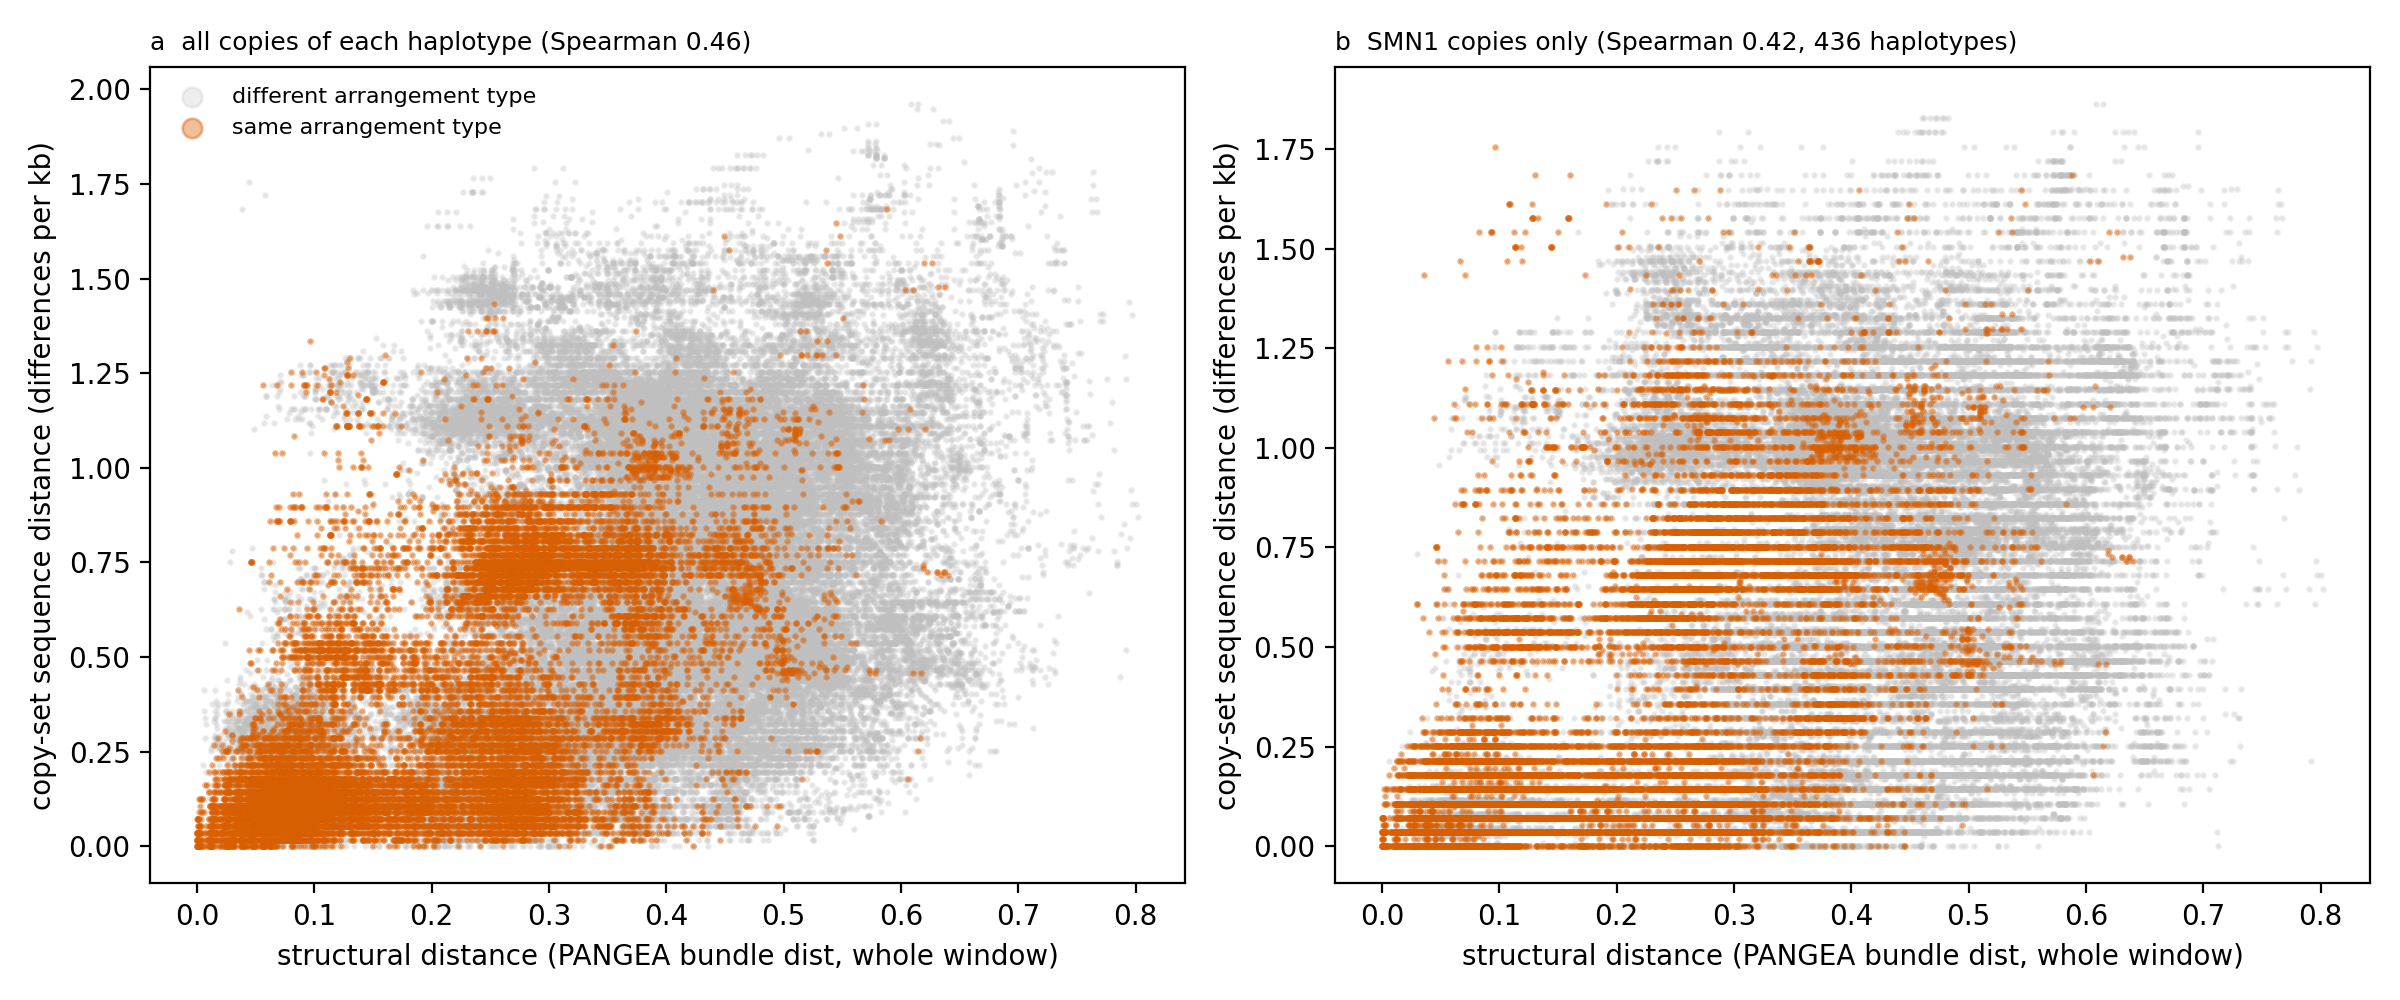
\includegraphics[width=\linewidth]{../figures/hap_scatter.png}
\caption{Each pair of haplotypes by structural distance (x; PANGEA bundle distance over the whole window) and
sequence distance of their SMN copies (y; differences per kb). \textbf{a}, all copies; \textbf{b}, SMN1 copies only.
Orange, the two haplotypes have the same arrangement type. Drawn by \texttt{07\_compare.py}.}
\label{fig:scatter}
\end{figure}

\paragraph{Within one arrangement type (Fig.~\ref{fig:scattype}).} Drawn one type at a time, the same-type pairs of
the \stTypes{} types carried by ten or more haplotypes (\stTypeHaps{} haplotypes) do not form one cloud each: most
types split into a few clusters of pairs, low on both axes or higher on both. Across those clusters, structure and
sequence still go together inside a type: the within-type rank correlation is \stRlo{} to \stRhi{} in \stSigTypes{}
types (\stRbig{} for ``2-~1+''; Mantel test, haplotype labels shuffled within the type, each $p$ at the floor
\mantelP{}). The exception is \stNsType{} (\stNsN{} haplotypes, \stNsR{}, $p = \stNsP{}$). By eye, within a single
cluster of pairs the correlation is weak, so much of the within-type correlation comes from the clusters sitting apart;
this was not tested.

Types differ in how varied they are (Fig.~\ref{fig:scattype}h). The single-copy types are the most varied in
sequence: median distance \stQOne{} differences per kb for ``1-'' and \stQPlus{} for ``1+'', against \stQBig{} for
``2-~1+'' and \stQMix{} for ``1-~2+''. ``1-'' is also the most varied in structure (median \stSOne{}, against
\stSMix{} for ``1-~2+'' and \stSBig{} for ``2-~1+'').

\paragraph{Structural distance follows window length.} PANGEA's bundle distance scores the whole window, so two
haplotypes whose windows differ in length differ in structure even with the same SMN arrangement. Over same-type pairs
the structural distance has a rank correlation of \stLenSame{} with the difference in window length
(Fig.~\ref{fig:scattype}i; \stLenAll{} over all pairs), while the sequence distance has \stLenSeqAll{} over all pairs.
The single-copy windows are also the shortest (median \stLOne{} kb for ``1-'', \stLPlus{} kb for ``1+'', against
\stLBig{} kb for ``2-~1+''). Holding the length difference fixed (partial rank correlation), structure and sequence still
go together in the common two-copy types (\stPBig{} for ``2-~1+'', \stPInv{} for ``1-~1+'', \stPFlip{} for ``2-~1-''),
less in ``1+'' (\stPPlus{}), and hardly at all in ``1-'' (\stPOne{}) and ``1-~2+'' (\stPMix{}). So in those two types
the structural spread is mostly a matter of length, not of what the copies carry. Window length here is the length of
the copy-bearing window; every haplotype tested has one.

\begin{figure}[p]\centering
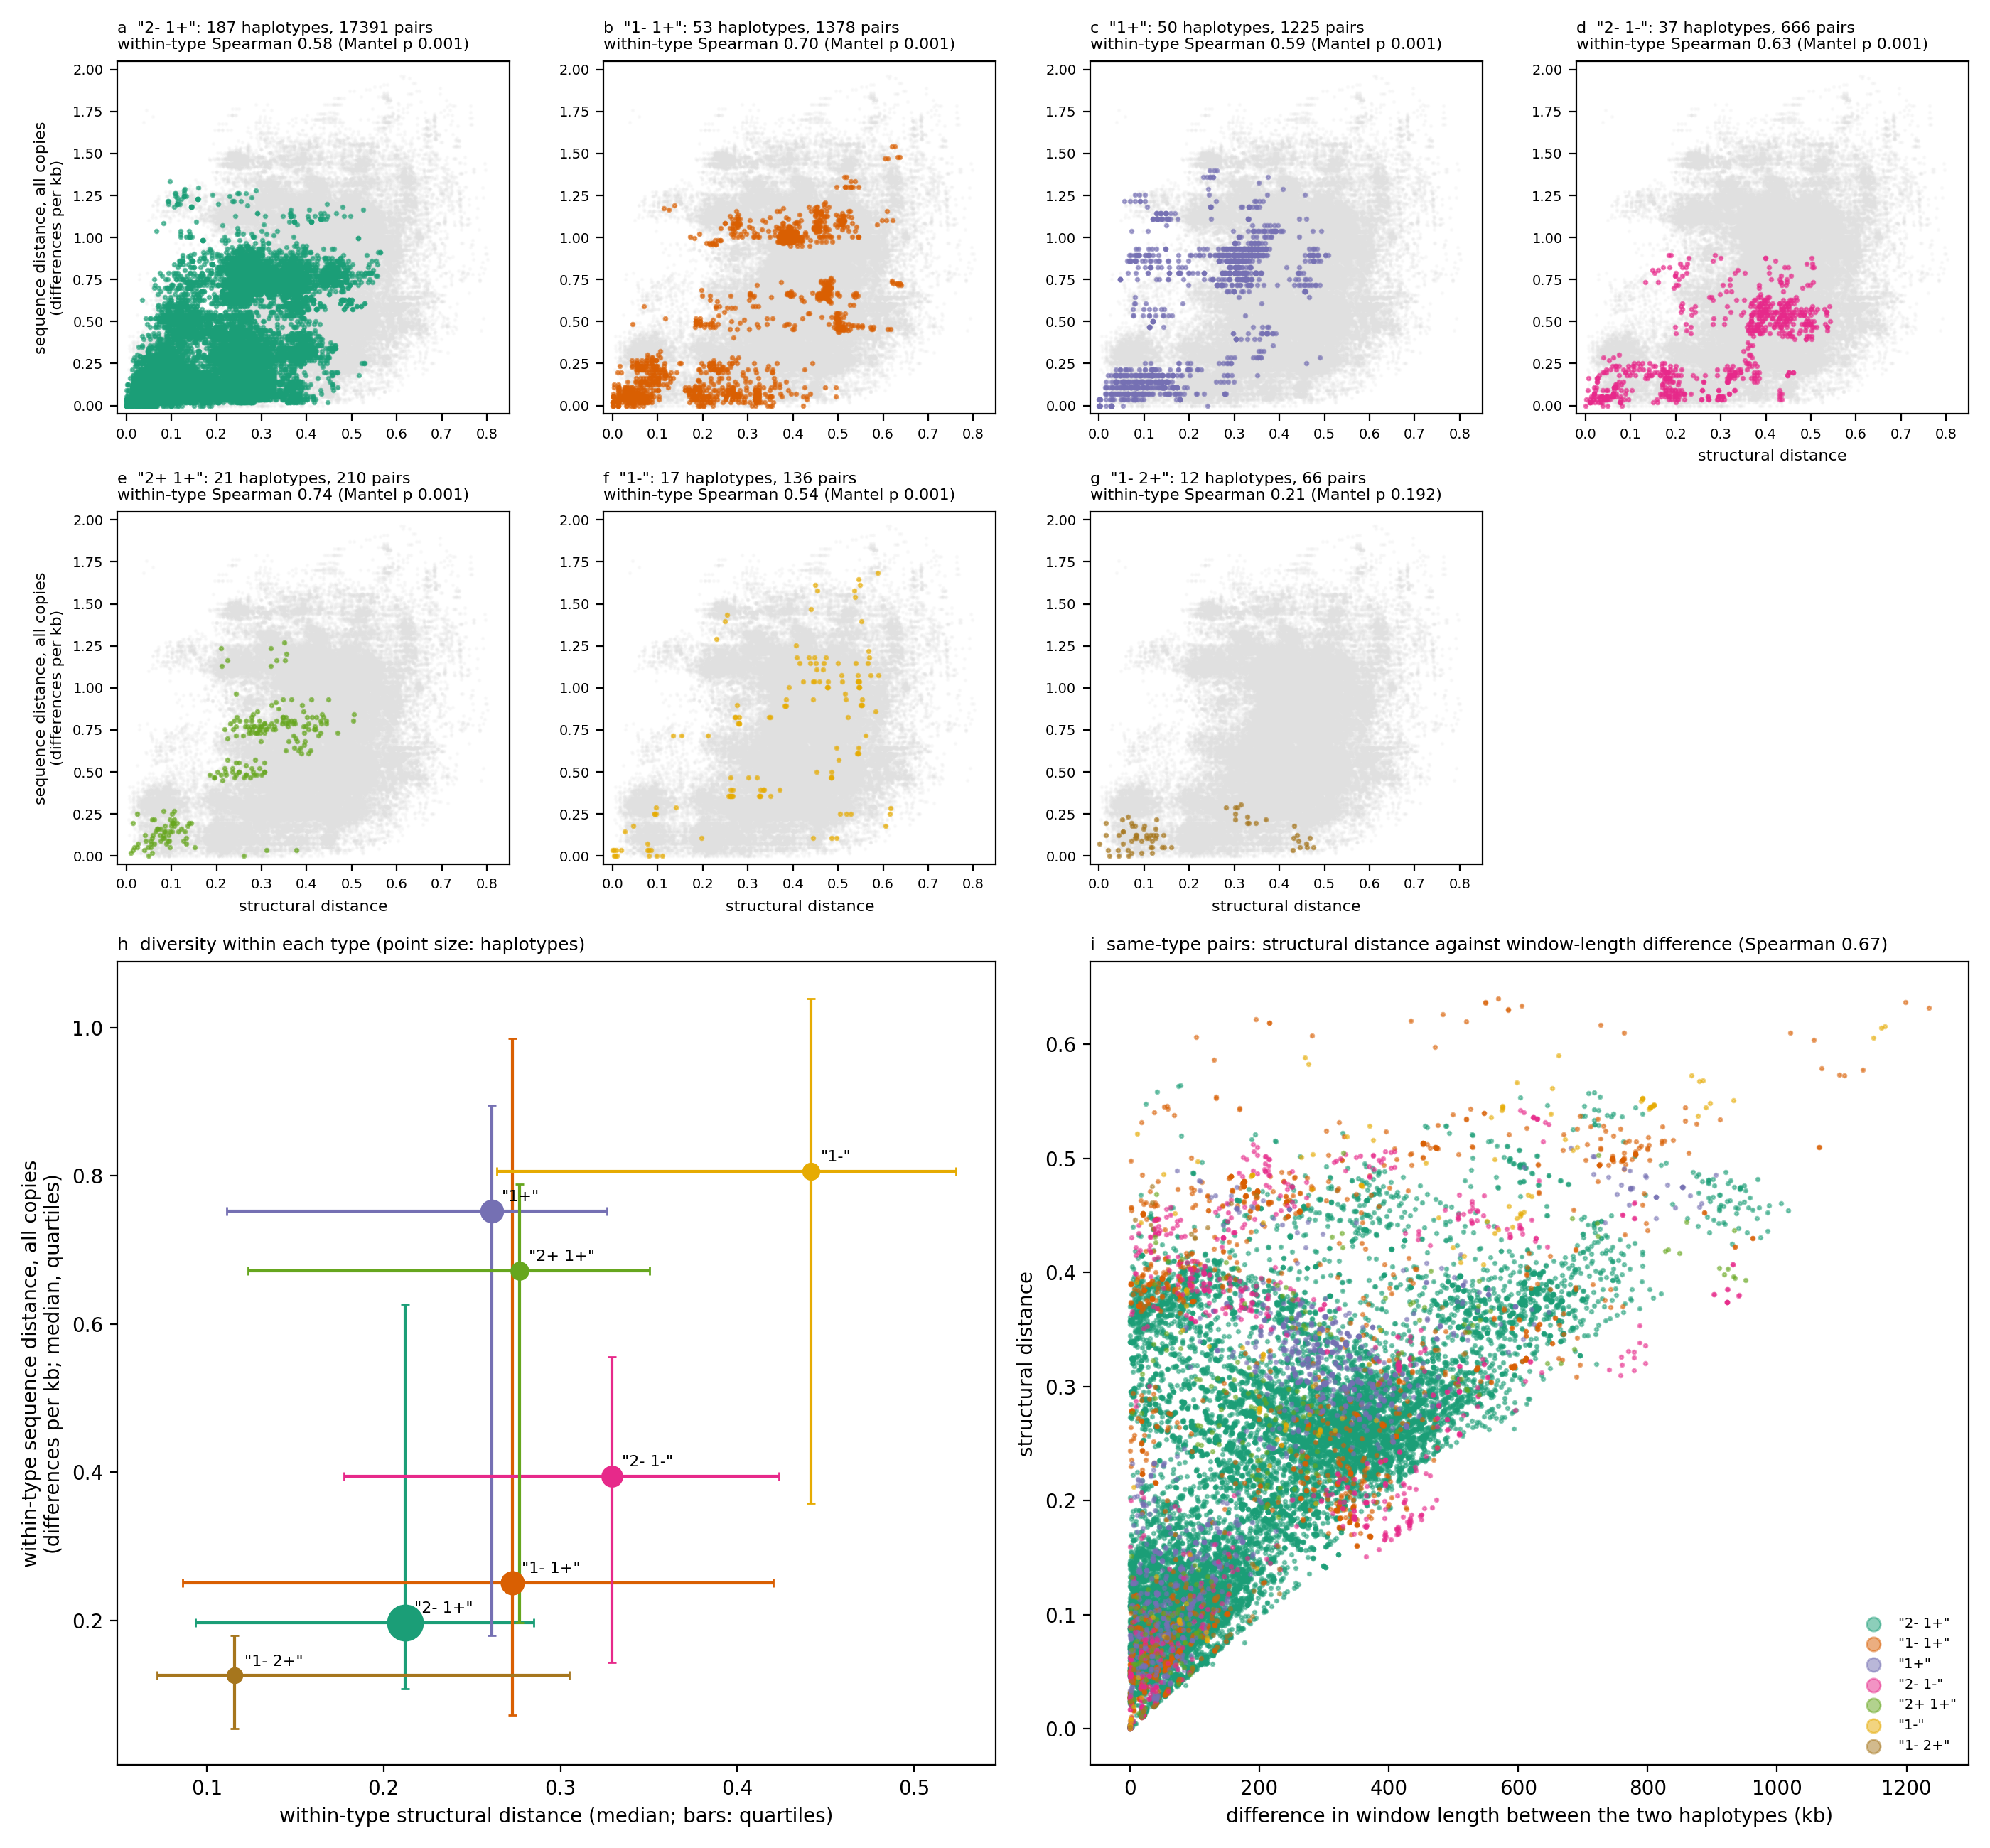
\includegraphics[width=\linewidth]{../figures/hap_scatter_bytype.png}
\caption{Fig.~\ref{fig:scatter}a taken apart by arrangement type. \textbf{a--g}, pairs of the same type (colored)
over all other pairs (gray), one panel per type with ten or more haplotypes, with the within-type rank correlation and
its Mantel $p$. \textbf{h}, within-type median structural and sequence distance; bars, quartiles; point size, number of
haplotypes. \textbf{i}, same-type pairs: structural distance against the difference in window length. Drawn by
\texttt{24\_scatter\_by\_type.py}.}
\label{fig:scattype}
\end{figure}

\paragraph{The two trees agree only loosely.} The structure tree of the \nTangle{} haplotypes that carry an SMN1 copy
(the \nHapsResSMNone{} resolved donor haplotypes with one, plus GRCh38 and CHM13; UPGMA on structural distance) and the
gene-body maximum-likelihood tree (main text, Fig.~\ref{fig:mltree}) agree only loosely: the cophenetic correlation, the
correlation between the heights at which two haplotypes join in the structure tree and the distance between their SMN1
copies along the branches of the maximum-likelihood tree (for a haplotype with two SMN1 copies, each copy's nearest copy
in the other haplotype, averaged both ways), is \cophenetic{}. These tree distances follow the p-distances closely
(Spearman \cophMlVsP). Where the trees do agree is taken up below, by SMN1 lineage make-up (Section~\ref{sec:lintrees}) and
as bands (Section~\ref{sec:bands}).

\subsection{A copy's nearest sequence neighbor tends to share its arrangement type (Table~\ref{tab:nn})}
Each of the \nCopies{} copies is given labels of its context in the haplotype: its copy order, its rank among all SMN copies of the
window, SMN2 and hybrids included (centromeric, middle, telomeric or the only one; defined in
Section~\ref{sec:posstrand}), its strand on GRCh38, the form of the NAIP gene at its 3$'$ side, the downstream
environment, the arrangement type of its haplotype and the donor's continental group (copies on unresolved haplotypes
are not assessed). The main text's Fig.~\ref{fig:mltree} draws the class, haplogroup, arm (cenSMN, telSMN or no \RU{A} pair), arrangement type and continental group
of each copy along the maximum-likelihood tree.

For each copy, the nearest copy by sequence on another haplotype was found
within SMN1 and within SMN2 separately, and the share of copies whose neighbor has the same label was compared with
the share expected by chance, from \nPerm{} shuffles of the label (Table~\ref{tab:nn}). For SMN1, neighbors share the
arrangement type \agArrOne{} of the time against \agArrNullOne{} by chance within ancestry groups, copy order
\agPosOne{} against \agPosNullOne{}, and strand \agStrOne{} against \agStrNullOne{}. For SMN2 the same figures are
\agArrTwo{} against \agArrNullTwo{}, \agPosTwo{} against \agPosNullTwo{}, and \agStrTwo{} against \agStrNullTwo{}.
Of the labels tested within ancestry groups, the arrangement type rises most above chance in both genes; ancestry itself, which can only be shuffled among all copies, rises by about as much in SMN1 (Table~\ref{tab:nn}). Nearly every SMN2 copy sits in an SMN2-type
environment, so that label adds little there (\agEnvTwo{} against \agEnvNullTwo{}, $p=\agEnvPTwo$).

\begin{table}[h]\small\centering
\caption{Nearest sequence neighbor on another haplotype: share with the same label. $n$, copies with the label
assessed; obs., observed share; chance, mean over \nPerm{} shuffles of the label among all copies, and among
copies of the same ancestry group (African ancestry or not); $p$ for the latter. Ancestry itself is tested only
against all-copy shuffles. Written by \texttt{40\_numbers.py} from \texttt{results/sv/copy\_neighbor\_agreement.tsv}.}
\label{tab:nn}
\setlength{\tabcolsep}{3.5pt}
\begin{tabular}{@{}>{\raggedright}p{4.3cm}rrrrr rrrrr@{}}
\toprule
& \multicolumn{5}{c}{SMN1 copies} & \multicolumn{5}{c}{SMN2 copies}\\
\cmidrule(lr){2-6}\cmidrule(l){7-11}
Label & $n$ & obs. & chance & \shortstack{chance\\ in group} & \shortstack{$p$\\ in group} & $n$ & obs. & chance & \shortstack{chance\\ in group} & \shortstack{$p$\\ in group} \\
\midrule
\tabNeighbor
\bottomrule
\end{tabular}
\end{table}


\subsection{Haplotypes with two B copies cluster in both trees; those with one B have like neighbors in both but cluster tightly only by sequence}\label{sec:lintrees}
Do haplotypes with the same SMN1 lineage make-up (Table~\ref{tab:lincomp}) sit together in the structure tree and in
the SMN1 sequence tree? \texttt{19c\_lineage\_in\_both\_trees.py} takes, for the same \tmHaps{} haplotypes,
the structure tree (UPGMA with optimal leaf order on bundle distance) and the gene-body maximum-likelihood tree
(Fig.~\ref{fig:mltree}), read at the haplotype level: the distance between two haplotypes is the tree distance
between their SMN1 copies, each copy to its nearest copy on the other haplotype, both ways, averaged, and a haplotype's
leaf is its first SMN1 copy in the tree's leaf order. It asks, for each
make-up, how often a haplotype's nearest neighbor in the tree has the same make-up, against labels shuffled across all
haplotypes and shuffled only within AFR and within non-AFR (\tmPerm{} shuffles each, so $p$ stops at \tmPmin), and
into how many separate runs of leaves the group falls.
\begin{itemize}
\item \textbf{Two B copies} (\tmBBn{} haplotypes, \tmBBafr{} AFR; mostly one B1 with one B2): the nearest neighbor
shares the make-up in \tmBBnnStruct{} of cases in the structure tree and \tmBBnnSeq{} in the sequence tree (chance
\tmBBchanceStruct, or \tmBBchanceAfrStruct{} within AFR; $p=\tmBBpStruct$ and $\tmBBpSeq$ whichever way labels are
shuffled). They form \tmBBrunsStruct{} runs of leaves in the structure tree and \tmBBrunsSeq{} in the sequence tree;
their median tree distance in the structure tree is \tmBBmedStruct, against \tmMedAll{} over all pairs. Taking the 16 structure
clusters and the sequence clusters of Section~\ref{sec:bands} (supported clades of the maximum-likelihood tree), \tmBBkStruct{} fall in one structure cluster (of \tmBBkStructSize{} haplotypes), \tmBBkSeq{} in
one sequence cluster (of \tmBBkSeqSize), and \tmBBkBoth{} in both.
\item \textbf{One B only} (\tmBn, \tmBafr{} AFR): in both trees a haplotype's nearest neighbor shares the make-up
more often than by chance (structure \tmBnnStruct, sequence \tmBnnSeq, against \tmBchanceStruct; $p=\tmBpStruct$ in each,
also within AFR), so they sit in small groups in both. But only in the sequence tree do these groups gather: \tmBrunsSeq{}
runs of leaves there, \tmBrunsStruct{} in the structure tree, where their median tree distance (\tmBmedStruct) is above
the \tmMedAll{} of all pairs. At 16 clusters \tmBkSeq{} share a sequence cluster but only
\tmBkBoth{} share a cluster in both trees: B as a sequence lineage turns up in several arrangements.
\item \textbf{Two A} (\tmAAn; Table~\ref{tab:lincomp} counts \ldCompAA, the extra one an unresolved haplotype, which is in
no tree) group in the sequence tree ($p=\tmAApSeq$) and not in the structure tree
($p=\tmAApStruct$). The \tmABn{} haplotypes with one A and one B copy are too few to test.
\end{itemize}
The shuffles treat haplotypes as independent, the structure tree has no support values, and many structural
distances are exactly \tmMedAll, which makes the median test coarse.


\subsection{Bands of arrangement and haplogroup link the two trees at every clade setting; the cenSMN arm type splits the two large structure clusters (Fig.~\ref{fig:tangclus})}\label{sec:bands}
The lineage make-up explains one group of haplotypes that sit together in both trees (Section~\ref{sec:lintrees}). To find others without choosing them by
eye, \texttt{19b\_ml\_bands.py} cuts the structure tree into \setK{} clusters (UPGMA, as above) and groups the SMN1
copies by the gene-body maximum-likelihood tree: each copy goes to the smallest clade with ultrafast-bootstrap support
$\ge$\setMLsup{} holding at least \setMLmin{} SMN1 copies of these haplotypes, or to the rest of the human clade. This
gives \mlbClusters{} sequence clusters (\path{results/sv/ml_seq_clusters.tsv}): S1-3 (support \mlbThreeSup), S1-2
(\mlbTwoSup), S1-8 (\mlbEightSup, the B2 copies), S1-9 (\mlbNineSup) inside S1-6 (\mlbSixSup; this clade is lineage B1, holding \hgBoneSix{} of the \hgSixB{} S1-6 copies),
three small clades of S1-4 and S1-5 copies, and the rest (\mlbRestCopies{} copies, mostly S1-1 and S1-10). A haplotype
with two SMN1 copies takes the combined label, \mlbLabels{} labels in all. Every structure-cluster by label pair is
tested for more shared haplotypes than chance when it holds five or more haplotypes (hypergeometric, Bonferroni
over all such pairs). Three pairs share at least \mlbMinOv{} haplotypes at $p<10^{-\mlbAlphaExp}$; leaf
positions run from 0 at the bottom of a tree to 1 at the top of Fig.~\ref{fig:tangclus} (for the sequence tree, the
median over the band's SMN1 copies).
\begin{itemize}
\item \textbf{The bulk} (red): \cbBulkn{} haplotypes against \cbBulkexp{} expected ($p=\cbBulkp$), mostly ``2-~1+''
(\cbBulktopArr), from every group, whose SMN1 copy lies outside the supported clades. Significant but loose: it is
the middle of the structure tree and the unresolved part of the sequence tree.
\item \textbf{An S1-2 band} (blue): \cbTwon{} haplotypes against \cbTwoexp{} expected ($p=\cbTwop$), at the top of
the structure tree (\cbTwoposS) and in the lower part of the sequence tree (\cbTwoposG). \cbTwohg{} carry an SMN1 copy
assigned to Chen et al.'s S1-2 or S1-2c~\cite{chen2023}; \cbTwotopArr{} are ``2-~1-''. Each has one SMN1 copy, and all
\cbTworev{} are reversed against GRCh38 (\cbTwotel{} telomeric, \cbTwosingle{} alone on the haplotype). None is from an
AFR donor.
\item \textbf{The B1\,+\,B2 band} (purple) of Section~\ref{sec:lintrees}: \cbABn{} haplotypes against \cbABexp{} expected
($p=\cbABp$), all ``1-~1+'', \cbABafr{} of them AFR; B1 is at cenSMN and B2 at telSMN on \cbABcen{} of them. Of the \linMixHaps{} haplotypes that carry B1 and B2, the one outside the band, \cbABoutNames, has the same B1-at-cenSMN layout and lies in structure cluster \cbABoutClu, so the \linMixBoneCenRev{} such haplotypes of Section~\ref{sec:posstrand} are these \cbABcen{} plus it.
\end{itemize}
One other pair, of \mlbSmallOv{} haplotypes, reaches only $p=$\,\mlbSmallP. The \cbSThreeN{} haplotypes labeled S1-3
form no band at this scale: \cbSThreeBulk{} fall in the bulk's structure cluster and \cbSThreeAB{} in the B1\,+\,B2
band's, neither more than chance (corrected $p=1$). There are \mlThreeN{} S1-3 copies, one per haplotype; over all of them the S1-3 clade has support \mlThreeSup{} and holds no other copy. Two more of Chen et al.'s haplogroups are likewise clades holding only their own copies: S1-8 (\mlEightCladeN{} copies, support \mlEightCladeSup) and the S1-9 family (S1-9, S1-9c and S1-9d; \mlNineFamN{} copies, support \mlNineFamSup; \path{results/sv/mltree_clades.tsv}). One (HG00280
hap1) lies on a haplotype without a structural distance and so is not in Fig.~\ref{fig:tangclus}; among the other
\mlbThreeTree{} the S1-3 clade has support \mlbThreeSup. Of those \mlbThreeTree{} haplotypes, \mlbThreeOnly{} carry only S1-3,
and \mlbThreePlus{} also carries a copy outside the supported clades. With the finer bundles the S1-3 haplotypes form a band (Section~\ref{sec:fine}).

\paragraph{The bands against arm form.} \texttt{28e\_families\_bands.py} sets the bands and the structure clusters beside
the arm types of Section~\ref{sec:palindrome} (\path{results/sv/armform_struct.tsv}, \path{results/sv/armform_bands.tsv}).
Among the haplotypes with the head-to-head \RU{A} pair, the bulk band's structure cluster (\afBulkClu{} haplotypes) holds
\afBulkPair, every one with a C1 cenSMN arm (\afBulkCZero{} C0), and the B1\,+\,B2 band's cluster (\afMixClu{}
haplotypes) holds \afMixPair, \afMixCZero{} of them C0 and \afMixCOne{} C1 (Fisher $p=$\,\afPC). The telSMN arm type is
mixed in both: T1 on \afBulkTOne{} of the \afBulkPair{} against \afMixTOne{} of the \afMixPair{} ($p=$\,\afP). The
B1\,+\,B2 band's \cbABn{} haplotypes are all C0 (\afABCZTOne{} C0|T1, \afABCZTZero{} C0|T0); the bulk band's
\afBulkBandPair{} with the pair are all C1 (\afBulkCOTZ{} C1|T0, \afBulkCOTO{} C1|T1), and \afBulkNoPair{} have no pair;
the S1-2 band has none with the pair. Of the repeat-unit families, the one that best separates T1 from T0 haplotypes is
family~\RU{\afSigFam}, mostly Xi$'$ and Xi (Table~\ref{tab:unitfamel}), on \afSigTOne{} of the \afTOneAll{} T1 haplotypes against
\afSigTZero{} of the \afTZeroAll{} T0. It is also on \afSigNoPair{} of its \afSigHaps{} haplotypes without the pair. Their arms cannot be typed from an axis, so \texttt{28h\_g\_unpaired.py}
reads every S from its nearest SMN copy outward, by bundle id only, and calls an S site T1-like when E lies between the
copy and S and Xi's bundles lie on both sides of S (\path{results/sv/g_unpaired.json}). On the pair
haplotypes this finds a T1-like site on \gValTOne{} of \gValTOneN{} T1 haplotypes and \gValTZero{} of \gValTZeroN{} T0. Of the
\gUnpG{} family-\afSigFam{} haplotypes without the pair \gUnpGTOne{} have one, against \gUnpNoGTOne{} of the \gUnpNoG{} without it; by SMN1
label, all \gSThree{} S1-3 haplotypes among them but only \gSTwo{} of the \gSTwoN{} S1-2 haplotypes. The rule rests on bundle ids and the nearest copy, and was checked only on the pair haplotypes.

\paragraph{The same bands under other settings.} Varying the support
threshold (80, 90, 95) and the clade size (5, 10, 20) gives \mlbSettings{} settings; the same three bands are found at every
one (\path{results/sv/ml_band_sensitivity.tsv}). Haplotypes are treated as
independent, and the structure tree carries no support values.

\paragraph{Shuffles within five groups.} The permutation tests of Section~\ref{sec:lintrees} and
Table~\ref{tab:nn} shuffle labels within AFR and non-AFR only. \texttt{21\_five\_group\_shuffles.py} reruns them with
labels shuffled within each of AFR, AMR, EAS, EUR and SAS (other and references as their own strata). Nothing changes
its conclusion: the Mantel correlations are \fgMantelOne{} (SMN1 copies) and \fgMantelTwo{} (SMN2), $p=\fgMantelPOne$
(the floor); a copy's nearest neighbor shares its arrangement type in \fgArrOne{} of SMN1 copies against \fgArrNullOne{}
by chance and \fgArrTwo{} of SMN2 copies against \fgArrNullTwo{} ($p=\fgArrPOne$); copy order and strand stay above chance
for both genes ($p\le\fgPosPTwo$); the SMN2 environment stays the weakest signal (\fgEnvTwo{} against \fgEnvNullTwo,
$p=\fgEnvPTwo$ with five-group shuffles, against $p=\agEnvPTwo$ with the AFR/non-AFR shuffles of Table~\ref{tab:nn};
the chance levels differ slightly between the two schemes for the same reason). The one-B and two-B make-ups still group in both trees ($p=\fgBBpStruct$, the floor), and two A
still groups in the sequence tree ($p=\fgAApSeq$) and not in the structure tree ($p=\fgAApStruct$). Results are in
\path{results/sv/five_group_shuffles.tsv}.

\begin{figure}[p]\centering
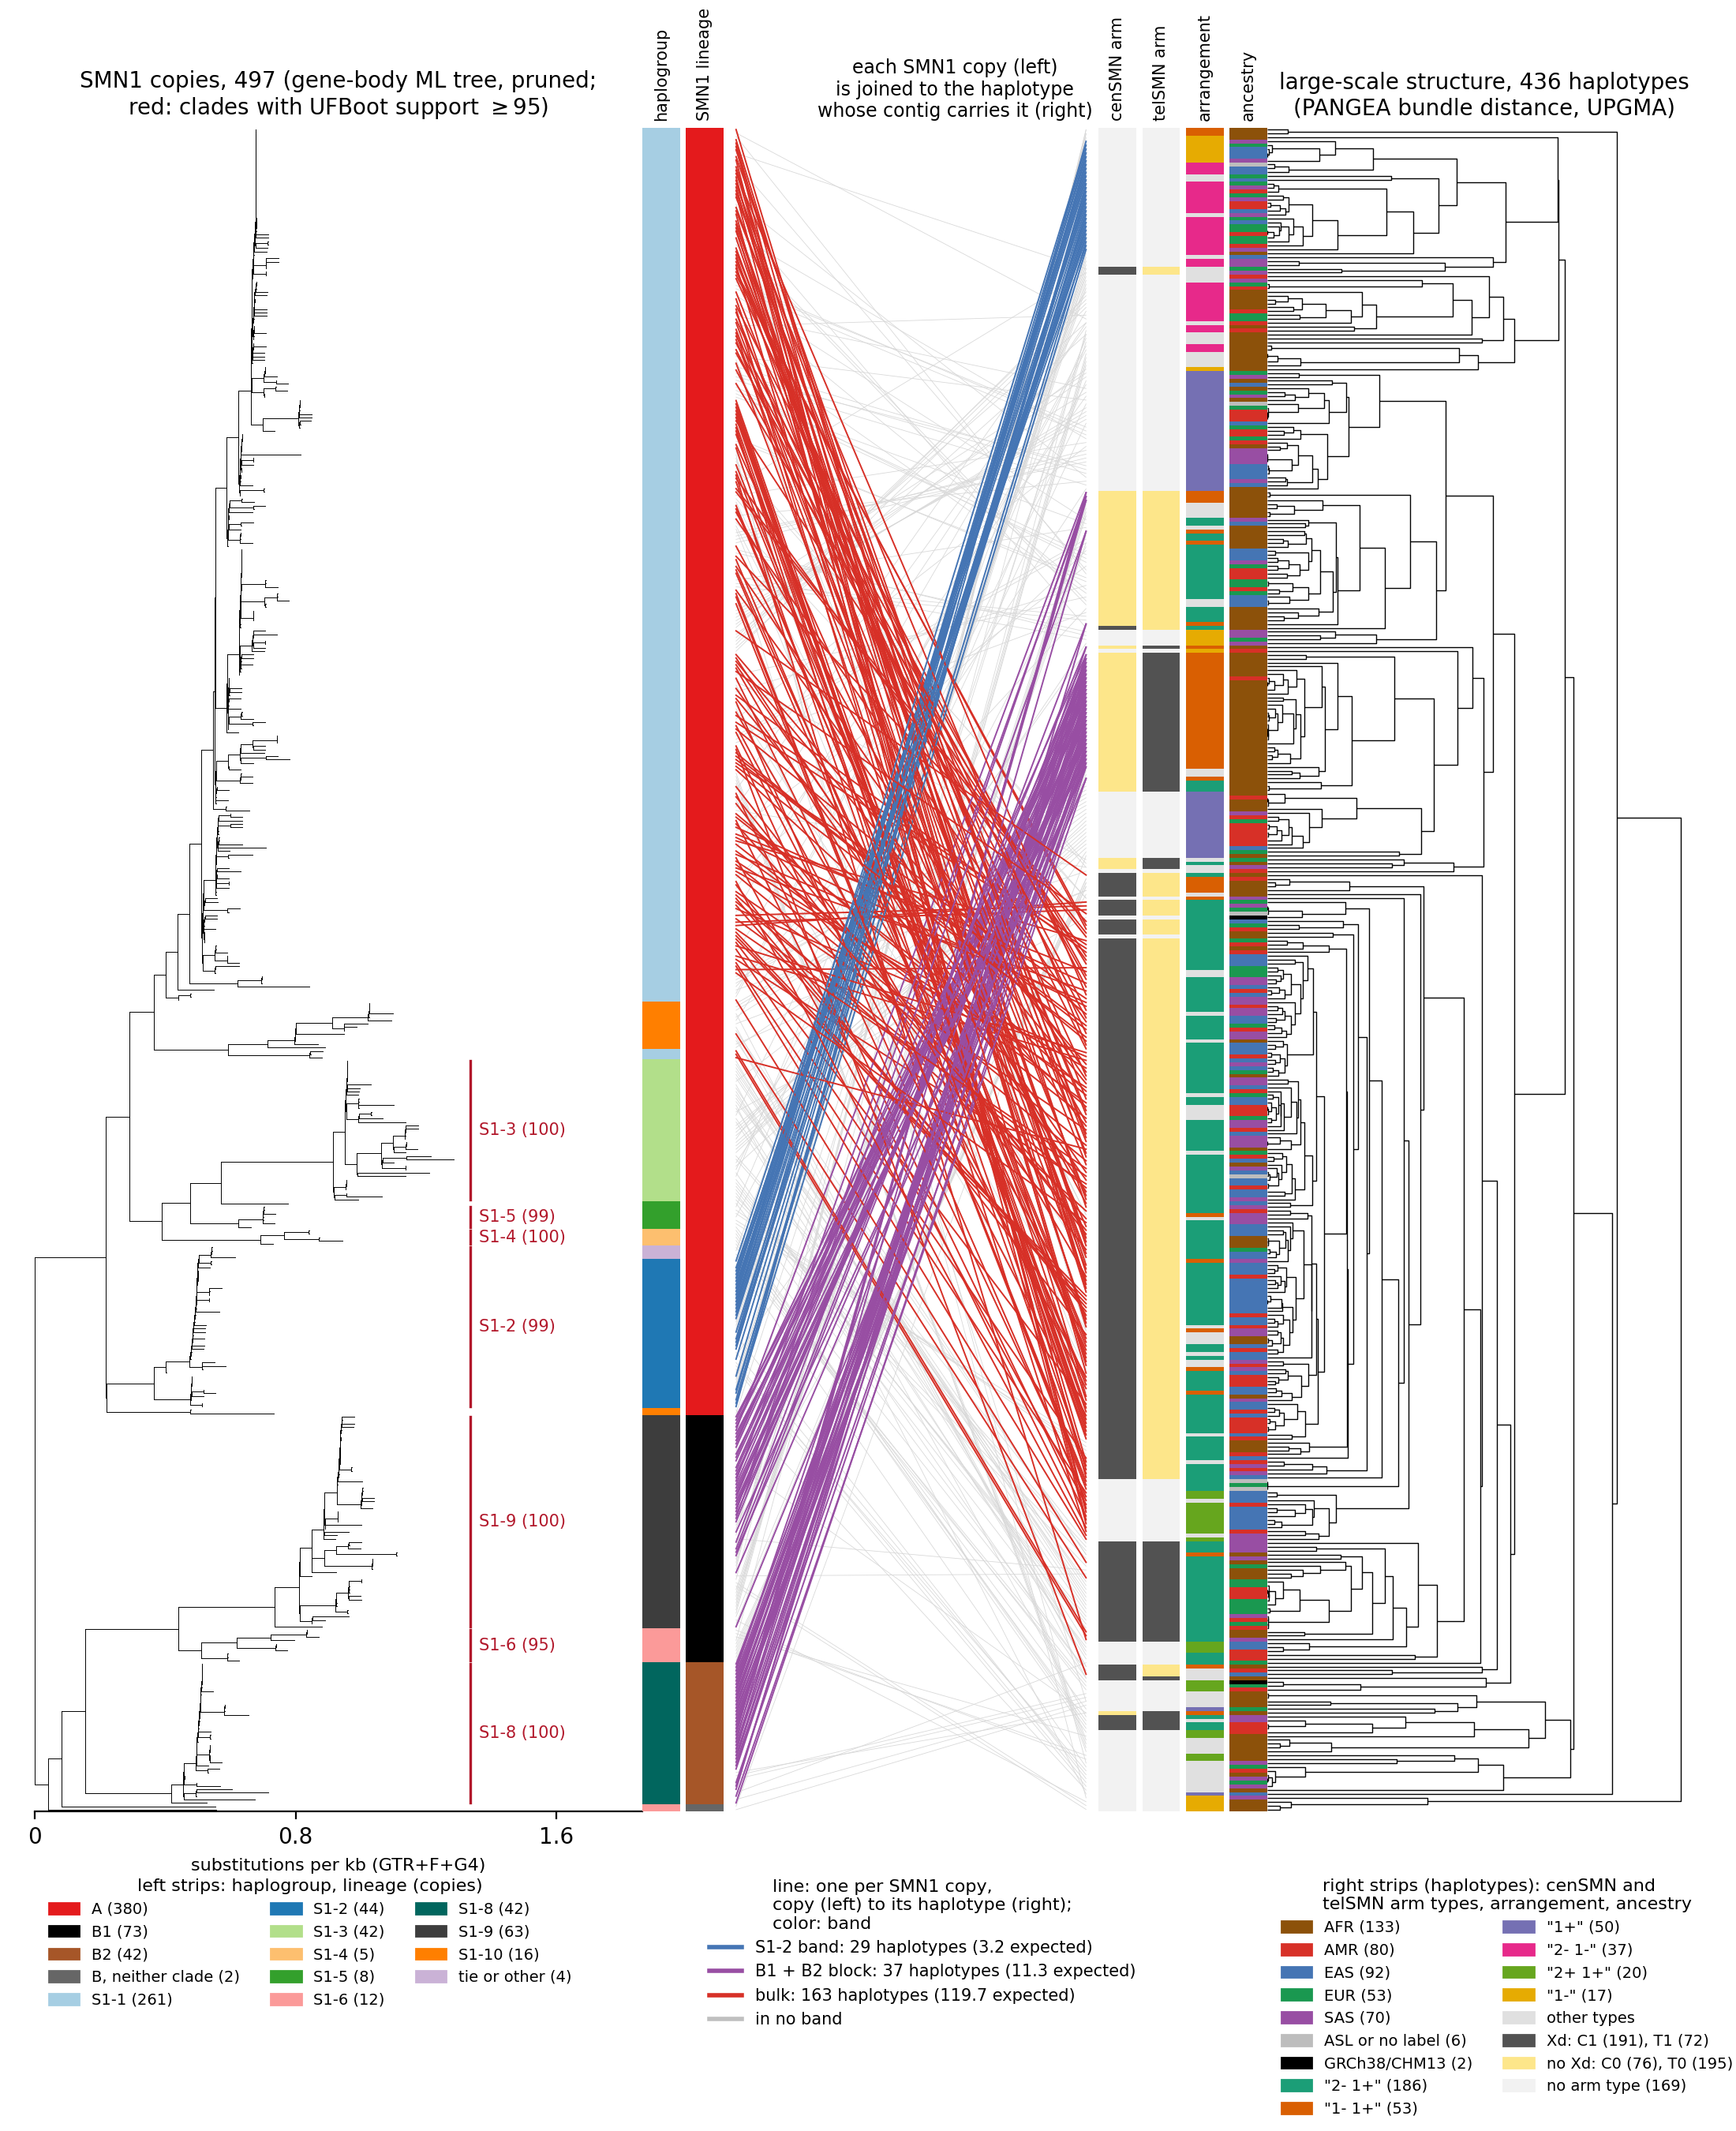
\includegraphics[width=\linewidth,height=0.64\textheight,keepaspectratio]{../figures/tanglegram_ml.png}
\caption{SMN1 sequence against large-scale structure for the \mlbHaps{} haplotypes that carry an SMN1 copy
(\nHapsResSMNone{} resolved haplotypes, GRCh38 and CHM13). The two trees have different leaves: on the left each leaf is
one SMN1 gene copy, on the right each leaf is one haplotype. Left, the gene-body maximum-likelihood tree
(main text, Fig.~\ref{fig:mltree}) pruned to these haplotypes' \mlbCopies{} SMN1 copies (the other \smnOneUnres{} of the tree's \smnOneAll{} SMN1 copies, all lineage A, sit on \smnOneUnresHaps{} unresolved haplotypes, which have no structural distance), leaves facing the middle, with strips for
each copy's Chen et al.\ haplogroup~\cite{chen2023} and lineage. Right, the UPGMA tree on PANGEA's bundle distance
between haplotypes, drawn mirrored so its leaves also face the middle, with strips for each haplotype's cenSMN and telSMN arm
types (Section~\ref{m:arms}; dark gray, the arm carries Xd, C1 or T1; yellow, it does not, C0 or T0; light gray, no arm type, the haplotype not being one of the \palPair{} with the palindrome; the legend counts the \afPairInTree{} pair haplotypes in this tree, the other \afPairOutTree{} carrying no SMN1 copy), arrangement type and continental group. Each SMN1 copy was cut from one haplotype's contig, so it belongs to exactly one haplotype: a line
joins the copy's leaf to the leaf of that haplotype. \mlbOneCopy{} haplotypes carry one SMN1 copy and have one line;
\mlbTwoCopy{} carry two and have two (\mlbOneCopy{} + 2\,$\times$\,\mlbTwoCopy{} = \mlbCopies{} lines). Red bars mark the
clades with ultrafast-bootstrap support (UFBoot, IQ-TREE's bootstrap approximation) $\ge$\setMLsup{} and at least \setMLmin{} SMN1 copies that define the sequence
clusters (support in brackets; supports are over the copies drawn here, so the S1-3 clade, support \mlThreeSup{} over all its \mlThreeN{} copies, shows \mlbThreeSup; the haplogroup legend counts every copy of a haplogroup; the S1-4 and S1-5 clades (support \mlbFourSup{} and \mlbFiveSup) hold only \mlbFourOwn{} and \mlbFiveOwn{} copies outside the smaller clades they contain; a bar spans the copies a clade holds outside smaller such clades, so S1-6's spans the
S1-6 copies outside the S1-9 clade). Lines are colored by band, a structure cluster and a sequence cluster (\setK{} structure clusters) sharing at least
\setMinOverlap{} haplotypes with Bonferroni $p<\setAlpha$: red, the bulk (SMN1 copies outside the supported clades,
mostly S1-1, on ``2-~1+''); blue, the S1-2 band; purple, the ``1-~1+'' haplotypes carrying B1
and B2; gray, no band.}
\label{fig:tangclus}
\end{figure}


\subsection{Inside an arrangement type, haplotypes that share an SMN1 haplogroup are closer in structure as well as in sequence (Fig.~\ref{fig:hgscatter})}\label{sec:hgscatter}
The clusters of pairs inside each arrangement type (Fig.~\ref{fig:scattype}) were tested against Chen et al.'s
haplogroups (Section~\ref{sec:chenhg}; step \texttt{26\_scatter\_lineage\_haplogroup.py}). A haplotype's haplogroup
make-up is the haplogroup families of its SMN1 copies, sorted and joined (for example S1-8+S1-9); the same make-up
implies the same lineage make-up. Of the \hsPairs{} pairs of haplotypes of the same type, \hsSameHg{} share a
haplogroup make-up and \hsSameLin{} a lineage make-up. Pairs that share a haplogroup make-up are closer on both axes:
median sequence distance \hsSeqSame{} against \hsSeqDiff{} differences per kb, and median structural distance
\hsStrSame{} against \hsStrDiff. Type by type, \hsTested{} of the \hsTypes{} types carried by ten or more haplotypes
can be tested (``1-~2+'' has one make-up only). In each, the same-make-up pairs are closer in structure (medians
\hsStrSameLo--\hsStrSameHi{} against \hsStrDiffLo--\hsStrDiffHi) and in sequence (\hsSeqSameLo--\hsSeqSameHi{}
against \hsSeqDiffLo--\hsSeqDiffHi), each at $p=\hsPfloor$, the floor of \hsShuf{} shuffles of the make-up labels
among the type's haplotypes. Kept to pairs of one make-up, the structure--sequence rank correlation inside a type falls
to \hsRhgLo--\hsRhgHi{} (from \hsRallLo--\hsRallHi{} over all pairs of the type) in every tested type but ``1-'',
where it rises (\hsRoneAll{} to \hsRoneHg). So the
clusters inside a type are largely haplogroup clusters, and the haplogroups are what tie structure and sequence
together there; this is the within-type side of the bands of Section~\ref{sec:bands}.

\begin{figure}[p]\centering
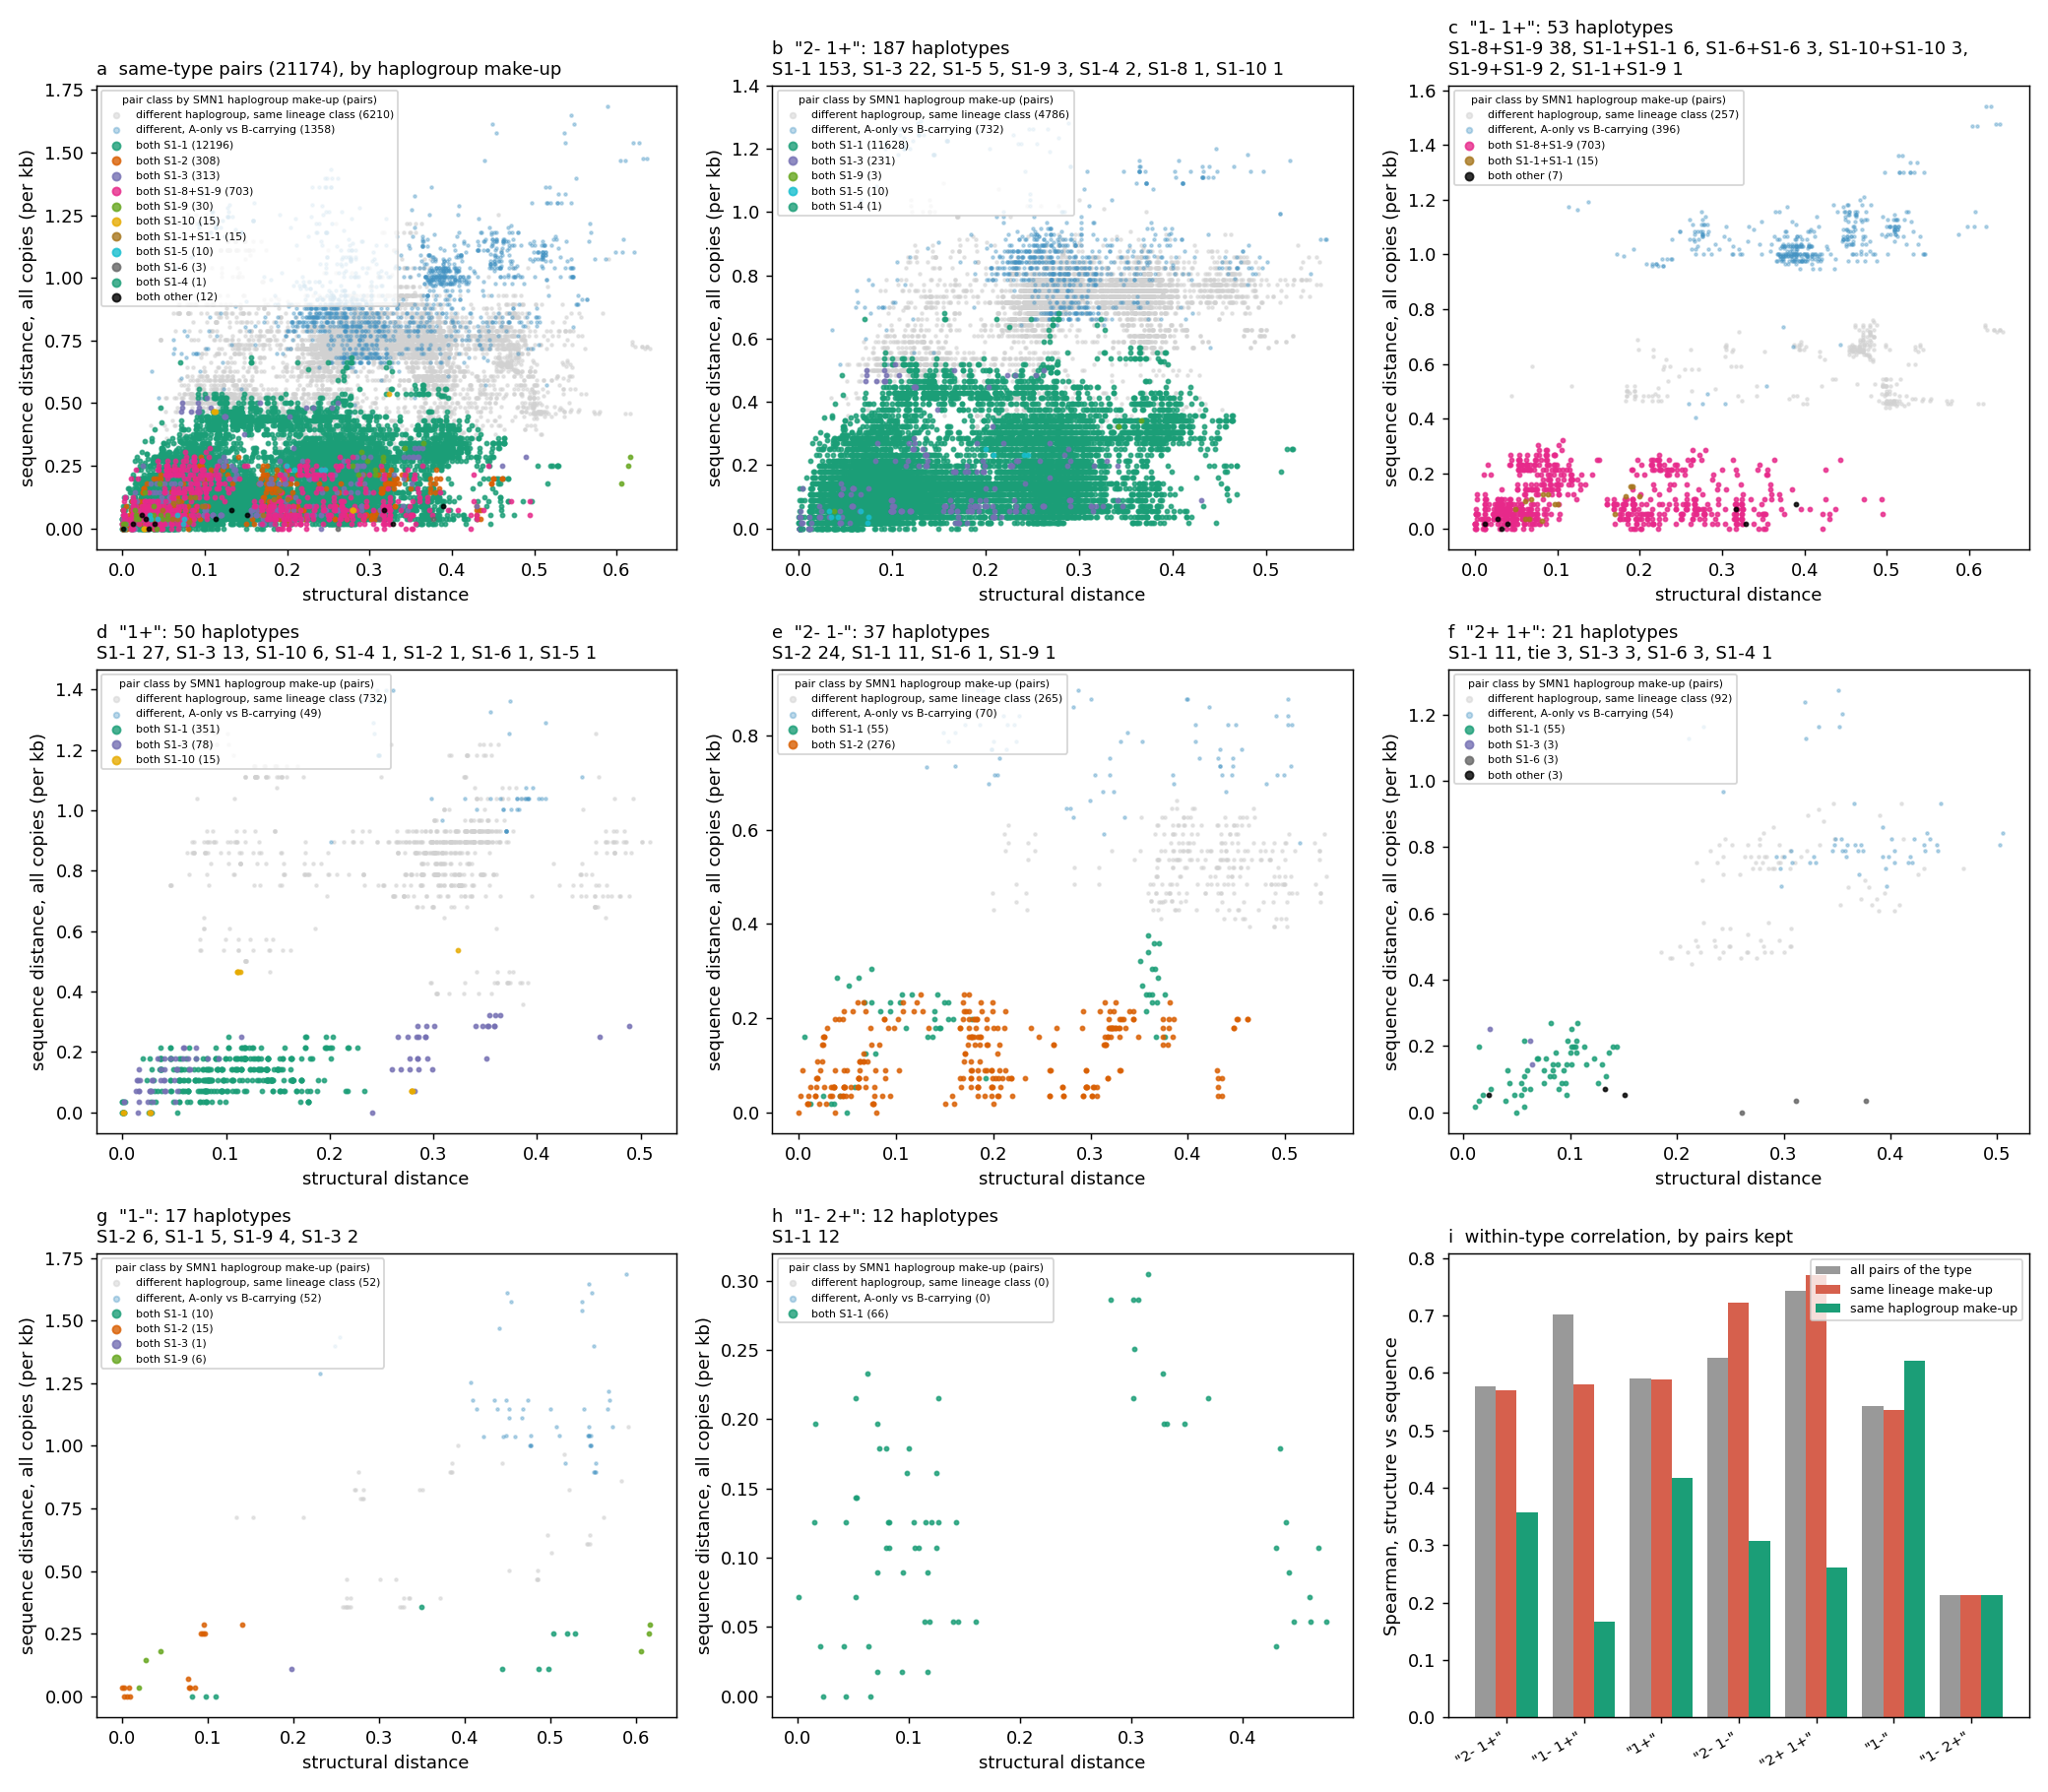
\includegraphics[width=\linewidth]{../figures/hap_scatter_hg.png}
\caption{Pairs of haplotypes of the same arrangement type, by structural distance (x) and sequence distance of all
their SMN copies (y, differences per kb), colored by SMN1 haplogroup make-up: a color, both haplotypes have that
make-up; light gray, different make-ups within one lineage class; blue, one haplotype carries only A copies and the
other a B copy. \textbf{a}, all \hsPairs{} same-type pairs; \textbf{b--h}, one panel per type with ten or more
haplotypes, titled with its make-ups and their counts. \textbf{i}, within-type rank correlation of structure and
sequence over all pairs of the type, over pairs of the same lineage make-up, and over pairs of the same haplogroup
make-up. Drawn by \texttt{26\_scatter\_lineage\_haplogroup.py}.}
\label{fig:hgscatter}
\end{figure}

\section{SMN1 lineages A and B, and the sub-lineages B1 and B2}\label{sec:lineages}
\subsection{The lineages are the two halves of the maximum-likelihood tree}\label{sec:apart}
Lineages are defined on the maximum-likelihood tree of the gene body (Section~\ref{m:lineages}, Fig.~\ref{fig:mltree};
step \texttt{05\_\allowbreak lineages.py}). Rooted on the orangutan copy, the human copies form one clade whose two child clades
are the two halves: \emph{lineage B} is the SMN1 copies of the half that holds the \cpe{} copies (\linB{} SMN1 copies
and \mlBsideHtwentyone{} h21 copies, support \mlIsup), and \emph{lineage A} the SMN1 copies of the other half (\linA,
with every SMN2 copy; support \mlIIsup). Within B's half, exactly two clades have support $\ge$95
and lie in no larger such clade: \emph{B1} is the SMN1 copies of the one that holds the h21 copies (\linBone{} copies with
\mlBhH{} h21 copies, support \mlBhSup), and \emph{B2} the SMN1 copies of the other (\linBtwo{} copies, support
\mlEightSup); the \linBnone{} remaining B copies are in neither. The node that joins B1 and B2 alone (\mlBBjoinCopies{}
copies) has support \mlBBjoinSup: by p-distance B2 is nearer A (\gsABtwo{} differences per kb) than it is to B1
(\gsBoneBtwo; Section~\ref{sec:grpdist}).

\subsection{Lineage B is exactly Chen et al.'s S1-6, S1-8 and S1-9 haplogroups (Table~\ref{tab:chenhg})}\label{sec:chenhg}
Our copies were matched to Chen et al.'s haplogroups~\cite{chen2023} by two independent routes (step
\texttt{11\_chen\_\allowbreak haplogroups.py}). Chen et al.'s ``haplotype'' is one gene copy (one SMN1 or SMN2 sequence), not a
chromosome. Chen et al.\ defined their haplogroups by reading monophyletic groups off a neighbor-joining tree of
such copies, and Paraphase assigns a new copy to the haplogroup of the most similar representative sequence; here copies are
assigned from their variant table.

\textbf{Copy by copy:} their supplementary Table S6 lists the variants shared within each haplogroup
(\hgSixVar{} variants, \hgSixSnv{} of them single-base, on GRCh38). \hgPlaced{} of the single-base ones fall inside the
aligned copies (\hgPlacedOne{} on the SMN1 locus, \hgPlacedTwo{} on the SMN2 locus), and the GRCh38 base at every one
is the reference base the table gives. Each SMN1 copy was genotyped at these sites and given the haplogroup whose
variant set it matches best: the Jaccard index of the copy's alternative bases and the haplogroup's listed variants,
at the sites where the copy has a base. Ties are kept (\hgTied{} of the \hgCopies{} SMN1 copies, \hgWithinTie{} of them between
subgroups of one family). The lead of the best haplogroup over the next has a median of \hgMarginB{} for B copies and
\hgMarginA{} for A copies, so the calls among the A haplogroups are the less certain.

\textbf{Person by person:} for the \hgPeople{} people in both Chen et
al.'s Table S3 and our tree, our lineage counts were set against the haplogroup names their method gave.
\begin{itemize}
\item \textbf{B is S1-6, S1-8 and S1-9; A is everything else.} B1 holds all \hgNineB{} copies of the S1-9 family
(S1-9 \hgNinePB, S1-9c \hgNineCB, S1-9d \hgNineDB) and \hgBoneSix{} of the \hgSixB{} S1-6 copies; B2 holds all
\hgEightB{} S1-8 copies; the \hgBnoneSix{} B copies in neither clade are S1-6. No copy of these three haplogroups is in
A, and every other haplogroup (S1-1 to S1-5, S1-10) is in A only. The worst B match has a Jaccard index of
\hgBMinJac{}, and no B copy is tied between haplogroups.
\item \textbf{The marker:} \hgMkNine{} S1-9 copies and \hgMkEight{} S1-8 copies carry \cpe, and no other copy
(Section~\ref{sec:marker}).
\item \textbf{SMN2's nearest SMN1:} the S1-10 copies are the A copies nearest SMN2 (mean \hgTenToTwo{} differences
per kb, against \hgAToTwo{} for all A), as Chen et al.\ found; S1-9 copies are \hgNineToTwo{} from SMN2.
\item \textbf{Person by person:} our B count equals the person's number of S1-6, S1-8 and S1-9 copies in all
\hgPeopleNineSix{} people.
\end{itemize}
\hgWithinTie{} A copies tie between S1-2 and S1-2c, which differ only downstream of the gene, and \hgTieA{} A copies
match no haplogroup better than another; neither touches the A/B question. The lineage split is therefore not a new
grouping: it is the deepest division among Chen et al.'s haplogroups, and their common African two-copy allele
(S1-8 with S1-9d) is a B2 copy with a B1 copy. What the assemblies add is where those copies sit
(Section~\ref{sec:posstrand}).

\begin{table}[htbp]\small\centering
\caption{SMN1 copies of each Chen et al.\ haplogroup family (by the copy-level match) in lineages A and B, how many
carry \cpe, and their mean distance to the SMN2 copies (differences per kb). Families: S1-1 includes S1-1c, and so
on. ``tie'': equally good matches across families. Written by \texttt{40\_numbers.py} from
\texttt{results/sv/chen\_hg\_copies.tsv}.}\label{tab:chenhg}
\begin{tabular}{@{}lrrrr@{}}\toprule
Haplogroup family & A & B & \cpe{} & To SMN2\\\midrule
\tabChenHg
\bottomrule\end{tabular}
\end{table}

\subsection{B1 is the copy group furthest from SMN2, and B2 lies nearer A than it does to B1 (Fig.~\ref{fig:grpdist}, Table~\ref{tab:grpdist})}\label{sec:grpdist}
Every pair of copies among lineage A (\linA{} copies), lineage B (\linB) and SMN2 (\gdNTwo), with the \gdNHtw{} h21
hybrids beside them, is compared over the same \nGeneCols{} gene-body columns (Section~\ref{sec:compared}), counting
differences over the bases both copies have (on average \gdBases{} per pair; step \texttt{10\_group\_distances.py}).
The same comparison with B split into B1 and B2 is in \texttt{results/sv/group\_pair\_distances\_sub.tsv}.
\begin{itemize}
\item \textbf{Within each group} (differences per kb, mean): B2 is the most uniform (\gsBtwoBtwo), then B1
(\gsBoneBone), A (\gsAA) and SMN2 (\gdTwoTwoMean). B as a whole is \gdBBMean, because it holds two sub-lineages
\gsBoneBtwo{} apart.
\item \textbf{A against SMN2} is the closest pair of the three groups: mean \gdATwoMean{} (\gdATwoDiffs{} differences per
pair), range \gdATwoMin--\gdATwoMax; \gdATwoBelow\% of these pairs are closer than the 95th percentile of
within-group distances.
\item \textbf{A against B}: mean \gdABMean{} (\gdABDiffs{} differences), range \gdABMin--\gdABMax; by sub-lineage A is
\gsABtwo{} from B2 and \gsABone{} from B1, so B2 is nearer A than it is to B1 (\gsBoneBtwo).
\item \textbf{B against SMN2} is the furthest: mean \gdBTwoMean{} (\gdBTwoDiffs{} differences), B1 \gsBoneTwo{} and B2
\gsBtwoTwo; the closest B--SMN2 pair (\gdBTwoMin) is further apart than the median A--SMN2 pair (\gdATwoMed), and
\gdBTwoBelowFine\% of B--SMN2 pairs are closer than the 95th percentile of within-group distances (shown as 0\% in
Table~\ref{tab:grpdist} after rounding).
\item \textbf{Copy by copy} (Fig.~\ref{fig:grpdist}c,d): no B copy is on average nearer SMN2 than the other B copies
(\gdBNearTwo{} of \linB), \gdBNearA{} is nearer A, and no SMN2 copy is nearer A than SMN2 (\gdTwoNearA{} of \gdNTwo).
No A copy is nearer B than A (\gdANearB), and \gdANearTwo{} (\gdANearTwoHap) is nearer SMN2 than A.
\item \textbf{h21} hybrids are on average nearest SMN2 (\gdTwoHtwMean), then B (\gdBHtwMean) and A (\gdAHtwMean);
their wide spread (within h21 up to \gdHtwHtwMax) fits copies that mix the two genes.
\end{itemize}
By raw difference counts, then, A and SMN2 are the nearest pair, and B1 is the group furthest from SMN2. These counts do
not say why: shared ancestry, or gene conversion between A and SMN2 copies, would give the same pattern
(Section~\ref{sec:history}). Distances are p-distances, uncorrected for repeated changes at one site; every
difference counts once (a long insertion counts as many); pairs share copies and are not independent, so the ranges
and shares are descriptive.

\begin{figure}[htbp]\centering
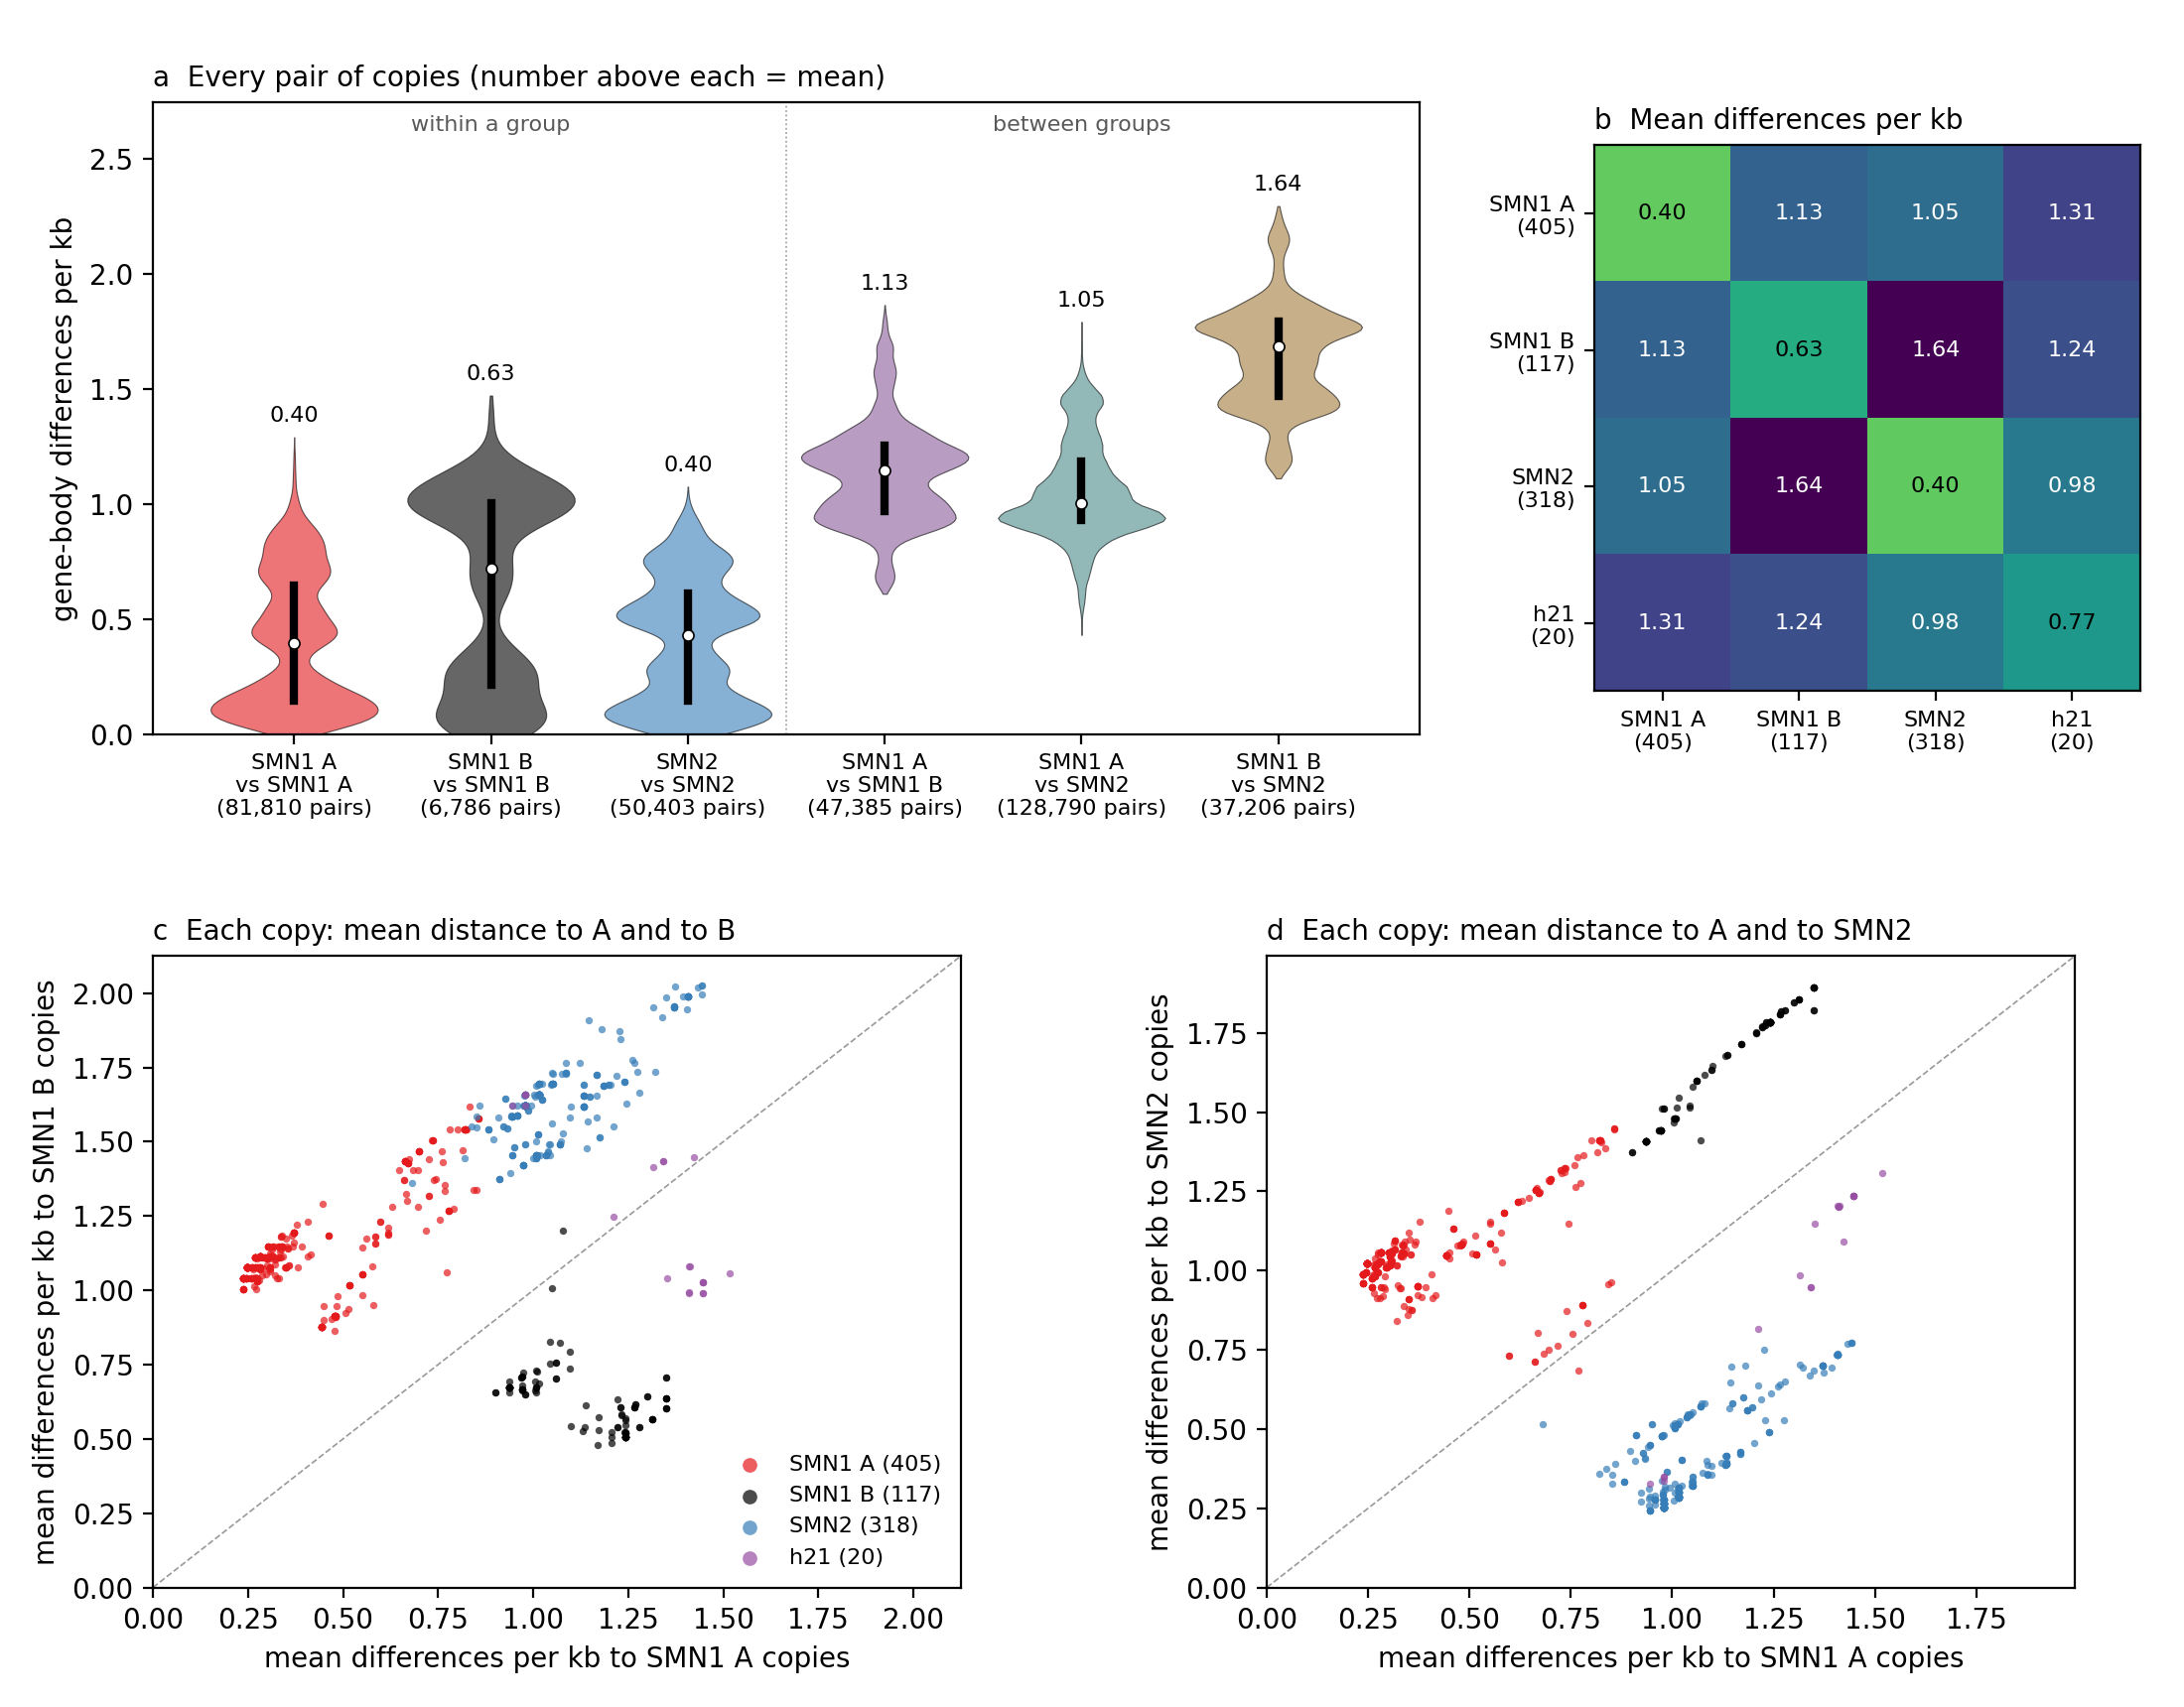
\includegraphics[width=\linewidth]{../figures/group_distances.png}
\caption{Gene-body distances between every pair of copies of SMN1 lineage A (red), SMN1 lineage B (black) and SMN2
(blue), with h21 hybrids (purple); colors as in Figs.~1--5. \textbf{a}, distribution of the distance over all pairs within each group and
between each pair of groups (violin; bar, interquartile range; dot, median; number, mean; pair counts under each).
\textbf{b}, mean distance for every pair of groups, h21 included. \textbf{c}, each copy's mean distance to the A
copies against its mean distance to the B copies; \textbf{d}, the same against the SMN2 copies (a copy's distance to
itself left out); dashed line, equal distance. B is not split into B1 and B2 here. Drawn by
\texttt{10\_group\_distances.py} from \texttt{results/sv/copies.aln.fa}.}
\label{fig:grpdist}
\end{figure}

\begin{table}[htbp]\small\centering
\caption{Gene-body distance between copies, differences per kb, for every pair of groups: pairs compared, mean,
median, 5--95th percentile, range, mean differences per pair; for pairs of different groups, the net distance (mean
minus the average of the two within-group means) and the \% of pairs closer than the larger of the two within-group
95th percentiles. Written by \texttt{40\_numbers.py} from \texttt{results/sv/group\_pair\_distances.tsv}.}\label{tab:grpdist}
\begin{tabular}{@{}lrrrrrrrr@{}}\toprule
Groups & Pairs & Mean & Median & 5--95\% & Range & Diffs & Net & \% within\\\midrule
\tabGrpDist
\bottomrule\end{tabular}
\end{table}

\subsection{Two sites separate A from B in every copy; none lies in the coding sequence (Fig.~\ref{fig:absites})}\label{sec:absites}
The lineages differ at \abCols{} gene-body columns, where the commonest state in A differs from the commonest state in B
(a gap counts as a state). Adjacent columns of one insertion or deletion merge into one event, leaving \abEvents{}
events: \abSNV{} base changes and \abIndel{} insertions or deletions (step \texttt{23\_ab\_sites.py}).
\begin{itemize}
\item \textbf{How cleanly they separate.} The \emph{separation} of an event is the share of copies carrying their own
lineage's state, taken in the lineage where that share is lower. At \abNearFixed{} events it is at least 90\%
(\emph{near-fixed}), and at \abPerfect{} it is 100\% (no copy of either lineage carries the other state):
chr5:\abPerfOnePos{} (\abPerfOneKind{} in the 5$'$ untranslated part of exon~1, \abPerfOneC; A's base on
\abPerfOneA{} of \linA{} A copies, B's on \abPerfOneB{} of \linB{} B copies) and chr5:\abPerfTwoPos{}
(\abPerfTwoKind{} in intron~1; \abPerfTwoA{} and \abPerfTwoB).
\item \textbf{Where.} Most events lie in intron~1 (\abIntronOne) and intron~6 (\abIntronSix); \abExonEvents{} touch an
exon, the one in exon~1 above and c.*211\_*212del in the 3$'$ untranslated part of exon~8. None lies in the coding
sequence.
\item \textbf{SMN2.} At \abTwoA{} events SMN2 carries A's state and at \abTwoB{} B's, which fits A and SMN2 being the
nearest pair (Section~\ref{sec:grpdist}), though these sites are only part of that distance.
\end{itemize}
The \evAB{} sites of the history (Section~\ref{sec:history}) are the near-fixed events less the one insertion or
deletion among them, since the ape bases are read at single-base sites. The lineages were cut from a tree built on this same alignment, so how cleanly a site separates
them is partly built in; copies outside the tree, or reads, would be needed to test these sites as lineage markers.

\begin{figure}[htbp]\centering
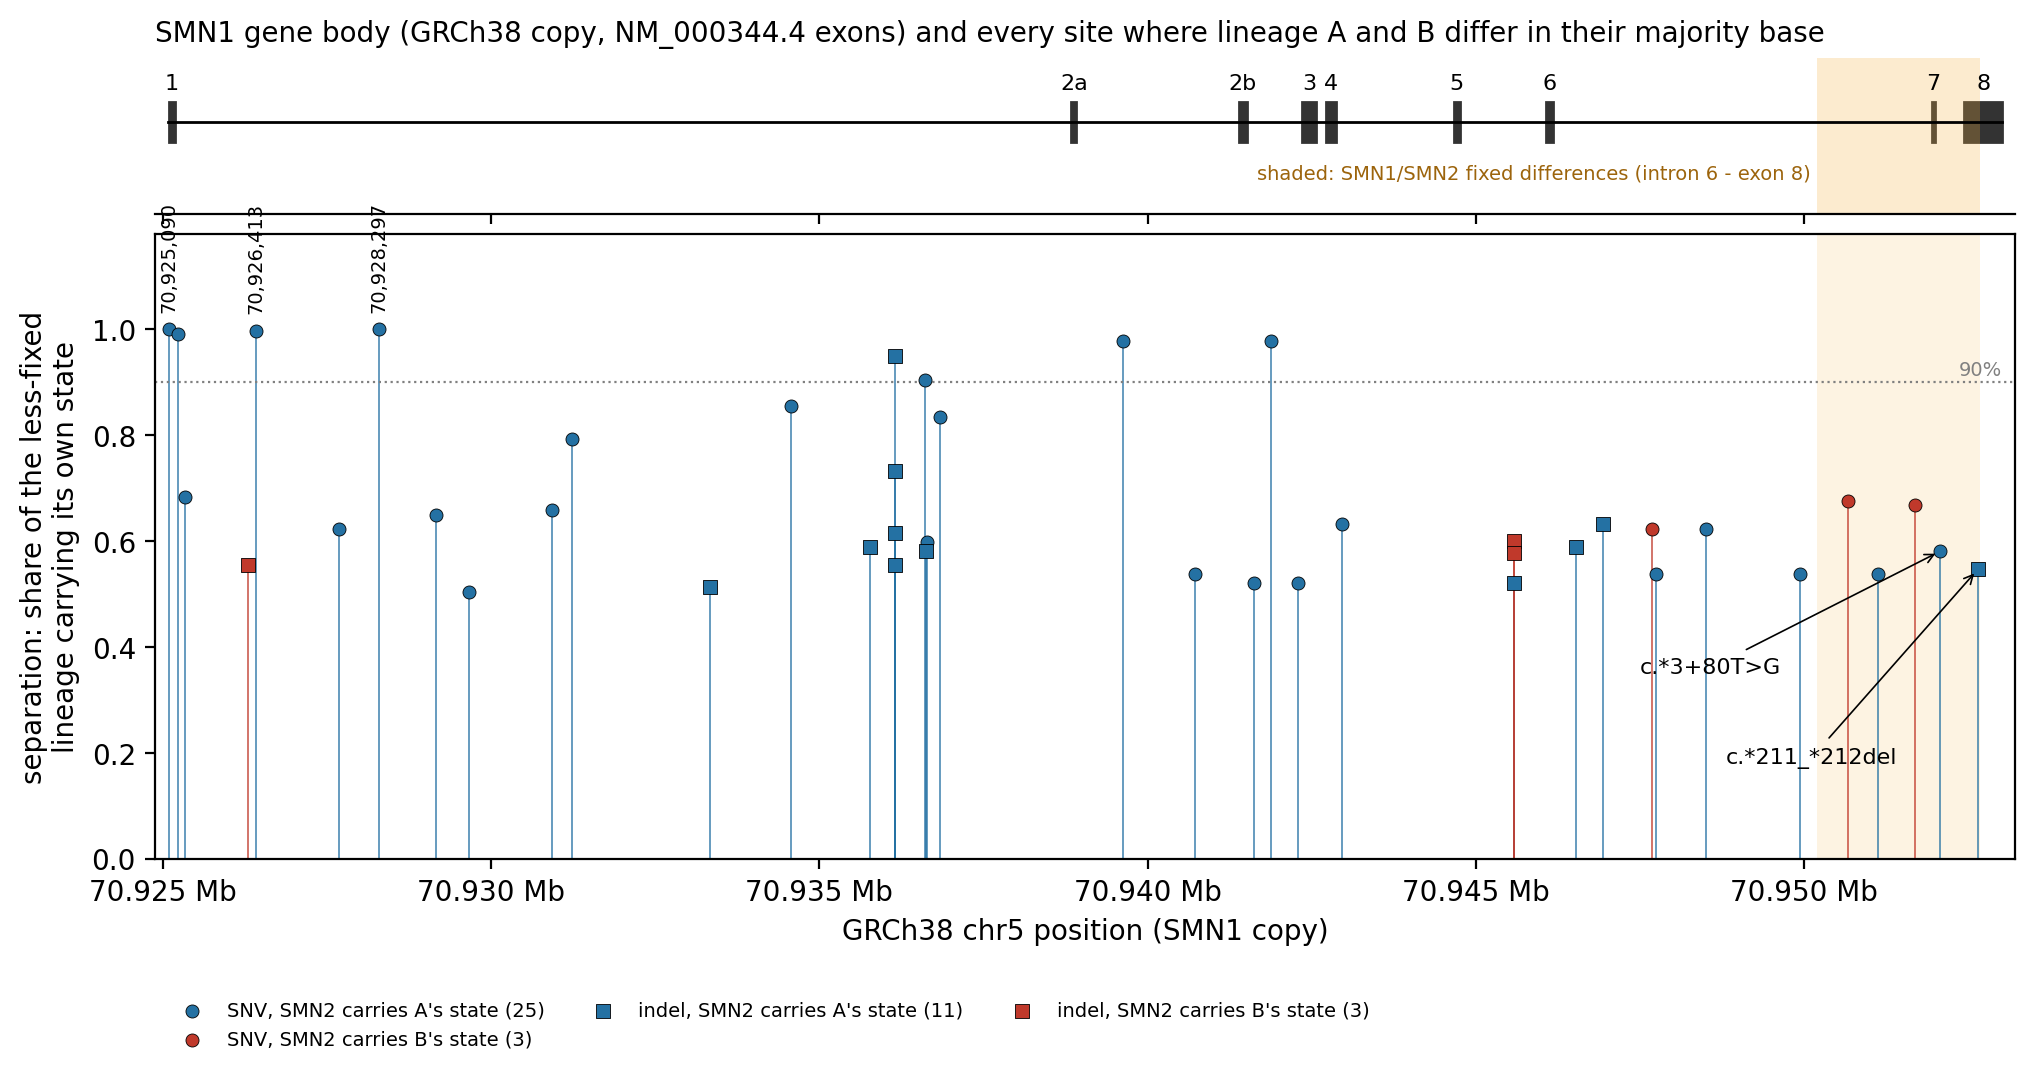
\includegraphics[width=\linewidth]{../figures/ab_sites.png}
\caption{Every gene-body site where the commonest state of lineage A differs from that of lineage B, drawn along the
SMN1 gene (GRCh38 chr5 coordinates) over the exons of NM\_000344.4: base changes and insertions or deletions, their
height the separation (share of the less-fixed lineage carrying its own state), colored by whose state SMN2 carries;
\cpe{} and c.*211\_*212del are labeled. Drawn by \texttt{23\_ab\_sites.py} (\texttt{results/sv/ab\_sites.tsv},
\texttt{results/sv/ab\_site\_events.tsv}).}
\label{fig:absites}
\end{figure}

\subsection{The duplication marker c.*3+80T>G tags B1 and part of B2}\label{sec:marker}
\cpe{} lies in intron~7, 80 bases after the end of exon~7 (chr5:70{,}952{,}074 on the GRCh38 SMN1 copy), so it does not
change the protein. Luo et al.\ sequenced \emph{SMN1} in Ashkenazi Jewish and African American carriers of duplication
alleles and reported six variants on the major Ashkenazi duplication allele: g.27134T>G in intron~7 (\cpe{}) and
g.27706\_27707delAT in exon~8 (c.*211\_*212del), which in every case they examined lay together on one \emph{SMN1} copy, and
four changes in introns~1, 2a and~6 found with them in both groups. g.27134T>G was on 49 of 99 Ashkenazi duplication
carriers, and on duplication alleles in every group they tested, though specific to them only in their Asian
sample; finding it in a person with two \emph{SMN1} copies sharpens the residual risk of being a silent 2+0
carrier~\cite{luo2014}. Later assays genotype the two with copy number~\cite{feng2017,milligan2021,mikhalchuk2025}.
Luo et al.'s Table~4 gives GRCh37 positions. Shifted by \luoShift{} bases, the shift that puts their exon-8 deletion at
c.*211 of the GRCh38 copy and at which each of their reference bases is the GRCh38 base, five of the six fall on
lineage B1 (step 23b, \texttt{results/sv/luo\_variants.tsv}): each is on \luoBoneLo--\luoBoneHi{} of the \linBone{} B1
copies and on no A or SMN2 copy, while B2 carries only the intron-7 change (\luoBtwoMk{} copies, without the
deletion), so here the two do not always travel together. The sixth, an intron-1 G>T at the end of a run of G next to
the run of 14 T that ends at \rdUnresSite{} and leaves one A/B site unresolved in the apes (Section~\ref{sec:history}), is on no copy as written; \luoIntronOneB{} B1 copies carry that run of G
shortened by one base at its other end, which may be the same change placed differently, and we leave it open. The
duplication haplotype Luo et al.\ described is thus, as far as these sites show, the haplotype of B1.
It tags only some duplication alleles: Chen et al.\
report that it carries a silent-carrier risk of 1.7--3.0\%, against 88.5\% for the S1-8 with S1-9d haplogroup pair, and
Mikhalchuk et al.\ found it in a small share of Russian duplication carriers~\cite{chen2023,mikhalchuk2025}. Here it is
on \linBoneMk{} of the \linBone{} B1 copies, \linBtwoMk{} of the \linBtwo{} B2 copies and no A copy: it marks
sub-lineage B1 nearly completely and B2 only in part, so a two-copy allele made of B2 copies, or a B1 copy without it,
is missed.

\subsection{Copy order and strand: A is telomeric, B1 centromeric and reversed, B2 telomeric and forward}\label{sec:posstrand}
A \emph{copy} is one SMN gene in the window: an SMN1, SMN2, hybrid (h12, h21) or $\Delta$7--8 copy (Section~\ref{sec:compared}). A copy's \emph{copy order} is which of the window's SMN genes it is, all of them
counted, from the centromeric end: \emph{centromeric} is the first copy from the centromeric end, \emph{telomeric} the last, \emph{middle} any
between, and \emph{single} the only SMN copy of the window. Copy order is counted over the whole window, so it is not the same as the cenSMN and telSMN slots of the arms of the \RU{A} pair (Section~\ref{sec:palindrome}); it is read on resolved haplotypes only. The main text and Fig.~\ref{fig:mltree} group copies by arm instead (Section~\ref{m:cen}); on the haplotypes with the pair the two agree, \coCenFirst{} of the \coCenN{} cenSMN-arm copies being first by copy order and \coTelLast{} of the \coTelN{} telSMN-arm copies last, while copy order also places the copies of haplotypes without the pair. A copy's
\emph{strand} is its orientation on the GRCh38-oriented window. Both are labels taken from the assembly, outside the
sequence comparison: every copy went into the alignment on the SMN1-gene strand, so neither label can shape the tree,
and an association between them and the lineages is not built in.

\textbf{The copies behind the counts.} Of the \linA{} A copies, \linACen{} are centromeric, \linATel{} telomeric (the
\linRef{} reference copies of GRCh38 and CHM13 among them, both forward), \linASingle{} single, \linAMid{} middle, and
\linAUnres{} sit on unresolved haplotypes and have no copy order. Of the \linB{} B copies, \linBCen{} are centromeric,
\linBTel{} telomeric and \linBSingle{} single, so none is a middle copy or on an unresolved haplotype; B1 is \linBoneCen{} centromeric, \linBoneTel{} telomeric and
\linBoneSingle{} single, and B2 \linBtwoCen{} centromeric and \linBtwoTel{} telomeric. The copy-order test below uses
the \linPosN{} centromeric and telomeric copies.

\textbf{Copy order.} A is telomeric in \linATel{} copies against \linACen{} centromeric. B as a whole is found in both
places, but its sub-lineages are not: B1 against B2, centromeric against telomeric, two-sided Fisher exact
$p=$\,\linSubPpos. On the \linMixHaps{} haplotypes with one B1 and one B2 copy (all ``1-~1+'', \linMixAfr{} of them
AFR), B1 is centromeric and reversed on \linMixBoneCenRev{} and B2 telomeric and forward on \linMixBtwoTelFwd.

\textbf{Strand mostly follows copy order, with one exception.} Every centromeric B1 copy is reversed (\linBoneCenRev{} of
\linBoneCen) and every telomeric B2 copy forward (\linBtwoTelFwd{} of \linBtwoTel). In A, \linACenRev{} of the
\linACen{} centromeric copies are reversed, and \linATelFwd{} of the \linATel{} telomeric copies forward: the first
copy of a head-to-head inverted pair reads reversed and the last forward. The exception is the \linATelRev{} telomeric
A copies that are reversed: \linATelRevTwoMOneM{} of them are on ``2-~1-'' and \linATelRevTwoPOneM{} on ``2+~1-''
haplotypes, where the SMN1 copy is not the forward member of a head-to-head pair. \linATelRevBand{} of them lie on the \linBandTwoN{} haplotypes of the S1-2 band
(Section~\ref{sec:bands}), one on each.

\textbf{How far to trust it.} Copy order does not define a lineage: \linBoneTel{} B1 copies are telomeric, \linBtwoCen{}
B2 copies centromeric, and \linACen{} A copies centromeric. \linBAfr{} of the \linB{} B copies are from AFR donors
(outside AFR, \linBNonAfrPops), so the association is mixed with ancestry and cannot be tested elsewhere. The Fisher
test treats copies as independent, though two copies of one haplotype, and haplotypes of one person, are not.

\subsection{Lineage B in populations, haplotypes and arrangements (Fig.~\ref{fig:lindetail}, Tables~\ref{tab:lincomp}--\ref{tab:linpop})}\label{sec:lindetail}
Every count here is a cross-tabulation written by \texttt{06\_lineage\_detail.py} or \texttt{40\_numbers.py}, with the
caveats above (assembled bases only, copies not independent).

\textbf{Where B occurs.} B copies are found in all \ldAfrPopsB{} of the \ldAfrPops{} African-ancestry populations; in the
\ldAfrPopsBig{} with ten or more SMN1 copies they are \ldShareMin--\ldShareMax\% of SMN1 copies (Table~\ref{tab:linpop},
Fig.~\ref{fig:lindetail}c). Outside AFR the only B copies are \linBNonAfrPops{} SMN1 copies; none of the other
\ldNonAfrNoB{} non-AFR populations carries one. B is spread across African-ancestry populations, not confined to one.

\textbf{How B sits on a haplotype} (Table~\ref{tab:lincomp}). Of the \ldHaps{} haplotypes with an SMN1 copy in the tree,
\ldCompA{} carry a single A copy and \ldCompAA{} two A copies; \ldCompB{} carry a single B copy (\ldCompBAfr{} AFR) and
\ldCompBB{} two B copies (\ldCompBBAfr{} AFR), of which \linMixHaps{} are one B1 with one B2 and \linMkOneOne{} two B1
copies; only \ldCompAB{} carry one copy of each lineage. Among resolved AFR haplotypes, those with a B copy carry two
or more SMN1 copies far more often than those without (\ldTestBMulti{} of \ldTestBN{} against \ldTestNoBMulti{} of
\ldTestNoBN; Fisher $p=$\,\ldTestP; hybrids not counted as SMN1). The table counts every haplotype with an SMN1 copy in the tree, resolved or not; this test counts resolved
haplotypes only, so its denominators are smaller than the table's AFR columns.

\textbf{B by arrangement type} (Fig.~\ref{fig:lindetail}d). B is \ldOneOnePB{} of the \ldOneOnePN{} SMN1 copies of
``1-~1+'' haplotypes and \ldTwoOnePB{} of \ldTwoOnePN{} in the commonest type ``2-~1+''. Every SMN1 copy of a
``1-~h21$\pm$'' haplotype is B (\ldHtwoOneB{} of \ldHtwoOneN), beside a telomeric h21 hybrid; the tree also places
\mlBhH{} h21 copies in the B1 clade. So B goes with two structures: the inverted SMN1 pair ``1-~1+'' (B1 with B2) and
the SMN1 + h21 pair (B1 with h21).

\textbf{Downstream context.} The lineages barely differ: an SMN1-type downstream environment for \ldEnvOneB{} of
\ldEnvAssB{} B and \ldEnvOneA{} of \ldEnvAssA{} A copies with the environment read; full-length NAIP at the 3$'$ side
for \ldNaipFullB{} of \linB{} B and \ldNaipFullA{} of \linA{} A copies. B is a difference in the SMN1 gene body, not
in the unit around it.

\begin{figure}[htbp]\centering
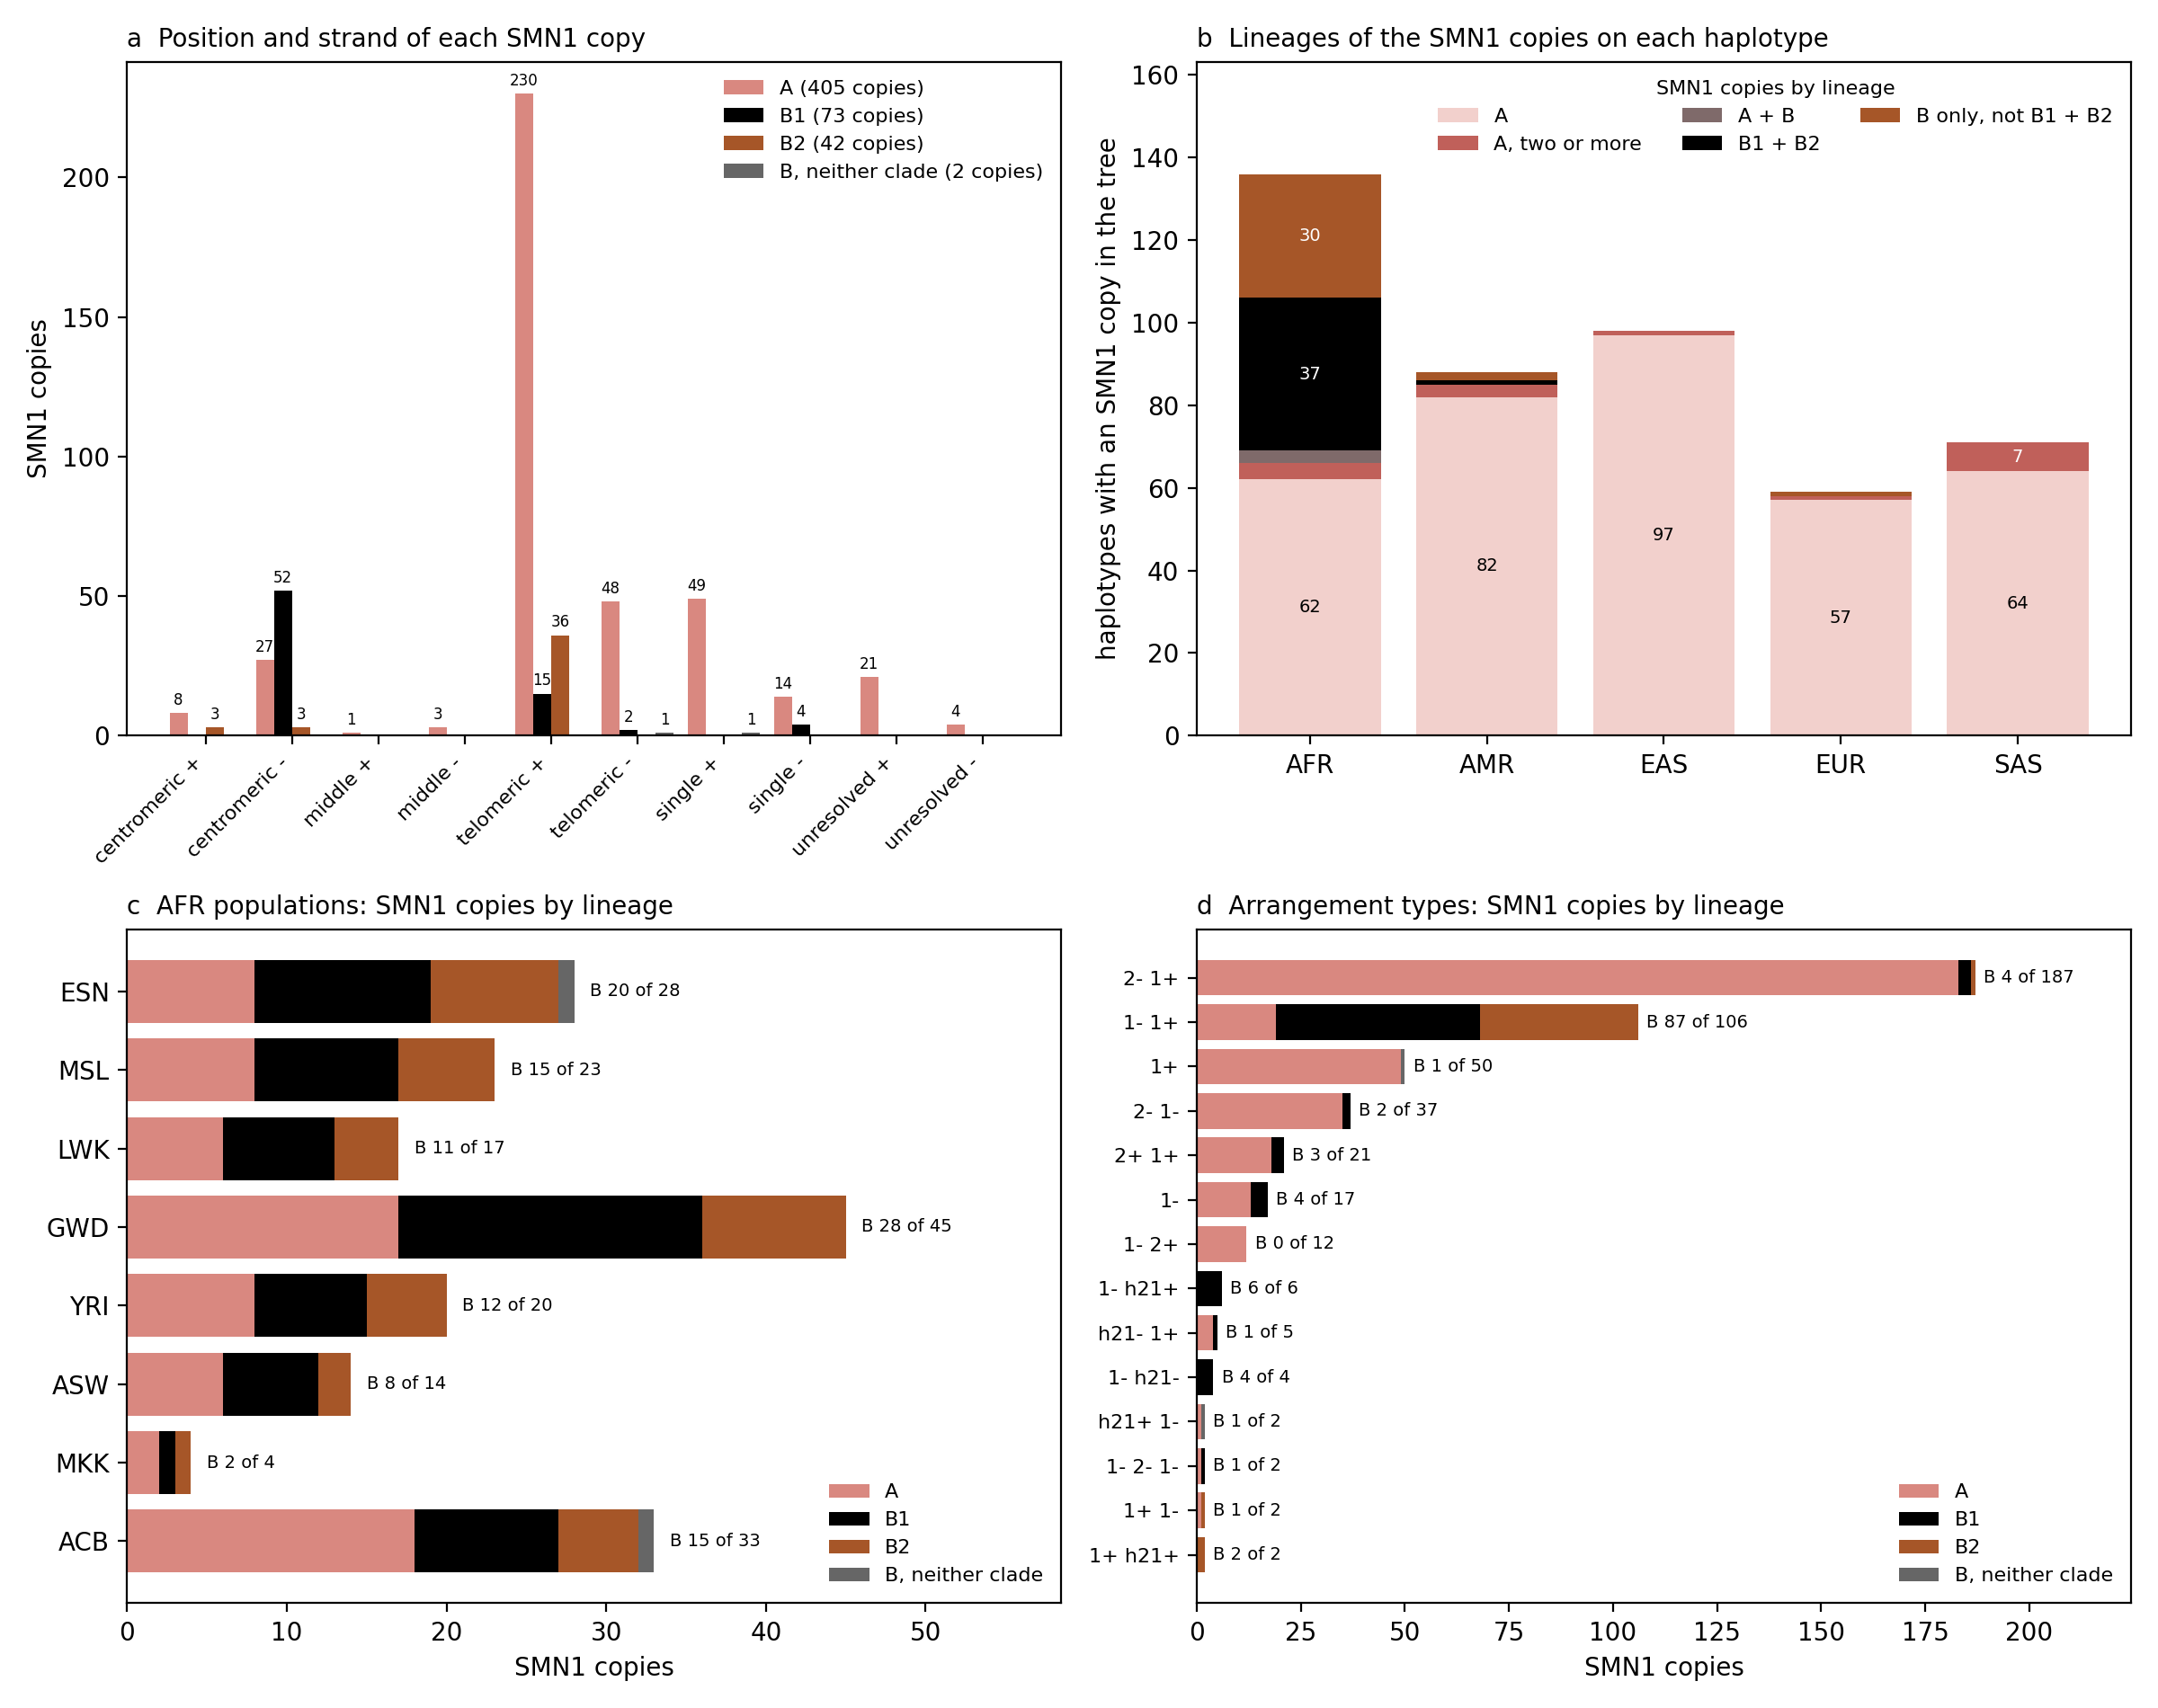
\includegraphics[width=\linewidth]{../figures/lineage_detail.png}
\caption{The two SMN1 lineages, with B split into its sub-lineages (colors as in Figs.~1--5: A red, \linA{} copies; B1 black; B2 brown; B in neither clade gray; \linB{} B copies in all).
\textbf{a}, each copy's copy order among the SMN copies of its haplotype and its strand on GRCh38 (``unresolved'': copy
on an unresolved haplotype, no copy order). \textbf{b}, haplotypes by the lineages of their SMN1 copies, per continental
group (one A copy; two or more A copies; A with a B copy; B1 with B2; one or more B copies, not B1 with B2). \textbf{c}, SMN1 copies by lineage in each African-ancestry population. \textbf{d}, SMN1 copies by lineage in
each arrangement type that holds a B copy or ten or more SMN1 copies. Drawn by \texttt{06\_lineage\_detail.py}.}
\label{fig:lindetail}
\end{figure}

\begin{table}[htbp]\small\centering
\begin{minipage}[t]{0.47\linewidth}\centering
\caption{Haplotypes by the lineages of their SMN1 copies (A; B1, B2; B (n.c.): a B copy in neither sub-clade), per
continental group; ``other'': haplotypes outside the five groups and the reference haplotypes. Written by \texttt{40\_numbers.py} from
\texttt{results/sv/marker\_lineage.tsv}.}\label{tab:lincomp}
{\setlength{\tabcolsep}{3pt}\begin{tabular}{@{}lrrrrrrr@{}}\toprule
& AFR & AMR & EAS & EUR & SAS & other & total\\\midrule
\tabLinComp
\bottomrule\end{tabular}}
\end{minipage}\hfill
\begin{minipage}[t]{0.47\linewidth}\centering
\caption{SMN1 copies by population: all copies, B copies, B as \% of SMN1 copies. The last row pools the AMR, EAS, EUR and SAS populations not listed, and ASL, which has no superpopulation label. The rows hold \ldPopRowsN{} of the \ldPopAllN{} SMN1 copies; the 2 reference copies (GRCh38, CHM13) and the \ldPopNoLabN{} copies of the two donors with no population label (HG005, HG002\_Q100; all lineage A) are not in it. MKK is the Maasai in Kinyawa, Kenya. Written by \texttt{40\_numbers.py}
from \texttt{results/sv/lineage\_population.tsv}.}\label{tab:linpop}
\begin{tabular}{@{}lrrr@{}}\toprule
Population & SMN1 & B & \% B\\\midrule
\tabLinPop
\bottomrule\end{tabular}
\end{minipage}
\end{table}

\subsection{A copy's distance to SMN2 goes mainly with its lineage; where an A copy sits shifts it a little}\label{sec:distctx}
For each SMN1 copy, \texttt{17\_distance\_context.py} takes its mean gene-body distance to the SMN2 copies and compares
it, within each lineage, across where the copy sits (medians, differences per kb; Mann--Whitney or Kruskal--Wallis
tests, descriptive only, since copies are not independent; donor copies only, so the two reference SMN1 copies are
left out). The main text gives these tests by arm (Section~\ref{m:cen}); here they are given by copy order and by whether the copy is on an arm of the palindrome.
\begin{itemize}
\item \textbf{In A, centromeric and telomeric copies are equally far.} Centromeric A copies are \dcACen{} from SMN2
(\dcACenN{} copies) and telomeric ones \dcATel{} (\dcATelN); across centromeric, telomeric and single copies the
distributions differ (Kruskal--Wallis $p=$\,\dcPAPos), from the single copies, which sit slightly further (\dcASingle).
\item \textbf{In A, the palindrome and the arrangement shift it a little.} A copies on an arm of the \RU{A} palindrome
are \dcAPalYes{} from SMN2 (\dcAPalYesN{} copies) and those elsewhere \dcAPalNo{} (\dcAPalNoN; $p=$\,\dcPAPal); across
the arrangement types with ten or more A copies the medians run from \dcAArrMin{} to \dcAArrMax{} ($p=$\,\dcPAArr).
These shifts are clear but small next to the gaps between
lineages (Section~\ref{sec:grpdist}).
\item \textbf{In B, copy order reflects the sub-lineage.} Centromeric B copies are \dcBCen{} (\dcBCenN) and telomeric
ones \dcBTel{} (\dcBTelN; $p=$\,\dcPBPos; within AFR \dcAfrBCen{} against \dcAfrBTel, $p=$\,\dcPAfrBPos). Centromeric B
copies are mostly B1 and telomeric ones mostly B2, and B1 is further from SMN2 than B2 (Section~\ref{sec:grpdist}).
Either way a B copy is further from SMN2 than any group of A copies.
\item \textbf{The palindrome does not set it.} B copies on an arm of the \RU{A} palindrome are \dcBPalYes{}
(\dcBPalYesN{} copies, the \palSmnB{} B copies of Section~\ref{sec:palindrome} and that of \palNoCopyHap, whose \RU{A} pair holds no telSMN copy) from SMN2, those elsewhere \dcBPalNo{} (\dcBPalNoN; $p=$\,\dcPBPal).
\item \textbf{The downstream unit, a hint in B.} B copies in an SMN1-type downstream environment are \dcBEnvOne{} from
SMN2 (\dcBEnvOneN{} copies); in a mixed environment \dcBEnvMixed{} (\dcBEnvMixedN) and in an SMN2-type one \dcBEnvTwo{}
(\dcBEnvTwoN; $p=$\,\dcPBEnv). With so few copies in the last two this is a hint only.
\end{itemize}
\textbf{Speculation (untested).} B1 may have become distant from SMN2 while it sat where it exchanged less sequence with
SMN2 copies. Today's copy positions cannot test this: the distance goes mainly with the lineage and sub-lineage, and where
a copy now sits shifts it by little. A dated tree and the junction sequences between paired copies would be the place to start.

\section{The \RU{A} palindrome: one SMN copy per arm, at mirror positions}\label{sec:palindrome}
Are SMN1 and SMN2 at the center of a palindrome of large repeat units (Fig.~\ref{fig:allhaps})? From the repeat units
\texttt{pangea cohort bundle repeat-units} found (\path{results/decomp/smn.repeat_units.tsv}) and the copies placed in
them, \texttt{13\_palindrome.py} looks for an adjacent inverted pair of \RU{A} units on each of the \palHaps{}
resolved haplotypes with repeat units (the other \palNoUnits{} resolved haplotypes, each with one SMN copy, have no
recurring bundle apart from the tandem-array bundle and so no unit; GRCh38, kept by the step as a reference row, is not counted).
\begin{itemize}
\item \textbf{The core is a near-symmetric palindrome.} \palAdj{} haplotypes carry an adjacent inverted \RU{A} pair:
\palHead{} head to head (\RU{A}+ \RU{A}$-$) and \palTail{} tail to tail (\RU{A}$-$ \RU{A}+; \palTailHaps, arrangements \palTailArr, each
with at most one SMN copy on either side). Of the head-to-head pairs, \palPair{} carry an SMN copy on each arm; the other
(\palNoCopyHap) has none on its telomeric arm. Those \palPair{} are the palindrome of this section, and every arm
length and copy distance is measured from their \RU{A}+ \RU{A}$-$ junction. The two \RU{A} units are a median \palArmL{} and
\palArmR{} kb long (median difference \palArmDiff{} kb), separated by a median \palGap-kb stretch no unit covers (the short one of the two clusters of Section~\ref{m:arr} is nearly always on a haplotype whose cenSMN arm carries X, \palGapShortCOne{} of \palGapShortN{} C1 against \palGapLongCOne{} of \palGapLongN{} for the long one, Fisher $p=$\,\palGapTypeP, as where a unit ends is set by what follows the core; Section~\ref{m:arms}); the axis S
lies next to it inside one of the \RU{A} units, and inside no unit of another family, on \palSinA{} of the \palGapSN{} copies of S at the axis (on \palGapSHaps{} haplotypes).
They include \palTwoOne{} ``2-~1+'' and \palOneOne{} ``1-~1+'' haplotypes.
\item \textbf{The SMN copies sit on the arms, at mirror positions, not at the center.} Every one of the \palPair{}
haplotypes has an SMN copy on each arm (\palCopies{} items, one counted copy per arm plus one truncated piece, so \palThreeCopy{} haplotype has three items). They lie
\palDmin--\palDmax{} kb from the axis (median \palDmed{} kb); the nearest copies on the two arms differ in their
distance from the axis by a median \palMirror{} kb. Inside its own \RU{A} unit a copy sits \palRelMin--\palRelMax\% of the
way from the unit's 5\(^\prime\) end (median \palRelMed\%; \palInUnit{} copies inside one \RU{A} unit), close to that end.
This is why paired copies lie about twice \palDmed{} kb apart. The truncated piece is on \palThreeHap.
\item \textbf{Beyond the core the units seldom mirror.} Of the \palRoom{} pair haplotypes with at least one more
unit on both sides, \palDeeper{} mirror one further pair (\palDeeperHap). The palindrome is the \RU{A} pair itself, not the whole region.
\item \textbf{What flanks the pair.} Family letters are those of Section~\ref{sec:compared}; families with fewer than ten occurrences are not in Table~\ref{tab:unitfam}. On the \palFlankN{} pairs, the unit next to \RU{A}+ on the centromeric side is
\palFlankLText; the unit next to \RU{A}$-$ on the telomeric side is \palFlankRText. An \RU{B} unit (mostly Xi$'$ and Xi,
Table~\ref{tab:unitfamel}) lies on both sides, \RU{B}$-$ before the pair and \RU{B}+ after it (often beyond an \RU{D}$-$ or \RU{E}+ unit), on
\palFlankBB{} haplotypes. These \RU{B} units face opposite ways but are not adjacent to the pair on both sides, so they are
not counted as a mirrored unit pair above.
\item The other \palNoPair{} haplotypes have no such palindrome (\palNoAdj{} have no adjacent inverted \RU{A} pair; among them \palNoOne{} ``1+'',
\palNoTwoMOneM{} ``2-~1-'' and \palNoTwoPOneP{} ``2+~1+'').
\end{itemize}

The units are what PANGEA found to recur within each haplotype; their ends, and so the axis, are known only to the
resolution of its bundles.
Fig.~\ref{fig:palindrome} draws this: what each arm holds in AFR haplotypes and in the other groups, the four
forms of the palindrome, every pair haplotype aligned on its axis and colored by element, and the nearest copy on each
arm against the other; one haplotype of each of the two commonest forms is drawn to scale with its genes in
Fig.~\ref{fig:locus}.

\paragraph{The arms as named elements (Table~\ref{tab:elements}).} \texttt{28b\_arm\_elements.py} puts every bundle
segment of each pair haplotype's window on the cenSMN arm (left of the axis) or the telSMN arm (right) by its midpoint,
measures it in kb from the axis, and reads it outward: its token is the bundle id with its strand as seen walking away
from the axis. Tokens are named by the sets of Table~\ref{tab:elements}, the bundles that
come and go together beyond the core. The core is the arm from the axis to the outer end of the first
end-of-core run beyond \elAstart~kb (a median \elAEnd~kb), whatever lies inside; the layout of an arm is the series of named
elements beyond the core, with runs collapsed and other bundles skipped. Pieces of one element are joined across bundle-free
gaps, which is how step 28b's element Xi spans its tandem array. The text names its two parts Xi$'$ (bundles 1 and 5, nearer the core) and Xi (the rest); every block holds bundles of one part only (\xpBlocks{} blocks, checked), and Figs.~\ref{fig:locus}, \ref{fig:palindrome} and~\ref{fig:dotplots} label blocks by part and color Xi$'$ paler than Xi.
\begin{itemize}
\item \textbf{X.} X is Xi (bundles 13 16 17 21 24 3, inverted), S and Xd, the same bundles direct: an inverted repeat centered on S. Xi$'$ (bundles 1 and 5, inverted) is not part of it; it is separated from Xi by the tandem array, and the two together hold all the core's bundles. They are parts of one inverted copy of the core, so neither is the older; the prime marks only the part outside X. On the \xSpanN{} C1 arms with the commonest layout X is of one of two lengths: \xFormShortKb~kb on \xFormShortN{} arms and \xFormLongKb~kb on \xFormLongN, with no arm in between (\xFormBigN{} arms are longer, \xFormBigKb~kb: \xFormBigHaps). The two forms carry the same bundles in the same order and differ in how much of bundle 3, which lies on either side of S, each side holds: on the Xd side a median \xFormShortBd~kb in the short form against \xFormLongBd{} in the long one (on the Xi side \xFormShortBi{} against \xFormLongBi). The short form goes with a telSMN arm that carries X as well: \xFormShortTOne{} of the \xFormShortN{} short arms are on a T1 haplotype, against \xFormLongTOne{} of the \xFormLongN{} long (Fisher $p=$\,\xFormP). The stretch from Xi$'$'s start to Xd's end is \xFullLo--\xFullHi~kb. Xi$'$ (median \xInMed~kb) and the tandem array between it and Xi (median \xGapMed~kb) carry nearly all of that spread.
\item \textbf{Types by Xd.} Wherever Xd occurs it covers at least \elXdMin~kb of bundles, so no arm sits near the cut.
On every cenSMN arm, the inverted core copy (Xi$'$ or Xi) and Xd occur together or not at all (checked; \xpCOneBoth{} of the C1 arms carry both Xi$'$ and Xi): \elCOne{} arms are C1 and \elCZero{} are C0.
On the telSMN arm every arm carries Xi and S (Xi$'$ on all but \xpTelNoPrime); \elTZero{} are T0 (no Xd) and \elTOne{} T1. The \xcNoS{} C1 arms with no S between Xi and Xd are \xcNoSNames; the window of the first holds a \gapNoSKb-kb assembly gap.
\item \textbf{Commonest layouts.} C1: core, Xi$'$, Xi, S, Xd, end of the core, E, flank (\elCOneCan{} of \elCOne); C0: core, E, flank
(\elCZeroCan{} of \elCZero); T0: core, E, end of the core, Xi$'$, Xi, S (\elTZeroCan{} of \elTZero); T1: core, E, Xi, S, Xd, end of the
core, E, flank, end of the core, Xi$'$, Xi, S (\elTOneCan{} of \elTOne). The other arms of each type carry an extra element or
lack one (E on \elEtel{} of \elHaps{} telSMN arms; on all \elEcen{} cenSMN arms); their layouts are listed in
\path{results/sv/arm_elements.tsv}.
\item \textbf{Where the elements lie} (median block ends on arms with the commonest layout, kb from the axis). C1: Xi
\elCXiLo--\elCXiHi, S \elCSLo--\elCSHi, Xd \elCXdLo--\elCXdHi, E \elCELo--\elCEHi; C0: E \elZELo--\elZEHi; T0: Xi
\elTXiLo--\elTXiHi.
\item \textbf{The forms.} C1|T0 \elFonezero{} haplotypes (\elFonezeroAfr{} AFR), C1|T1 \elFoneone{} (\elFoneoneAfr),
C0|T0 \elFzerozero{} (\elFzerozeroAfr), C0|T1 \elFzeroone{} (\elFzerooneAfr). T1 arms: \elTOneAfr{} of \elAfrHaps{} AFR
haplotypes, \elTOneEas{} EAS.
\end{itemize}

\begin{table}[htbp]\small\centering
\caption{The arm elements: the bundle tokens (bundle id of the study's decomposition, \texttt{results/decomp/smn.bed},
with its strand read outward from the axis) that name each element. Written by \texttt{28b\_arm\_elements.py}
(\texttt{results/sv/arm\_element\_sets.tsv}).}\label{tab:elements}
\begin{tabular}{@{}>{\raggedright}p{4.2cm}>{\raggedright\arraybackslash}p{10.5cm}@{}}\toprule
Element & Bundle tokens\\\midrule
\tabElements
\bottomrule\end{tabular}
\end{table}

\paragraph{The \RU{A} unit and the elements.} At the study's bundle scale the \RU{A} unit ends near the end of the core: short of it where the cenSMN arm goes on with X (C1|T0, both arms on \auCOTZeroNeither{} of \auCOTZeroN{} haplotypes) and beyond it, over the core's end and E, where both arms go on with them (C0, both arms on \auCZeroBoth{} of \auCZeroHaps); on C1|T1 haplotypes only the telSMN unit runs past (\auCOTOneTelOnly{} of \auCOTOneN; Section~\ref{m:arms}, step 28j, \path{results/sv/a_unit_length.tsv}). It reaches \elUnitLong~kb or more on \elCOneLong{} of the \elCOne{} C1, \elCZeroLong{} of the
\elCZero{} C0, \elTZeroLong{} of the \elTZero{} T0 and \elTOneLong{} of the \elTOne{} T1 arms. With finer bundles the
same program took X into the \RU{A} unit on some arms and not others, for a reason that has to do with the arms' tandem
arrays and not with their content (Section~\ref{sec:fine}); the elements are read the same way at either scale. On the \auHaps{} pair haplotypes the core reaches a median \auCore~kb from the axis (10th--90th percentile \auCoreLo--\auCoreHi~kb). What follows the core sets where the unit ends: E follows directly on every C0 cenSMN arm (\auCZeroCenE{} of \auCZeroCenN) and on \auTelE{} of the \auHaps{} telSMN arms (E is on \elEtel{} of them; on \auTelENotNext{} it lies further out), while Xi$'$ follows the core's end on \auCOneCenXi{} of the \auCOneCenN{} C1 cenSMN arms. Median unit lengths are \auCZeroUnit~kb on C0 haplotypes (\auCZeroOver~kb beyond the core), \auCOTZeroUnit~kb on C1|T0 (\auCOTZeroShort~kb short of it), and \auCOTOneTelUnit{} against \auCOTOneCenUnit~kb on C1|T1.

\paragraph{X splits NAIP.} \texttt{28b\_arm\_elements.py} places every \emph{NAIP} match of the window
(\path{results/copies/features.tsv}) on its arm by its span (\path{results/sv/arm_naip_pieces.tsv}). A whole
\emph{NAIP} crosses the end of the core on all \elNaipWholeCZero{} C0 arms, on \elNaipWholeTZero{} of \elTZero{} T0 and
\elNaipWholeTOne{} of \elTOne{} T1 arms, and ends a median \elNaipPast~kb beyond it. On \elNaipSplit{} of the
\elCOne{} C1 arms its 3$^\prime$ part (transcript bases \elNaipStartA{} or \elNaipStartB{} onward, on \elNaipFromA{} and
\elNaipFromB{} arms) ends at the end of the core and Xi$'$ begins a median \elNaipGapA{} or \elNaipGapB~kb further out;
the gene's first \elNaipTxB{} bases lie beyond X on all \elNaipFive{} C1 arms; on \elNaipWholeCOne{} C1 arms a whole gene crosses the end of the core instead. On \elNaipTZeroThree{} of the \elTZero{} T0 arms (and \elNaipTOneThree{} of the \elTOne{} T1 arms) a
3$^\prime$ part sits on the copy of the core's end just before Xi$'$: the junction of the core's end and Xi$'$ falls at the
same point of \emph{NAIP} wherever Xi$'$ follows the core's end. \texttt{28f\_naip\_exons.py} places the pieces' ends on the RefSeq transcript \nxTx{} (\nxExons{} exons)
(\path{data/refs_seq/naip_refseq_nm.gb}, fetched from NCBI): its first 31 bases map to the window position where the gene
features put the start of GRCh38's \emph{NAIP}, and every piece end in \path{arm_naip_pieces.tsv} is an exon junction of it
or the transcript end the gene features use (\path{results/sv/naip_exons.json}). The 3$^\prime$ part starts at exon
\nxThreeAExon{} (codon \nxThreeACodon) or exon \nxThreeBExon{} (codon \nxThreeBCodon); the 5$^\prime$ part runs from exon 1
to exon \nxFiveExon{} (codons 1--\nxFiveCodon{} of \nxCodons), holding the protein's BIR1 and BIR2 domains whole and the start of BIR3;
the 3$^\prime$ part from exon \nxThreeAExon{} holds BIR3 whole, the one from exon \nxThreeBExon{} only the last bases of BIR3. Exons
\nxThreeAExon--\nxFiveExon{} (\elNaipOverlap{} transcript bases) are in both parts where the 3$^\prime$ part starts at exon \nxThreeAExon.
Whether either part is transcribed was not examined.

\paragraph{S by sequence.} \texttt{28c\_spacer\_sequence.py} cuts each of the \sOcc{} S occurrences (median
\sLen~kb) from its window. Its orientation by \sK-mer containment of a reference S agrees with the strand of its
bundle on all \sOrientAgree, so the orientation flips the bundle shows are real. Aligned end to end (edlib \verEdlib) to
the same haplotype's axis S, the S of X on the cenSMN arm is close (\sCenSa{} of \sCenAll; median \sSaMed{}
differences per kb) and the S on the telSMN arm is not (\sTelSt{} of \sTelAll; median \sStMed{} per kb; the other \sTelUntyped{} of the \sTelOcc{} telSMN S, both on \sNoAxisHap, have no S at the axis to compare with); no distance
falls between \sGapLo{} and \sGapHi{} per kb, and the variants are split at \sCut. Between haplotypes, axis S copies differ by a median
\sAxisBetween{} and telSMN S copies by \sTelBetween{} per kb (\sSample{} haplotypes sampled). S sits at the main axis once on \elAxisS{} of the \elHaps{} haplotypes, twice on \sAxisTwo{} (\sAxisTwoHaps) and not at all on \sAxisNoneHaps, whose window holds a \gapNoAxisKb-kb assembly gap; at the axis \sAxisFwd{} copies lie in one orientation and \sAxisRev{} in the other. S is on the cenSMN arm of \sCenHaps{} of the \elCOne{} C1 haplotypes, once on \sCenOnce{} and more than once on \sCenMore; a T0 arm carries one S (\sTelTzeroN{} copies) and a T1 arm two, three on \sTelToneThree{} of the \sTelToneArms{} (\sTelToneN{} copies).

\paragraph{Tandem arrays.} PANGEA's \texttt{tandem-repeats} over every window (step 28) finds $\sim$20-kb arrays at
three places on the arms (\path{results/sv/arm_element_arrays.tsv}): inside the core, of \elInnerUnit-kb units; between Xi$'$ and Xi
on the cenSMN arm of C1 haplotypes (\elOutCOne{} of \elCOne{} arms; \elOutCZero{} of the C0 arms), of
\elOutCUnit-kb units, a median \elOutCCopies{} units; and between Xi$'$ and Xi on the telSMN arm, of \elOutTUnit-kb units, a
median \elOutTZeroCopies{} units on T0 (\elOutTZero{} arms) and \elOutTOneCopies{} on T1 (\elOutTOne{}; Mann--Whitney
$p=$\,\elOutTP). The copy's distance from the axis rises with the inner array (Spearman \elRhotel{} on the telSMN arm,
\elNInnertel{} arms with the array; \elRhocen{} on the cenSMN arm); the copy lies a median \elCopyAtInnerTwo, \elCopyAtInnerThree{} and \elCopyAtInnerFour~kb from the axis with two, three and four units on the telSMN arm.

\paragraph{Why the copy sits further out on C0 and T1 arms.} \texttt{28g\_copy\_position.py} splits each arm's
axis-to-copy distance into the stretch of the core covered by the inner array's bundle and the rest
(\path{results/sv/copy_position.tsv}). The copy sits \cpDiffCopycen~kb further out on C0 than on C1 arms (medians
\cpCopyCZero{} and \cpCopyCOne~kb) and \cpDiffCopytel~kb further on T1 than on T0 arms (\cpCopyTOne{} and
\cpCopyTZero~kb). At this bundle scale the array's bundle covers only part of the array, so the stretch it spans
(\cpArrCZero{} against \cpArrCOne~kb on C0 and C1 arms) does not account for the whole difference: the rest differs
too (\cpRestCZero{} against \cpRestCOne~kb). With the finer bundles the split was clean (Section~\ref{sec:fine}).

\paragraph{The palindrome in the sequence itself (Fig.~\ref{fig:dotplots}).} A dot plot of a window against itself shows
the pair without the repeat-unit calls: each dot is a shimmer (sparse minimizer pair; $w=\dpW$, $k=\dpK$, $r=\dpR$)
shared by two places in the window; a forward repeat runs parallel to the main diagonal and an inverted repeat across
it. One haplotype of each form is drawn; a and d are those of Fig.~\ref{fig:locus}. The \RU{A}+ \RU{A}$-$ pair is a line across
the diagonal through the axis on all four, with an SMN copy on each side of it. X shows in the sequence: on the cenSMN
arm beyond the core, the C1 haplotypes have \dpACen{} and \dpBCen{} dots with both ends there, the C0 haplotypes \dpCCen{} and
\dpDCen.

\begin{figure}[htbp]\centering
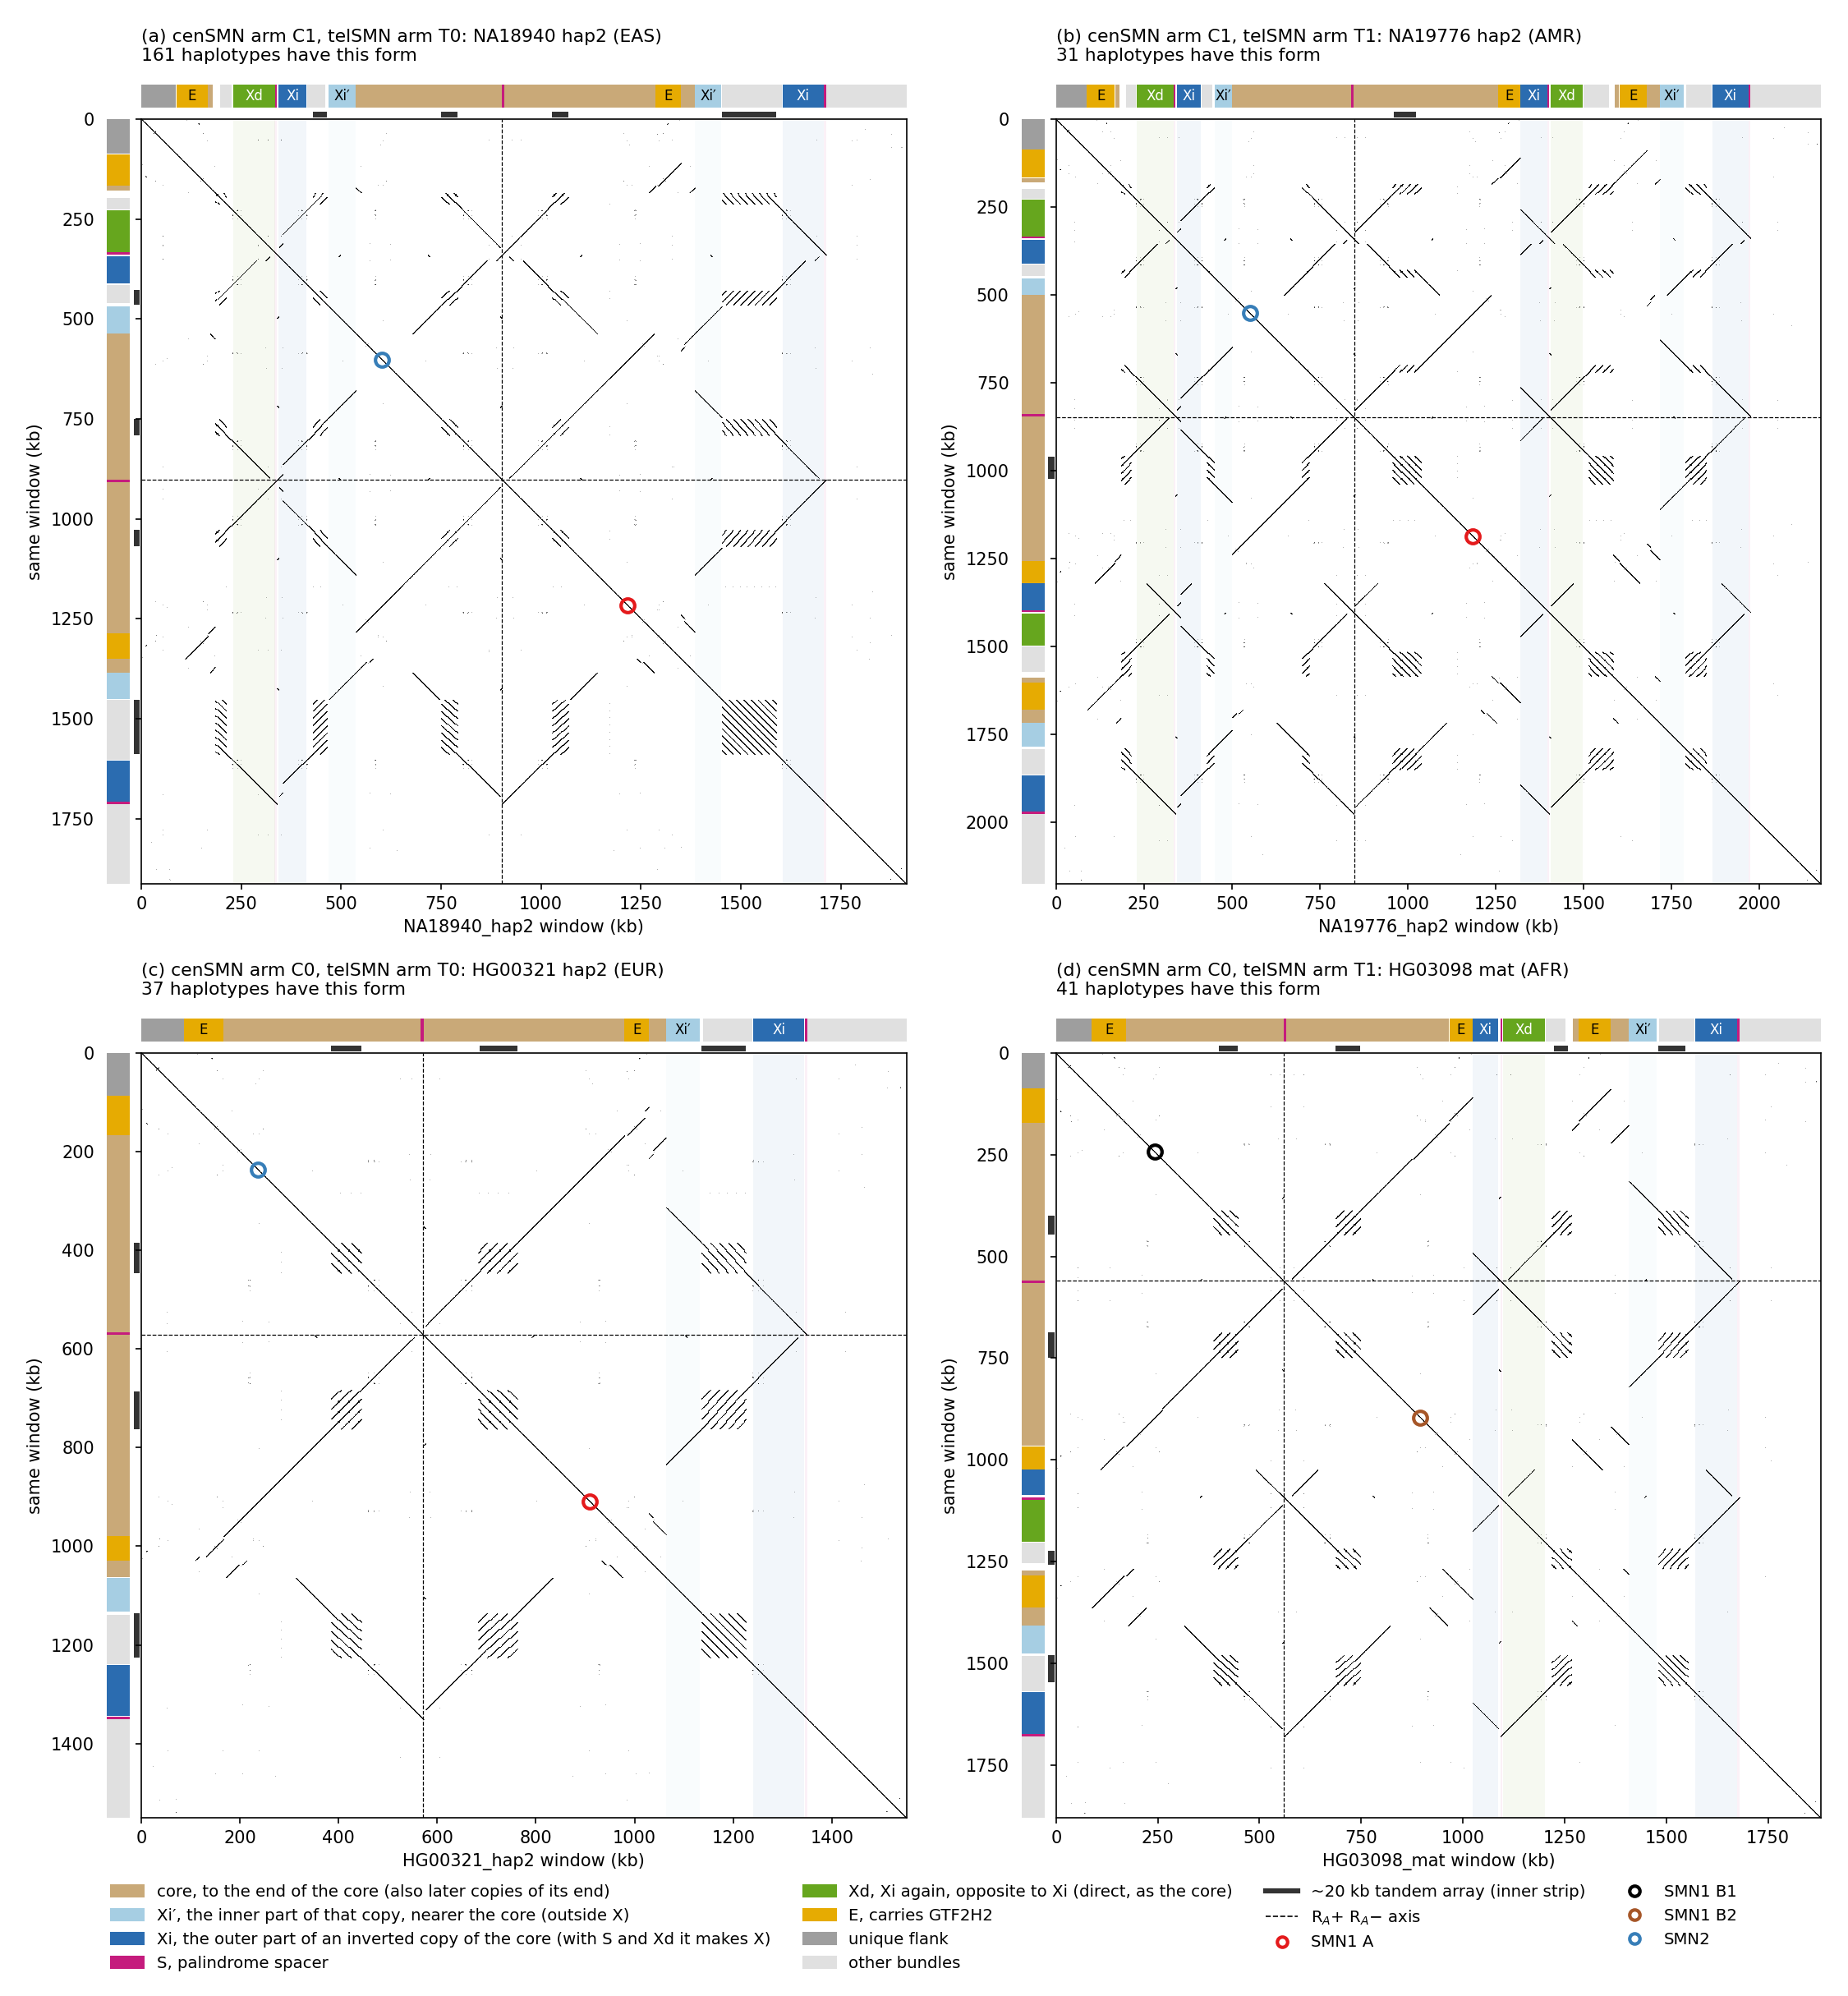
\includegraphics[width=\linewidth]{../figures/self_dotplots.png}
\caption{Self dot plots of one haplotype of each form: \textbf{a}, \dpAName{} (C1|T0; window \dpALen{} kb),
\textbf{b}, \dpBName{} (C1|T1; \dpBLen{} kb), \textbf{c}, \dpCName{} (C0|T0; \dpCLen{} kb) and \textbf{d},
\dpDName{} (C0|T1; \dpDLen{} kb). Dots: shimmers shared by two positions of the window (PANGEA's shimmer matcher, \texttt{get\_shmmr\_dots},
$w=\dpW$, $k=\dpK$, $r=\dpR$, minimum span \dpSpan). Strips along the axes: the arm elements (colors as in
Fig.~\ref{fig:palindrome}), S also at the axis, and the $\sim$20-kb tandem arrays (thin inner strip); shading marks Xi$'$, Xi,
S and Xd across the plot. Dashed lines: the axis of the \RU{A}+ \RU{A}$-$ pair. Circles: the SMN copies, on the main diagonal,
colored by gene and lineage. Drawn by \texttt{scripts/34\_dotplots\_graph.py}.}\label{fig:dotplots}
\end{figure}

\paragraph{Why X is called X (Fig.~\ref{fig:xcross}).} Drawn against itself, the cenSMN arm of a C1 haplotype shows
X directly: beyond the core, Xi and Xd form an inverted repeat, whose dots run across the main diagonal and
cross it at S (about \xcExS~kb from the axis in HG01099 mat). The element thus draws an X, and S, its center, is part of
it; the short break in the cross at S is the spacer itself, which has no partner. The C0 arm of the same donor has no
cross. Over all palindrome haplotypes, on each cenSMN arm \xcLo--\xcHi~kb from the axis we found where the off-diagonal
dots are centered (an inverted repeat centered at $c$ puts its dots on $x+y=2c$): on \xcTwenty{} of the \xcCOneS{} C1 arms
with an S in that stretch the strongest center lies within 20~kb of S, on \xcTen{} within 10~kb. The other \xcNoS{} C1 arms (\xcNoSNames) carry Xi and Xd with no S between
them and were not scored.

\begin{figure}[htbp]\centering
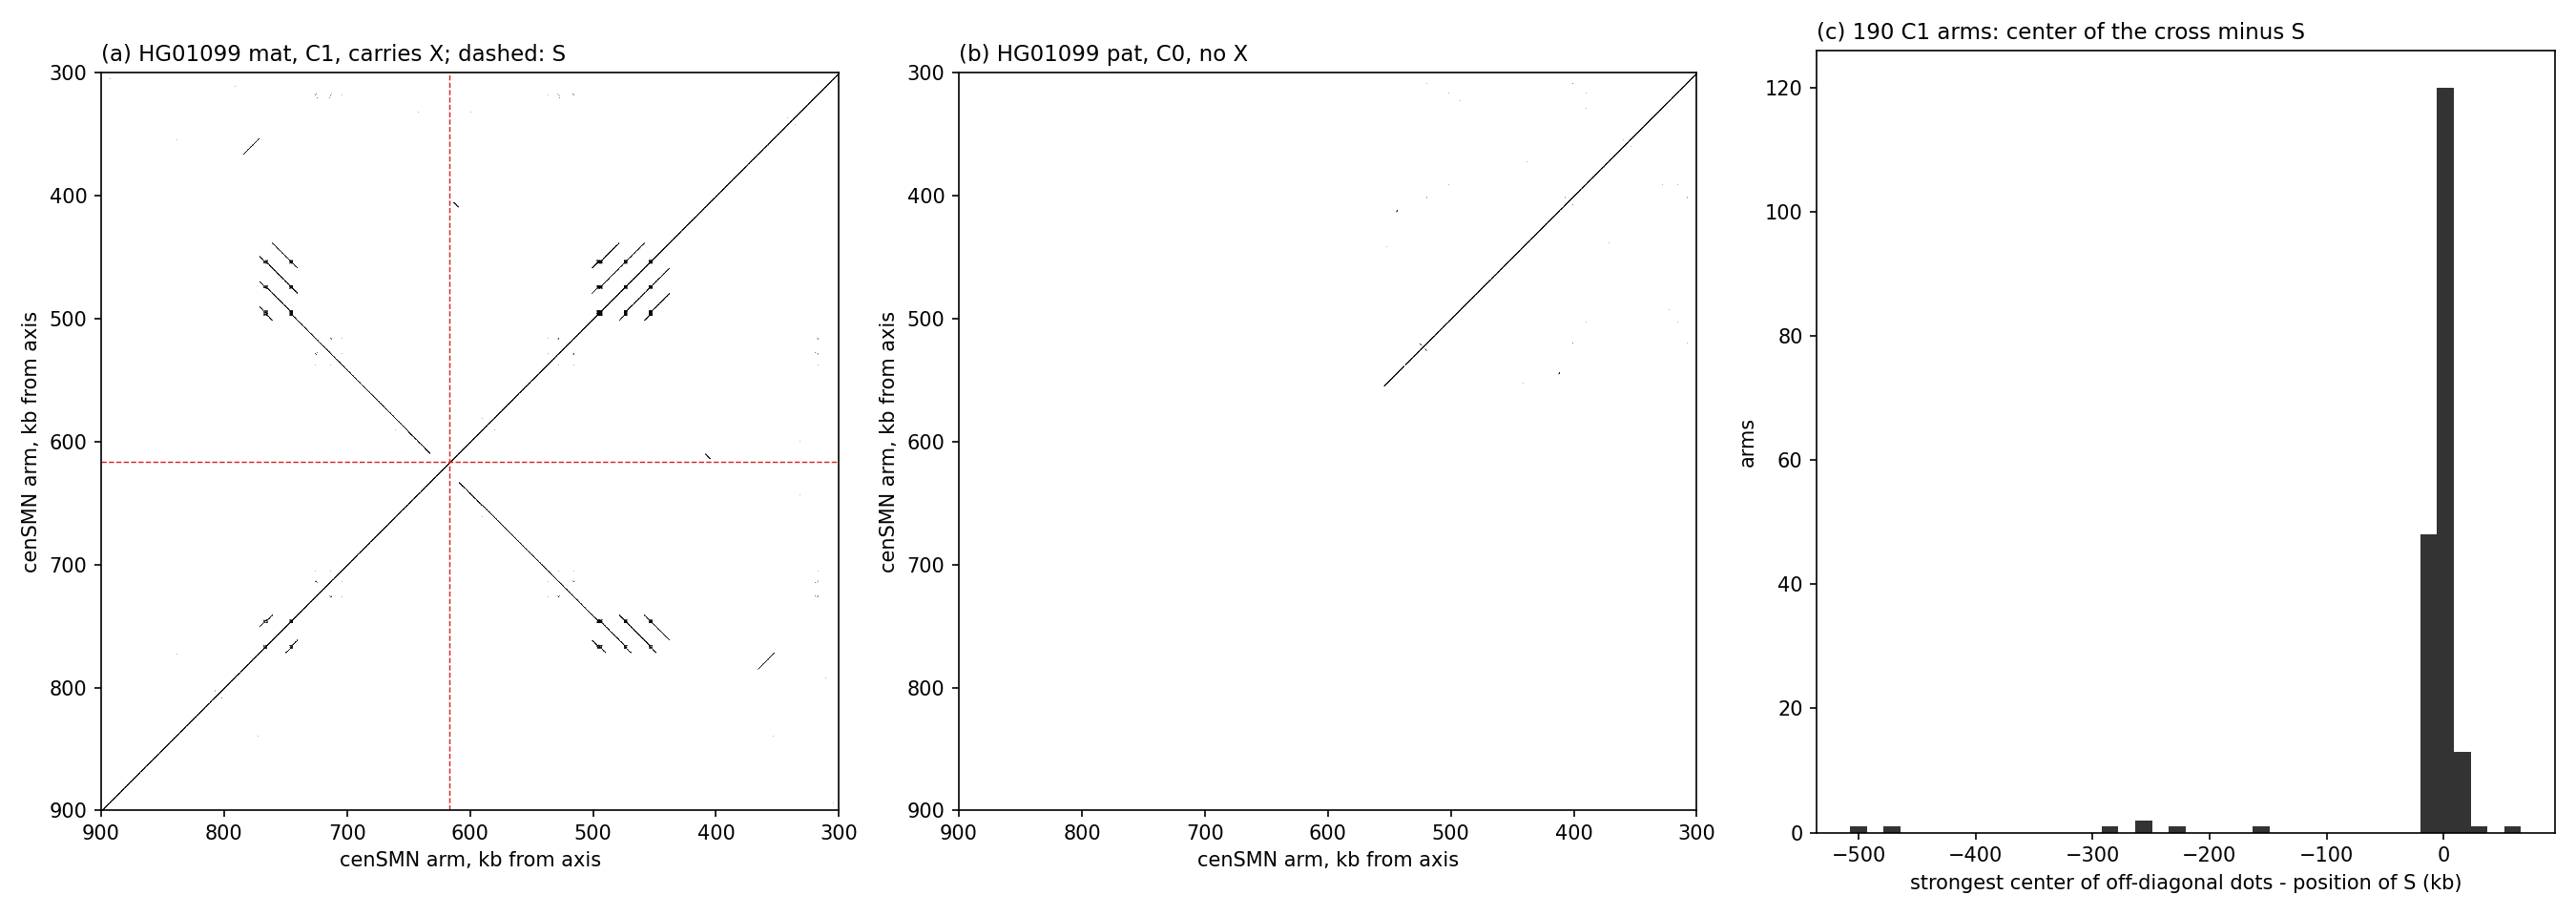
\includegraphics[width=\linewidth]{../figures/x_cross.png}
\caption{X in the sequence. \textbf{a}, \textbf{b}: self dot plots of the cenSMN arm, \xcLo--\xcHi~kb from the axis
(shimmers as Fig.~\ref{fig:dotplots}), of the two haplotypes of donor HG01099: \textbf{a}, mat, C1, whose X draws a
cross centered on S (dashed lines); \textbf{b}, pat, C0, no cross (its window ends \xcExCZeroArm~kb from the axis).
\textbf{c}: on the \xcCOneS{} C1 arms with an S in that stretch, the strongest center of the off-diagonal dots minus the
position of S. Drawn by \texttt{scripts/38\_x\_cross.py}.}\label{fig:xcross}
\end{figure}

\paragraph{SMN1 lineages on the arms.} Coloring the SMN1 copies of Fig.~\ref{fig:palindrome}c by lineage
(Section~\ref{sec:posstrand}) shows the same split as the copy positions. Of the \palSmnA{} lineage-A SMN1 copies on
the pair, \palARight{} sit on the right (\RU{A}$-$, telomeric) arm and \palALeft{} on the left. Of the \palSmnB{} lineage-B
copies, B1 sits on the left (\RU{A}+, centromeric) arm (\palBoneLeft, against \palBoneRight{} on the right) and B2 on the
right (\palBtwoRight, against \palBtwoLeft). The \elBB{} haplotypes with one B1 and one B2 copy all fall in the C0 forms
of panel c (\elBBTOne{} of them C0|T1). B copies sit somewhat further from the axis than A copies
(median \palBDist{} against \palADist{} kb; Mann--Whitney $p$~=~\palPDist{}), and the mirror is no less exact on
B-carrying haplotypes (median difference \palBMirror{} against \palOthMirror{} kb). These are descriptive: copies on one
haplotype are not independent, and B is almost only African.

\paragraph{Which copy sits on each arm (Table~\ref{tab:slots}).} Lefebvre et al.~\cite{lefebvre1995} named the two
SMN loci by position: telSMN, the telomeric copy (usually SMN1), and cenSMN, the centromeric copy (usually SMN2). On the
pair, the copy on the right (\RU{A}$-$, telomeric) arm is at the telSMN position and the copy on the left (\RU{A}+, centromeric) arm
at the cenSMN position. The right arm holds an SMN1 of lineage A in \slROthA{} of the \slROth{} haplotypes outside AFR. The left arm differs between the groups. Outside AFR it holds SMN2 in \slLOthTwo{} of
\slLOth{} (lineage A \slLOthA, lineage B \slLOthB). In AFR haplotypes it holds lineage B in \slLAfrB{} of \slLAfr{} (B1 \slLAfrBone, B2 \slLAfrBtwo),
SMN2 in \slLAfrTwo{} and lineage A in \slLAfrA: in this cohort's AFR haplotypes the commonest gene at the cenSMN
position is an SMN1 of sub-lineage B1. At the telSMN position of AFR haplotypes, B2 (\slRAfrBtwo) and A (\slRAfrA) are
about equally common, and B1 is rarer (\slRAfrBone).

This says where the copies sit today, not how they came to be there. Gene conversion
between the two loci is documented: van der Steege et al.~\cite{vandersteege1996} found hybrid genes of both kinds,
and Campbell et al.~\cite{campbell1997} report SMN1 replaced by its centromeric counterpart in milder SMA, the
opposite direction to B1. A conversion that turned a cenSMN copy into B1 would have
had to span the whole gene body, since B1 differs from SMN2 throughout it (Section~\ref{sec:grpdist}); these data do
not decide how B1 came to sit there.

\begin{table}[htbp]\small\centering
\caption{The copies and pieces on each arm of the \palPair{} pair haplotypes, by class (SMN1 split by lineage), for
AFR haplotypes and all others (``other'' includes the few ASL and unlabeled haplotypes). Column ``other'': the seven
$\Delta$7--8 copies and the one truncated piece, which shares its left arm with a counted copy (NA18959 hap1), so the
left arms hold one item more than the right (\slLOthItems{} items on the \slLOth{} left arms of the other groups). Hybrid: h12 and h21. Items: copies and pieces, not arms. From \texttt{27\_arm\_contents.py}
(\texttt{results/sv/arm\_slots.tsv}).}\label{tab:slots}
\begin{tabular}{@{}llrrrrrr@{}}\toprule
Arm & Haplotypes & SMN2 & SMN1 A & SMN1 B & Hybrid & Other & Items\\\midrule
\tabSlots
\bottomrule\end{tabular}
\end{table}

\paragraph{An arm holds one SMN copy.} \texttt{27\_arm\_contents.py} takes each of the \armN{} arms of the pair
haplotypes on its own. Every arm holds exactly one counted SMN copy (\armOneCopy{} of \armN; one left arm, NA18959 hap1,
also holds a truncated piece), inside the core on every arm (checked in step 28b); no element beyond the core holds an SMN copy.

% figure fig:palindrome is in the main text


\section{The structure differs between continental groups, most between AFR and the rest (Fig.~\ref{fig:ancestry})}\label{sec:ancestry}
\textbf{Question.} Does the large-scale structure of the region differ between the five continental groups? Unit: the
\anHaps{} resolved haplotypes of \anPeople{} people in AFR (\anNAfr), AMR (\anNAmr), EAS (\anNEas), EUR (\anNEur) and
SAS (\anNSas); ASL and unlabeled samples are left out. Every test permutes the group label of whole people (both
haplotypes together), so a person's two haplotypes are not counted as independent. Drawn and computed by
\texttt{09\_ancestry\_structure.py}.

\textbf{Answer: yes, and most of the difference is AFR against the rest, but not all of it.}
\begin{itemize}
\item \textbf{Arrangement types} (\anTypes{} types on five or more haplotypes, \anRare{} haplotypes of rarer types
pooled): $\chi^2=\anChi$, Cram\'er's $V=\anV$, permutation $p\le\anPArr$ (the floor that \anPerm{} permutations allow).
``2-~1+'' is \shTwoMOnePAfr\% of AFR haplotypes against \shTwoMOnePEur--\shTwoMOnePEas\% elsewhere (\shTwoMOnePEur\%
EUR, \shTwoMOnePSas\% SAS, \shTwoMOnePAmr\% AMR, \shTwoMOnePEas\% EAS); ``1-~1+'' is \shOneMOnePAfr\% in AFR against
at most \shOneMOnePSas\%; ``2+~1+'' (the GRCh38 type) is commonest in EAS (\shTwoPOnePEas\%); the $\Delta$7--8
type ``d2-~1+'' is seen only in AMR (\shDelTwoAmr\%) and EUR (\shDelTwoEur\%).
\item \textbf{Structural distance} (PANGEA's bundle distance): PERMANOVA over the five groups pseudo-$F=\anFAll$,
$R^2=\anRsqAll\%$, $p\le\anPAll$; over the four groups other than AFR, pseudo-$F=\anFNonAfr$, $R^2=\anRsqNonAfr\%$,
$p=\anPNonAfr$ (\anPermPA{} permutations each). Groups differ, but group explains under a tenth of the variation.
Median distance within a group is lowest in EAS (\anWEas) and highest in AFR (\anWAfr) and EUR (\anWEur), and AFR
haplotypes are about as far from each other as from any other group (between-group medians from \anAfrBetweenMin).
\item \textbf{Counts per haplotype} (group means; Kruskal--Wallis, people permuted):
the number of SMN copies per haplotype does \emph{not} differ (\anSmnAfr{} AFR to \anSmnAmr{} AMR, $p=\anPSmn$;
SERF1 $p=\anPSerf$), but what the units hold does: SMN1 by exon 7 is \anOneAfr{} in AFR against
\anOneEas--\anOneSas{} elsewhere, SMN2 \anTwoAfr{} in AFR against \anTwoEas{} in EAS ($p\le\anPOne$ and \anPTwo);
full-length NAIP follows SMN1 (\anNaipAfr{} AFR, \anNaipAmr--\anNaipEas{} elsewhere, $p=\anPNaip$); GTF2H2
(\anGtfEas{} EAS to \anGtfEur{} EUR, $p=\anPGtf$) and large repeat units (\anUnitsEas{} EAS to \anUnitsEur{} EUR,
$p=\anPUnits$) are lowest in EAS.
\end{itemize}
Read together: AFR haplotypes more often carry SMN1 where others carry SMN2 (the ``1-~1+'' type, B1 and B2 above) and are the
most varied; EAS haplotypes are the most alike; and the non-AFR groups also differ among themselves, though less.
The structural distance is PANGEA's score on the top bundles of each window, not the study's arrangement strings, and
the 1000 Genomes continental groups are coarse labels for the populations sampled.

\begin{figure}[htbp]
\centering
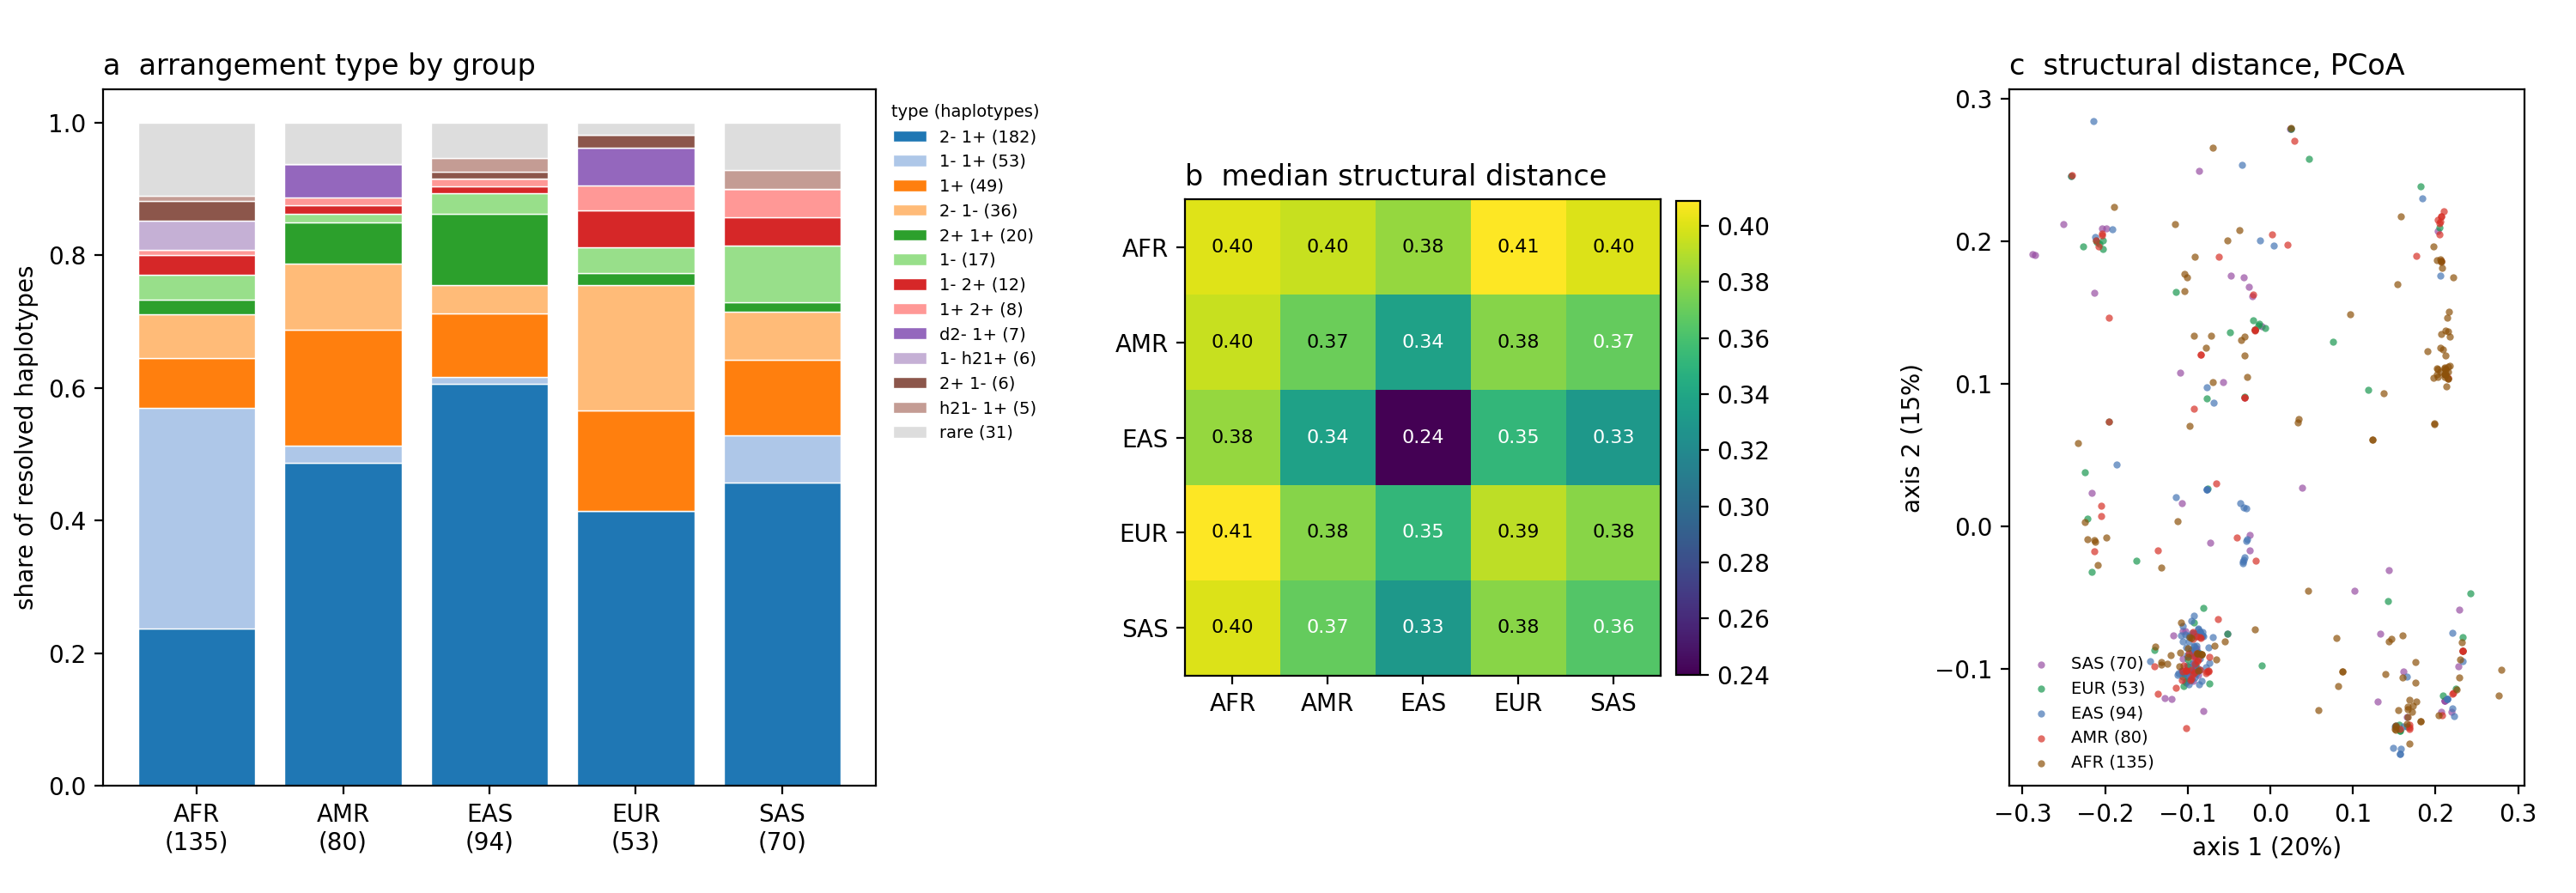
\includegraphics[width=\linewidth]{../figures/ancestry_structure.png}
\caption{Large-scale structure of the \anHaps{} resolved haplotypes by continental group. (a) Share of each
arrangement type (types on fewer than five haplotypes pooled as ``rare''; counts in the legend are over these
\anHaps{} haplotypes). (b) Median PANGEA structural distance within (diagonal) and between groups. (c) Principal
coordinates of the structural distance, one dot per haplotype, colored by group. Drawn by
\texttt{09\_ancestry\_structure.py}.}
\label{fig:ancestry}
\end{figure}

\section{Great-ape outgroups: one SMN copy per ape haplotype, and a proposed order of events (Fig.~\ref{fig:evo}, Table~\ref{tab:apes})}\label{sec:history}
\textbf{Question.} At the sites that set SMN1 lineage A, lineage B and SMN2 apart, which bases are ancestral, and
what order of events do they suggest? An outgroup is needed. Step 03 (\texttt{03\_outgroup\_alignment.sh}) adds the SMN gene body of chimpanzee, bonobo,
gorilla and orangutan (NCBI, the T2T primary assemblies of Table~\ref{tab:apes}) to the copy alignment as four more
rows, keeping its \nAlnCols{} columns (MAFFT \texttt{--add --keeplength}, which drops ape bases that would need new
columns);
\texttt{13b\_evolution\_sites.py} takes the gene-body columns where SMN1 (A and B together) and SMN2 are each at least
90\% fixed for different bases (\evS{} sites, ``paralog sites'') and those where A and B are (\evAB{} sites, ``A/B sites''),
and calls a base ancestral when at least three of the four apes carry it.

\textbf{How many SMN copies do the apes carry?} \texttt{14\_ape\_copies.py} and \texttt{15\_ape\_copies\_hap2.py}
search 5~Mb of each primary haplotype and 8~Mb (18~Mb for gorilla, whose chromosome is 7.7~Mb shorter) of each ape's
second haplotype for dense runs of SMN gene-body 25-mers. Each of the \apeHaps{} haplotypes holds exactly one copy
(\apeCopies{} copies), and a search at a lower density finds nothing outside these copies (on the second orangutan haplotype it returns \apeRelaxExtra{} further hit, inside that copy's own span; Table~\ref{tab:apes}). Across each whole genome, NCBI Gene lists
\apeGeneFull{} full-length SMN genes, one per ape at that locus, and \apeGeneShort{} other SMN-like records of
\apeShortMin--\apeShortMax{} bp elsewhere, which this study did not examine. Every ape copy carries SMN1's base at
c.840 (C) and c.*239 (G). Rochette et al.\ (abstract only)~\cite{rochette2001} reported 2--7 SMN copies per diploid
chimpanzee genome by quantitative PCR, and no SMN2 exon~7--8 bases in non-human primates. The one-copy finding in these
four individuals does not fit an SMN duplication that predates the human--chimpanzee split; whether the duplication is
human-specific or ape copy number varies between individuals is left open.

\textbf{Do the apes carry the large repeats? (Figs.~\ref{fig:apeself} and~\ref{fig:apehum}).} \texttt{35\_ape\_structure.py}
takes a 3-Mb stretch centered on each ape haplotype's SMN copy and plots it against itself with PANGEA's shimmer matcher
($w=\dpW$, $k=\dpK$, $r=\dpR$, the settings of the human dot plots), and against one human window, HG01099 mat
(Fig.~\ref{fig:locus}a), whose arm elements are known. None of the ape stretches shows a long off-diagonal line: they have
\apFarLo--\apFarHi{} dots per Mb more than 50~kb off the diagonal, the human window \apFarHum{} per Mb, and the ape dots off the diagonal
form short columns, as interspersed repeats do (Fig.~\ref{fig:apeself}). Against the human window (Fig.~\ref{fig:apehum}),
chimpanzee, bonobo and gorilla each place both human core arms on one ape stretch: \apShareLo--\apShareHi\% of each arm's
matches fall in the same \apWin-kb ape stretch, in the same order from the human axis (Spearman $\rho>0.9$ on each arm), so
the human plot folds into a V at the axis; Xi and Xd fold onto the same ape stretch again. In orangutan the matches are
sparse and at most \apOruShare\% fall in one stretch. S matches chimpanzee and bonobo at \apSPanLo--\apSPanHi{} times the
rate of the human window's unique flank, and gorilla and orangutan at no more than \apSOtherHi{} times it
(\path{results/sv/ape_fold.tsv}). One copy of the human core per ape haplotype, with both human arms on it, fits a
palindrome that formed in the human lineage after the split from these apes; the ape stretches are one assembly per
species and one human haplotype is the reference, and the absence of S in gorilla and orangutan is within 1.5~Mb of
the copy only.

\begin{figure}[htbp]\centering
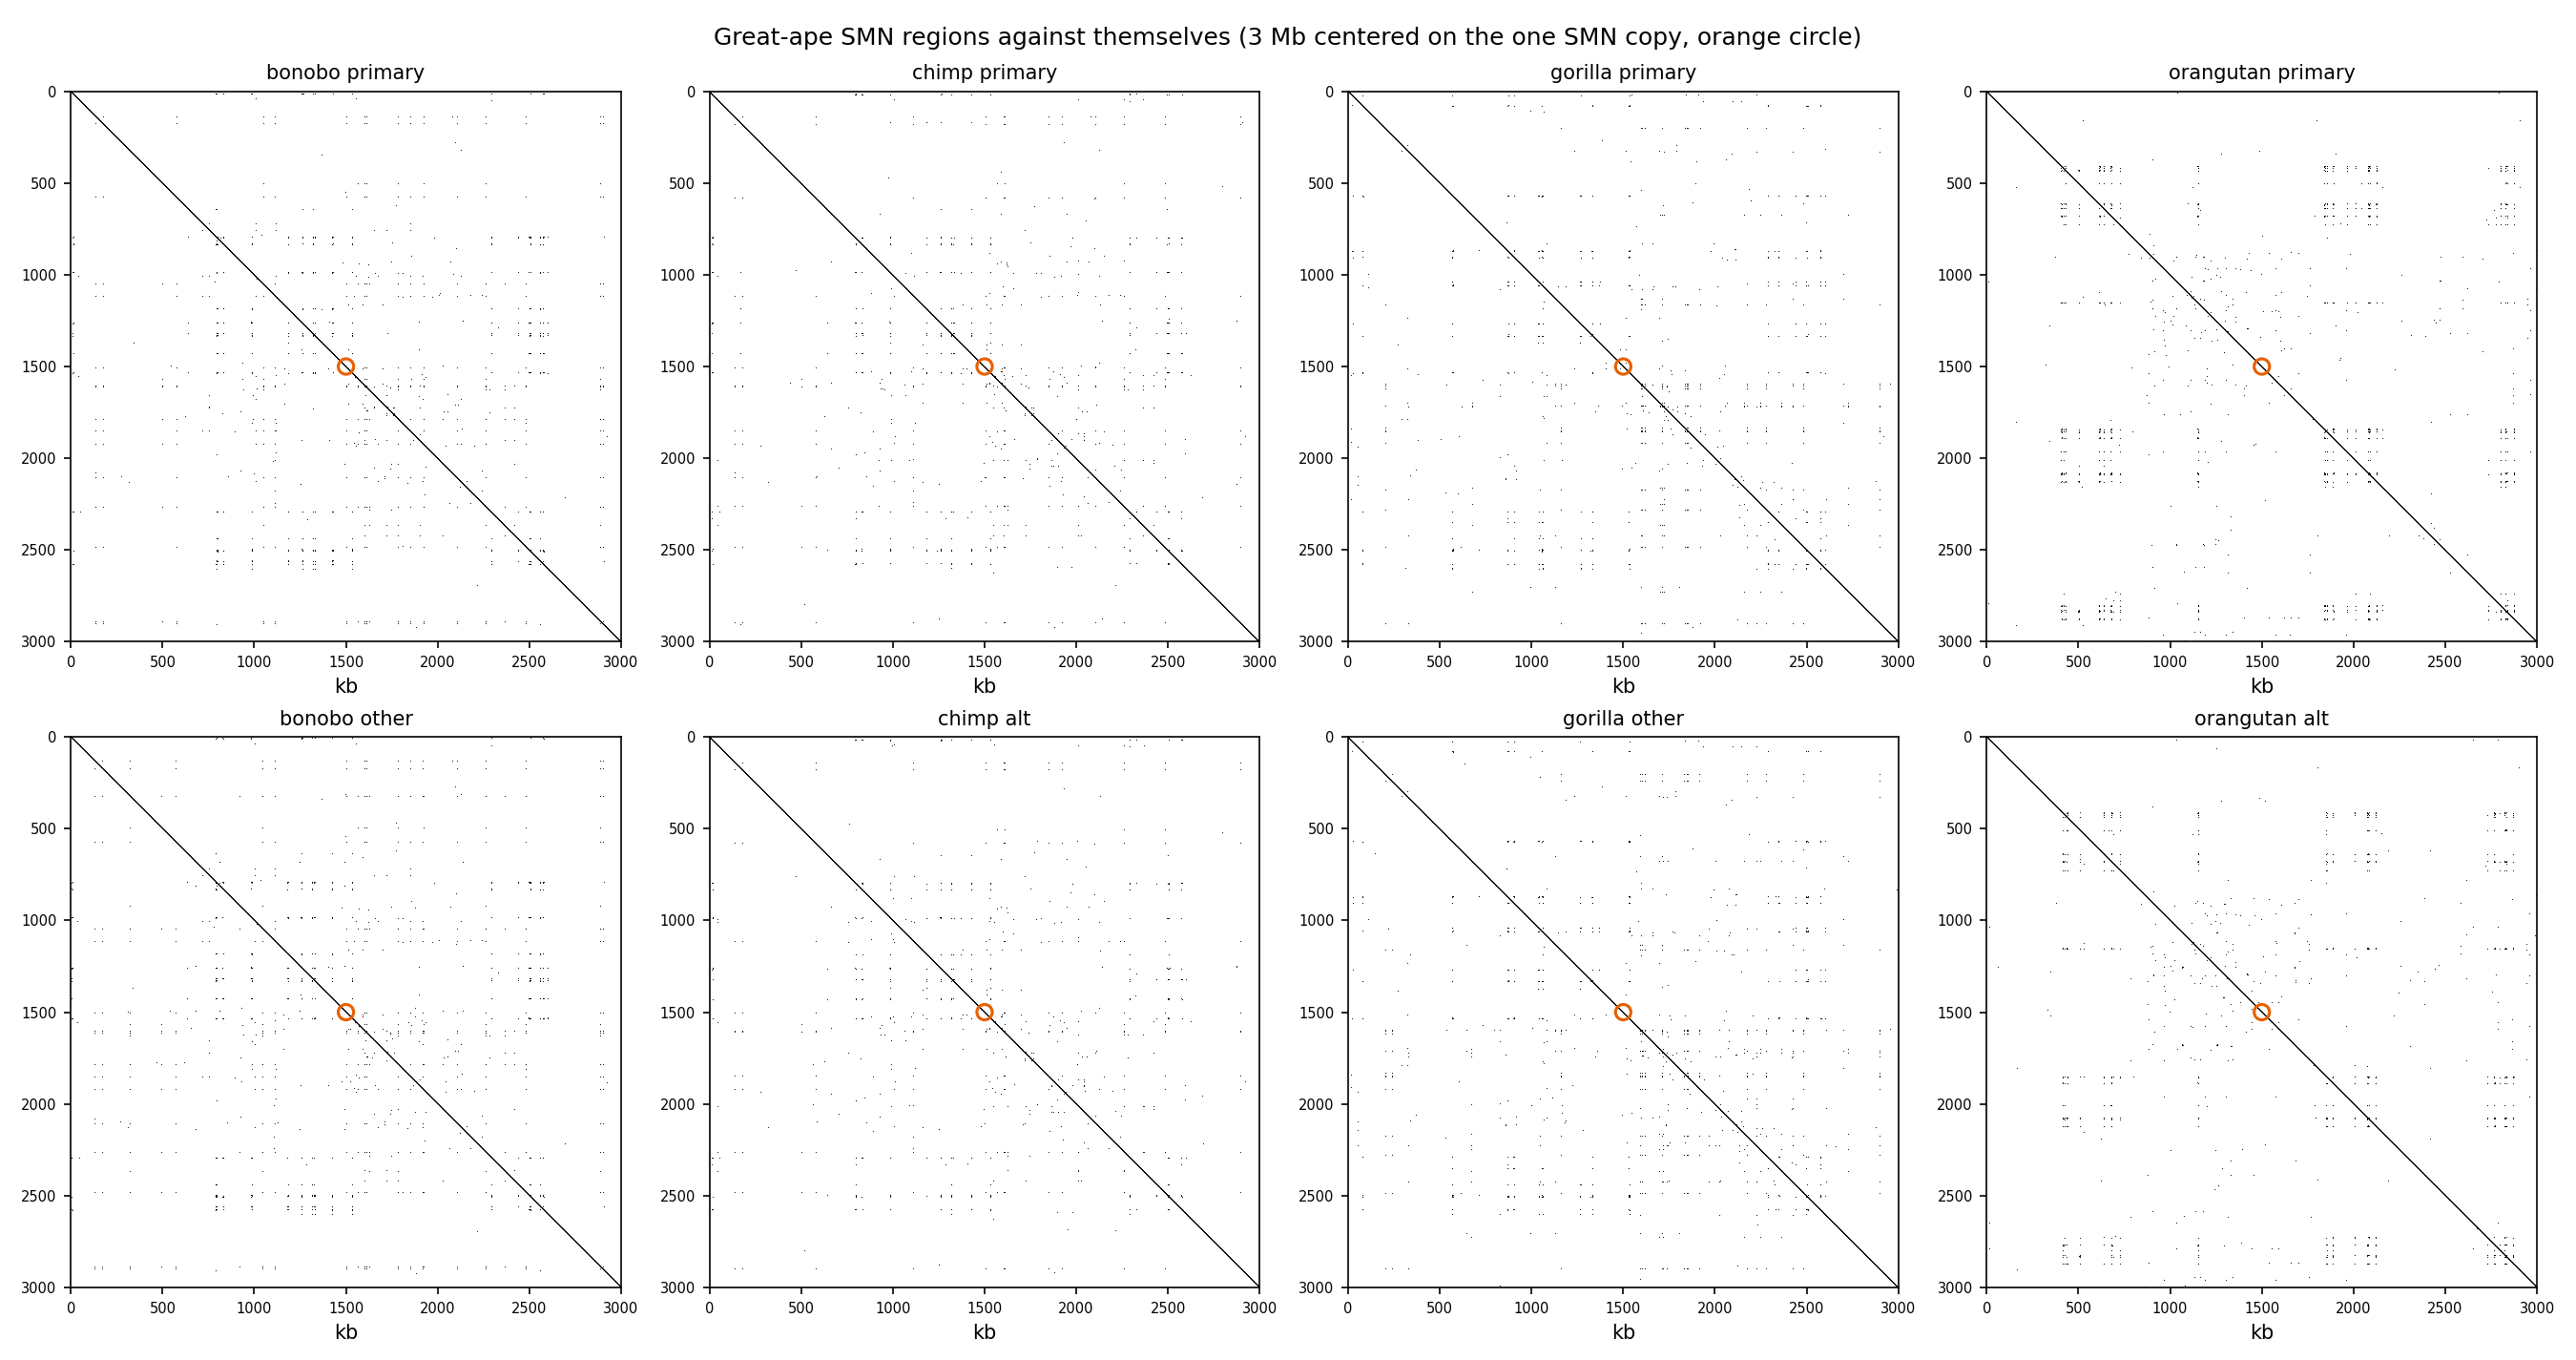
\includegraphics[width=\linewidth]{../figures/ape_self_dotplots.png}
\caption{Each great-ape haplotype's SMN region against itself: 3~Mb centered on its one SMN copy (orange circle), shimmer
matches as dots ($w=\dpW$, $k=\dpK$, $r=\dpR$). Only the main diagonal and short columns of interspersed repeats appear; no
long inverted or direct repeat. ``Other'' and ``alt'' are each ape's second haplotype assembly.}\label{fig:apeself}
\end{figure}

\begin{figure}[htbp]\centering
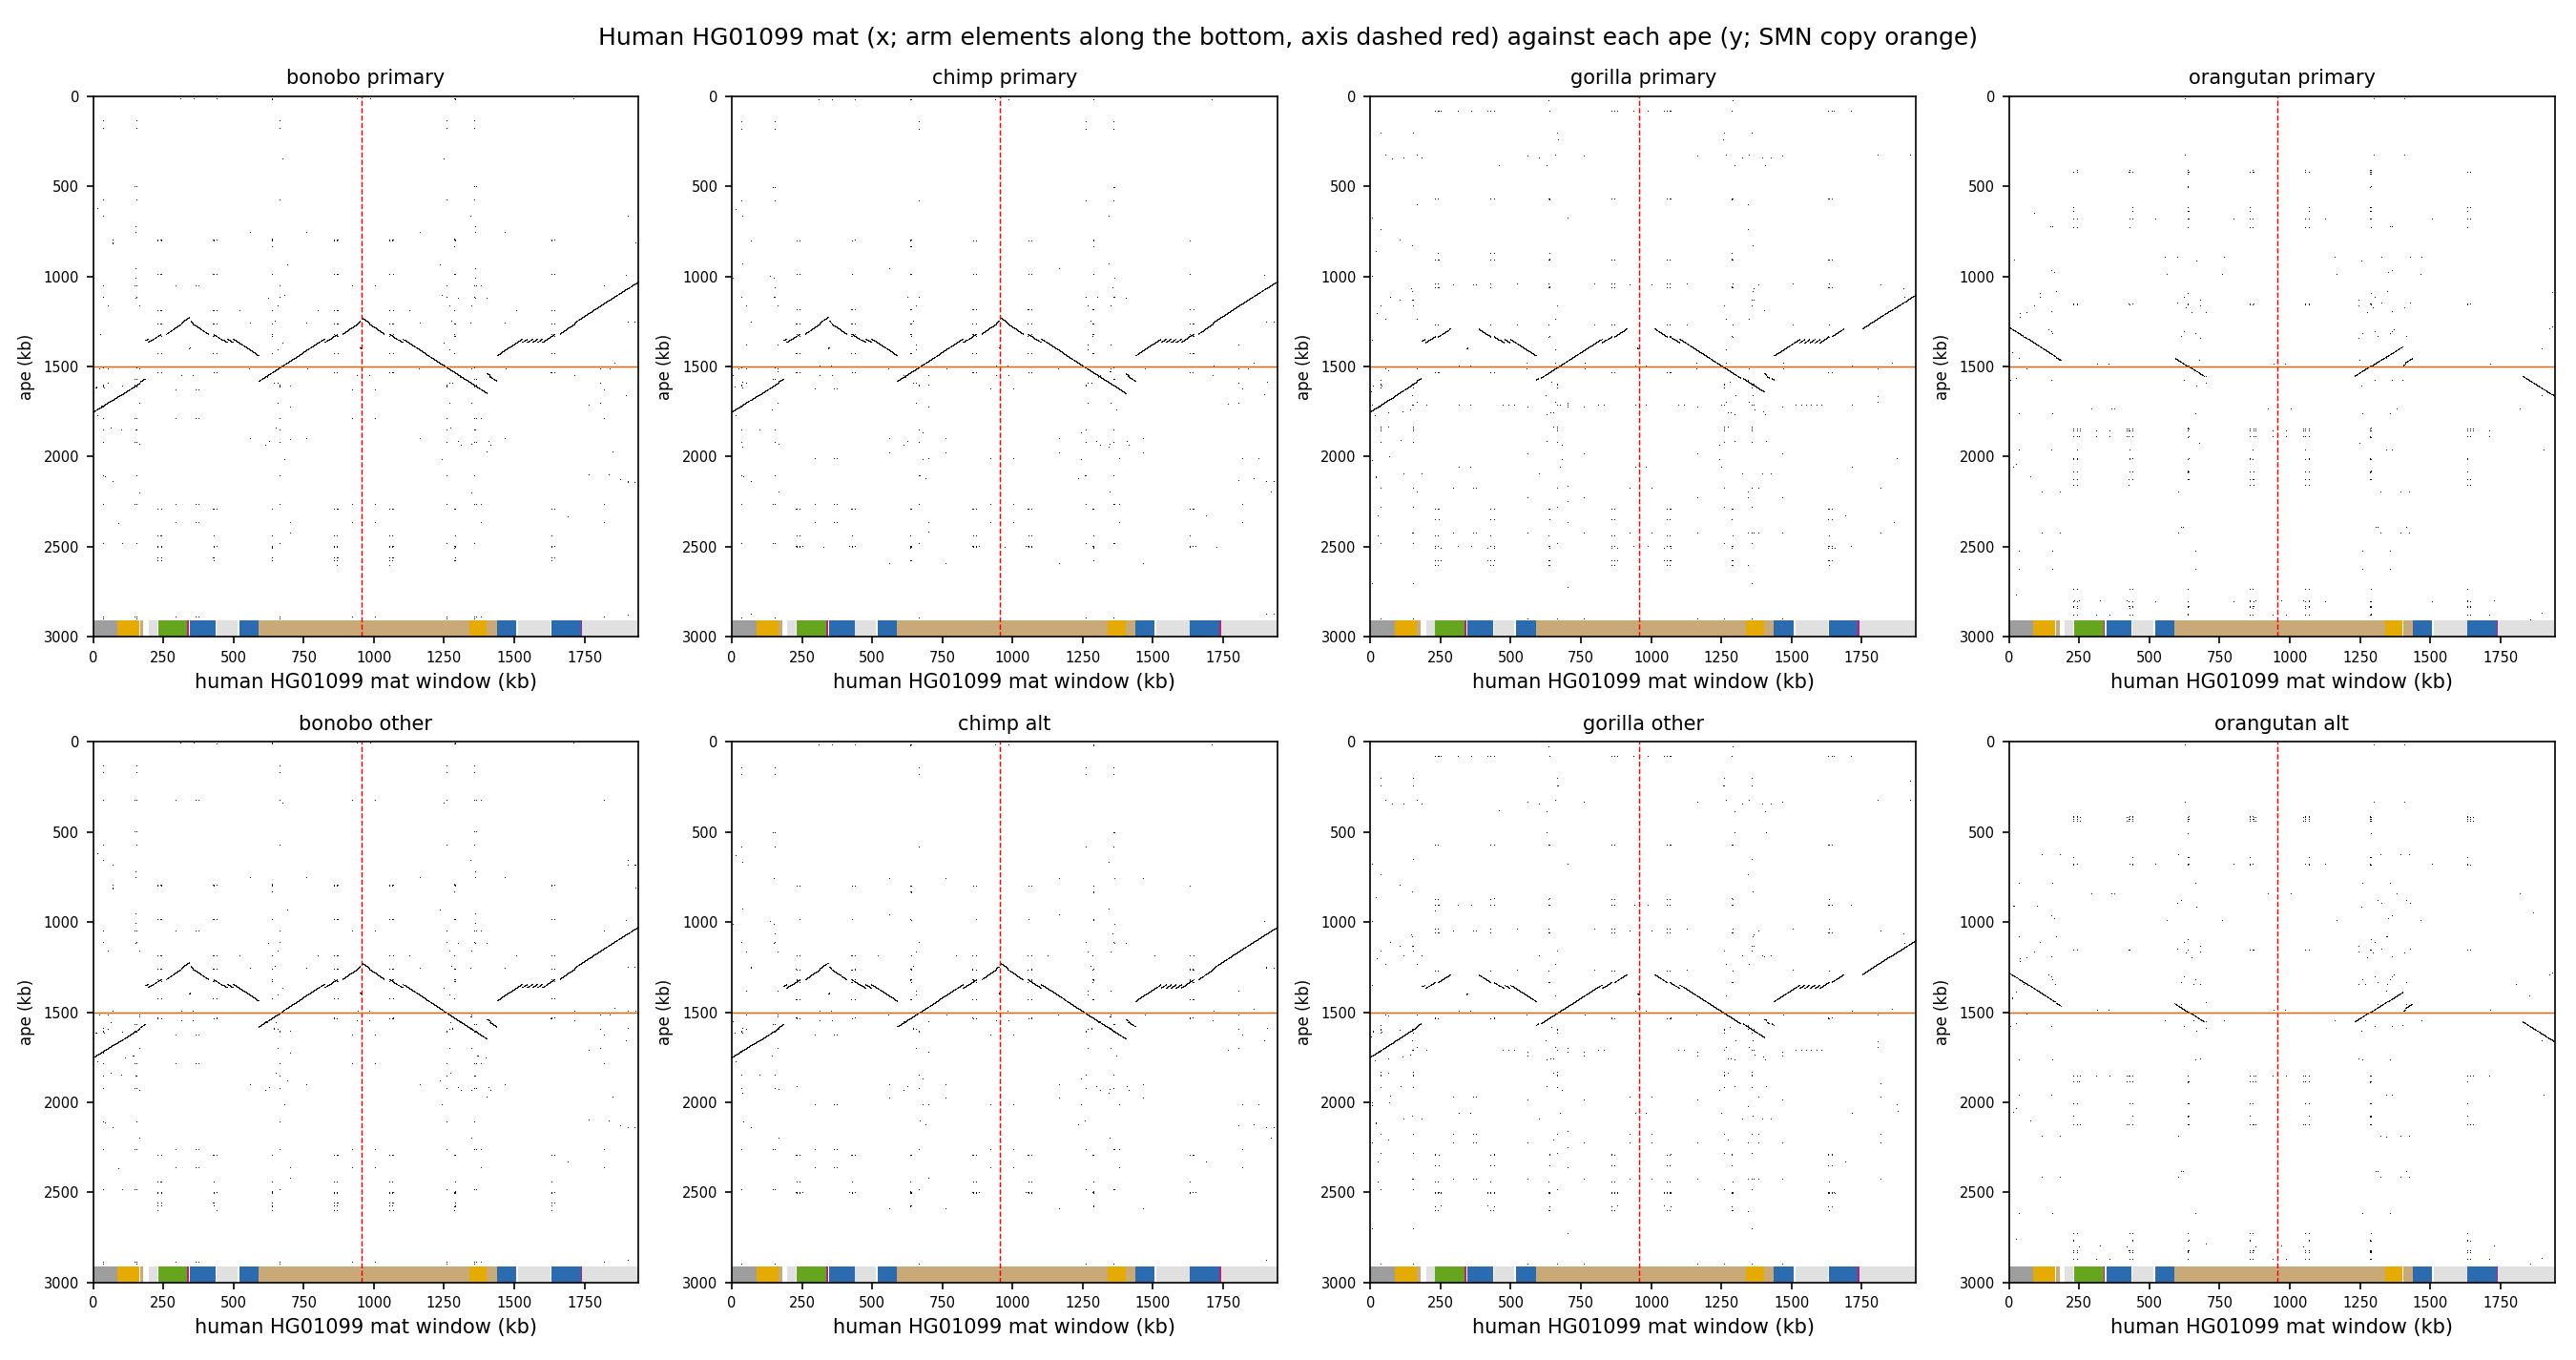
\includegraphics[width=\linewidth]{../figures/ape_vs_human.png}
\caption{The human window HG01099 mat (x; its arm elements along the bottom, colors as in Fig.~\ref{fig:palindrome};
axis of the \RU{A}+ \RU{A}$-$ pair dashed red) against each ape stretch (y; the ape SMN copy, orange line). In chimpanzee, bonobo and
gorilla both human arms run onto the same ape stretch, folding into a V at the human axis; in orangutan only short pieces
match.}\label{fig:apehum}
\end{figure}

\begin{table}[htbp]\small\centering
\caption{The SMN copy found in each great-ape haplotype searched: assembly sequence, start, strand, the bases at
c.840 and c.*239, and the base counts at the \evS{} paralog sites (SMN1/SMN2) and the \evAB{} A/B sites (A/B), each copy
aligned pair-wise to GRCh38 SMN1. Pair-wise counts can differ from the counts in the text, which use each ape's base read from its raw sequence (step~13c; see below); those read-checked counts are the last two columns, for the primary assemblies (unresolved sites counted in neither). ``Second'' is the species' other haplotype assembly. Each haplotype holds one whole SMN copy. The lower-density search finds nothing outside these copies; on the second orangutan haplotype it returns \apeRelaxExtra{} further hit, over \apeOrangPartCov{} of the gene body, which lies inside that copy's own span and on the opposite strand, and is not a second copy. From \texttt{results/sv/ape\_copies.tsv} and \texttt{results/sv/ape\_copies\_hap2.tsv}.}\label{tab:apes}
\footnotesize\setlength{\tabcolsep}{4pt}\begin{tabular}{@{}lllrlccrrrr@{}}\toprule
Ape & Haplotype & Sequence & Start & Strand & c.840 & c.*239 & paralog & A/B & paralog, read & A/B, read\\\midrule
\tabApes
\bottomrule\end{tabular}
\end{table}

\textbf{What the sites say.}
\begin{itemize}
\item \textbf{SMN1 against SMN2.} All \evS{} paralog sites lie in chr5:\evSfrom--\evSto{} (\evSspanKb{} kb, intron~6 to
exon~8). They are \bzMatch{} of the \bzPsvN{} paralogous sequence variants (PSVs) in Fig.~4 of Berzal-Serrano et al.~\cite{berzal2026}: \bzExact{} carry the same c.\ name there, and \bzOff{} in intron~6 sit \bzOffBp{} bases from theirs, with the same spacing and bases. Their PSVs \bzUnmatched{} are not among our paralog sites. The apes carry SMN1's base at \evSancOne{} (c.840 and c.*239 among them, so SMN2's bases there are new) and
SMN2's at \evSancTwo{} (unresolved \evSunres). A and B both carry SMN1's base at every paralog site, and share the newer
SMN1 base at \evSsharedAB: in this stretch A groups with B.
\item \textbf{A against B.} The \evAB{} A/B sites lie in chr5:\evABfrom--\evABto, between exon~1 (5$'$ untranslated part) and intron~2, upstream of that
stretch. The apes carry B's base at \evABancB{} and A's at \evABancA{} (unresolved \evABunres). Per ape, A's base at
\evABAChimp{} (chimpanzee), \evABABonobo{} (bonobo), \evABAGorilla{} (gorilla) and \evABAOrang{} (orangutan) sites. These ape bases are read from each ape's raw primary-assembly sequence, not from the multiple alignment: the 101-bp GRCh38 context of each site is aligned locally to the ape's region and the read kept when it covers the site at identity $\geq$0.85 with no gap within 3 bases (step~13c; \rdAcc{} of \rdN{} ape--site reads kept; a read not kept leaves the alignment's base only where the two agree). The kept reads differ from the multiple alignment in \rdMsaDiffN{} cases, \rdMsaDiff; the alignment had placed those orangutan bases wrongly. The weakest kept read is orangutan at chr5:\rdWeakSite: its best local match scores \rdWeakScore{} against \rdWeakSecond{} for the next best (\rdWeakOthLo--\rdWeakOthHi{} for the other three apes there). Set aside, the site would still carry B's base in chimpanzee, bonobo and gorilla; a second assembly per species would settle it. At \rdUnresSite, the last base of a run of 14 T before 5 G in GRCh38, no ape aligns cleanly across the site, so it is unresolved in all four (the alignment had given G, or a gap in orangutan). Pair-wise typing (Table~\ref{tab:apes}) differs from the read sequence in \apeDiffN{} site--ape cases (\apeDiffSites); the primary orangutan copy's pair-wise match is the weakest (21-mer share \apeOrangKmer, against \apeOtherKmerLo--\apeOtherKmerHi{} for the other apes).
\item \textbf{A with SMN2 upstream.} SMN2 carries A's base at \evABtwoEqA{} of the \evAB{} A/B sites. At \evABtwoEqAanc{}
of them A's base is the ape base, which groups nothing; at the other \evABsharedATwo, where B keeps the ape base, A and
SMN2 share the newer base. Upstream, A groups with SMN2, as the maximum-likelihood tree does over the whole gene body.
\end{itemize}

\textbf{A proposed order (a hypothesis, Fig.~\ref{fig:evo}).} (1) The human and ape lineages split, with one SMN copy
in the ancestor as far as these assemblies show; (2) the single ape copy is a mix at the paralog sites (SMN2's base at
\evTwoBaseChimp, \evTwoBaseBonobo, \evTwoBaseGorilla{} and \evTwoBaseOrang{} of them in chimpanzee, bonobo, gorilla
and orangutan); (3) the human copies divide into lineage B's side and a side holding A and SMN2, which share newer bases
upstream; (4) SMN2 gains its defining bases in the \evSspanKb-kb stretch, where A and B keep or share SMN1 bases; (5)
conversion and unequal crossing-over go on, giving the hybrids. The evidence conflicts by region: \evSsharedAB{} newer
bases group A with B in the intron~6--exon~8 stretch, and \evABsharedATwo{} group A with SMN2 upstream. Gene conversion
between copies, which Suzuki et al.~\cite{suzuki2026} report as putatively biased and one-way around
SMN, would give such a regional mix under other orders too. The evidence rests on \evS{} and \evAB{} sites and one copy
per ape haplotype; the maximum-likelihood tree adds the cautions of Section~\ref{m:hist}.

% figure fig:evo is in the main text



\section{The finer bundle scale: the same comparisons on a finer decomposition}\label{sec:fine}
Beside the study's bundle decomposition (step 00), a finer one, with more and shorter bundles, is run as a check (Table~\ref{tab:decomp}). Its repeat-unit families are written \RUf{A}, \RUf{B}, \dots; their letters are assigned separately from the study's \RU{A}, \RU{B}, \dots\ and do not correspond to them. The coarse
decomposition captures the large structure with fewer, longer bundles; the finer one keeps more detail. Both are run on
the same \wfN{} windows, and the structural distances they give have rank correlation \tsStructRho{} over all pairs of
windows. The main text uses the coarse one. This section reports what the finer one gives: the association tests,
recomputed on its distance (steps 01b and 28i), and the bands, arm forms, repeat-unit families and copy positions on it (step 37,
\path{results/sv/fine/}). Its set of
pair haplotypes (\fafTOneAll{} with a T1 and \fafTZeroAll{} with a T0 arm) differs slightly from the coarse one, so its counts are of its own set.

\begin{table}[htbp]\small\centering
\caption{The two bundle decompositions: every setting of \texttt{pangea cohort bundle decomp} (given on the command
line, or PANGEA's default where marked), and the result. Both are run on all windows together; \texttt{repeat-units}
is run on each at its default settings and \texttt{dist} with \texttt{--top-n \setTopN}. From
\texttt{results/sv/decomp\_params.tsv} (step 28i), the commands read from each BED file's header and the defaults from
\texttt{decomp --help}.}\label{tab:decomp}
\begin{tabular}{@{}lrr@{}}\toprule
Setting & Coarse (main text) & Finer (this section)\\\midrule
\tabDecomp
\bottomrule\end{tabular}
\end{table}

\paragraph{The association between structure and sequence (Table~\ref{tab:twoscales}).} With the same haplotypes, the same
sequence distances and the same shuffles, the Mantel correlation is a little higher on the finer decomposition in
\tsHigherFine{} of the \tsTests{} Mantel tests, the cophenetic correlation too (\tsCophC{} against \tsCophF), and every Mantel test has $p=$\,\mantelP{} at both scales. The difference is largest
within C0 arms (\tsCZeroC{} against \tsCZeroF) and absent within T1 arms (\tsTOneC{} against \tsTOneF). Finer
bundles may hold more of the link to the bases, but how much depends on the arm type: this is an observation, not a
rule. The two correlations of a test come from the same haplotypes, and no test of their difference was made.

\begin{table}[htbp]\small\centering
\caption{Mantel correlation (Spearman) between structural and SMN sequence distance at the two bundle scales, and the
cophenetic correlation of the structure tree (UPGMA) with the gene-body maximum-likelihood tree (Section~\ref{sec:cophen}). Arm-type rows use the SMN1 copies of haplotypes with that arm type, so the
type itself cannot make the correlation. Every Mantel $p\le$\,\mantelP{} (\nPerm{} shuffles, one seed per test shared
by both scales). From \texttt{results/sv/two\_scales.tsv} (step 28i).}\label{tab:twoscales}
\begin{tabular}{@{}lrrr@{}}\toprule
Test & Haplotypes & Coarse & Finer\\\midrule
\tabTwoScales
\bottomrule\end{tabular}
\end{table}

\paragraph{Bands (Table~\ref{tab:twoscalebands}).} With the same structure cut (\setK{} clusters) and the same
sequence clusters, the finer decomposition gives four bands. Three are the coarse bands again: the B1\,+\,B2 band
(all \fbABinCoarse{} of its \fbABn{} haplotypes are in the coarse one), the S1-2 band (\fbTwoinCoarse{} of its
\fbTwon{}, and all of the coarse one's) and the bulk (\fbBulkinCoarse{} of its \fbBulkn). The fourth is an S1-3 band of
\fbThreen{} haplotypes (\fbThreeexp{} expected, $p=\fbThreep$), mostly ``2-~1+'' and ``1+'', each with one forward
SMN1 copy of haplogroup S1-3. On the coarse decomposition these haplotypes fall in the bulk's structure cluster
(\fbThreeToBulk) and the B1\,+\,B2 band's (\fbThreeToAB), and form no band.

\begin{table}[htbp]\small\centering
\caption{The bands at the two bundle scales (sequence side from the supported maximum-likelihood clades in both).
$n$, haplotypes; exp., expected by chance; $p$, Bonferroni-corrected hypergeometric. Coarse: \texttt{results/sv/ml\_vs\_upgma\_bands.tsv};
finer: \texttt{results/sv/fine/ml\_vs\_upgma\_bands.tsv}.}\label{tab:twoscalebands}
\begin{tabular}{@{}lrrrrrr@{}}\toprule
& \multicolumn{3}{c}{Coarse} & \multicolumn{3}{c}{Finer}\\\cmidrule(lr){2-4}\cmidrule(lr){5-7}
Band & $n$ & exp. & $p$ & $n$ & exp. & $p$\\\midrule
Bulk & \cbBulkn & \cbBulkexp & $\cbBulkp$ & \fbBulkn & \fbBulkexp & $\fbBulkp$\\
S1-2 band & \cbTwon & \cbTwoexp & $\cbTwop$ & \fbTwon & \fbTwoexp & $\fbTwop$\\
S1-3 band & -- & -- & -- & \fbThreen & \fbThreeexp & $\fbThreep$\\
B1\,+\,B2 band & \cbABn & \cbABexp & $\cbABp$ & \fbABn & \fbABexp & $\fbABp$\\\bottomrule
\end{tabular}
\end{table}

\paragraph{The structure clusters against arm form.} On the finer decomposition the S1-3 and B1\,+\,B2 bands shared one
structure cluster (\fafMixClu{} haplotypes), and the clusters split by the telSMN arm type rather than the cenSMN one:
all \fafMixPair{} haplotypes with the pair in that cluster had a T1 arm (\fafMixCOne{} C1|T1, \fafMixCZero{} C0|T1),
and none of the \fafBulkPair{} in the bulk's cluster (\fafBulkClu{} haplotypes; Fisher $p=$\,\fafP). The S1-3 band held
\fafThreePair{} haplotypes with the pair, all C1|T1, and \fafThreeNoPair{} without it; the B1\,+\,B2 band's
\fafABCZTOne{} were all C0|T1. So the cenSMN arm separates the two large clusters on the coarse decomposition, and the
telSMN arm on the finer one; which arm the structural distance weighs most depends on the bundle scale.

\paragraph{Family~\RUf{G} and the S1-3 band.} On the finer decomposition a repeat-unit family~\RUf{G}, a unit of median \sGkb{} kb,
was on all \sBandG{} S1-3 band haplotypes and on \sCenG{} of the \sCen{} in the bulk; restricted to ``2-~1+''
haplotypes, \sBandTwoOneG{} of \sBandTwoOneN{} against \sCenTwoOneG{} of \sCenTwoOneN{}.
Family~\RUf{C} was on \sBandC{} of \sBand{} against \sCenC{} of \sCen, and family~\RUf{D} on \sBandD{} against \sCenD. Across the
\sHaps{} resolved haplotypes with an SMN1 copy, \sGandT{} of the \sTall{} carrying an S1-3 copy had an \RUf{G} unit, but so
did \sGnotT{} others, so \RUf{G} was not specific to S1-3. Among \RUf{G} carriers, the S1-3 haplotypes (\sGThreeC{} of \sGThreen{}
with \RUf{C}) and the S1-2 haplotypes (\sGTwoC{} of \sGTwon{}) shared the \RUf{C} units and mostly lacked \RUf{D}, while the
S1-8/S1-9/S1-6 haplotypes carried \RUf{D} (\sGEightD{} of \sGEightn) and rarely \RUf{C} (\sGEightC). In elements, \RUf{G} was Xi with S
(\ffeGcombo{} of its \ffeGocc{} occurrences on haplotypes with the pair), on \fafGTOne{} of the \fafTOneAll{}
haplotypes with a T1 arm and \fafGTZero{} of the \fafTZeroAll{} with T0: the T1 arm under another name. On the coarse decomposition the family that
marks the T1 arm is \RU{\afSigFam} (Section~\ref{sec:bands}).

\paragraph{Why the copy sits further out on C0 and T1 arms.} On the finer decomposition the stretch of the core between
bundles 40 and 16 holds the inner $\sim$20-kb array. It was a median \fcpArrCZero~kb on the \fcpNCZero{} C0 arms
against \fcpArrCOne~kb on the \fcpNCOne{} C1 arms (the arms on which both bundles were found), one unit more, while the rest of the axis-to-copy distance was the
same (\fcpRestCZero{} and \fcpRestCOne~kb): the C0 copy's extra \fcpDiffCopycen~kb was the stretch
(\fcpDiffArrcen~kb). On the telSMN arm, T1 against T0, the stretch was \fcpArrTOne{} against \fcpArrTZero~kb and the
rest \fcpRestTOne{} against \fcpRestTZero~kb. The stretch took few lengths, \fcpModes~kb, one array unit apart
(Spearman correlation of copy distance with the stretch \fcpRhocen{} on the cenSMN and \fcpRhotel{} on the telSMN
arm; \path{results/sv/fine/copy_position.json}).

\paragraph{Why the finer unit call split \RUf{A} into long and short.} On the finer decomposition PANGEA's \texttt{repeat-units} called an \RUf{A} unit long (\elUnitLong~kb or more, the same cut as in Section~\ref{sec:palindrome}) on some arms and short on others, and the two did not follow the arm elements. HG03816 pat and HG01099 mat (the top two windows of Fig.~\ref{fig:pgraph}) carry the same arm elements in the same order, yet with the finer bundles PANGEA called a short \RUf{A}+ unit with \RUf{B}$-$
beyond it in the first and one long \RUf{A}+ unit in the second. Only the tandem arrays differ: the outer array of the telSMN arm
has \grPatTel{} units of 18~kb in the first against \grMatTel{} in the second, and that of the cenSMN arm \grPatCen{}
against \grMatCen{} units of 20.5~kb.

Applying the chain score of step~2 of the algorithm (Section~\ref{sec:compared}) to these two windows shows that the call turned on how unequal the tandem arrays on the two arms are,
not on a difference in content. It is one case of the general rule given in Section~\ref{m:arms} and Fig.~\ref{fig:locus}:
an \RU{A} unit ends where the two arms, read outward from the axis, stop matching each other, earlier on some
haplotypes and later on others; the elements do not move
(Section~\ref{sec:palindrome}).


\section{How each figure and number is made}\label{sec:provenance}
Every figure is drawn, and every number of this document is written, by a numbered step of the pipeline
(\texttt{scripts/run\_all.sh} runs them in order). Fig.~\ref{fig:provenance} shows, step by step, which inputs each one
reads, which earlier steps' files it reads, which figures it draws and how many of the document's numbers read its
files. The reads and writes of the Python steps are not declared by hand: \texttt{scripts/trace\_io.py} runs each step
and records every project file it opens, through Python's audit hook (\texttt{results/sv/provenance\_io.tsv}); the four
shell steps, which run PANGEA, MAFFT and IQ-TREE, declare theirs in \texttt{41\_provenance.py}, which checks that the
files exist. Rerunning all Python steps under this trace reproduced every result table and figure byte for byte.
\texttt{40\_numbers.py} writes the \pvNumbers{} numbers as macros, each with the script line that computes it, the
files it reads and the checks that guard the sentence around it (\texttt{note/numbers.json}); the build stops if a
check fails. Table~\ref{tab:numsrc} lists, for each of the \pvFiles{} files the numbers read, the step that writes it,
how many numbers read it and where in the document it is used. A number that reads several files (\pvMulti{} of
them) is counted under each.

\begin{figure}[htbp]\centering
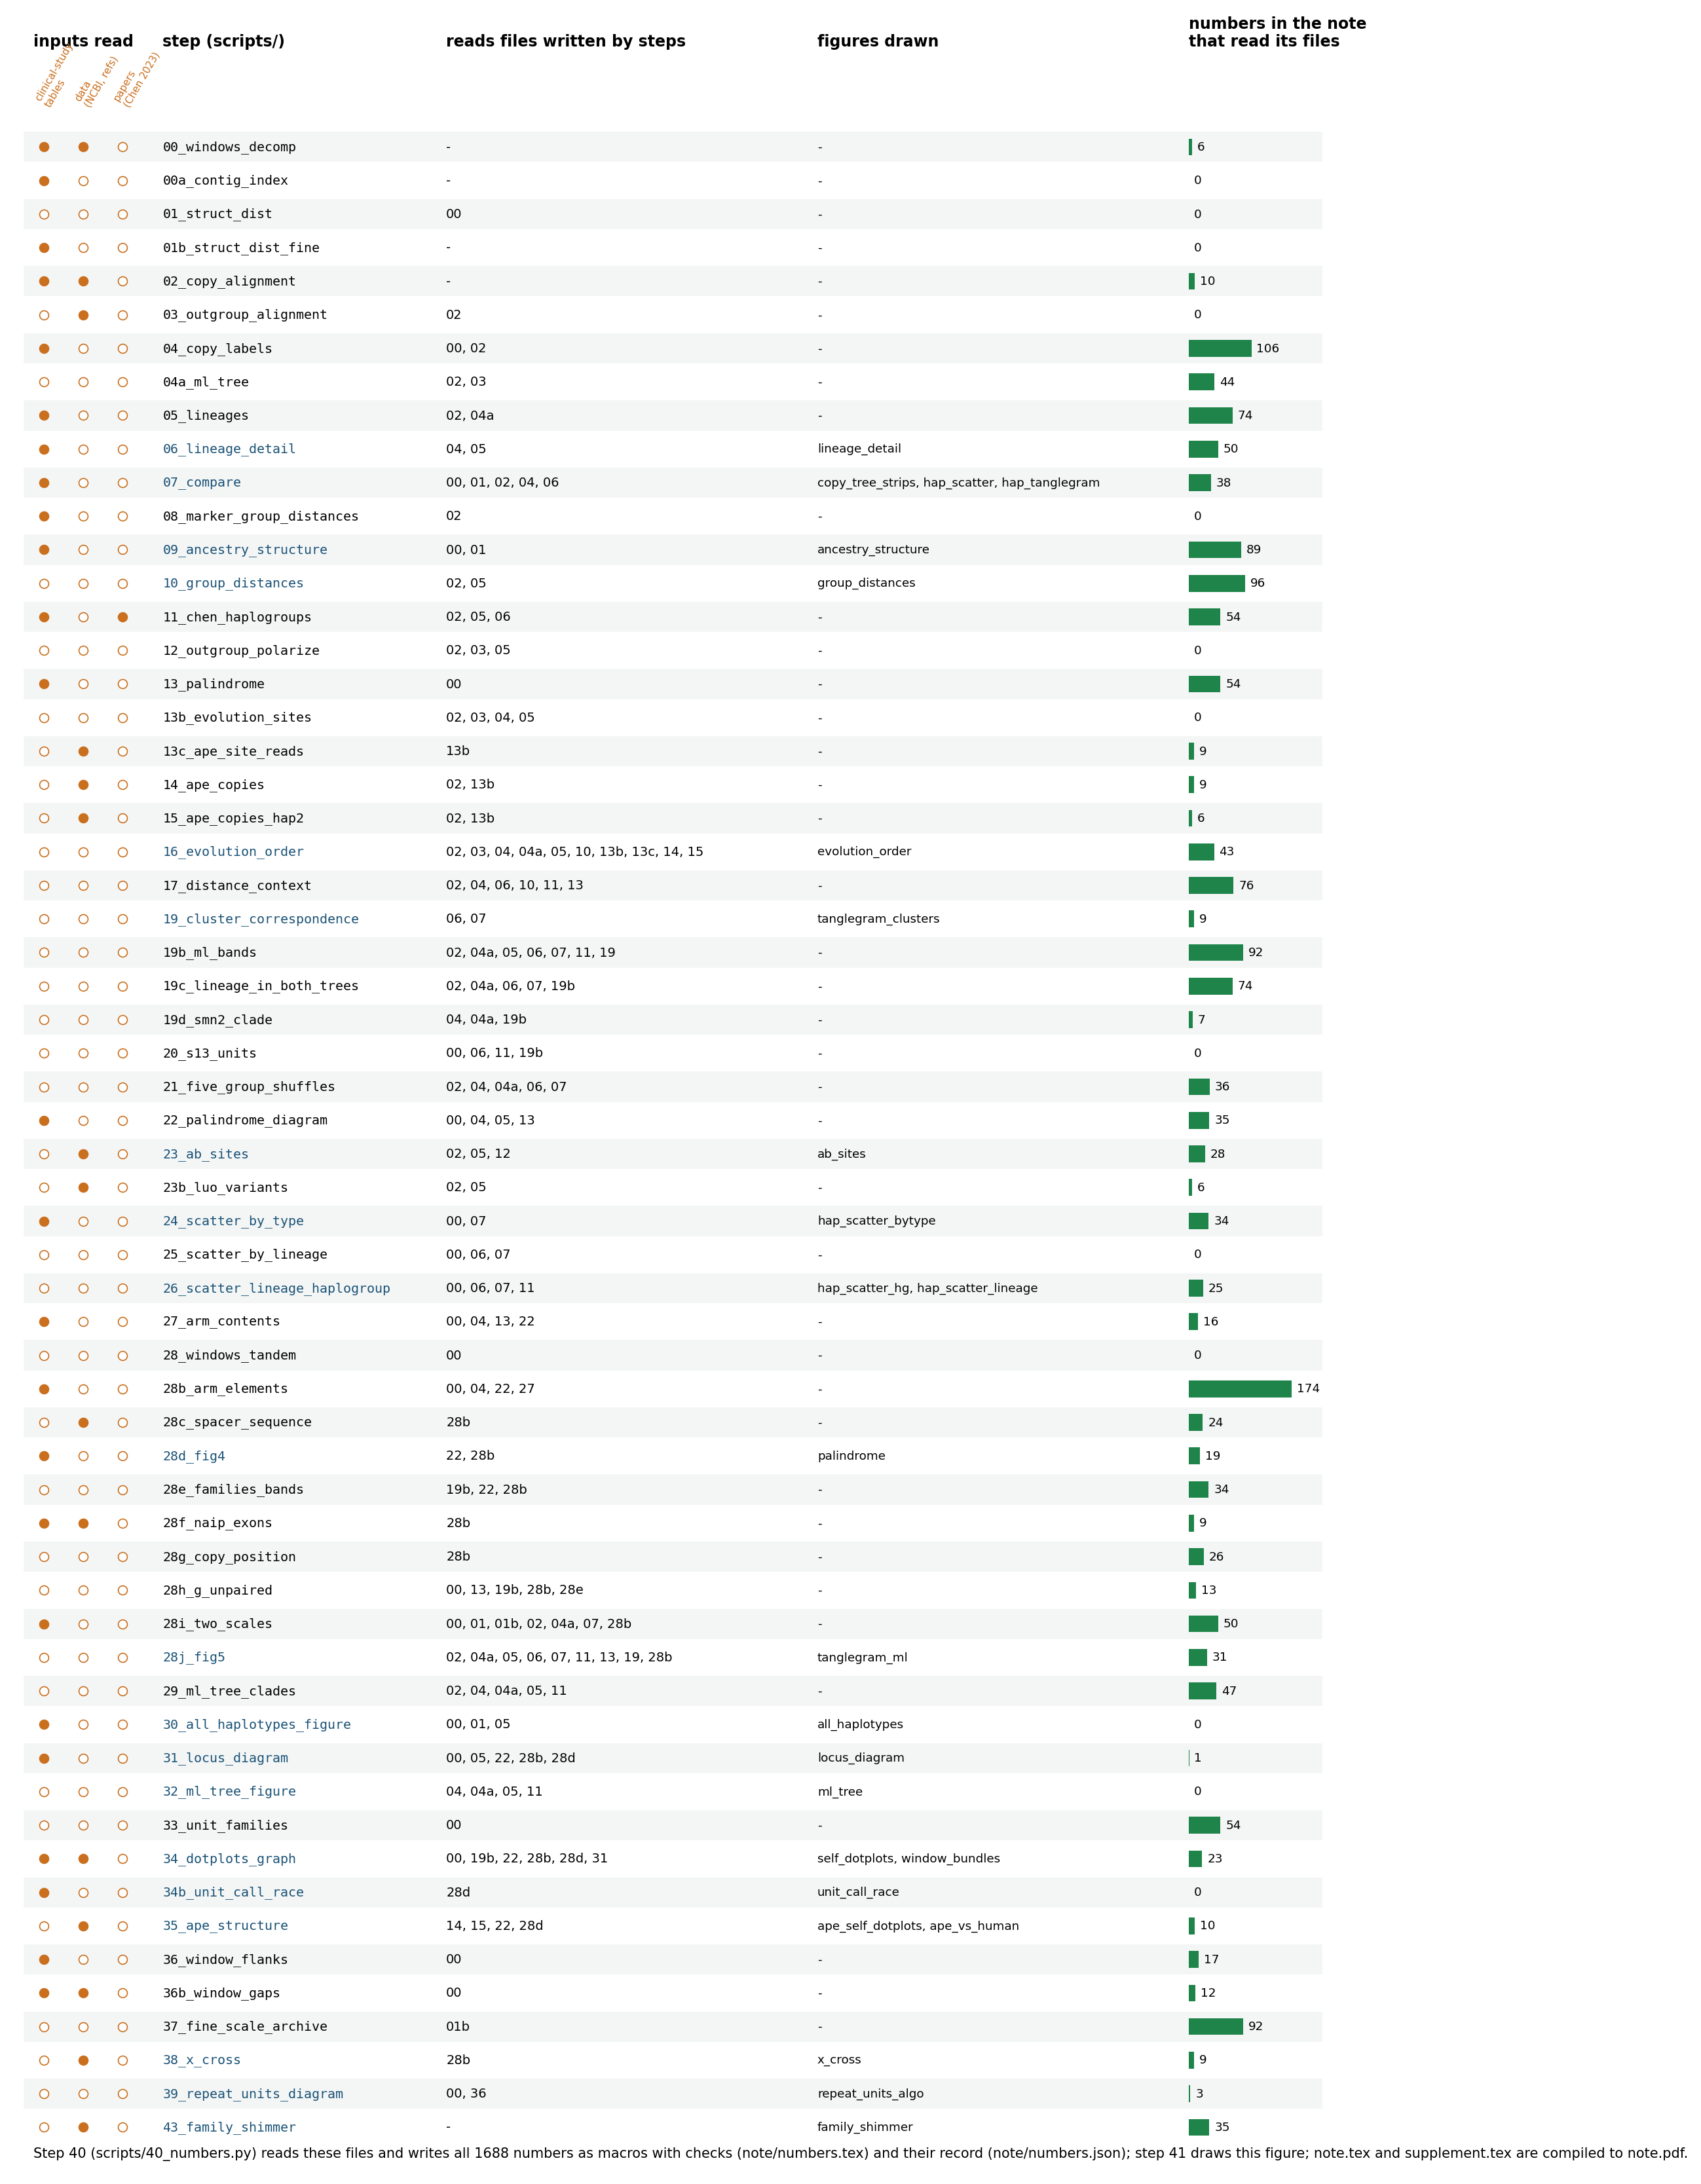
\includegraphics[width=\linewidth]{../figures/provenance.png}
\caption{The pipeline, one row per step in run order. Left, the inputs each step reads (orange dots: the clinical
study's tables, NCBI data and references, Chen et al.'s supplementary tables); then the earlier steps whose files it
reads; the figures it draws (step names in blue); and how many of the document's numbers read its files (green bars).
Python steps' reads and writes are traced at run time; shell steps' are declared. Drawn by
\texttt{41\_provenance.py} from \texttt{results/sv/provenance\_io.tsv} and \texttt{note/numbers.json}.}
\label{fig:provenance}
\end{figure}

{\footnotesize
\begin{longtable}{@{}>{\raggedright}p{5.6cm}>{\raggedright}p{1.4cm}r>{\raggedright}p{4.2cm}>{\raggedright\arraybackslash}p{2.2cm}@{}}
\caption{Where the numbers come from: each file the document's numbers read (in \texttt{results/sv/} unless a path is given), the step that writes it (``input'':
not written by this pipeline; ``setting'': a method setting read from a script), how many numbers read it, two of
them by macro name, and where the file is used (from \texttt{results/ledger.tsv}). Written by
\texttt{41\_provenance.py} from \texttt{note/numbers.json}.}\label{tab:numsrc}\\
\toprule
File & Step & Numbers & Example macros & Used in\\\midrule\endfirsthead
\toprule
File & Step & Numbers & Example macros & Used in\\\midrule\endhead
\tabNumSrc
\bottomrule
\end{longtable}}

\end{document}
